%
% part1.tex
%
% (c) 2018 Prof Dr Andreas Müller, Hochschule Rapperswil
%
\begin{refsection}
%
% vorwort.tex -- Vorwort zum Buch zum Seminar
%
% (c) 2019 Prof Dr Andreas Mueller, Hochschule Rapperswil
%
\chapter*{Vorwort}
\lhead{Vorwort}
\rhead{}
Dieses Buch entstand im Rahmen des Mathematischen Seminars
im Frühjahrssemester 2022 an der Ostschweizer Fachhochschule in Rapperswil.
Die Teilnehmer, Studierende der Studiengänge für Elektrotechnik,
Informatik und Bauingenieurwesen 
der OST, erarbeiteten nach einer Einführung in das Themengebiet jeweils
einzelne Aspekte des Gebietes in Form einer Seminararbeit, über
deren Resultate sie auch in einem Vortrag informierten. 

Im Frühjahr 2022 waren spezielle Funktionen das Thema des Seminars.
Ziel war, zu zeigen, wie neben den wohlbekannten Funktionen, die
man im elementaren Analysis-Unterricht kennenlernt, über die Jahre
viele weitere interessante Funktionen und Funktionenfamilien 
geschaffen wurden, mit denen die unterschiedlichsten Problem
auf effiziente Art gelöst werden können.

In einigen Arbeiten wurde auch Code zur Demonstration der 
besprochenen Methoden und Resultate geschrieben, soweit
möglich und sinnvoll wurde dieser Code im Github-Repository
\index{Github-Repository}%
dieses Kurses%
\footnote{\url{https://github.com/AndreasFMueller/SeminarSpezielleFunktionen.git}}
\cite{buch:repo}
abgelegt.
Im genannten Repository findet sich auch der Source-Code dieses
Skriptes, es wird hier unter einer Creative Commons Lizenz
zur Verfügung gestellt.


\part{Grundlagen}
%
% chapter.tex -- Beschreibung des Inhaltes
%
% (c) 2021 Prof Dr Andreas Müller, Hochschule Rapperswil
%
% !TeX spellcheck = de_CH
\chapter{Elliptische Funktionen
\label{buch:chapter:geometrie}}
\lhead{Elliptische Funktionen}
\rhead{}

Der Versuch, die Länge eines Ellipsenbogens zu berechnen, hat
in Abschnitt~\ref{buch:geometrie:subsection:hyperbeln-und-ellipsen}
zu Integralen geführt, die nicht in geschlossener Form ausgewertet
werden können.
Neben den dort gefundenen Integralen sind noch weitere, ähnlich
aufgebaute Integrale in dieser Familie zu finden.

%
% ellintegral.tex
%
% (c) 2021 Prof Dr Andreas Müller, OST Ostschweizer Fachhochschule
%
\section{Elliptische Integrale
\label{buch:elliptisch:section:integral}}
\rhead{Elliptisches Integral}
Bei der Berechnung des Ellipsenbogens in 
Abschnitt~\ref{buch:geometrie:subsection:hyperbeln-und-ellipsen}
sind wir auf ein Integral gestossen, welches sich nicht in geschlossener
Form ausdrücken liess.
Um solche Integrale in den Griff zu bekommen, ist es nötig, sie als
neue spezielle Funktionen zu definieren.

\subsection{Definition
\label{buch:elliptisch:subsection:definition}}
Ein {\em elliptisches Integral} ist ein Integral der Form
\index{elliptishes Integral}%
\index{Integral, elliptisch}%
\begin{equation}
\int R\left( x, \sqrt{p(x)}\right)\,dx
\label{buch:elliptisch:def:allgemein}
\end{equation}
wobei $R(x,y)$ eine rationale Funktion von zwei Variablen ist und
$p(x)$ ein Polynom dritten oder vierten Grades.
Hätte $p(x)$ ein mehrfache Nullstelle $x_0$, müsste es durch $(x-x_0)^2$
teilbar sein, man könnte also einen Faktor $(x-x_0)$ aus der
Wurzel im Integraneden von \eqref{buch:elliptisch:def:allgemein}
ausklammern und damit das Integral in eine Form bringen, wo $p(x)$
höchstens zweiten Grades ist.
Solche Integrale lassen sich meistens mit trigonometrischen Substitutionen
berechnen.
Wir verlangen daher, dass $p(x)$ keine mehrfachen Nullstellen hat.

Man kann zeigen, dass sich elliptische Integrale in Summen von
elementaren Funktionen und speziellen elliptischen Integralen 
der folgenden Form überführen lassen
\cite[Abschnitt 164, p.~506]{buch:smirnov32}.

\begin{definition}
\label{buch:elliptisch:def:integrale123}
Die elliptischen Integrale erster, zweiter und dritter Art sind die
Integrale
\[
\begin{aligned}
\text{1.~Art:}&&&
\int \frac{dx}{\sqrt{(1-x^2)(1-k^2x^2)}}
\\
\text{2.~Art:}&&&
\int \sqrt{\frac{1-k^2x^2}{1-x^2}}\,dx
\\
\text{3.~Art:}&&&
\int \frac{dx}{(1-nx^2)\sqrt{(1-x^2)(1-k^2x^2)}}
\end{aligned}
\]
mit $0<k<1$.
Es ist auch üblich, den Parameter $m=k^2$ zu verwenden.
\end{definition}

Wie gesagt lassen sich für diese unbestimmten Integrale keine 
geschlossenen Formen finden.
Es bleibt uns daher nichts anderes übrig, als die Integralgrenzen
festzulegen und damit eine Stammfunktion auszuwählen.

%
% Elliptisches Integral
%
\subsection{Vollständige elliptische Integrale
\label{buch:elliptisch:subsection:vollstaendig}}
In diesem Abschnitt legen wir beide Integrationsgrenzen fest und
untersuchen die entstehenenden Funktionen von den Parametern
$k$ und $n$.

\subsubsection{Definition der vollständigen elliptischen Integrale}
Da der Nenner in allen drei elliptischen Integralen eine Nullstelle
bei $\pm1$ hat, kann das Integral nur von $0$ bis $1$ erstreckt werden.

\begin{definition}
\label{buch:elliptisch:def:vollstintegrale123}
Die vollständigen elliptischen Integrale erster, zweiter und dritter
Art sind
\[
\begin{aligned}
\text{1.~Art:}&&
K(k)&=\int_0^1 \frac{dt}{\sqrt{(1-t^2)(1-k^2t^2)}} \\
\text{2.~Art:}&&
E(k)&=\int_0^1 \sqrt{\frac{1-k^2t^2}{1-t^2}}\,dt \\
\text{3.~Art:}&&
\Pi(n, k)&=\int_0^1\frac{dt}{(1-nt^2)\sqrt{(1-t^2)(1-k^2t^2)}} 
\end{aligned}
\]
mit $0<k<1$.
\end{definition}

Die Funktionen hängen stetig von $k$ ab.
Die Nullstellen des Faktors $1-k^2x^2$ liegen ausserhalb des
Integrationsintervalls und spielen daher keine Rolle.
Die Werte von $K(k)$ und $E(k)$ für $k=0$ können direkt berechnet
werden:
\begin{align*}
K(0)
=
E(0)
&=
\int_0^1 \frac{dt}{\sqrt{1-t^2}}=\frac{\pi}2.
\end{align*}
Das Integral $\Pi(n,0)$ ist etwas komplizierter.

Für $k\to 1$ ist $E(k)=1$, die Integrale $K(1)$ und $\Pi(n,1)$
sind dagegen divergent.

\subsubsection{Jacobi- und Legendre-Normalform}
Die Integrationsvariable $t$ der vollständigen elliptischen Integrale
kann durch die Substitution $t=\sin\varphi$ durch die Variable
$\varphi$ und das Integral über das Intervall $[0,1]$ durch ein
Integral über das Intervall $[0,\frac{\pi}2]$ ersetzt werden.
Mit
\[
\frac{dt}{d\varphi} = \cos\varphi = \sqrt{1-\sin^2\varphi}
\]
können die Funktionen $K(k)$, $E(k)$ und $\Pi(n,k)$ auch als
\begin{align*}
K(k)
&=
\int_0^{\frac{\pi}2}
\frac{
\sqrt{1-\sin^2\varphi}\,d\varphi
}{
\sqrt{(1-\sin^2\varphi)(1-k^2\sin^2\varphi)}
}
=
\int_0^{\frac{\pi}2}
\frac{d\varphi}{\sqrt{1-k^2\sin^2\varphi}}
\\
E(k)
&=
\int_0^{\frac{\pi}2}
\sqrt{\frac{1-k^2\sin^2\varphi}{1-\sin^2\varphi}}\sqrt{1-\sin^2\varphi}\,d\varphi
=
\int_0^{\frac{\pi}2}
\sqrt{1-k^2\sin^2\varphi}\,d\varphi
\\
\Pi(n,k)
&=
\int_0^{\frac{\pi}2}
\frac{
\sqrt{1-\sin^2\varphi}\,d\varphi
}{
(1-n\sin^2\varphi)\sqrt{(1-\sin^2\varphi)(1-k^2\sin^2\varphi)}
}
=
\int_0^{\frac{\pi}2}
\frac{
d\varphi
}{
(1-n\sin^2\varphi)\sqrt{1-k^2\sin^2\varphi}
}
\end{align*}
Diese Form wird auch die {\em Legendre-Normalform} der vollständigen 
\index{Legendre-Normalform}%
elliptischen Integrale genannt, während die Form von
Definition~\ref{buch:elliptisch:def:vollstintegrale123}
die {\em Jacobi-Normalform} heisst.
\index{Jacobi-Normalform}%

\subsubsection{Umfang einer Ellipse}
\begin{figure}
\centering
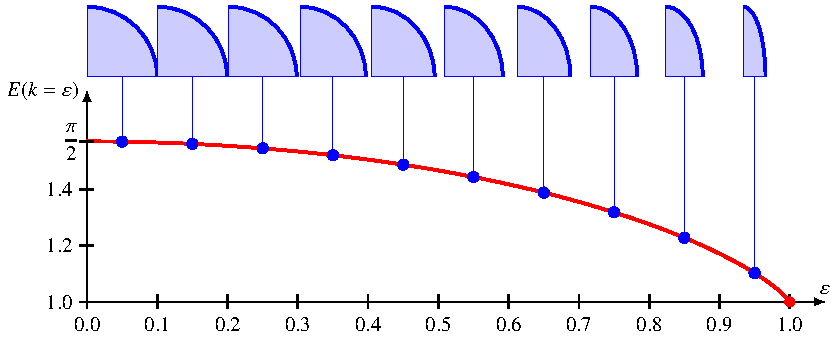
\includegraphics{chapters/110-elliptisch/images/ellipsenumfang.pdf}
\caption{Bogenlänge eines Viertels einer Ellipse mit Exzentrizität
$\varepsilon$.
\label{buch:elliptisch:fig:ellipsenumfang}}
\end{figure}
Wir zeigen, wie sich die Berechnung des Umfangs $U$ einer Ellipse
mit Halbachsen $a$ und $b$, $a\le b$, auf ein volltändiges elliptisches
Integral zurückführen lässt.
Der Fall $a>b$ kann behandelt werden, indem die $x$- und $y$-Koordinaten
vertauscht werden.

Die Parametrisierung
\[
t\mapsto \begin{pmatrix}a\cos t\\ b\sin t\end{pmatrix}
\]
einer Ellipse führt auf das Integral
\begin{align*}
U
&=
\int_0^{2\pi} \sqrt{a^2\sin^2t + b^2\cos^2 t}\,dt
\notag
\\
&=
4\int_0^{\frac{\pi}2}
\sqrt{a^2\sin^2t + b^2(1-\sin^2 t)}
\,dt
\notag
\\
&=
4b \int_0^{\frac{\pi}2} \sqrt{1-(b^2-a^2)/b^2\cdot \sin^2t}\,dt
\label{buch:elliptisch:eqn:umfangellipse}
\end{align*}
für den Umfang der Ellipse.
Bei einem Kreis ist $a=b$ und der zweite Term unter der Wurzel fällt weg,
der Umfang wird $4b\frac{\pi}2=2\pi b$.
Die Differenz $e^2=b^2-a^2$ ist die {\em lineare Exzentrizität} der Ellipse,
\index{lineare Exzentrizität}%
der Quotient $e/b$ wird die {\em numerische Exzentrizität} der Ellipse
genannt.
Insbesondere ist $k = \varepsilon$.

Das Integral~\eqref{buch:elliptisch:eqn:umfangellipse} erhält jetzt die
Form
\[
U
=
4b\int_0^{\frac{\pi}2} \sqrt{1-k^2\sin^2t}\,dt
\]
und ist damit als elliptisches Integral zweiter Art erkannt.
Für den Umfang der Ellipse finden wir damit die Formel
\[
U
=
4b E(k)
=
4b E(\varepsilon).
\]
Das vollständige elliptische Integral zweiter Art $E(\varepsilon)$
liefert also genau den Umfang der eines Viertels Ellipse mit
numerischer Exzentrizität $\varepsilon$ und kleiner Halbachse $1$.

\subsubsection{Komplementäre Integrale}
XXX Komplementäre Integrale \\

\subsubsection{Ableitung}
XXX Ableitung \\
XXX Stammfunktion \\

\subsection{Unvollständige elliptische Integrale}
XXX Vollständige und Unvollständige Integrale \\
XXX Additionstheoreme \\
XXX Parameterkonventionen \\

\subsection{Potenzreihe}
XXX Potenzreihen \\
XXX Als hypergeometrische Funktionen \\



\section{Jacobische elliptische Funktionen}

Für das elliptische Filter werden, wie es der Name bereits deutet, elliptische Funktionen gebraucht.
Wie die trigonometrischen Funktionen Zusammenhänge eines Kreises darlegen, beschreiben die elliptischen Funktionen Ellipsen.
Es ist daher naheliegend, dass der Kosinus des Tschebyscheff-Filters gegen ein elliptisches Pendant ausgetauscht werden könnte.
Der Begriff elliptische Funktion wird für sehr viele Funktionen gebraucht, daher ist es hier wichtig zu erwähnen, dass es ausschliesslich um die Jacobischen elliptischen Funktionen geht.

\subsection{Grundlegende Eigenschaften}

Die Jacobi elliptischen Funktionen werden ausführlich im Kapitel \ref{buch:elliptisch:section:jacobi} behandelt.
Im Wesentlichen erweitern die Jacobi elliptischen Funktionen die trigonometrische Funktionen für Ellipsen.
Zum Beispiel gibt es analog zum Sinus den elliptischen $\sn(z, k)$.
Im Gegensatz zum den trigonometrischen Funktionen haben die elliptischen Funktionen zwei Parameter.
Den \textit{elliptische Modul} $k$, der die Exzentrizität der Ellipse parametrisiert und das Winkelargument $z$.
Im Kreis ist der Radius für alle Winkel konstant, bei Ellipsen ändert sich das.
Dies hat zur Folge, dass bei einer Ellipse die Kreisbogenlänge nicht linear zum Winkel verläuft.
Darum kann hier nicht der gewohnte Winkel verwendet werden.
Das Winkelargument $z$ kann durch das elliptische Integral erster Art
\begin{equation}
    z
    =
    F(\phi, k)
    =
    \int_{0}^{\phi}
    \frac{
        d\theta
    }{
        \sqrt{
            1-k^2 \sin^2 \theta
        }
    }
\end{equation}
mit dem Winkel $\phi$ in Verbindung gebracht werden.

Dabei wird das vollständige und unvollständige elliptische integral unterschieden.
Beim vollständigen Integral
\begin{equation}
    K(k)
    =
    \int_{0}^{\pi / 2}
    \frac{
        d\theta
    }{
        \sqrt{
            1-k^2 \sin^2 \theta
        }
    }
\end{equation}
wird über ein viertel Ellipsenbogen integriert, also bis $\phi=\pi/2$ und liefert das Winkelargument für eine Vierteldrehung.
Die Zahl wird oft auch abgekürzt mit $K = K(k)$ und ist für das elliptische Filter sehr relevant.
Alle elliptischen Funktionen sind somit $4K$-periodisch.

Neben dem $\sn$ gibt es zwei weitere elliptische Basisfunktionen $\cn$ und $\dn$.
Dazu kommen noch weitere abgeleitete Funktionen, die durch Quotienten und Kehrwerte dieser Funktionen zustande kommen.
Insgesamt sind es die zwölf Funktionen
\begin{equation*}
    \sn \quad
    \ns \quad
    \scelliptic \quad
    \sd \quad
    \cn \quad
    \nc \quad
    \cs \quad
    \cd \quad
    \dn \quad
    \nd \quad
    \ds \quad
    \dc.
\end{equation*}

Die Jacobischen elliptischen Funktionen können mit der inversen Funktion des vollständigen elliptischen Integrals erster Art
\begin{equation}
    \phi = F^{-1}(z, k)
\end{equation}
definiert werden. Dabei ist zu beachten dass nur das $z$ Argument der Funktion invertiert wird, also
\begin{equation}
    z = F(\phi, k)
    \Leftrightarrow
    \phi = F^{-1}(z, k).
\end{equation}
Mithilfe von $F^{-1}$ kann zum Beispiel $sn^{-1}$ mit dem elliptischen Integral dargestellt werden:
\begin{equation}
    \sin(\phi)
    =
    \sin \left( F^{-1}(z, k) \right)
    =
    \sn(z, k)
    =
    w.
\end{equation}

% \begin{equation} %TODO remove unnecessary equations
%     \phi
%     =
%      F^{-1}(z, k)
%      =
%      \sin^{-1} \big( \sn (z, k ) \big)
%      =
%     \sin^{-1} ( w )
% \end{equation}

% \begin{equation}
%     F(\phi, k)
%     =
%     z
%     =
%     F( \sin^{-1} \big( \sn (z, k ) \big) , k)
%     =
%     F( \sin^{-1} ( w ), k)
% \end{equation}

% \begin{equation}
%     \sn^{-1}(w, k)
%     =
%     F(\phi, k),
%     \quad
%     \phi = \sin^{-1}(w)
% \end{equation}

\subsection{Die Funktion $\sn^{-1}$}

Beim Tschebyscheff-Filter konnten wir mit Betrachten des Arcuscosinus die Funktionalität erklären.
Für das Elliptische Filter machen wir die gleiche Betrachtung mit der $\sn^{-1}$-Funktion.
Der $\sn^{-1}$ ist durch das elliptische Integral
\begin{align}
    \sn^{-1}(w, k)
        & =
    \int_{0}^{\phi}
    \frac{
        d\theta
    }{
        \sqrt{
            1-k^2 \sin^2 \theta
        }
    },
    \quad
    \phi = \sin^{-1}(w)
    \\
        & =
    \int_{0}^{w}
    \frac{
        dt
    }{
        \sqrt{
            (1-t^2)(1-k^2 t^2)
        }
    }
\end{align}
beschrieben.
Dazu betrachten wir wieder den Integranden
\begin{equation}
    \frac{
        1
    }{
        \sqrt{
            (1-t^2)(1-k^2 t^2)
        }
    }.
\end{equation}
Beim $\cos^{-1}(x)$ haben wir gesehen, dass die analytische Fortsetzung bei $x < -1$ und $x > 1$ rechtwinklig in die komplexen Zahlen wandert.
Wenn man das Gleiche mit $\sn^{-1}(w, k)$ macht, erkennt man zwei interessante Stellen.
Die erste ist die gleiche wie beim $\cos^{-1}(x)$ nämlich bei $t = \pm 1$.
Der erste Term unter der Wurzel wird dann negativ, während der zweite noch positiv ist, da $k \leq 1$.
Ab diesem Punkt knickt die Funktion in die imaginäre Richtung ab.
Bei $t = 1/k$ ist auch der zweite Term negativ und die Funktion verläuft in die negative reelle Richtung.
Abbildung \ref{ellfilter:fig:sn} zeigt den Verlauf der Funktion in der komplexen Ebene.
\begin{figure}
    \centering
    \begin{tikzpicture}[>=stealth', auto, node distance=2cm, scale=1.2]

    \tikzstyle{zero} = [draw, circle, inner sep =0, minimum height=0.15cm]

    \tikzset{pole/.style={cross out, draw=black, minimum size=(0.15cm-\pgflinewidth), inner sep=0pt, outer sep=0pt}}

    \begin{scope}[xscale=0.9, yscale=1.8]

        \draw[gray, ->] (0,-1.5) -- (0,1.5) node[anchor=south]{$\mathrm{Im}~z$};
        \draw[gray, ->] (-5,0) -- (5,0) node[anchor=west]{$\mathrm{Re}~z$};

        \begin{scope}

            \clip(-4.5,-1.25) rectangle (4.5,1.25);

            \fill[yellow!30] (0,0) rectangle (1, 0.5);

            \begin{scope}[xshift=-1cm]

                \foreach \i in {-2,...,2} {
                    \foreach \j in {-2,...,1} {
                        \begin{scope}[xshift=\i*4cm, yshift=\j*1cm]
                            \draw[<-, blue!50] (0, 0) -- (0,0.5);
                            \draw[<-, cyan!50] (1, 0) -- (0,0);
                            \draw[<-, darkgreen!50] (2, 0) -- (1,0);
                            \draw[<-, orange!50] (2,0.5) -- (2, 0);
                            \draw[<-, red!50] (1, 0.5) -- (2,0.5);
                            \draw[<-, purple!50] (0, 0.5) -- (1,0.5);
                            \draw[<-, blue!50] (0,1) -- (0,0.5);
                            \draw[<-, orange!50] (2,0.5) -- (2, 1);
                            \draw[<-, red!50] (3, 0.5) -- (2,0.5);
                            \draw[<-, purple!50] (4, 0.5) -- (3,0.5);
                            \draw[<-, darkgreen!50] (2, 0) -- (3,0);
                            \draw[<-, cyan!50] (3, 0) -- (4,0);
                        \end{scope}
                    }
                }

                % \pause
                \draw[ultra thick, <-, darkgreen] (2, 0) -- (1,0);
                % \pause
                \draw[ultra thick, <-, orange] (2,0.5) -- (2, 0);
                % \pause
                \draw[ultra thick, <-, red] (1, 0.5) -- (2,0.5);
                % \pause
                \draw[ultra thick, <-, blue] (0, 0) -- (0,0.5);
                \draw[ultra thick, <-, purple] (0, 0.5) -- (1,0.5);
                \draw[ultra thick, <-, cyan] (1, 0) -- (0,0);
                % \pause


                \foreach \i in {-2,...,2} {
                    \foreach \j in {-2,...,1} {
                        \begin{scope}[xshift=\i*4cm, yshift=\j*1cm]
                            \node[zero] at ( 1, 0) {};
                            \node[zero] at ( 3, 0) {};
                            \node[pole] at ( 1,0.5) {};
                            \node[pole] at ( 3,0.5) {};
                        \end{scope}
                    }
                }

            \end{scope}

        \end{scope}

        \draw[gray] ( 1,0) +(0,0.1) -- +(0, -0.1) node[inner sep=0, anchor=north] {\small $K$};
        \draw[gray]  (0, 0.5) +(0.1, 0) -- +(-0.1, 0) node[inner sep=0, anchor=east]{\small $jK^\prime$};

    \end{scope}

    \node[zero] at (4,3) (n) {};
    \node[anchor=west] at (n.east) {Zero};
    \node[pole, below=0.25cm of n] (n) {};
    \node[anchor=west] at (n.east) {Pole};

    \begin{scope}[yshift=-4cm, xscale=0.75]

        \draw[gray, ->] (-6,0) -- (6,0) node[anchor=west]{$w$};

        \draw[ultra thick, ->, purple] (-5, 0) -- (-3, 0);
        \draw[ultra thick, ->, blue]      (-3, 0) -- (-2, 0);
        \draw[ultra thick, ->, cyan]       (-2, 0) -- (0, 0);
        \draw[ultra thick, ->, darkgreen]    (0, 0) -- (2, 0);
        \draw[ultra thick, ->, orange] (2, 0) -- (3, 0);
        \draw[ultra thick, ->, red] (3, 0) -- (5, 0);

        \node[anchor=south] at (-5,0) {$-\infty$};
        \node[anchor=south] at (-3,0) {$-1/k$};
        \node[anchor=south] at (-2,0) {$-1$};
        \node[anchor=south] at (0,0) {$0$};
        \node[anchor=south] at (2,0) {$1$};
        \node[anchor=south] at (3,0) {$1/k$};
        \node[anchor=south] at (5,0) {$\infty$};

    \end{scope}


\end{tikzpicture}
    \caption{
        $z$-Ebene der Funktion $z = \sn^{-1}(w, k)$.
        Die Funktion ist in der realen Achse $4K$-periodisch und in der imaginären Achse $2jK^\prime$-periodisch.
    }
    \label{ellfilter:fig:sn}
\end{figure}
In der reellen Richtung ist sie $4K(k)$-periodisch und in der imaginären Richtung $4K^\prime(k)$-periodisch, wobei $K^\prime$ das komplementäre vollständige Elliptische Integral ist:
\begin{equation}
    K^\prime(k)
    =
    \int_{0}^{\pi / 2}
    \frac{
        d\theta
    }{
        \sqrt{
            1-{k^\prime}^2 \sin^2 \theta
        }
    },
    \quad
    k^\prime = \sqrt{1-k^2}.
\end{equation}

%
% lemniskate.tex
%
% (c) 2021 Prof Dr Andreas Müller, OST Ostschweizer Fachhochschule
%
\section{Lemniskatischer Sinus
\label{buch:elliptisch:section:lemniskate}}
\rhead{Lemniskatischer Sinus}
Historisch war der {\em lemniskatische Sinus} die erste ellptische
Funktion, die Gauss bereits als 19-jähriger untersucht, aber nicht 
veröffentlich hat.
In diesem Abschnitt soll die Verbindung zu den Jacobischen
elliptischen Funktionen hergestellt werden.

\subsection{Lemniskate
\label{buch:gemotrie:subsection:lemniskate}}
\begin{figure}
\centering
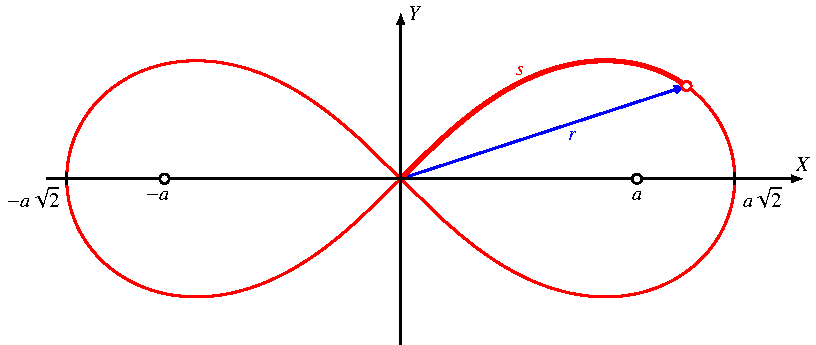
\includegraphics{chapters/110-elliptisch/images/lemniskate.pdf}
\caption{Bogenlänge und Radius der Lemniskate von Bernoulli.
\label{buch:elliptisch:fig:lemniskate}}
\end{figure}
Die Lemniskate von Bernoulli ist die Kurve vierten Grades mit der Gleichung
\begin{equation}
(X^2+Y^2)^2 = 2a^2(X^2-Y^2).
\label{buch:elliptisch:eqn:lemniskate}
\end{equation}
Sie ist in Abbildung~\ref{buch:elliptisch:fig:lemniskate}
dargestellt.
Die beiden Scheitel der Lemniskate befinden sich bei $X_s=\pm a\sqrt{2}$.
Dividiert man die Gleichung der Lemniskate durch $X_s^2=4a^4$ entsteht 
\begin{equation}
\biggl(
\biggl(\frac{X}{a\sqrt{2}}\biggr)^2
+
\biggl(\frac{Y}{a\sqrt{2}}\biggr)^2
\biggr)^2
=
2\frac{a^2}{2a^2}\biggl(
\biggl(\frac{X}{a\sqrt{2}}\biggr)^2
-
\biggl(\frac{Y}{a\sqrt{2}}\biggr)^2
\biggr).
\qquad
\Leftrightarrow
\qquad
(x^2+y^2)^2 = x^2-y^2,
\label{buch:elliptisch:eqn:lemniskatenormiert}
\end{equation}
wobei wir $x=X/a\sqrt{2}$ und $y=Y/a\sqrt{2}$ gesetzt haben.
In dieser Normierung liegen die Scheitel bei $\pm 1$.
Dies ist die Skalierung, die für die Definition des lemniskatischen
Sinus und Kosinus verwendet werden soll.

In Polarkoordinaten $x=r\cos\varphi$ und $y=r\sin\varphi$
gilt nach Einsetzen in \eqref{buch:elliptisch:eqn:lemniskatenormiert}
\begin{equation}
r^4
=
r^2(\cos^2\varphi-\sin^2\varphi)
=
r^2\cos2\varphi
\qquad\Rightarrow\qquad
r^2 = \cos 2\varphi
\label{buch:elliptisch:eqn:lemniskatepolar}
\end{equation}
als Darstellung der Lemniskate in Polardarstellung.
Sie gilt für Winkel $\varphi\in[-\frac{\pi}4,\frac{\pi}4]$ für das
rechte Blatt und $\varphi\in[\frac{3\pi}4,\frac{5\pi}4]$ für das linke
Blatt der Lemniskate.

\subsection{Bogenlänge}
Die Funktionen
\begin{equation}
x(r) = \frac{r}{\sqrt{2}}\sqrt{1+r^2},
\quad
y(r) = \frac{r}{\sqrt{2}}\sqrt{1-r^2}
\label{buch:geometrie:eqn:lemniskateparam}
\end{equation}
erfüllen
\begin{align*}
x(r)^2-y(r)^2
&=
\frac{r^2(1+r^2)}{2}-\frac{r^2(1-r^2)}{2}
\\
&
=
r^4
=
(x(r)^2 + y(r)^2)^2,
\end{align*}
sie stellen also eine Parametrisierung der Lemniskate dar.

Mit Hilfe der Parametrisierung~\eqref{buch:geometrie:eqn:lemniskateparam}
kann man die Länge $s$ des in Abbildung~\ref{buch:elliptisch:fig:lemniskate}
dargestellten Bogens der Lemniskate berechnen.
Dazu benötigt man die Ableitungen nach $r$, die man mit der Produkt- und
Kettenregel berechnen kann:
\begin{align*}
\dot{x}(r)
&=
\frac{\sqrt{1+r^2}}{\sqrt{2}}
+
\frac{r^2}{\sqrt{2}\sqrt{1+r^2}}
&&\Rightarrow&
\dot{x}(r)^2
&=
\frac{1+r^2}{2} +r^2 + \frac{r^4}{2(1+r^2)}
\\
\dot{y}(r)
&=
\frac{\sqrt{1-r^2}}{\sqrt{2}}
-
\frac{r^2}{\sqrt{2}\sqrt{1-r^2}}
&&\Rightarrow&
\dot{y}(r)^2
&=
\frac{1-r^2}{2} -r^2 + \frac{r^4}{2(1-r^2)}
\end{align*}
Die Summe der Quadrate ist
\begin{align*}
\dot{x}(r)^2 + \dot{y}(r)^2
&=
1 + r^4\frac{1-r^2+1+r^2}{2(1+r^2)(1-r^2)}
=
1+r^4\frac{2}{2(1-r^4)}
=
\frac{1-r^4+r^4}{1-r^4}
=
\frac1{1-r^4}.
\end{align*}
Durch Einsetzen in das Integral für die Bogenlänge bekommt man
\begin{equation}
s(r)
=
\int_0^r
\frac{1}{\sqrt{1-t^4}}\,dt.
\label{buch:elliptisch:eqn:lemniskatebogenlaenge}
\end{equation}

%
% Als elliptisches Integral
%
\subsection{Darstellung als elliptisches Integral}
Das unvollständige elliptische Integral erster Art mit Parameter
$k^2=-1$ oder $k=i$ ist
\[
K(r,i)
=
\int_0^x \frac{dt}{\sqrt{(1-t^2)(1-i^2 t^2)}}
=
\int_0^x \frac{dt}{\sqrt{(1-t^2)(1-(-1)t^2)}}
=
\int_0^x \frac{dt}{\sqrt{1-t^4}}
=
s(r).
\]
Der lemniskatische Sinus ist also eine Umkehrfunktion des
elliptischen Integrals erster Art für den speziellen Wert $i$ des
Parameters $k$.

Die Länge des rechten Blattes der Lemniskate wird mit $\varpi$ bezeichnet
und hat den numerischen Wert
\[
\varpi
=
2\int_0^1\sqrt{\frac{1}{1-t^4}}\,dt
=
2.6220575542.
\]
$\varpi$ ist auch als die {\em lemniskatische Konstante} bekannt.
\index{lemniskatische Konstante}%
Der Lemniskatenbogen zwischen dem Nullpunkt und $(1,0)$ hat die Länge
$\varpi/2$.

%
%  Bogenlängenparametrisierung
%
\subsection{Bogenlängenparametrisierung}
Die Lemniskate mit der Gleichung
\[
(X^2+X^2)^2=2(X^2-X^2)
\]
(der Fall $a=1$ in \eqref{buch:elliptisch:eqn:lemniskate})
kann mit Jacobischen elliptischen Funktionen
parametrisiert werden.
Dazu schreibt man
\[
\left.
\begin{aligned}
X(t)
&=
\sqrt{2}\operatorname{cn}(t,k) \operatorname{dn}(t,k)
\\
Y(t)
&=
\phantom{\sqrt{2}}
\operatorname{cn}(t,k) \operatorname{sn}(t,k)
\end{aligned}
\quad\right\}
\qquad\text{mit $k=\displaystyle\frac{1}{\sqrt{2}}$}
\]
und berechnet die beiden Seiten der definierenden Gleichung der
Lemniskate.
Zunächst ist
\begin{align*}
X(t)^2
&=
2\operatorname{cn}(t,k)^2
\operatorname{dn}(t,k)^2
\\
Y(t)^2
&=
\operatorname{cn}(t,k)^2
\operatorname{sn}(t,k)^2
\\
X(t)^2+Y(t)^2
&=
2\operatorname{cn}(t,k)^2
\bigl(
\underbrace{
\operatorname{dn}(t,k)^2
+{\textstyle\frac12}
\operatorname{sn}(t,k)^2
}_{\displaystyle =1}
\bigr)
%\\
%&
=
2\operatorname{cn}(t,k)^2
\\
X(t)^2-Y(t)^2
&=
\operatorname{cn}(t,k)^2
\bigl(
2\operatorname{dn}(t,k)^2 - \operatorname{sn}(t,k)^2
\bigr)
\\
&=
\operatorname{cn}(t,k)^2
\bigl(
2\bigl({\textstyle\frac12}+{\textstyle\frac12}\operatorname{cn}(t,k)^2\bigr)
-
\bigl(1-\operatorname{cn}(t,k)^2\bigr)
\bigr)
\\
&=
2\operatorname{cn}(t,k)^4
\\
\Rightarrow\qquad
(X(t)^2+Y(t)^2)^2
&=
4\operatorname{cn}(t,k)^4
=
2(X(t)^2-Y(t)^2).
\end{align*}
Wir zeigen jetzt, dass dies tatsächlich eine Bogenlängenparametrisierung
der Lemniskate ist.
Dazu berechnen wir die Ableitungen
\begin{align*}
\dot{X}(t)
&=
\sqrt{2}\operatorname{cn}'(t,k)\operatorname{dn}(t,k)
+
\sqrt{2}\operatorname{cn}(t,k)\operatorname{dn}'(t,k)
\\
&=
-\sqrt{2}\operatorname{sn}(t,k)\operatorname{dn}(t,k)^2
-\frac12\sqrt{2}\operatorname{sn}(t,k)\operatorname{cn}(t,k)^2
\\
&=
-\sqrt{2}\operatorname{sn}(t,k)\bigl(
1-{\textstyle\frac12}\operatorname{sn}(t,k)^2
+{\textstyle\frac12}-{\textstyle\frac12}\operatorname{sn}(u,t)^2
\bigr)
\\
&=
\sqrt{2}\operatorname{sn}(t,k)
\bigl(
{\textstyle \frac32}-\operatorname{sn}(t,k)^2
\bigr)
\\
\dot{X}(t)^2
&=
2\operatorname{sn}(t,k)^2
\bigl(
{\textstyle \frac32}-\operatorname{sn}(t,k)^2
\bigr)^2
\\
&=
{\textstyle\frac{9}{2}}\operatorname{sn}(t,k)^2
-
6\operatorname{sn}(t,k)^4
+2\operatorname{sn}(t,k)^6
\\
\dot{Y}(t)
&=
\operatorname{cn}'(t,k)\operatorname{sn}(t,k)
+
\operatorname{cn}(t,k)\operatorname{sn}'(t,k)
\\
&=
-\operatorname{sn}(t,k)^2
\operatorname{dn}(t,k)
+\operatorname{cn}(t,k)^2
\operatorname{dn}(t,k)
\\
&=
\operatorname{dn}(t,k)\bigl(1-2\operatorname{sn}(t,k)^2\bigr)
\\
\dot{Y}(t)^2
&=
\bigl(1-{\textstyle\frac12}\operatorname{sn}(t,k)^2\bigr)
\bigl(1-2\operatorname|{sn}(t,k)^2\bigr)^2
\\
&=
1-{\textstyle\frac{9}{2}}\operatorname{sn}(t,k)^2
+6\operatorname{sn}(t,k)^4
-2\operatorname{sn}(t,k)^6
\\
\dot{X}(t)^2 + \dot{Y}(t)^2
&=
1.
\end{align*}
Dies bedeutet, dass die Bogenlänge zwischen den Parameterwerten $0$ und $s$
\[
\int_0^s
\sqrt{\dot{X}(t)^2 + \dot{Y}(t)^2}
\,dt
=
\int_0^s\,dt
=
s,
\]
der Parameter $t$ ist also ein Bogenlängenparameter.

Die mit dem Faktor $1/\sqrt{2}$ skalierte Standard-Lemniskate mit der
Gleichung
\[
(x^2+y^2)^2 = x^2-y^2
\]
hat daher eine Bogenlängenparametrisierung mit
\begin{equation}
\begin{aligned}
x(t)
&=
\phantom{\frac{1}{\sqrt{2}}}
\operatorname{cn}(\sqrt{2}t,k)\operatorname{dn}(\sqrt{2}t,k)
\\
y(t)
&=
\frac{1}{\sqrt{2}}\operatorname{cn}(\sqrt{2}t,k)\operatorname{sn}(\sqrt{2}t,k)
\end{aligned}
\label{buch:elliptisch:lemniskate:bogenlaenge}
\end{equation}

\subsection{Der lemniskatische Sinus und Kosinus}
Der Sinus Berechnet die Gegenkathete zu einer gegebenen Bogenlänge des
Kreises, er ist die Umkehrfunktion der Funktion, die der Gegenkathete
die Bogenlänge zuordnet.

Daher ist es naheliegend, die Umkehrfunktion von $s(r)$ in 
\eqref{buch:elliptisch:eqn:lemniskatebogenlaenge}
den {\em lemniskatischen Sinus} zu nennen mit der Bezeichnung
$r=\operatorname{sl} s$.

Der Kosinus ist der Sinus des komplementären Winkels.
Auch für die lemniskatische Bogenlänge $s(r)$ lässt sich eine
komplementäre Bogenlänge definieren, nämlich die Bogenlänge zwischen
dem Punkt $(x(r), y(r))$ und $(1,0)$.

Da die Parametrisierung~\eqref{buch:elliptisch:lemniskate:bogenlaenge}
eine Bogenlängenparametrisierung ist, darf man $t=s$ schreiben.
Dann kann man aber auch $r(s)$ daraus berechnen,
es ist
\[
r(s)^2
=
x(s)^2 + y(s)^2
=
\operatorname{cn}(s\sqrt{2},k)^2
\qquad\Rightarrow\qquad
r(s)
=
\operatorname{cn}(s\sqrt{2},k)
\]

\begin{figure}
\centering
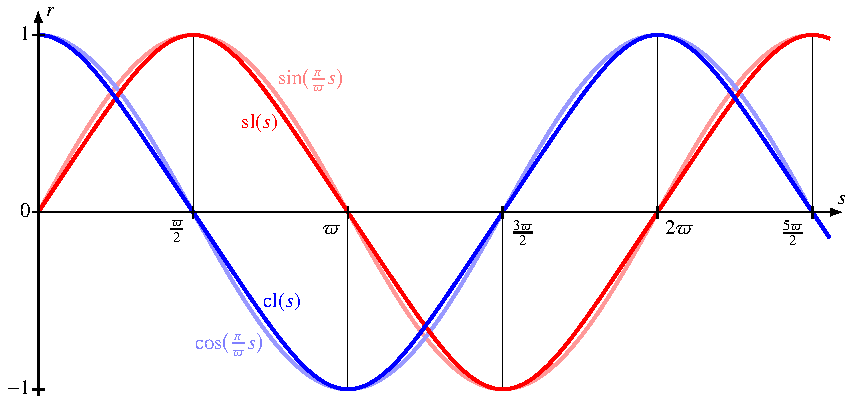
\includegraphics{chapters/110-elliptisch/images/slcl.pdf}
\caption{
Lemniskatischer Sinus und Kosinus sowie Sinus und Kosinus
mit derart skaliertem Argument, dass die Funktionen die gleichen Nullstellen
haben.
\label{buch:elliptisch:figure:slcl}}
\end{figure}


%\section*{Übungsaufgaben}
%\rhead{Übungsaufgaben}
%\aufgabetoplevel{chapters/020-exponential/uebungsaufgaben}
%\begin{uebungsaufgaben}
%\uebungsaufgabe{0}
%\uebungsaufgabe{1}
%\end{uebungsaufgaben}



% algebraisch und geometrisch definierte spezielle Funktionen
%
% chapter.tex -- Beschreibung des Inhaltes
%
% (c) 2021 Prof Dr Andreas Müller, Hochschule Rapperswil
%
% !TeX spellcheck = de_CH
\chapter{Elliptische Funktionen
\label{buch:chapter:geometrie}}
\lhead{Elliptische Funktionen}
\rhead{}

Der Versuch, die Länge eines Ellipsenbogens zu berechnen, hat
in Abschnitt~\ref{buch:geometrie:subsection:hyperbeln-und-ellipsen}
zu Integralen geführt, die nicht in geschlossener Form ausgewertet
werden können.
Neben den dort gefundenen Integralen sind noch weitere, ähnlich
aufgebaute Integrale in dieser Familie zu finden.

%
% ellintegral.tex
%
% (c) 2021 Prof Dr Andreas Müller, OST Ostschweizer Fachhochschule
%
\section{Elliptische Integrale
\label{buch:elliptisch:section:integral}}
\rhead{Elliptisches Integral}
Bei der Berechnung des Ellipsenbogens in 
Abschnitt~\ref{buch:geometrie:subsection:hyperbeln-und-ellipsen}
sind wir auf ein Integral gestossen, welches sich nicht in geschlossener
Form ausdrücken liess.
Um solche Integrale in den Griff zu bekommen, ist es nötig, sie als
neue spezielle Funktionen zu definieren.

\subsection{Definition
\label{buch:elliptisch:subsection:definition}}
Ein {\em elliptisches Integral} ist ein Integral der Form
\index{elliptishes Integral}%
\index{Integral, elliptisch}%
\begin{equation}
\int R\left( x, \sqrt{p(x)}\right)\,dx
\label{buch:elliptisch:def:allgemein}
\end{equation}
wobei $R(x,y)$ eine rationale Funktion von zwei Variablen ist und
$p(x)$ ein Polynom dritten oder vierten Grades.
Hätte $p(x)$ ein mehrfache Nullstelle $x_0$, müsste es durch $(x-x_0)^2$
teilbar sein, man könnte also einen Faktor $(x-x_0)$ aus der
Wurzel im Integraneden von \eqref{buch:elliptisch:def:allgemein}
ausklammern und damit das Integral in eine Form bringen, wo $p(x)$
höchstens zweiten Grades ist.
Solche Integrale lassen sich meistens mit trigonometrischen Substitutionen
berechnen.
Wir verlangen daher, dass $p(x)$ keine mehrfachen Nullstellen hat.

Man kann zeigen, dass sich elliptische Integrale in Summen von
elementaren Funktionen und speziellen elliptischen Integralen 
der folgenden Form überführen lassen
\cite[Abschnitt 164, p.~506]{buch:smirnov32}.

\begin{definition}
\label{buch:elliptisch:def:integrale123}
Die elliptischen Integrale erster, zweiter und dritter Art sind die
Integrale
\[
\begin{aligned}
\text{1.~Art:}&&&
\int \frac{dx}{\sqrt{(1-x^2)(1-k^2x^2)}}
\\
\text{2.~Art:}&&&
\int \sqrt{\frac{1-k^2x^2}{1-x^2}}\,dx
\\
\text{3.~Art:}&&&
\int \frac{dx}{(1-nx^2)\sqrt{(1-x^2)(1-k^2x^2)}}
\end{aligned}
\]
mit $0<k<1$.
Es ist auch üblich, den Parameter $m=k^2$ zu verwenden.
\end{definition}

Wie gesagt lassen sich für diese unbestimmten Integrale keine 
geschlossenen Formen finden.
Es bleibt uns daher nichts anderes übrig, als die Integralgrenzen
festzulegen und damit eine Stammfunktion auszuwählen.

%
% Elliptisches Integral
%
\subsection{Vollständige elliptische Integrale
\label{buch:elliptisch:subsection:vollstaendig}}
In diesem Abschnitt legen wir beide Integrationsgrenzen fest und
untersuchen die entstehenenden Funktionen von den Parametern
$k$ und $n$.

\subsubsection{Definition der vollständigen elliptischen Integrale}
Da der Nenner in allen drei elliptischen Integralen eine Nullstelle
bei $\pm1$ hat, kann das Integral nur von $0$ bis $1$ erstreckt werden.

\begin{definition}
\label{buch:elliptisch:def:vollstintegrale123}
Die vollständigen elliptischen Integrale erster, zweiter und dritter
Art sind
\[
\begin{aligned}
\text{1.~Art:}&&
K(k)&=\int_0^1 \frac{dt}{\sqrt{(1-t^2)(1-k^2t^2)}} \\
\text{2.~Art:}&&
E(k)&=\int_0^1 \sqrt{\frac{1-k^2t^2}{1-t^2}}\,dt \\
\text{3.~Art:}&&
\Pi(n, k)&=\int_0^1\frac{dt}{(1-nt^2)\sqrt{(1-t^2)(1-k^2t^2)}} 
\end{aligned}
\]
mit $0<k<1$.
\end{definition}

Die Funktionen hängen stetig von $k$ ab.
Die Nullstellen des Faktors $1-k^2x^2$ liegen ausserhalb des
Integrationsintervalls und spielen daher keine Rolle.
Die Werte von $K(k)$ und $E(k)$ für $k=0$ können direkt berechnet
werden:
\begin{align*}
K(0)
=
E(0)
&=
\int_0^1 \frac{dt}{\sqrt{1-t^2}}=\frac{\pi}2.
\end{align*}
Das Integral $\Pi(n,0)$ ist etwas komplizierter.

Für $k\to 1$ ist $E(k)=1$, die Integrale $K(1)$ und $\Pi(n,1)$
sind dagegen divergent.

\subsubsection{Jacobi- und Legendre-Normalform}
Die Integrationsvariable $t$ der vollständigen elliptischen Integrale
kann durch die Substitution $t=\sin\varphi$ durch die Variable
$\varphi$ und das Integral über das Intervall $[0,1]$ durch ein
Integral über das Intervall $[0,\frac{\pi}2]$ ersetzt werden.
Mit
\[
\frac{dt}{d\varphi} = \cos\varphi = \sqrt{1-\sin^2\varphi}
\]
können die Funktionen $K(k)$, $E(k)$ und $\Pi(n,k)$ auch als
\begin{align*}
K(k)
&=
\int_0^{\frac{\pi}2}
\frac{
\sqrt{1-\sin^2\varphi}\,d\varphi
}{
\sqrt{(1-\sin^2\varphi)(1-k^2\sin^2\varphi)}
}
=
\int_0^{\frac{\pi}2}
\frac{d\varphi}{\sqrt{1-k^2\sin^2\varphi}}
\\
E(k)
&=
\int_0^{\frac{\pi}2}
\sqrt{\frac{1-k^2\sin^2\varphi}{1-\sin^2\varphi}}\sqrt{1-\sin^2\varphi}\,d\varphi
=
\int_0^{\frac{\pi}2}
\sqrt{1-k^2\sin^2\varphi}\,d\varphi
\\
\Pi(n,k)
&=
\int_0^{\frac{\pi}2}
\frac{
\sqrt{1-\sin^2\varphi}\,d\varphi
}{
(1-n\sin^2\varphi)\sqrt{(1-\sin^2\varphi)(1-k^2\sin^2\varphi)}
}
=
\int_0^{\frac{\pi}2}
\frac{
d\varphi
}{
(1-n\sin^2\varphi)\sqrt{1-k^2\sin^2\varphi}
}
\end{align*}
Diese Form wird auch die {\em Legendre-Normalform} der vollständigen 
\index{Legendre-Normalform}%
elliptischen Integrale genannt, während die Form von
Definition~\ref{buch:elliptisch:def:vollstintegrale123}
die {\em Jacobi-Normalform} heisst.
\index{Jacobi-Normalform}%

\subsubsection{Umfang einer Ellipse}
\begin{figure}
\centering
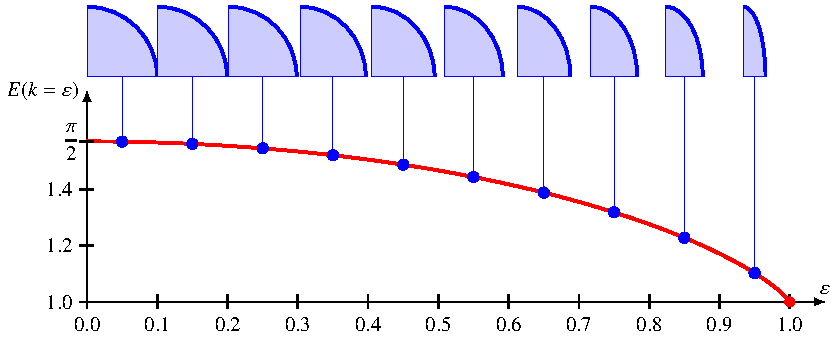
\includegraphics{chapters/110-elliptisch/images/ellipsenumfang.pdf}
\caption{Bogenlänge eines Viertels einer Ellipse mit Exzentrizität
$\varepsilon$.
\label{buch:elliptisch:fig:ellipsenumfang}}
\end{figure}
Wir zeigen, wie sich die Berechnung des Umfangs $U$ einer Ellipse
mit Halbachsen $a$ und $b$, $a\le b$, auf ein volltändiges elliptisches
Integral zurückführen lässt.
Der Fall $a>b$ kann behandelt werden, indem die $x$- und $y$-Koordinaten
vertauscht werden.

Die Parametrisierung
\[
t\mapsto \begin{pmatrix}a\cos t\\ b\sin t\end{pmatrix}
\]
einer Ellipse führt auf das Integral
\begin{align*}
U
&=
\int_0^{2\pi} \sqrt{a^2\sin^2t + b^2\cos^2 t}\,dt
\notag
\\
&=
4\int_0^{\frac{\pi}2}
\sqrt{a^2\sin^2t + b^2(1-\sin^2 t)}
\,dt
\notag
\\
&=
4b \int_0^{\frac{\pi}2} \sqrt{1-(b^2-a^2)/b^2\cdot \sin^2t}\,dt
\label{buch:elliptisch:eqn:umfangellipse}
\end{align*}
für den Umfang der Ellipse.
Bei einem Kreis ist $a=b$ und der zweite Term unter der Wurzel fällt weg,
der Umfang wird $4b\frac{\pi}2=2\pi b$.
Die Differenz $e^2=b^2-a^2$ ist die {\em lineare Exzentrizität} der Ellipse,
\index{lineare Exzentrizität}%
der Quotient $e/b$ wird die {\em numerische Exzentrizität} der Ellipse
genannt.
Insbesondere ist $k = \varepsilon$.

Das Integral~\eqref{buch:elliptisch:eqn:umfangellipse} erhält jetzt die
Form
\[
U
=
4b\int_0^{\frac{\pi}2} \sqrt{1-k^2\sin^2t}\,dt
\]
und ist damit als elliptisches Integral zweiter Art erkannt.
Für den Umfang der Ellipse finden wir damit die Formel
\[
U
=
4b E(k)
=
4b E(\varepsilon).
\]
Das vollständige elliptische Integral zweiter Art $E(\varepsilon)$
liefert also genau den Umfang der eines Viertels Ellipse mit
numerischer Exzentrizität $\varepsilon$ und kleiner Halbachse $1$.

\subsubsection{Komplementäre Integrale}
XXX Komplementäre Integrale \\

\subsubsection{Ableitung}
XXX Ableitung \\
XXX Stammfunktion \\

\subsection{Unvollständige elliptische Integrale}
XXX Vollständige und Unvollständige Integrale \\
XXX Additionstheoreme \\
XXX Parameterkonventionen \\

\subsection{Potenzreihe}
XXX Potenzreihen \\
XXX Als hypergeometrische Funktionen \\



\section{Jacobische elliptische Funktionen}

Für das elliptische Filter werden, wie es der Name bereits deutet, elliptische Funktionen gebraucht.
Wie die trigonometrischen Funktionen Zusammenhänge eines Kreises darlegen, beschreiben die elliptischen Funktionen Ellipsen.
Es ist daher naheliegend, dass der Kosinus des Tschebyscheff-Filters gegen ein elliptisches Pendant ausgetauscht werden könnte.
Der Begriff elliptische Funktion wird für sehr viele Funktionen gebraucht, daher ist es hier wichtig zu erwähnen, dass es ausschliesslich um die Jacobischen elliptischen Funktionen geht.

\subsection{Grundlegende Eigenschaften}

Die Jacobi elliptischen Funktionen werden ausführlich im Kapitel \ref{buch:elliptisch:section:jacobi} behandelt.
Im Wesentlichen erweitern die Jacobi elliptischen Funktionen die trigonometrische Funktionen für Ellipsen.
Zum Beispiel gibt es analog zum Sinus den elliptischen $\sn(z, k)$.
Im Gegensatz zum den trigonometrischen Funktionen haben die elliptischen Funktionen zwei Parameter.
Den \textit{elliptische Modul} $k$, der die Exzentrizität der Ellipse parametrisiert und das Winkelargument $z$.
Im Kreis ist der Radius für alle Winkel konstant, bei Ellipsen ändert sich das.
Dies hat zur Folge, dass bei einer Ellipse die Kreisbogenlänge nicht linear zum Winkel verläuft.
Darum kann hier nicht der gewohnte Winkel verwendet werden.
Das Winkelargument $z$ kann durch das elliptische Integral erster Art
\begin{equation}
    z
    =
    F(\phi, k)
    =
    \int_{0}^{\phi}
    \frac{
        d\theta
    }{
        \sqrt{
            1-k^2 \sin^2 \theta
        }
    }
\end{equation}
mit dem Winkel $\phi$ in Verbindung gebracht werden.

Dabei wird das vollständige und unvollständige elliptische integral unterschieden.
Beim vollständigen Integral
\begin{equation}
    K(k)
    =
    \int_{0}^{\pi / 2}
    \frac{
        d\theta
    }{
        \sqrt{
            1-k^2 \sin^2 \theta
        }
    }
\end{equation}
wird über ein viertel Ellipsenbogen integriert, also bis $\phi=\pi/2$ und liefert das Winkelargument für eine Vierteldrehung.
Die Zahl wird oft auch abgekürzt mit $K = K(k)$ und ist für das elliptische Filter sehr relevant.
Alle elliptischen Funktionen sind somit $4K$-periodisch.

Neben dem $\sn$ gibt es zwei weitere elliptische Basisfunktionen $\cn$ und $\dn$.
Dazu kommen noch weitere abgeleitete Funktionen, die durch Quotienten und Kehrwerte dieser Funktionen zustande kommen.
Insgesamt sind es die zwölf Funktionen
\begin{equation*}
    \sn \quad
    \ns \quad
    \scelliptic \quad
    \sd \quad
    \cn \quad
    \nc \quad
    \cs \quad
    \cd \quad
    \dn \quad
    \nd \quad
    \ds \quad
    \dc.
\end{equation*}

Die Jacobischen elliptischen Funktionen können mit der inversen Funktion des vollständigen elliptischen Integrals erster Art
\begin{equation}
    \phi = F^{-1}(z, k)
\end{equation}
definiert werden. Dabei ist zu beachten dass nur das $z$ Argument der Funktion invertiert wird, also
\begin{equation}
    z = F(\phi, k)
    \Leftrightarrow
    \phi = F^{-1}(z, k).
\end{equation}
Mithilfe von $F^{-1}$ kann zum Beispiel $sn^{-1}$ mit dem elliptischen Integral dargestellt werden:
\begin{equation}
    \sin(\phi)
    =
    \sin \left( F^{-1}(z, k) \right)
    =
    \sn(z, k)
    =
    w.
\end{equation}

% \begin{equation} %TODO remove unnecessary equations
%     \phi
%     =
%      F^{-1}(z, k)
%      =
%      \sin^{-1} \big( \sn (z, k ) \big)
%      =
%     \sin^{-1} ( w )
% \end{equation}

% \begin{equation}
%     F(\phi, k)
%     =
%     z
%     =
%     F( \sin^{-1} \big( \sn (z, k ) \big) , k)
%     =
%     F( \sin^{-1} ( w ), k)
% \end{equation}

% \begin{equation}
%     \sn^{-1}(w, k)
%     =
%     F(\phi, k),
%     \quad
%     \phi = \sin^{-1}(w)
% \end{equation}

\subsection{Die Funktion $\sn^{-1}$}

Beim Tschebyscheff-Filter konnten wir mit Betrachten des Arcuscosinus die Funktionalität erklären.
Für das Elliptische Filter machen wir die gleiche Betrachtung mit der $\sn^{-1}$-Funktion.
Der $\sn^{-1}$ ist durch das elliptische Integral
\begin{align}
    \sn^{-1}(w, k)
        & =
    \int_{0}^{\phi}
    \frac{
        d\theta
    }{
        \sqrt{
            1-k^2 \sin^2 \theta
        }
    },
    \quad
    \phi = \sin^{-1}(w)
    \\
        & =
    \int_{0}^{w}
    \frac{
        dt
    }{
        \sqrt{
            (1-t^2)(1-k^2 t^2)
        }
    }
\end{align}
beschrieben.
Dazu betrachten wir wieder den Integranden
\begin{equation}
    \frac{
        1
    }{
        \sqrt{
            (1-t^2)(1-k^2 t^2)
        }
    }.
\end{equation}
Beim $\cos^{-1}(x)$ haben wir gesehen, dass die analytische Fortsetzung bei $x < -1$ und $x > 1$ rechtwinklig in die komplexen Zahlen wandert.
Wenn man das Gleiche mit $\sn^{-1}(w, k)$ macht, erkennt man zwei interessante Stellen.
Die erste ist die gleiche wie beim $\cos^{-1}(x)$ nämlich bei $t = \pm 1$.
Der erste Term unter der Wurzel wird dann negativ, während der zweite noch positiv ist, da $k \leq 1$.
Ab diesem Punkt knickt die Funktion in die imaginäre Richtung ab.
Bei $t = 1/k$ ist auch der zweite Term negativ und die Funktion verläuft in die negative reelle Richtung.
Abbildung \ref{ellfilter:fig:sn} zeigt den Verlauf der Funktion in der komplexen Ebene.
\begin{figure}
    \centering
    \begin{tikzpicture}[>=stealth', auto, node distance=2cm, scale=1.2]

    \tikzstyle{zero} = [draw, circle, inner sep =0, minimum height=0.15cm]

    \tikzset{pole/.style={cross out, draw=black, minimum size=(0.15cm-\pgflinewidth), inner sep=0pt, outer sep=0pt}}

    \begin{scope}[xscale=0.9, yscale=1.8]

        \draw[gray, ->] (0,-1.5) -- (0,1.5) node[anchor=south]{$\mathrm{Im}~z$};
        \draw[gray, ->] (-5,0) -- (5,0) node[anchor=west]{$\mathrm{Re}~z$};

        \begin{scope}

            \clip(-4.5,-1.25) rectangle (4.5,1.25);

            \fill[yellow!30] (0,0) rectangle (1, 0.5);

            \begin{scope}[xshift=-1cm]

                \foreach \i in {-2,...,2} {
                    \foreach \j in {-2,...,1} {
                        \begin{scope}[xshift=\i*4cm, yshift=\j*1cm]
                            \draw[<-, blue!50] (0, 0) -- (0,0.5);
                            \draw[<-, cyan!50] (1, 0) -- (0,0);
                            \draw[<-, darkgreen!50] (2, 0) -- (1,0);
                            \draw[<-, orange!50] (2,0.5) -- (2, 0);
                            \draw[<-, red!50] (1, 0.5) -- (2,0.5);
                            \draw[<-, purple!50] (0, 0.5) -- (1,0.5);
                            \draw[<-, blue!50] (0,1) -- (0,0.5);
                            \draw[<-, orange!50] (2,0.5) -- (2, 1);
                            \draw[<-, red!50] (3, 0.5) -- (2,0.5);
                            \draw[<-, purple!50] (4, 0.5) -- (3,0.5);
                            \draw[<-, darkgreen!50] (2, 0) -- (3,0);
                            \draw[<-, cyan!50] (3, 0) -- (4,0);
                        \end{scope}
                    }
                }

                % \pause
                \draw[ultra thick, <-, darkgreen] (2, 0) -- (1,0);
                % \pause
                \draw[ultra thick, <-, orange] (2,0.5) -- (2, 0);
                % \pause
                \draw[ultra thick, <-, red] (1, 0.5) -- (2,0.5);
                % \pause
                \draw[ultra thick, <-, blue] (0, 0) -- (0,0.5);
                \draw[ultra thick, <-, purple] (0, 0.5) -- (1,0.5);
                \draw[ultra thick, <-, cyan] (1, 0) -- (0,0);
                % \pause


                \foreach \i in {-2,...,2} {
                    \foreach \j in {-2,...,1} {
                        \begin{scope}[xshift=\i*4cm, yshift=\j*1cm]
                            \node[zero] at ( 1, 0) {};
                            \node[zero] at ( 3, 0) {};
                            \node[pole] at ( 1,0.5) {};
                            \node[pole] at ( 3,0.5) {};
                        \end{scope}
                    }
                }

            \end{scope}

        \end{scope}

        \draw[gray] ( 1,0) +(0,0.1) -- +(0, -0.1) node[inner sep=0, anchor=north] {\small $K$};
        \draw[gray]  (0, 0.5) +(0.1, 0) -- +(-0.1, 0) node[inner sep=0, anchor=east]{\small $jK^\prime$};

    \end{scope}

    \node[zero] at (4,3) (n) {};
    \node[anchor=west] at (n.east) {Zero};
    \node[pole, below=0.25cm of n] (n) {};
    \node[anchor=west] at (n.east) {Pole};

    \begin{scope}[yshift=-4cm, xscale=0.75]

        \draw[gray, ->] (-6,0) -- (6,0) node[anchor=west]{$w$};

        \draw[ultra thick, ->, purple] (-5, 0) -- (-3, 0);
        \draw[ultra thick, ->, blue]      (-3, 0) -- (-2, 0);
        \draw[ultra thick, ->, cyan]       (-2, 0) -- (0, 0);
        \draw[ultra thick, ->, darkgreen]    (0, 0) -- (2, 0);
        \draw[ultra thick, ->, orange] (2, 0) -- (3, 0);
        \draw[ultra thick, ->, red] (3, 0) -- (5, 0);

        \node[anchor=south] at (-5,0) {$-\infty$};
        \node[anchor=south] at (-3,0) {$-1/k$};
        \node[anchor=south] at (-2,0) {$-1$};
        \node[anchor=south] at (0,0) {$0$};
        \node[anchor=south] at (2,0) {$1$};
        \node[anchor=south] at (3,0) {$1/k$};
        \node[anchor=south] at (5,0) {$\infty$};

    \end{scope}


\end{tikzpicture}
    \caption{
        $z$-Ebene der Funktion $z = \sn^{-1}(w, k)$.
        Die Funktion ist in der realen Achse $4K$-periodisch und in der imaginären Achse $2jK^\prime$-periodisch.
    }
    \label{ellfilter:fig:sn}
\end{figure}
In der reellen Richtung ist sie $4K(k)$-periodisch und in der imaginären Richtung $4K^\prime(k)$-periodisch, wobei $K^\prime$ das komplementäre vollständige Elliptische Integral ist:
\begin{equation}
    K^\prime(k)
    =
    \int_{0}^{\pi / 2}
    \frac{
        d\theta
    }{
        \sqrt{
            1-{k^\prime}^2 \sin^2 \theta
        }
    },
    \quad
    k^\prime = \sqrt{1-k^2}.
\end{equation}

%
% lemniskate.tex
%
% (c) 2021 Prof Dr Andreas Müller, OST Ostschweizer Fachhochschule
%
\section{Lemniskatischer Sinus
\label{buch:elliptisch:section:lemniskate}}
\rhead{Lemniskatischer Sinus}
Historisch war der {\em lemniskatische Sinus} die erste ellptische
Funktion, die Gauss bereits als 19-jähriger untersucht, aber nicht 
veröffentlich hat.
In diesem Abschnitt soll die Verbindung zu den Jacobischen
elliptischen Funktionen hergestellt werden.

\subsection{Lemniskate
\label{buch:gemotrie:subsection:lemniskate}}
\begin{figure}
\centering
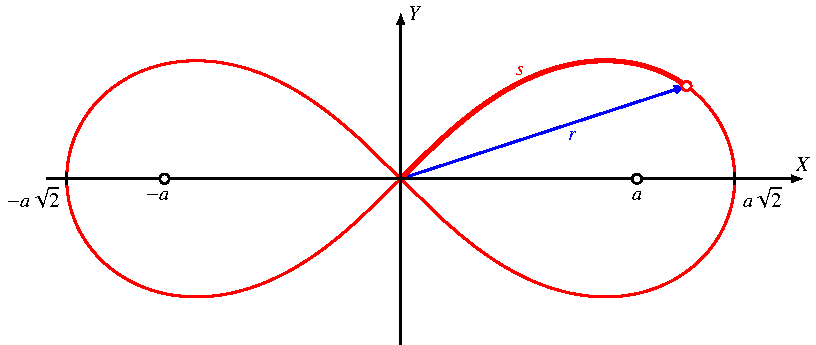
\includegraphics{chapters/110-elliptisch/images/lemniskate.pdf}
\caption{Bogenlänge und Radius der Lemniskate von Bernoulli.
\label{buch:elliptisch:fig:lemniskate}}
\end{figure}
Die Lemniskate von Bernoulli ist die Kurve vierten Grades mit der Gleichung
\begin{equation}
(X^2+Y^2)^2 = 2a^2(X^2-Y^2).
\label{buch:elliptisch:eqn:lemniskate}
\end{equation}
Sie ist in Abbildung~\ref{buch:elliptisch:fig:lemniskate}
dargestellt.
Die beiden Scheitel der Lemniskate befinden sich bei $X_s=\pm a\sqrt{2}$.
Dividiert man die Gleichung der Lemniskate durch $X_s^2=4a^4$ entsteht 
\begin{equation}
\biggl(
\biggl(\frac{X}{a\sqrt{2}}\biggr)^2
+
\biggl(\frac{Y}{a\sqrt{2}}\biggr)^2
\biggr)^2
=
2\frac{a^2}{2a^2}\biggl(
\biggl(\frac{X}{a\sqrt{2}}\biggr)^2
-
\biggl(\frac{Y}{a\sqrt{2}}\biggr)^2
\biggr).
\qquad
\Leftrightarrow
\qquad
(x^2+y^2)^2 = x^2-y^2,
\label{buch:elliptisch:eqn:lemniskatenormiert}
\end{equation}
wobei wir $x=X/a\sqrt{2}$ und $y=Y/a\sqrt{2}$ gesetzt haben.
In dieser Normierung liegen die Scheitel bei $\pm 1$.
Dies ist die Skalierung, die für die Definition des lemniskatischen
Sinus und Kosinus verwendet werden soll.

In Polarkoordinaten $x=r\cos\varphi$ und $y=r\sin\varphi$
gilt nach Einsetzen in \eqref{buch:elliptisch:eqn:lemniskatenormiert}
\begin{equation}
r^4
=
r^2(\cos^2\varphi-\sin^2\varphi)
=
r^2\cos2\varphi
\qquad\Rightarrow\qquad
r^2 = \cos 2\varphi
\label{buch:elliptisch:eqn:lemniskatepolar}
\end{equation}
als Darstellung der Lemniskate in Polardarstellung.
Sie gilt für Winkel $\varphi\in[-\frac{\pi}4,\frac{\pi}4]$ für das
rechte Blatt und $\varphi\in[\frac{3\pi}4,\frac{5\pi}4]$ für das linke
Blatt der Lemniskate.

\subsection{Bogenlänge}
Die Funktionen
\begin{equation}
x(r) = \frac{r}{\sqrt{2}}\sqrt{1+r^2},
\quad
y(r) = \frac{r}{\sqrt{2}}\sqrt{1-r^2}
\label{buch:geometrie:eqn:lemniskateparam}
\end{equation}
erfüllen
\begin{align*}
x(r)^2-y(r)^2
&=
\frac{r^2(1+r^2)}{2}-\frac{r^2(1-r^2)}{2}
\\
&
=
r^4
=
(x(r)^2 + y(r)^2)^2,
\end{align*}
sie stellen also eine Parametrisierung der Lemniskate dar.

Mit Hilfe der Parametrisierung~\eqref{buch:geometrie:eqn:lemniskateparam}
kann man die Länge $s$ des in Abbildung~\ref{buch:elliptisch:fig:lemniskate}
dargestellten Bogens der Lemniskate berechnen.
Dazu benötigt man die Ableitungen nach $r$, die man mit der Produkt- und
Kettenregel berechnen kann:
\begin{align*}
\dot{x}(r)
&=
\frac{\sqrt{1+r^2}}{\sqrt{2}}
+
\frac{r^2}{\sqrt{2}\sqrt{1+r^2}}
&&\Rightarrow&
\dot{x}(r)^2
&=
\frac{1+r^2}{2} +r^2 + \frac{r^4}{2(1+r^2)}
\\
\dot{y}(r)
&=
\frac{\sqrt{1-r^2}}{\sqrt{2}}
-
\frac{r^2}{\sqrt{2}\sqrt{1-r^2}}
&&\Rightarrow&
\dot{y}(r)^2
&=
\frac{1-r^2}{2} -r^2 + \frac{r^4}{2(1-r^2)}
\end{align*}
Die Summe der Quadrate ist
\begin{align*}
\dot{x}(r)^2 + \dot{y}(r)^2
&=
1 + r^4\frac{1-r^2+1+r^2}{2(1+r^2)(1-r^2)}
=
1+r^4\frac{2}{2(1-r^4)}
=
\frac{1-r^4+r^4}{1-r^4}
=
\frac1{1-r^4}.
\end{align*}
Durch Einsetzen in das Integral für die Bogenlänge bekommt man
\begin{equation}
s(r)
=
\int_0^r
\frac{1}{\sqrt{1-t^4}}\,dt.
\label{buch:elliptisch:eqn:lemniskatebogenlaenge}
\end{equation}

%
% Als elliptisches Integral
%
\subsection{Darstellung als elliptisches Integral}
Das unvollständige elliptische Integral erster Art mit Parameter
$k^2=-1$ oder $k=i$ ist
\[
K(r,i)
=
\int_0^x \frac{dt}{\sqrt{(1-t^2)(1-i^2 t^2)}}
=
\int_0^x \frac{dt}{\sqrt{(1-t^2)(1-(-1)t^2)}}
=
\int_0^x \frac{dt}{\sqrt{1-t^4}}
=
s(r).
\]
Der lemniskatische Sinus ist also eine Umkehrfunktion des
elliptischen Integrals erster Art für den speziellen Wert $i$ des
Parameters $k$.

Die Länge des rechten Blattes der Lemniskate wird mit $\varpi$ bezeichnet
und hat den numerischen Wert
\[
\varpi
=
2\int_0^1\sqrt{\frac{1}{1-t^4}}\,dt
=
2.6220575542.
\]
$\varpi$ ist auch als die {\em lemniskatische Konstante} bekannt.
\index{lemniskatische Konstante}%
Der Lemniskatenbogen zwischen dem Nullpunkt und $(1,0)$ hat die Länge
$\varpi/2$.

%
%  Bogenlängenparametrisierung
%
\subsection{Bogenlängenparametrisierung}
Die Lemniskate mit der Gleichung
\[
(X^2+X^2)^2=2(X^2-X^2)
\]
(der Fall $a=1$ in \eqref{buch:elliptisch:eqn:lemniskate})
kann mit Jacobischen elliptischen Funktionen
parametrisiert werden.
Dazu schreibt man
\[
\left.
\begin{aligned}
X(t)
&=
\sqrt{2}\operatorname{cn}(t,k) \operatorname{dn}(t,k)
\\
Y(t)
&=
\phantom{\sqrt{2}}
\operatorname{cn}(t,k) \operatorname{sn}(t,k)
\end{aligned}
\quad\right\}
\qquad\text{mit $k=\displaystyle\frac{1}{\sqrt{2}}$}
\]
und berechnet die beiden Seiten der definierenden Gleichung der
Lemniskate.
Zunächst ist
\begin{align*}
X(t)^2
&=
2\operatorname{cn}(t,k)^2
\operatorname{dn}(t,k)^2
\\
Y(t)^2
&=
\operatorname{cn}(t,k)^2
\operatorname{sn}(t,k)^2
\\
X(t)^2+Y(t)^2
&=
2\operatorname{cn}(t,k)^2
\bigl(
\underbrace{
\operatorname{dn}(t,k)^2
+{\textstyle\frac12}
\operatorname{sn}(t,k)^2
}_{\displaystyle =1}
\bigr)
%\\
%&
=
2\operatorname{cn}(t,k)^2
\\
X(t)^2-Y(t)^2
&=
\operatorname{cn}(t,k)^2
\bigl(
2\operatorname{dn}(t,k)^2 - \operatorname{sn}(t,k)^2
\bigr)
\\
&=
\operatorname{cn}(t,k)^2
\bigl(
2\bigl({\textstyle\frac12}+{\textstyle\frac12}\operatorname{cn}(t,k)^2\bigr)
-
\bigl(1-\operatorname{cn}(t,k)^2\bigr)
\bigr)
\\
&=
2\operatorname{cn}(t,k)^4
\\
\Rightarrow\qquad
(X(t)^2+Y(t)^2)^2
&=
4\operatorname{cn}(t,k)^4
=
2(X(t)^2-Y(t)^2).
\end{align*}
Wir zeigen jetzt, dass dies tatsächlich eine Bogenlängenparametrisierung
der Lemniskate ist.
Dazu berechnen wir die Ableitungen
\begin{align*}
\dot{X}(t)
&=
\sqrt{2}\operatorname{cn}'(t,k)\operatorname{dn}(t,k)
+
\sqrt{2}\operatorname{cn}(t,k)\operatorname{dn}'(t,k)
\\
&=
-\sqrt{2}\operatorname{sn}(t,k)\operatorname{dn}(t,k)^2
-\frac12\sqrt{2}\operatorname{sn}(t,k)\operatorname{cn}(t,k)^2
\\
&=
-\sqrt{2}\operatorname{sn}(t,k)\bigl(
1-{\textstyle\frac12}\operatorname{sn}(t,k)^2
+{\textstyle\frac12}-{\textstyle\frac12}\operatorname{sn}(u,t)^2
\bigr)
\\
&=
\sqrt{2}\operatorname{sn}(t,k)
\bigl(
{\textstyle \frac32}-\operatorname{sn}(t,k)^2
\bigr)
\\
\dot{X}(t)^2
&=
2\operatorname{sn}(t,k)^2
\bigl(
{\textstyle \frac32}-\operatorname{sn}(t,k)^2
\bigr)^2
\\
&=
{\textstyle\frac{9}{2}}\operatorname{sn}(t,k)^2
-
6\operatorname{sn}(t,k)^4
+2\operatorname{sn}(t,k)^6
\\
\dot{Y}(t)
&=
\operatorname{cn}'(t,k)\operatorname{sn}(t,k)
+
\operatorname{cn}(t,k)\operatorname{sn}'(t,k)
\\
&=
-\operatorname{sn}(t,k)^2
\operatorname{dn}(t,k)
+\operatorname{cn}(t,k)^2
\operatorname{dn}(t,k)
\\
&=
\operatorname{dn}(t,k)\bigl(1-2\operatorname{sn}(t,k)^2\bigr)
\\
\dot{Y}(t)^2
&=
\bigl(1-{\textstyle\frac12}\operatorname{sn}(t,k)^2\bigr)
\bigl(1-2\operatorname|{sn}(t,k)^2\bigr)^2
\\
&=
1-{\textstyle\frac{9}{2}}\operatorname{sn}(t,k)^2
+6\operatorname{sn}(t,k)^4
-2\operatorname{sn}(t,k)^6
\\
\dot{X}(t)^2 + \dot{Y}(t)^2
&=
1.
\end{align*}
Dies bedeutet, dass die Bogenlänge zwischen den Parameterwerten $0$ und $s$
\[
\int_0^s
\sqrt{\dot{X}(t)^2 + \dot{Y}(t)^2}
\,dt
=
\int_0^s\,dt
=
s,
\]
der Parameter $t$ ist also ein Bogenlängenparameter.

Die mit dem Faktor $1/\sqrt{2}$ skalierte Standard-Lemniskate mit der
Gleichung
\[
(x^2+y^2)^2 = x^2-y^2
\]
hat daher eine Bogenlängenparametrisierung mit
\begin{equation}
\begin{aligned}
x(t)
&=
\phantom{\frac{1}{\sqrt{2}}}
\operatorname{cn}(\sqrt{2}t,k)\operatorname{dn}(\sqrt{2}t,k)
\\
y(t)
&=
\frac{1}{\sqrt{2}}\operatorname{cn}(\sqrt{2}t,k)\operatorname{sn}(\sqrt{2}t,k)
\end{aligned}
\label{buch:elliptisch:lemniskate:bogenlaenge}
\end{equation}

\subsection{Der lemniskatische Sinus und Kosinus}
Der Sinus Berechnet die Gegenkathete zu einer gegebenen Bogenlänge des
Kreises, er ist die Umkehrfunktion der Funktion, die der Gegenkathete
die Bogenlänge zuordnet.

Daher ist es naheliegend, die Umkehrfunktion von $s(r)$ in 
\eqref{buch:elliptisch:eqn:lemniskatebogenlaenge}
den {\em lemniskatischen Sinus} zu nennen mit der Bezeichnung
$r=\operatorname{sl} s$.

Der Kosinus ist der Sinus des komplementären Winkels.
Auch für die lemniskatische Bogenlänge $s(r)$ lässt sich eine
komplementäre Bogenlänge definieren, nämlich die Bogenlänge zwischen
dem Punkt $(x(r), y(r))$ und $(1,0)$.

Da die Parametrisierung~\eqref{buch:elliptisch:lemniskate:bogenlaenge}
eine Bogenlängenparametrisierung ist, darf man $t=s$ schreiben.
Dann kann man aber auch $r(s)$ daraus berechnen,
es ist
\[
r(s)^2
=
x(s)^2 + y(s)^2
=
\operatorname{cn}(s\sqrt{2},k)^2
\qquad\Rightarrow\qquad
r(s)
=
\operatorname{cn}(s\sqrt{2},k)
\]

\begin{figure}
\centering
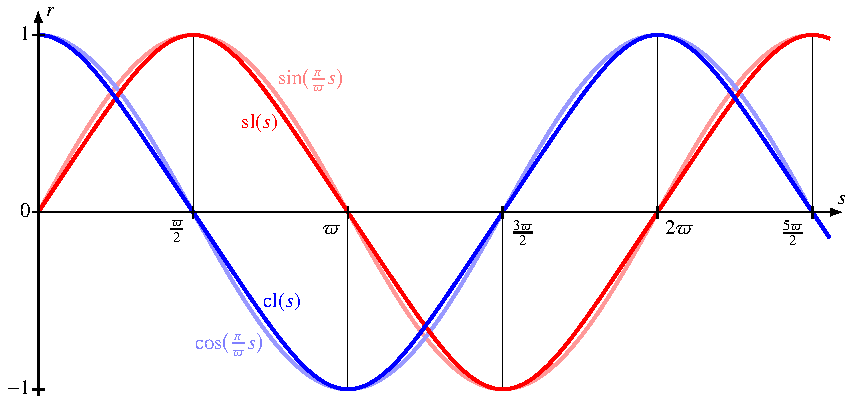
\includegraphics{chapters/110-elliptisch/images/slcl.pdf}
\caption{
Lemniskatischer Sinus und Kosinus sowie Sinus und Kosinus
mit derart skaliertem Argument, dass die Funktionen die gleichen Nullstellen
haben.
\label{buch:elliptisch:figure:slcl}}
\end{figure}


%\section*{Übungsaufgaben}
%\rhead{Übungsaufgaben}
%\aufgabetoplevel{chapters/020-exponential/uebungsaufgaben}
%\begin{uebungsaufgaben}
%\uebungsaufgabe{0}
%\uebungsaufgabe{1}
%\end{uebungsaufgaben}


%
% chapter.tex -- Beschreibung des Inhaltes
%
% (c) 2021 Prof Dr Andreas Müller, Hochschule Rapperswil
%
% !TeX spellcheck = de_CH
\chapter{Elliptische Funktionen
\label{buch:chapter:geometrie}}
\lhead{Elliptische Funktionen}
\rhead{}

Der Versuch, die Länge eines Ellipsenbogens zu berechnen, hat
in Abschnitt~\ref{buch:geometrie:subsection:hyperbeln-und-ellipsen}
zu Integralen geführt, die nicht in geschlossener Form ausgewertet
werden können.
Neben den dort gefundenen Integralen sind noch weitere, ähnlich
aufgebaute Integrale in dieser Familie zu finden.

%
% ellintegral.tex
%
% (c) 2021 Prof Dr Andreas Müller, OST Ostschweizer Fachhochschule
%
\section{Elliptische Integrale
\label{buch:elliptisch:section:integral}}
\rhead{Elliptisches Integral}
Bei der Berechnung des Ellipsenbogens in 
Abschnitt~\ref{buch:geometrie:subsection:hyperbeln-und-ellipsen}
sind wir auf ein Integral gestossen, welches sich nicht in geschlossener
Form ausdrücken liess.
Um solche Integrale in den Griff zu bekommen, ist es nötig, sie als
neue spezielle Funktionen zu definieren.

\subsection{Definition
\label{buch:elliptisch:subsection:definition}}
Ein {\em elliptisches Integral} ist ein Integral der Form
\index{elliptishes Integral}%
\index{Integral, elliptisch}%
\begin{equation}
\int R\left( x, \sqrt{p(x)}\right)\,dx
\label{buch:elliptisch:def:allgemein}
\end{equation}
wobei $R(x,y)$ eine rationale Funktion von zwei Variablen ist und
$p(x)$ ein Polynom dritten oder vierten Grades.
Hätte $p(x)$ ein mehrfache Nullstelle $x_0$, müsste es durch $(x-x_0)^2$
teilbar sein, man könnte also einen Faktor $(x-x_0)$ aus der
Wurzel im Integraneden von \eqref{buch:elliptisch:def:allgemein}
ausklammern und damit das Integral in eine Form bringen, wo $p(x)$
höchstens zweiten Grades ist.
Solche Integrale lassen sich meistens mit trigonometrischen Substitutionen
berechnen.
Wir verlangen daher, dass $p(x)$ keine mehrfachen Nullstellen hat.

Man kann zeigen, dass sich elliptische Integrale in Summen von
elementaren Funktionen und speziellen elliptischen Integralen 
der folgenden Form überführen lassen
\cite[Abschnitt 164, p.~506]{buch:smirnov32}.

\begin{definition}
\label{buch:elliptisch:def:integrale123}
Die elliptischen Integrale erster, zweiter und dritter Art sind die
Integrale
\[
\begin{aligned}
\text{1.~Art:}&&&
\int \frac{dx}{\sqrt{(1-x^2)(1-k^2x^2)}}
\\
\text{2.~Art:}&&&
\int \sqrt{\frac{1-k^2x^2}{1-x^2}}\,dx
\\
\text{3.~Art:}&&&
\int \frac{dx}{(1-nx^2)\sqrt{(1-x^2)(1-k^2x^2)}}
\end{aligned}
\]
mit $0<k<1$.
Es ist auch üblich, den Parameter $m=k^2$ zu verwenden.
\end{definition}

Wie gesagt lassen sich für diese unbestimmten Integrale keine 
geschlossenen Formen finden.
Es bleibt uns daher nichts anderes übrig, als die Integralgrenzen
festzulegen und damit eine Stammfunktion auszuwählen.

%
% Elliptisches Integral
%
\subsection{Vollständige elliptische Integrale
\label{buch:elliptisch:subsection:vollstaendig}}
In diesem Abschnitt legen wir beide Integrationsgrenzen fest und
untersuchen die entstehenenden Funktionen von den Parametern
$k$ und $n$.

\subsubsection{Definition der vollständigen elliptischen Integrale}
Da der Nenner in allen drei elliptischen Integralen eine Nullstelle
bei $\pm1$ hat, kann das Integral nur von $0$ bis $1$ erstreckt werden.

\begin{definition}
\label{buch:elliptisch:def:vollstintegrale123}
Die vollständigen elliptischen Integrale erster, zweiter und dritter
Art sind
\[
\begin{aligned}
\text{1.~Art:}&&
K(k)&=\int_0^1 \frac{dt}{\sqrt{(1-t^2)(1-k^2t^2)}} \\
\text{2.~Art:}&&
E(k)&=\int_0^1 \sqrt{\frac{1-k^2t^2}{1-t^2}}\,dt \\
\text{3.~Art:}&&
\Pi(n, k)&=\int_0^1\frac{dt}{(1-nt^2)\sqrt{(1-t^2)(1-k^2t^2)}} 
\end{aligned}
\]
mit $0<k<1$.
\end{definition}

Die Funktionen hängen stetig von $k$ ab.
Die Nullstellen des Faktors $1-k^2x^2$ liegen ausserhalb des
Integrationsintervalls und spielen daher keine Rolle.
Die Werte von $K(k)$ und $E(k)$ für $k=0$ können direkt berechnet
werden:
\begin{align*}
K(0)
=
E(0)
&=
\int_0^1 \frac{dt}{\sqrt{1-t^2}}=\frac{\pi}2.
\end{align*}
Das Integral $\Pi(n,0)$ ist etwas komplizierter.

Für $k\to 1$ ist $E(k)=1$, die Integrale $K(1)$ und $\Pi(n,1)$
sind dagegen divergent.

\subsubsection{Jacobi- und Legendre-Normalform}
Die Integrationsvariable $t$ der vollständigen elliptischen Integrale
kann durch die Substitution $t=\sin\varphi$ durch die Variable
$\varphi$ und das Integral über das Intervall $[0,1]$ durch ein
Integral über das Intervall $[0,\frac{\pi}2]$ ersetzt werden.
Mit
\[
\frac{dt}{d\varphi} = \cos\varphi = \sqrt{1-\sin^2\varphi}
\]
können die Funktionen $K(k)$, $E(k)$ und $\Pi(n,k)$ auch als
\begin{align*}
K(k)
&=
\int_0^{\frac{\pi}2}
\frac{
\sqrt{1-\sin^2\varphi}\,d\varphi
}{
\sqrt{(1-\sin^2\varphi)(1-k^2\sin^2\varphi)}
}
=
\int_0^{\frac{\pi}2}
\frac{d\varphi}{\sqrt{1-k^2\sin^2\varphi}}
\\
E(k)
&=
\int_0^{\frac{\pi}2}
\sqrt{\frac{1-k^2\sin^2\varphi}{1-\sin^2\varphi}}\sqrt{1-\sin^2\varphi}\,d\varphi
=
\int_0^{\frac{\pi}2}
\sqrt{1-k^2\sin^2\varphi}\,d\varphi
\\
\Pi(n,k)
&=
\int_0^{\frac{\pi}2}
\frac{
\sqrt{1-\sin^2\varphi}\,d\varphi
}{
(1-n\sin^2\varphi)\sqrt{(1-\sin^2\varphi)(1-k^2\sin^2\varphi)}
}
=
\int_0^{\frac{\pi}2}
\frac{
d\varphi
}{
(1-n\sin^2\varphi)\sqrt{1-k^2\sin^2\varphi}
}
\end{align*}
Diese Form wird auch die {\em Legendre-Normalform} der vollständigen 
\index{Legendre-Normalform}%
elliptischen Integrale genannt, während die Form von
Definition~\ref{buch:elliptisch:def:vollstintegrale123}
die {\em Jacobi-Normalform} heisst.
\index{Jacobi-Normalform}%

\subsubsection{Umfang einer Ellipse}
\begin{figure}
\centering
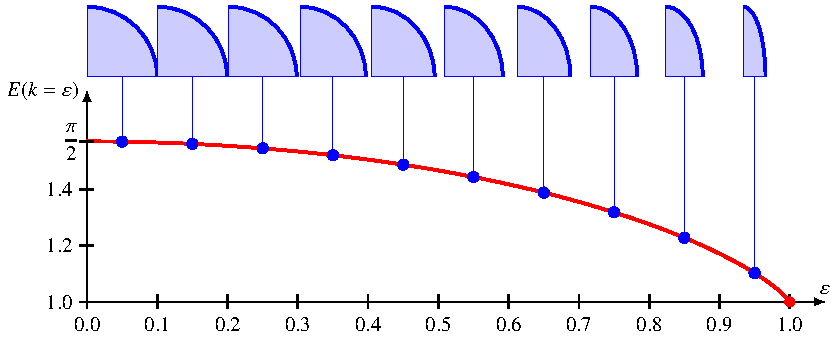
\includegraphics{chapters/110-elliptisch/images/ellipsenumfang.pdf}
\caption{Bogenlänge eines Viertels einer Ellipse mit Exzentrizität
$\varepsilon$.
\label{buch:elliptisch:fig:ellipsenumfang}}
\end{figure}
Wir zeigen, wie sich die Berechnung des Umfangs $U$ einer Ellipse
mit Halbachsen $a$ und $b$, $a\le b$, auf ein volltändiges elliptisches
Integral zurückführen lässt.
Der Fall $a>b$ kann behandelt werden, indem die $x$- und $y$-Koordinaten
vertauscht werden.

Die Parametrisierung
\[
t\mapsto \begin{pmatrix}a\cos t\\ b\sin t\end{pmatrix}
\]
einer Ellipse führt auf das Integral
\begin{align*}
U
&=
\int_0^{2\pi} \sqrt{a^2\sin^2t + b^2\cos^2 t}\,dt
\notag
\\
&=
4\int_0^{\frac{\pi}2}
\sqrt{a^2\sin^2t + b^2(1-\sin^2 t)}
\,dt
\notag
\\
&=
4b \int_0^{\frac{\pi}2} \sqrt{1-(b^2-a^2)/b^2\cdot \sin^2t}\,dt
\label{buch:elliptisch:eqn:umfangellipse}
\end{align*}
für den Umfang der Ellipse.
Bei einem Kreis ist $a=b$ und der zweite Term unter der Wurzel fällt weg,
der Umfang wird $4b\frac{\pi}2=2\pi b$.
Die Differenz $e^2=b^2-a^2$ ist die {\em lineare Exzentrizität} der Ellipse,
\index{lineare Exzentrizität}%
der Quotient $e/b$ wird die {\em numerische Exzentrizität} der Ellipse
genannt.
Insbesondere ist $k = \varepsilon$.

Das Integral~\eqref{buch:elliptisch:eqn:umfangellipse} erhält jetzt die
Form
\[
U
=
4b\int_0^{\frac{\pi}2} \sqrt{1-k^2\sin^2t}\,dt
\]
und ist damit als elliptisches Integral zweiter Art erkannt.
Für den Umfang der Ellipse finden wir damit die Formel
\[
U
=
4b E(k)
=
4b E(\varepsilon).
\]
Das vollständige elliptische Integral zweiter Art $E(\varepsilon)$
liefert also genau den Umfang der eines Viertels Ellipse mit
numerischer Exzentrizität $\varepsilon$ und kleiner Halbachse $1$.

\subsubsection{Komplementäre Integrale}
XXX Komplementäre Integrale \\

\subsubsection{Ableitung}
XXX Ableitung \\
XXX Stammfunktion \\

\subsection{Unvollständige elliptische Integrale}
XXX Vollständige und Unvollständige Integrale \\
XXX Additionstheoreme \\
XXX Parameterkonventionen \\

\subsection{Potenzreihe}
XXX Potenzreihen \\
XXX Als hypergeometrische Funktionen \\



\section{Jacobische elliptische Funktionen}

Für das elliptische Filter werden, wie es der Name bereits deutet, elliptische Funktionen gebraucht.
Wie die trigonometrischen Funktionen Zusammenhänge eines Kreises darlegen, beschreiben die elliptischen Funktionen Ellipsen.
Es ist daher naheliegend, dass der Kosinus des Tschebyscheff-Filters gegen ein elliptisches Pendant ausgetauscht werden könnte.
Der Begriff elliptische Funktion wird für sehr viele Funktionen gebraucht, daher ist es hier wichtig zu erwähnen, dass es ausschliesslich um die Jacobischen elliptischen Funktionen geht.

\subsection{Grundlegende Eigenschaften}

Die Jacobi elliptischen Funktionen werden ausführlich im Kapitel \ref{buch:elliptisch:section:jacobi} behandelt.
Im Wesentlichen erweitern die Jacobi elliptischen Funktionen die trigonometrische Funktionen für Ellipsen.
Zum Beispiel gibt es analog zum Sinus den elliptischen $\sn(z, k)$.
Im Gegensatz zum den trigonometrischen Funktionen haben die elliptischen Funktionen zwei Parameter.
Den \textit{elliptische Modul} $k$, der die Exzentrizität der Ellipse parametrisiert und das Winkelargument $z$.
Im Kreis ist der Radius für alle Winkel konstant, bei Ellipsen ändert sich das.
Dies hat zur Folge, dass bei einer Ellipse die Kreisbogenlänge nicht linear zum Winkel verläuft.
Darum kann hier nicht der gewohnte Winkel verwendet werden.
Das Winkelargument $z$ kann durch das elliptische Integral erster Art
\begin{equation}
    z
    =
    F(\phi, k)
    =
    \int_{0}^{\phi}
    \frac{
        d\theta
    }{
        \sqrt{
            1-k^2 \sin^2 \theta
        }
    }
\end{equation}
mit dem Winkel $\phi$ in Verbindung gebracht werden.

Dabei wird das vollständige und unvollständige elliptische integral unterschieden.
Beim vollständigen Integral
\begin{equation}
    K(k)
    =
    \int_{0}^{\pi / 2}
    \frac{
        d\theta
    }{
        \sqrt{
            1-k^2 \sin^2 \theta
        }
    }
\end{equation}
wird über ein viertel Ellipsenbogen integriert, also bis $\phi=\pi/2$ und liefert das Winkelargument für eine Vierteldrehung.
Die Zahl wird oft auch abgekürzt mit $K = K(k)$ und ist für das elliptische Filter sehr relevant.
Alle elliptischen Funktionen sind somit $4K$-periodisch.

Neben dem $\sn$ gibt es zwei weitere elliptische Basisfunktionen $\cn$ und $\dn$.
Dazu kommen noch weitere abgeleitete Funktionen, die durch Quotienten und Kehrwerte dieser Funktionen zustande kommen.
Insgesamt sind es die zwölf Funktionen
\begin{equation*}
    \sn \quad
    \ns \quad
    \scelliptic \quad
    \sd \quad
    \cn \quad
    \nc \quad
    \cs \quad
    \cd \quad
    \dn \quad
    \nd \quad
    \ds \quad
    \dc.
\end{equation*}

Die Jacobischen elliptischen Funktionen können mit der inversen Funktion des vollständigen elliptischen Integrals erster Art
\begin{equation}
    \phi = F^{-1}(z, k)
\end{equation}
definiert werden. Dabei ist zu beachten dass nur das $z$ Argument der Funktion invertiert wird, also
\begin{equation}
    z = F(\phi, k)
    \Leftrightarrow
    \phi = F^{-1}(z, k).
\end{equation}
Mithilfe von $F^{-1}$ kann zum Beispiel $sn^{-1}$ mit dem elliptischen Integral dargestellt werden:
\begin{equation}
    \sin(\phi)
    =
    \sin \left( F^{-1}(z, k) \right)
    =
    \sn(z, k)
    =
    w.
\end{equation}

% \begin{equation} %TODO remove unnecessary equations
%     \phi
%     =
%      F^{-1}(z, k)
%      =
%      \sin^{-1} \big( \sn (z, k ) \big)
%      =
%     \sin^{-1} ( w )
% \end{equation}

% \begin{equation}
%     F(\phi, k)
%     =
%     z
%     =
%     F( \sin^{-1} \big( \sn (z, k ) \big) , k)
%     =
%     F( \sin^{-1} ( w ), k)
% \end{equation}

% \begin{equation}
%     \sn^{-1}(w, k)
%     =
%     F(\phi, k),
%     \quad
%     \phi = \sin^{-1}(w)
% \end{equation}

\subsection{Die Funktion $\sn^{-1}$}

Beim Tschebyscheff-Filter konnten wir mit Betrachten des Arcuscosinus die Funktionalität erklären.
Für das Elliptische Filter machen wir die gleiche Betrachtung mit der $\sn^{-1}$-Funktion.
Der $\sn^{-1}$ ist durch das elliptische Integral
\begin{align}
    \sn^{-1}(w, k)
        & =
    \int_{0}^{\phi}
    \frac{
        d\theta
    }{
        \sqrt{
            1-k^2 \sin^2 \theta
        }
    },
    \quad
    \phi = \sin^{-1}(w)
    \\
        & =
    \int_{0}^{w}
    \frac{
        dt
    }{
        \sqrt{
            (1-t^2)(1-k^2 t^2)
        }
    }
\end{align}
beschrieben.
Dazu betrachten wir wieder den Integranden
\begin{equation}
    \frac{
        1
    }{
        \sqrt{
            (1-t^2)(1-k^2 t^2)
        }
    }.
\end{equation}
Beim $\cos^{-1}(x)$ haben wir gesehen, dass die analytische Fortsetzung bei $x < -1$ und $x > 1$ rechtwinklig in die komplexen Zahlen wandert.
Wenn man das Gleiche mit $\sn^{-1}(w, k)$ macht, erkennt man zwei interessante Stellen.
Die erste ist die gleiche wie beim $\cos^{-1}(x)$ nämlich bei $t = \pm 1$.
Der erste Term unter der Wurzel wird dann negativ, während der zweite noch positiv ist, da $k \leq 1$.
Ab diesem Punkt knickt die Funktion in die imaginäre Richtung ab.
Bei $t = 1/k$ ist auch der zweite Term negativ und die Funktion verläuft in die negative reelle Richtung.
Abbildung \ref{ellfilter:fig:sn} zeigt den Verlauf der Funktion in der komplexen Ebene.
\begin{figure}
    \centering
    \begin{tikzpicture}[>=stealth', auto, node distance=2cm, scale=1.2]

    \tikzstyle{zero} = [draw, circle, inner sep =0, minimum height=0.15cm]

    \tikzset{pole/.style={cross out, draw=black, minimum size=(0.15cm-\pgflinewidth), inner sep=0pt, outer sep=0pt}}

    \begin{scope}[xscale=0.9, yscale=1.8]

        \draw[gray, ->] (0,-1.5) -- (0,1.5) node[anchor=south]{$\mathrm{Im}~z$};
        \draw[gray, ->] (-5,0) -- (5,0) node[anchor=west]{$\mathrm{Re}~z$};

        \begin{scope}

            \clip(-4.5,-1.25) rectangle (4.5,1.25);

            \fill[yellow!30] (0,0) rectangle (1, 0.5);

            \begin{scope}[xshift=-1cm]

                \foreach \i in {-2,...,2} {
                    \foreach \j in {-2,...,1} {
                        \begin{scope}[xshift=\i*4cm, yshift=\j*1cm]
                            \draw[<-, blue!50] (0, 0) -- (0,0.5);
                            \draw[<-, cyan!50] (1, 0) -- (0,0);
                            \draw[<-, darkgreen!50] (2, 0) -- (1,0);
                            \draw[<-, orange!50] (2,0.5) -- (2, 0);
                            \draw[<-, red!50] (1, 0.5) -- (2,0.5);
                            \draw[<-, purple!50] (0, 0.5) -- (1,0.5);
                            \draw[<-, blue!50] (0,1) -- (0,0.5);
                            \draw[<-, orange!50] (2,0.5) -- (2, 1);
                            \draw[<-, red!50] (3, 0.5) -- (2,0.5);
                            \draw[<-, purple!50] (4, 0.5) -- (3,0.5);
                            \draw[<-, darkgreen!50] (2, 0) -- (3,0);
                            \draw[<-, cyan!50] (3, 0) -- (4,0);
                        \end{scope}
                    }
                }

                % \pause
                \draw[ultra thick, <-, darkgreen] (2, 0) -- (1,0);
                % \pause
                \draw[ultra thick, <-, orange] (2,0.5) -- (2, 0);
                % \pause
                \draw[ultra thick, <-, red] (1, 0.5) -- (2,0.5);
                % \pause
                \draw[ultra thick, <-, blue] (0, 0) -- (0,0.5);
                \draw[ultra thick, <-, purple] (0, 0.5) -- (1,0.5);
                \draw[ultra thick, <-, cyan] (1, 0) -- (0,0);
                % \pause


                \foreach \i in {-2,...,2} {
                    \foreach \j in {-2,...,1} {
                        \begin{scope}[xshift=\i*4cm, yshift=\j*1cm]
                            \node[zero] at ( 1, 0) {};
                            \node[zero] at ( 3, 0) {};
                            \node[pole] at ( 1,0.5) {};
                            \node[pole] at ( 3,0.5) {};
                        \end{scope}
                    }
                }

            \end{scope}

        \end{scope}

        \draw[gray] ( 1,0) +(0,0.1) -- +(0, -0.1) node[inner sep=0, anchor=north] {\small $K$};
        \draw[gray]  (0, 0.5) +(0.1, 0) -- +(-0.1, 0) node[inner sep=0, anchor=east]{\small $jK^\prime$};

    \end{scope}

    \node[zero] at (4,3) (n) {};
    \node[anchor=west] at (n.east) {Zero};
    \node[pole, below=0.25cm of n] (n) {};
    \node[anchor=west] at (n.east) {Pole};

    \begin{scope}[yshift=-4cm, xscale=0.75]

        \draw[gray, ->] (-6,0) -- (6,0) node[anchor=west]{$w$};

        \draw[ultra thick, ->, purple] (-5, 0) -- (-3, 0);
        \draw[ultra thick, ->, blue]      (-3, 0) -- (-2, 0);
        \draw[ultra thick, ->, cyan]       (-2, 0) -- (0, 0);
        \draw[ultra thick, ->, darkgreen]    (0, 0) -- (2, 0);
        \draw[ultra thick, ->, orange] (2, 0) -- (3, 0);
        \draw[ultra thick, ->, red] (3, 0) -- (5, 0);

        \node[anchor=south] at (-5,0) {$-\infty$};
        \node[anchor=south] at (-3,0) {$-1/k$};
        \node[anchor=south] at (-2,0) {$-1$};
        \node[anchor=south] at (0,0) {$0$};
        \node[anchor=south] at (2,0) {$1$};
        \node[anchor=south] at (3,0) {$1/k$};
        \node[anchor=south] at (5,0) {$\infty$};

    \end{scope}


\end{tikzpicture}
    \caption{
        $z$-Ebene der Funktion $z = \sn^{-1}(w, k)$.
        Die Funktion ist in der realen Achse $4K$-periodisch und in der imaginären Achse $2jK^\prime$-periodisch.
    }
    \label{ellfilter:fig:sn}
\end{figure}
In der reellen Richtung ist sie $4K(k)$-periodisch und in der imaginären Richtung $4K^\prime(k)$-periodisch, wobei $K^\prime$ das komplementäre vollständige Elliptische Integral ist:
\begin{equation}
    K^\prime(k)
    =
    \int_{0}^{\pi / 2}
    \frac{
        d\theta
    }{
        \sqrt{
            1-{k^\prime}^2 \sin^2 \theta
        }
    },
    \quad
    k^\prime = \sqrt{1-k^2}.
\end{equation}

%
% lemniskate.tex
%
% (c) 2021 Prof Dr Andreas Müller, OST Ostschweizer Fachhochschule
%
\section{Lemniskatischer Sinus
\label{buch:elliptisch:section:lemniskate}}
\rhead{Lemniskatischer Sinus}
Historisch war der {\em lemniskatische Sinus} die erste ellptische
Funktion, die Gauss bereits als 19-jähriger untersucht, aber nicht 
veröffentlich hat.
In diesem Abschnitt soll die Verbindung zu den Jacobischen
elliptischen Funktionen hergestellt werden.

\subsection{Lemniskate
\label{buch:gemotrie:subsection:lemniskate}}
\begin{figure}
\centering
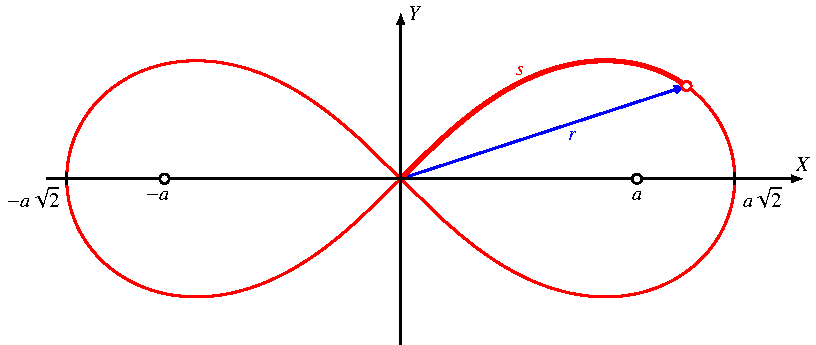
\includegraphics{chapters/110-elliptisch/images/lemniskate.pdf}
\caption{Bogenlänge und Radius der Lemniskate von Bernoulli.
\label{buch:elliptisch:fig:lemniskate}}
\end{figure}
Die Lemniskate von Bernoulli ist die Kurve vierten Grades mit der Gleichung
\begin{equation}
(X^2+Y^2)^2 = 2a^2(X^2-Y^2).
\label{buch:elliptisch:eqn:lemniskate}
\end{equation}
Sie ist in Abbildung~\ref{buch:elliptisch:fig:lemniskate}
dargestellt.
Die beiden Scheitel der Lemniskate befinden sich bei $X_s=\pm a\sqrt{2}$.
Dividiert man die Gleichung der Lemniskate durch $X_s^2=4a^4$ entsteht 
\begin{equation}
\biggl(
\biggl(\frac{X}{a\sqrt{2}}\biggr)^2
+
\biggl(\frac{Y}{a\sqrt{2}}\biggr)^2
\biggr)^2
=
2\frac{a^2}{2a^2}\biggl(
\biggl(\frac{X}{a\sqrt{2}}\biggr)^2
-
\biggl(\frac{Y}{a\sqrt{2}}\biggr)^2
\biggr).
\qquad
\Leftrightarrow
\qquad
(x^2+y^2)^2 = x^2-y^2,
\label{buch:elliptisch:eqn:lemniskatenormiert}
\end{equation}
wobei wir $x=X/a\sqrt{2}$ und $y=Y/a\sqrt{2}$ gesetzt haben.
In dieser Normierung liegen die Scheitel bei $\pm 1$.
Dies ist die Skalierung, die für die Definition des lemniskatischen
Sinus und Kosinus verwendet werden soll.

In Polarkoordinaten $x=r\cos\varphi$ und $y=r\sin\varphi$
gilt nach Einsetzen in \eqref{buch:elliptisch:eqn:lemniskatenormiert}
\begin{equation}
r^4
=
r^2(\cos^2\varphi-\sin^2\varphi)
=
r^2\cos2\varphi
\qquad\Rightarrow\qquad
r^2 = \cos 2\varphi
\label{buch:elliptisch:eqn:lemniskatepolar}
\end{equation}
als Darstellung der Lemniskate in Polardarstellung.
Sie gilt für Winkel $\varphi\in[-\frac{\pi}4,\frac{\pi}4]$ für das
rechte Blatt und $\varphi\in[\frac{3\pi}4,\frac{5\pi}4]$ für das linke
Blatt der Lemniskate.

\subsection{Bogenlänge}
Die Funktionen
\begin{equation}
x(r) = \frac{r}{\sqrt{2}}\sqrt{1+r^2},
\quad
y(r) = \frac{r}{\sqrt{2}}\sqrt{1-r^2}
\label{buch:geometrie:eqn:lemniskateparam}
\end{equation}
erfüllen
\begin{align*}
x(r)^2-y(r)^2
&=
\frac{r^2(1+r^2)}{2}-\frac{r^2(1-r^2)}{2}
\\
&
=
r^4
=
(x(r)^2 + y(r)^2)^2,
\end{align*}
sie stellen also eine Parametrisierung der Lemniskate dar.

Mit Hilfe der Parametrisierung~\eqref{buch:geometrie:eqn:lemniskateparam}
kann man die Länge $s$ des in Abbildung~\ref{buch:elliptisch:fig:lemniskate}
dargestellten Bogens der Lemniskate berechnen.
Dazu benötigt man die Ableitungen nach $r$, die man mit der Produkt- und
Kettenregel berechnen kann:
\begin{align*}
\dot{x}(r)
&=
\frac{\sqrt{1+r^2}}{\sqrt{2}}
+
\frac{r^2}{\sqrt{2}\sqrt{1+r^2}}
&&\Rightarrow&
\dot{x}(r)^2
&=
\frac{1+r^2}{2} +r^2 + \frac{r^4}{2(1+r^2)}
\\
\dot{y}(r)
&=
\frac{\sqrt{1-r^2}}{\sqrt{2}}
-
\frac{r^2}{\sqrt{2}\sqrt{1-r^2}}
&&\Rightarrow&
\dot{y}(r)^2
&=
\frac{1-r^2}{2} -r^2 + \frac{r^4}{2(1-r^2)}
\end{align*}
Die Summe der Quadrate ist
\begin{align*}
\dot{x}(r)^2 + \dot{y}(r)^2
&=
1 + r^4\frac{1-r^2+1+r^2}{2(1+r^2)(1-r^2)}
=
1+r^4\frac{2}{2(1-r^4)}
=
\frac{1-r^4+r^4}{1-r^4}
=
\frac1{1-r^4}.
\end{align*}
Durch Einsetzen in das Integral für die Bogenlänge bekommt man
\begin{equation}
s(r)
=
\int_0^r
\frac{1}{\sqrt{1-t^4}}\,dt.
\label{buch:elliptisch:eqn:lemniskatebogenlaenge}
\end{equation}

%
% Als elliptisches Integral
%
\subsection{Darstellung als elliptisches Integral}
Das unvollständige elliptische Integral erster Art mit Parameter
$k^2=-1$ oder $k=i$ ist
\[
K(r,i)
=
\int_0^x \frac{dt}{\sqrt{(1-t^2)(1-i^2 t^2)}}
=
\int_0^x \frac{dt}{\sqrt{(1-t^2)(1-(-1)t^2)}}
=
\int_0^x \frac{dt}{\sqrt{1-t^4}}
=
s(r).
\]
Der lemniskatische Sinus ist also eine Umkehrfunktion des
elliptischen Integrals erster Art für den speziellen Wert $i$ des
Parameters $k$.

Die Länge des rechten Blattes der Lemniskate wird mit $\varpi$ bezeichnet
und hat den numerischen Wert
\[
\varpi
=
2\int_0^1\sqrt{\frac{1}{1-t^4}}\,dt
=
2.6220575542.
\]
$\varpi$ ist auch als die {\em lemniskatische Konstante} bekannt.
\index{lemniskatische Konstante}%
Der Lemniskatenbogen zwischen dem Nullpunkt und $(1,0)$ hat die Länge
$\varpi/2$.

%
%  Bogenlängenparametrisierung
%
\subsection{Bogenlängenparametrisierung}
Die Lemniskate mit der Gleichung
\[
(X^2+X^2)^2=2(X^2-X^2)
\]
(der Fall $a=1$ in \eqref{buch:elliptisch:eqn:lemniskate})
kann mit Jacobischen elliptischen Funktionen
parametrisiert werden.
Dazu schreibt man
\[
\left.
\begin{aligned}
X(t)
&=
\sqrt{2}\operatorname{cn}(t,k) \operatorname{dn}(t,k)
\\
Y(t)
&=
\phantom{\sqrt{2}}
\operatorname{cn}(t,k) \operatorname{sn}(t,k)
\end{aligned}
\quad\right\}
\qquad\text{mit $k=\displaystyle\frac{1}{\sqrt{2}}$}
\]
und berechnet die beiden Seiten der definierenden Gleichung der
Lemniskate.
Zunächst ist
\begin{align*}
X(t)^2
&=
2\operatorname{cn}(t,k)^2
\operatorname{dn}(t,k)^2
\\
Y(t)^2
&=
\operatorname{cn}(t,k)^2
\operatorname{sn}(t,k)^2
\\
X(t)^2+Y(t)^2
&=
2\operatorname{cn}(t,k)^2
\bigl(
\underbrace{
\operatorname{dn}(t,k)^2
+{\textstyle\frac12}
\operatorname{sn}(t,k)^2
}_{\displaystyle =1}
\bigr)
%\\
%&
=
2\operatorname{cn}(t,k)^2
\\
X(t)^2-Y(t)^2
&=
\operatorname{cn}(t,k)^2
\bigl(
2\operatorname{dn}(t,k)^2 - \operatorname{sn}(t,k)^2
\bigr)
\\
&=
\operatorname{cn}(t,k)^2
\bigl(
2\bigl({\textstyle\frac12}+{\textstyle\frac12}\operatorname{cn}(t,k)^2\bigr)
-
\bigl(1-\operatorname{cn}(t,k)^2\bigr)
\bigr)
\\
&=
2\operatorname{cn}(t,k)^4
\\
\Rightarrow\qquad
(X(t)^2+Y(t)^2)^2
&=
4\operatorname{cn}(t,k)^4
=
2(X(t)^2-Y(t)^2).
\end{align*}
Wir zeigen jetzt, dass dies tatsächlich eine Bogenlängenparametrisierung
der Lemniskate ist.
Dazu berechnen wir die Ableitungen
\begin{align*}
\dot{X}(t)
&=
\sqrt{2}\operatorname{cn}'(t,k)\operatorname{dn}(t,k)
+
\sqrt{2}\operatorname{cn}(t,k)\operatorname{dn}'(t,k)
\\
&=
-\sqrt{2}\operatorname{sn}(t,k)\operatorname{dn}(t,k)^2
-\frac12\sqrt{2}\operatorname{sn}(t,k)\operatorname{cn}(t,k)^2
\\
&=
-\sqrt{2}\operatorname{sn}(t,k)\bigl(
1-{\textstyle\frac12}\operatorname{sn}(t,k)^2
+{\textstyle\frac12}-{\textstyle\frac12}\operatorname{sn}(u,t)^2
\bigr)
\\
&=
\sqrt{2}\operatorname{sn}(t,k)
\bigl(
{\textstyle \frac32}-\operatorname{sn}(t,k)^2
\bigr)
\\
\dot{X}(t)^2
&=
2\operatorname{sn}(t,k)^2
\bigl(
{\textstyle \frac32}-\operatorname{sn}(t,k)^2
\bigr)^2
\\
&=
{\textstyle\frac{9}{2}}\operatorname{sn}(t,k)^2
-
6\operatorname{sn}(t,k)^4
+2\operatorname{sn}(t,k)^6
\\
\dot{Y}(t)
&=
\operatorname{cn}'(t,k)\operatorname{sn}(t,k)
+
\operatorname{cn}(t,k)\operatorname{sn}'(t,k)
\\
&=
-\operatorname{sn}(t,k)^2
\operatorname{dn}(t,k)
+\operatorname{cn}(t,k)^2
\operatorname{dn}(t,k)
\\
&=
\operatorname{dn}(t,k)\bigl(1-2\operatorname{sn}(t,k)^2\bigr)
\\
\dot{Y}(t)^2
&=
\bigl(1-{\textstyle\frac12}\operatorname{sn}(t,k)^2\bigr)
\bigl(1-2\operatorname|{sn}(t,k)^2\bigr)^2
\\
&=
1-{\textstyle\frac{9}{2}}\operatorname{sn}(t,k)^2
+6\operatorname{sn}(t,k)^4
-2\operatorname{sn}(t,k)^6
\\
\dot{X}(t)^2 + \dot{Y}(t)^2
&=
1.
\end{align*}
Dies bedeutet, dass die Bogenlänge zwischen den Parameterwerten $0$ und $s$
\[
\int_0^s
\sqrt{\dot{X}(t)^2 + \dot{Y}(t)^2}
\,dt
=
\int_0^s\,dt
=
s,
\]
der Parameter $t$ ist also ein Bogenlängenparameter.

Die mit dem Faktor $1/\sqrt{2}$ skalierte Standard-Lemniskate mit der
Gleichung
\[
(x^2+y^2)^2 = x^2-y^2
\]
hat daher eine Bogenlängenparametrisierung mit
\begin{equation}
\begin{aligned}
x(t)
&=
\phantom{\frac{1}{\sqrt{2}}}
\operatorname{cn}(\sqrt{2}t,k)\operatorname{dn}(\sqrt{2}t,k)
\\
y(t)
&=
\frac{1}{\sqrt{2}}\operatorname{cn}(\sqrt{2}t,k)\operatorname{sn}(\sqrt{2}t,k)
\end{aligned}
\label{buch:elliptisch:lemniskate:bogenlaenge}
\end{equation}

\subsection{Der lemniskatische Sinus und Kosinus}
Der Sinus Berechnet die Gegenkathete zu einer gegebenen Bogenlänge des
Kreises, er ist die Umkehrfunktion der Funktion, die der Gegenkathete
die Bogenlänge zuordnet.

Daher ist es naheliegend, die Umkehrfunktion von $s(r)$ in 
\eqref{buch:elliptisch:eqn:lemniskatebogenlaenge}
den {\em lemniskatischen Sinus} zu nennen mit der Bezeichnung
$r=\operatorname{sl} s$.

Der Kosinus ist der Sinus des komplementären Winkels.
Auch für die lemniskatische Bogenlänge $s(r)$ lässt sich eine
komplementäre Bogenlänge definieren, nämlich die Bogenlänge zwischen
dem Punkt $(x(r), y(r))$ und $(1,0)$.

Da die Parametrisierung~\eqref{buch:elliptisch:lemniskate:bogenlaenge}
eine Bogenlängenparametrisierung ist, darf man $t=s$ schreiben.
Dann kann man aber auch $r(s)$ daraus berechnen,
es ist
\[
r(s)^2
=
x(s)^2 + y(s)^2
=
\operatorname{cn}(s\sqrt{2},k)^2
\qquad\Rightarrow\qquad
r(s)
=
\operatorname{cn}(s\sqrt{2},k)
\]

\begin{figure}
\centering
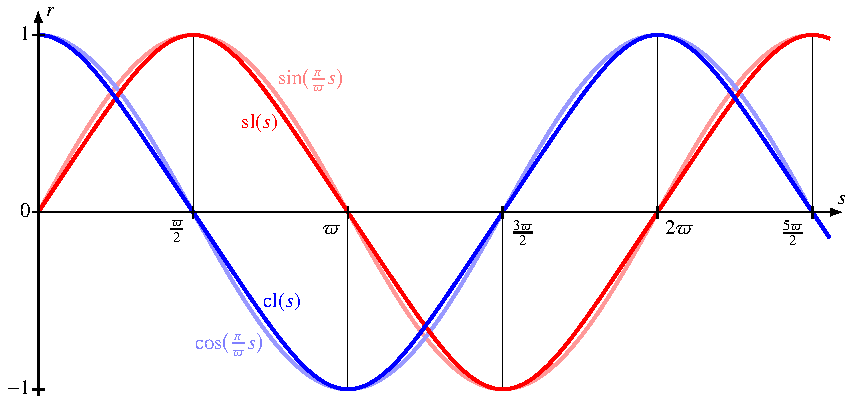
\includegraphics{chapters/110-elliptisch/images/slcl.pdf}
\caption{
Lemniskatischer Sinus und Kosinus sowie Sinus und Kosinus
mit derart skaliertem Argument, dass die Funktionen die gleichen Nullstellen
haben.
\label{buch:elliptisch:figure:slcl}}
\end{figure}


%\section*{Übungsaufgaben}
%\rhead{Übungsaufgaben}
%\aufgabetoplevel{chapters/020-exponential/uebungsaufgaben}
%\begin{uebungsaufgaben}
%\uebungsaufgabe{0}
%\uebungsaufgabe{1}
%\end{uebungsaufgaben}


%
% chapter.tex -- Beschreibung des Inhaltes
%
% (c) 2021 Prof Dr Andreas Müller, Hochschule Rapperswil
%
% !TeX spellcheck = de_CH
\chapter{Elliptische Funktionen
\label{buch:chapter:geometrie}}
\lhead{Elliptische Funktionen}
\rhead{}

Der Versuch, die Länge eines Ellipsenbogens zu berechnen, hat
in Abschnitt~\ref{buch:geometrie:subsection:hyperbeln-und-ellipsen}
zu Integralen geführt, die nicht in geschlossener Form ausgewertet
werden können.
Neben den dort gefundenen Integralen sind noch weitere, ähnlich
aufgebaute Integrale in dieser Familie zu finden.

%
% ellintegral.tex
%
% (c) 2021 Prof Dr Andreas Müller, OST Ostschweizer Fachhochschule
%
\section{Elliptische Integrale
\label{buch:elliptisch:section:integral}}
\rhead{Elliptisches Integral}
Bei der Berechnung des Ellipsenbogens in 
Abschnitt~\ref{buch:geometrie:subsection:hyperbeln-und-ellipsen}
sind wir auf ein Integral gestossen, welches sich nicht in geschlossener
Form ausdrücken liess.
Um solche Integrale in den Griff zu bekommen, ist es nötig, sie als
neue spezielle Funktionen zu definieren.

\subsection{Definition
\label{buch:elliptisch:subsection:definition}}
Ein {\em elliptisches Integral} ist ein Integral der Form
\index{elliptishes Integral}%
\index{Integral, elliptisch}%
\begin{equation}
\int R\left( x, \sqrt{p(x)}\right)\,dx
\label{buch:elliptisch:def:allgemein}
\end{equation}
wobei $R(x,y)$ eine rationale Funktion von zwei Variablen ist und
$p(x)$ ein Polynom dritten oder vierten Grades.
Hätte $p(x)$ ein mehrfache Nullstelle $x_0$, müsste es durch $(x-x_0)^2$
teilbar sein, man könnte also einen Faktor $(x-x_0)$ aus der
Wurzel im Integraneden von \eqref{buch:elliptisch:def:allgemein}
ausklammern und damit das Integral in eine Form bringen, wo $p(x)$
höchstens zweiten Grades ist.
Solche Integrale lassen sich meistens mit trigonometrischen Substitutionen
berechnen.
Wir verlangen daher, dass $p(x)$ keine mehrfachen Nullstellen hat.

Man kann zeigen, dass sich elliptische Integrale in Summen von
elementaren Funktionen und speziellen elliptischen Integralen 
der folgenden Form überführen lassen
\cite[Abschnitt 164, p.~506]{buch:smirnov32}.

\begin{definition}
\label{buch:elliptisch:def:integrale123}
Die elliptischen Integrale erster, zweiter und dritter Art sind die
Integrale
\[
\begin{aligned}
\text{1.~Art:}&&&
\int \frac{dx}{\sqrt{(1-x^2)(1-k^2x^2)}}
\\
\text{2.~Art:}&&&
\int \sqrt{\frac{1-k^2x^2}{1-x^2}}\,dx
\\
\text{3.~Art:}&&&
\int \frac{dx}{(1-nx^2)\sqrt{(1-x^2)(1-k^2x^2)}}
\end{aligned}
\]
mit $0<k<1$.
Es ist auch üblich, den Parameter $m=k^2$ zu verwenden.
\end{definition}

Wie gesagt lassen sich für diese unbestimmten Integrale keine 
geschlossenen Formen finden.
Es bleibt uns daher nichts anderes übrig, als die Integralgrenzen
festzulegen und damit eine Stammfunktion auszuwählen.

%
% Elliptisches Integral
%
\subsection{Vollständige elliptische Integrale
\label{buch:elliptisch:subsection:vollstaendig}}
In diesem Abschnitt legen wir beide Integrationsgrenzen fest und
untersuchen die entstehenenden Funktionen von den Parametern
$k$ und $n$.

\subsubsection{Definition der vollständigen elliptischen Integrale}
Da der Nenner in allen drei elliptischen Integralen eine Nullstelle
bei $\pm1$ hat, kann das Integral nur von $0$ bis $1$ erstreckt werden.

\begin{definition}
\label{buch:elliptisch:def:vollstintegrale123}
Die vollständigen elliptischen Integrale erster, zweiter und dritter
Art sind
\[
\begin{aligned}
\text{1.~Art:}&&
K(k)&=\int_0^1 \frac{dt}{\sqrt{(1-t^2)(1-k^2t^2)}} \\
\text{2.~Art:}&&
E(k)&=\int_0^1 \sqrt{\frac{1-k^2t^2}{1-t^2}}\,dt \\
\text{3.~Art:}&&
\Pi(n, k)&=\int_0^1\frac{dt}{(1-nt^2)\sqrt{(1-t^2)(1-k^2t^2)}} 
\end{aligned}
\]
mit $0<k<1$.
\end{definition}

Die Funktionen hängen stetig von $k$ ab.
Die Nullstellen des Faktors $1-k^2x^2$ liegen ausserhalb des
Integrationsintervalls und spielen daher keine Rolle.
Die Werte von $K(k)$ und $E(k)$ für $k=0$ können direkt berechnet
werden:
\begin{align*}
K(0)
=
E(0)
&=
\int_0^1 \frac{dt}{\sqrt{1-t^2}}=\frac{\pi}2.
\end{align*}
Das Integral $\Pi(n,0)$ ist etwas komplizierter.

Für $k\to 1$ ist $E(k)=1$, die Integrale $K(1)$ und $\Pi(n,1)$
sind dagegen divergent.

\subsubsection{Jacobi- und Legendre-Normalform}
Die Integrationsvariable $t$ der vollständigen elliptischen Integrale
kann durch die Substitution $t=\sin\varphi$ durch die Variable
$\varphi$ und das Integral über das Intervall $[0,1]$ durch ein
Integral über das Intervall $[0,\frac{\pi}2]$ ersetzt werden.
Mit
\[
\frac{dt}{d\varphi} = \cos\varphi = \sqrt{1-\sin^2\varphi}
\]
können die Funktionen $K(k)$, $E(k)$ und $\Pi(n,k)$ auch als
\begin{align*}
K(k)
&=
\int_0^{\frac{\pi}2}
\frac{
\sqrt{1-\sin^2\varphi}\,d\varphi
}{
\sqrt{(1-\sin^2\varphi)(1-k^2\sin^2\varphi)}
}
=
\int_0^{\frac{\pi}2}
\frac{d\varphi}{\sqrt{1-k^2\sin^2\varphi}}
\\
E(k)
&=
\int_0^{\frac{\pi}2}
\sqrt{\frac{1-k^2\sin^2\varphi}{1-\sin^2\varphi}}\sqrt{1-\sin^2\varphi}\,d\varphi
=
\int_0^{\frac{\pi}2}
\sqrt{1-k^2\sin^2\varphi}\,d\varphi
\\
\Pi(n,k)
&=
\int_0^{\frac{\pi}2}
\frac{
\sqrt{1-\sin^2\varphi}\,d\varphi
}{
(1-n\sin^2\varphi)\sqrt{(1-\sin^2\varphi)(1-k^2\sin^2\varphi)}
}
=
\int_0^{\frac{\pi}2}
\frac{
d\varphi
}{
(1-n\sin^2\varphi)\sqrt{1-k^2\sin^2\varphi}
}
\end{align*}
Diese Form wird auch die {\em Legendre-Normalform} der vollständigen 
\index{Legendre-Normalform}%
elliptischen Integrale genannt, während die Form von
Definition~\ref{buch:elliptisch:def:vollstintegrale123}
die {\em Jacobi-Normalform} heisst.
\index{Jacobi-Normalform}%

\subsubsection{Umfang einer Ellipse}
\begin{figure}
\centering
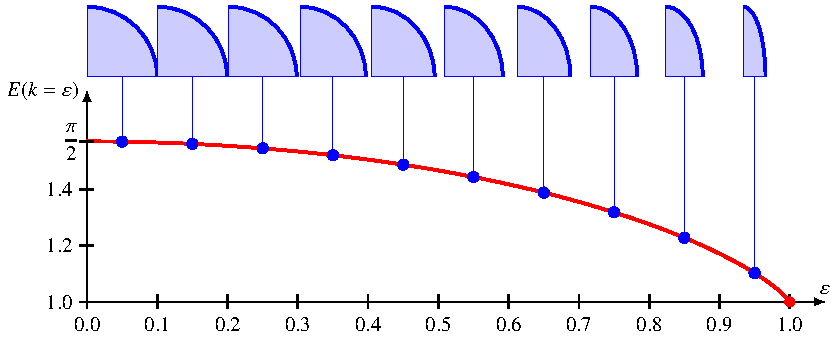
\includegraphics{chapters/110-elliptisch/images/ellipsenumfang.pdf}
\caption{Bogenlänge eines Viertels einer Ellipse mit Exzentrizität
$\varepsilon$.
\label{buch:elliptisch:fig:ellipsenumfang}}
\end{figure}
Wir zeigen, wie sich die Berechnung des Umfangs $U$ einer Ellipse
mit Halbachsen $a$ und $b$, $a\le b$, auf ein volltändiges elliptisches
Integral zurückführen lässt.
Der Fall $a>b$ kann behandelt werden, indem die $x$- und $y$-Koordinaten
vertauscht werden.

Die Parametrisierung
\[
t\mapsto \begin{pmatrix}a\cos t\\ b\sin t\end{pmatrix}
\]
einer Ellipse führt auf das Integral
\begin{align*}
U
&=
\int_0^{2\pi} \sqrt{a^2\sin^2t + b^2\cos^2 t}\,dt
\notag
\\
&=
4\int_0^{\frac{\pi}2}
\sqrt{a^2\sin^2t + b^2(1-\sin^2 t)}
\,dt
\notag
\\
&=
4b \int_0^{\frac{\pi}2} \sqrt{1-(b^2-a^2)/b^2\cdot \sin^2t}\,dt
\label{buch:elliptisch:eqn:umfangellipse}
\end{align*}
für den Umfang der Ellipse.
Bei einem Kreis ist $a=b$ und der zweite Term unter der Wurzel fällt weg,
der Umfang wird $4b\frac{\pi}2=2\pi b$.
Die Differenz $e^2=b^2-a^2$ ist die {\em lineare Exzentrizität} der Ellipse,
\index{lineare Exzentrizität}%
der Quotient $e/b$ wird die {\em numerische Exzentrizität} der Ellipse
genannt.
Insbesondere ist $k = \varepsilon$.

Das Integral~\eqref{buch:elliptisch:eqn:umfangellipse} erhält jetzt die
Form
\[
U
=
4b\int_0^{\frac{\pi}2} \sqrt{1-k^2\sin^2t}\,dt
\]
und ist damit als elliptisches Integral zweiter Art erkannt.
Für den Umfang der Ellipse finden wir damit die Formel
\[
U
=
4b E(k)
=
4b E(\varepsilon).
\]
Das vollständige elliptische Integral zweiter Art $E(\varepsilon)$
liefert also genau den Umfang der eines Viertels Ellipse mit
numerischer Exzentrizität $\varepsilon$ und kleiner Halbachse $1$.

\subsubsection{Komplementäre Integrale}
XXX Komplementäre Integrale \\

\subsubsection{Ableitung}
XXX Ableitung \\
XXX Stammfunktion \\

\subsection{Unvollständige elliptische Integrale}
XXX Vollständige und Unvollständige Integrale \\
XXX Additionstheoreme \\
XXX Parameterkonventionen \\

\subsection{Potenzreihe}
XXX Potenzreihen \\
XXX Als hypergeometrische Funktionen \\



\section{Jacobische elliptische Funktionen}

Für das elliptische Filter werden, wie es der Name bereits deutet, elliptische Funktionen gebraucht.
Wie die trigonometrischen Funktionen Zusammenhänge eines Kreises darlegen, beschreiben die elliptischen Funktionen Ellipsen.
Es ist daher naheliegend, dass der Kosinus des Tschebyscheff-Filters gegen ein elliptisches Pendant ausgetauscht werden könnte.
Der Begriff elliptische Funktion wird für sehr viele Funktionen gebraucht, daher ist es hier wichtig zu erwähnen, dass es ausschliesslich um die Jacobischen elliptischen Funktionen geht.

\subsection{Grundlegende Eigenschaften}

Die Jacobi elliptischen Funktionen werden ausführlich im Kapitel \ref{buch:elliptisch:section:jacobi} behandelt.
Im Wesentlichen erweitern die Jacobi elliptischen Funktionen die trigonometrische Funktionen für Ellipsen.
Zum Beispiel gibt es analog zum Sinus den elliptischen $\sn(z, k)$.
Im Gegensatz zum den trigonometrischen Funktionen haben die elliptischen Funktionen zwei Parameter.
Den \textit{elliptische Modul} $k$, der die Exzentrizität der Ellipse parametrisiert und das Winkelargument $z$.
Im Kreis ist der Radius für alle Winkel konstant, bei Ellipsen ändert sich das.
Dies hat zur Folge, dass bei einer Ellipse die Kreisbogenlänge nicht linear zum Winkel verläuft.
Darum kann hier nicht der gewohnte Winkel verwendet werden.
Das Winkelargument $z$ kann durch das elliptische Integral erster Art
\begin{equation}
    z
    =
    F(\phi, k)
    =
    \int_{0}^{\phi}
    \frac{
        d\theta
    }{
        \sqrt{
            1-k^2 \sin^2 \theta
        }
    }
\end{equation}
mit dem Winkel $\phi$ in Verbindung gebracht werden.

Dabei wird das vollständige und unvollständige elliptische integral unterschieden.
Beim vollständigen Integral
\begin{equation}
    K(k)
    =
    \int_{0}^{\pi / 2}
    \frac{
        d\theta
    }{
        \sqrt{
            1-k^2 \sin^2 \theta
        }
    }
\end{equation}
wird über ein viertel Ellipsenbogen integriert, also bis $\phi=\pi/2$ und liefert das Winkelargument für eine Vierteldrehung.
Die Zahl wird oft auch abgekürzt mit $K = K(k)$ und ist für das elliptische Filter sehr relevant.
Alle elliptischen Funktionen sind somit $4K$-periodisch.

Neben dem $\sn$ gibt es zwei weitere elliptische Basisfunktionen $\cn$ und $\dn$.
Dazu kommen noch weitere abgeleitete Funktionen, die durch Quotienten und Kehrwerte dieser Funktionen zustande kommen.
Insgesamt sind es die zwölf Funktionen
\begin{equation*}
    \sn \quad
    \ns \quad
    \scelliptic \quad
    \sd \quad
    \cn \quad
    \nc \quad
    \cs \quad
    \cd \quad
    \dn \quad
    \nd \quad
    \ds \quad
    \dc.
\end{equation*}

Die Jacobischen elliptischen Funktionen können mit der inversen Funktion des vollständigen elliptischen Integrals erster Art
\begin{equation}
    \phi = F^{-1}(z, k)
\end{equation}
definiert werden. Dabei ist zu beachten dass nur das $z$ Argument der Funktion invertiert wird, also
\begin{equation}
    z = F(\phi, k)
    \Leftrightarrow
    \phi = F^{-1}(z, k).
\end{equation}
Mithilfe von $F^{-1}$ kann zum Beispiel $sn^{-1}$ mit dem elliptischen Integral dargestellt werden:
\begin{equation}
    \sin(\phi)
    =
    \sin \left( F^{-1}(z, k) \right)
    =
    \sn(z, k)
    =
    w.
\end{equation}

% \begin{equation} %TODO remove unnecessary equations
%     \phi
%     =
%      F^{-1}(z, k)
%      =
%      \sin^{-1} \big( \sn (z, k ) \big)
%      =
%     \sin^{-1} ( w )
% \end{equation}

% \begin{equation}
%     F(\phi, k)
%     =
%     z
%     =
%     F( \sin^{-1} \big( \sn (z, k ) \big) , k)
%     =
%     F( \sin^{-1} ( w ), k)
% \end{equation}

% \begin{equation}
%     \sn^{-1}(w, k)
%     =
%     F(\phi, k),
%     \quad
%     \phi = \sin^{-1}(w)
% \end{equation}

\subsection{Die Funktion $\sn^{-1}$}

Beim Tschebyscheff-Filter konnten wir mit Betrachten des Arcuscosinus die Funktionalität erklären.
Für das Elliptische Filter machen wir die gleiche Betrachtung mit der $\sn^{-1}$-Funktion.
Der $\sn^{-1}$ ist durch das elliptische Integral
\begin{align}
    \sn^{-1}(w, k)
        & =
    \int_{0}^{\phi}
    \frac{
        d\theta
    }{
        \sqrt{
            1-k^2 \sin^2 \theta
        }
    },
    \quad
    \phi = \sin^{-1}(w)
    \\
        & =
    \int_{0}^{w}
    \frac{
        dt
    }{
        \sqrt{
            (1-t^2)(1-k^2 t^2)
        }
    }
\end{align}
beschrieben.
Dazu betrachten wir wieder den Integranden
\begin{equation}
    \frac{
        1
    }{
        \sqrt{
            (1-t^2)(1-k^2 t^2)
        }
    }.
\end{equation}
Beim $\cos^{-1}(x)$ haben wir gesehen, dass die analytische Fortsetzung bei $x < -1$ und $x > 1$ rechtwinklig in die komplexen Zahlen wandert.
Wenn man das Gleiche mit $\sn^{-1}(w, k)$ macht, erkennt man zwei interessante Stellen.
Die erste ist die gleiche wie beim $\cos^{-1}(x)$ nämlich bei $t = \pm 1$.
Der erste Term unter der Wurzel wird dann negativ, während der zweite noch positiv ist, da $k \leq 1$.
Ab diesem Punkt knickt die Funktion in die imaginäre Richtung ab.
Bei $t = 1/k$ ist auch der zweite Term negativ und die Funktion verläuft in die negative reelle Richtung.
Abbildung \ref{ellfilter:fig:sn} zeigt den Verlauf der Funktion in der komplexen Ebene.
\begin{figure}
    \centering
    \begin{tikzpicture}[>=stealth', auto, node distance=2cm, scale=1.2]

    \tikzstyle{zero} = [draw, circle, inner sep =0, minimum height=0.15cm]

    \tikzset{pole/.style={cross out, draw=black, minimum size=(0.15cm-\pgflinewidth), inner sep=0pt, outer sep=0pt}}

    \begin{scope}[xscale=0.9, yscale=1.8]

        \draw[gray, ->] (0,-1.5) -- (0,1.5) node[anchor=south]{$\mathrm{Im}~z$};
        \draw[gray, ->] (-5,0) -- (5,0) node[anchor=west]{$\mathrm{Re}~z$};

        \begin{scope}

            \clip(-4.5,-1.25) rectangle (4.5,1.25);

            \fill[yellow!30] (0,0) rectangle (1, 0.5);

            \begin{scope}[xshift=-1cm]

                \foreach \i in {-2,...,2} {
                    \foreach \j in {-2,...,1} {
                        \begin{scope}[xshift=\i*4cm, yshift=\j*1cm]
                            \draw[<-, blue!50] (0, 0) -- (0,0.5);
                            \draw[<-, cyan!50] (1, 0) -- (0,0);
                            \draw[<-, darkgreen!50] (2, 0) -- (1,0);
                            \draw[<-, orange!50] (2,0.5) -- (2, 0);
                            \draw[<-, red!50] (1, 0.5) -- (2,0.5);
                            \draw[<-, purple!50] (0, 0.5) -- (1,0.5);
                            \draw[<-, blue!50] (0,1) -- (0,0.5);
                            \draw[<-, orange!50] (2,0.5) -- (2, 1);
                            \draw[<-, red!50] (3, 0.5) -- (2,0.5);
                            \draw[<-, purple!50] (4, 0.5) -- (3,0.5);
                            \draw[<-, darkgreen!50] (2, 0) -- (3,0);
                            \draw[<-, cyan!50] (3, 0) -- (4,0);
                        \end{scope}
                    }
                }

                % \pause
                \draw[ultra thick, <-, darkgreen] (2, 0) -- (1,0);
                % \pause
                \draw[ultra thick, <-, orange] (2,0.5) -- (2, 0);
                % \pause
                \draw[ultra thick, <-, red] (1, 0.5) -- (2,0.5);
                % \pause
                \draw[ultra thick, <-, blue] (0, 0) -- (0,0.5);
                \draw[ultra thick, <-, purple] (0, 0.5) -- (1,0.5);
                \draw[ultra thick, <-, cyan] (1, 0) -- (0,0);
                % \pause


                \foreach \i in {-2,...,2} {
                    \foreach \j in {-2,...,1} {
                        \begin{scope}[xshift=\i*4cm, yshift=\j*1cm]
                            \node[zero] at ( 1, 0) {};
                            \node[zero] at ( 3, 0) {};
                            \node[pole] at ( 1,0.5) {};
                            \node[pole] at ( 3,0.5) {};
                        \end{scope}
                    }
                }

            \end{scope}

        \end{scope}

        \draw[gray] ( 1,0) +(0,0.1) -- +(0, -0.1) node[inner sep=0, anchor=north] {\small $K$};
        \draw[gray]  (0, 0.5) +(0.1, 0) -- +(-0.1, 0) node[inner sep=0, anchor=east]{\small $jK^\prime$};

    \end{scope}

    \node[zero] at (4,3) (n) {};
    \node[anchor=west] at (n.east) {Zero};
    \node[pole, below=0.25cm of n] (n) {};
    \node[anchor=west] at (n.east) {Pole};

    \begin{scope}[yshift=-4cm, xscale=0.75]

        \draw[gray, ->] (-6,0) -- (6,0) node[anchor=west]{$w$};

        \draw[ultra thick, ->, purple] (-5, 0) -- (-3, 0);
        \draw[ultra thick, ->, blue]      (-3, 0) -- (-2, 0);
        \draw[ultra thick, ->, cyan]       (-2, 0) -- (0, 0);
        \draw[ultra thick, ->, darkgreen]    (0, 0) -- (2, 0);
        \draw[ultra thick, ->, orange] (2, 0) -- (3, 0);
        \draw[ultra thick, ->, red] (3, 0) -- (5, 0);

        \node[anchor=south] at (-5,0) {$-\infty$};
        \node[anchor=south] at (-3,0) {$-1/k$};
        \node[anchor=south] at (-2,0) {$-1$};
        \node[anchor=south] at (0,0) {$0$};
        \node[anchor=south] at (2,0) {$1$};
        \node[anchor=south] at (3,0) {$1/k$};
        \node[anchor=south] at (5,0) {$\infty$};

    \end{scope}


\end{tikzpicture}
    \caption{
        $z$-Ebene der Funktion $z = \sn^{-1}(w, k)$.
        Die Funktion ist in der realen Achse $4K$-periodisch und in der imaginären Achse $2jK^\prime$-periodisch.
    }
    \label{ellfilter:fig:sn}
\end{figure}
In der reellen Richtung ist sie $4K(k)$-periodisch und in der imaginären Richtung $4K^\prime(k)$-periodisch, wobei $K^\prime$ das komplementäre vollständige Elliptische Integral ist:
\begin{equation}
    K^\prime(k)
    =
    \int_{0}^{\pi / 2}
    \frac{
        d\theta
    }{
        \sqrt{
            1-{k^\prime}^2 \sin^2 \theta
        }
    },
    \quad
    k^\prime = \sqrt{1-k^2}.
\end{equation}

%
% lemniskate.tex
%
% (c) 2021 Prof Dr Andreas Müller, OST Ostschweizer Fachhochschule
%
\section{Lemniskatischer Sinus
\label{buch:elliptisch:section:lemniskate}}
\rhead{Lemniskatischer Sinus}
Historisch war der {\em lemniskatische Sinus} die erste ellptische
Funktion, die Gauss bereits als 19-jähriger untersucht, aber nicht 
veröffentlich hat.
In diesem Abschnitt soll die Verbindung zu den Jacobischen
elliptischen Funktionen hergestellt werden.

\subsection{Lemniskate
\label{buch:gemotrie:subsection:lemniskate}}
\begin{figure}
\centering
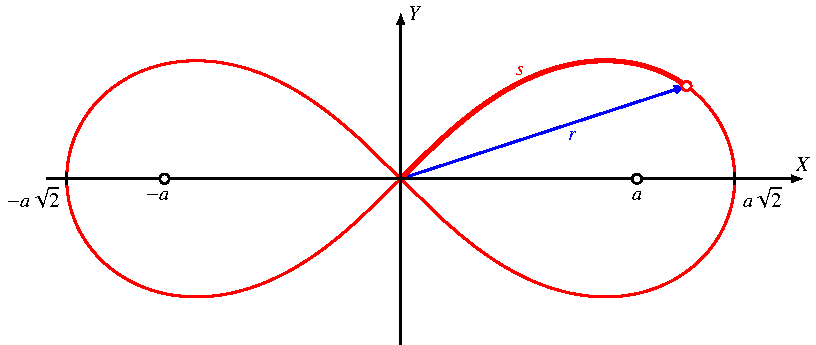
\includegraphics{chapters/110-elliptisch/images/lemniskate.pdf}
\caption{Bogenlänge und Radius der Lemniskate von Bernoulli.
\label{buch:elliptisch:fig:lemniskate}}
\end{figure}
Die Lemniskate von Bernoulli ist die Kurve vierten Grades mit der Gleichung
\begin{equation}
(X^2+Y^2)^2 = 2a^2(X^2-Y^2).
\label{buch:elliptisch:eqn:lemniskate}
\end{equation}
Sie ist in Abbildung~\ref{buch:elliptisch:fig:lemniskate}
dargestellt.
Die beiden Scheitel der Lemniskate befinden sich bei $X_s=\pm a\sqrt{2}$.
Dividiert man die Gleichung der Lemniskate durch $X_s^2=4a^4$ entsteht 
\begin{equation}
\biggl(
\biggl(\frac{X}{a\sqrt{2}}\biggr)^2
+
\biggl(\frac{Y}{a\sqrt{2}}\biggr)^2
\biggr)^2
=
2\frac{a^2}{2a^2}\biggl(
\biggl(\frac{X}{a\sqrt{2}}\biggr)^2
-
\biggl(\frac{Y}{a\sqrt{2}}\biggr)^2
\biggr).
\qquad
\Leftrightarrow
\qquad
(x^2+y^2)^2 = x^2-y^2,
\label{buch:elliptisch:eqn:lemniskatenormiert}
\end{equation}
wobei wir $x=X/a\sqrt{2}$ und $y=Y/a\sqrt{2}$ gesetzt haben.
In dieser Normierung liegen die Scheitel bei $\pm 1$.
Dies ist die Skalierung, die für die Definition des lemniskatischen
Sinus und Kosinus verwendet werden soll.

In Polarkoordinaten $x=r\cos\varphi$ und $y=r\sin\varphi$
gilt nach Einsetzen in \eqref{buch:elliptisch:eqn:lemniskatenormiert}
\begin{equation}
r^4
=
r^2(\cos^2\varphi-\sin^2\varphi)
=
r^2\cos2\varphi
\qquad\Rightarrow\qquad
r^2 = \cos 2\varphi
\label{buch:elliptisch:eqn:lemniskatepolar}
\end{equation}
als Darstellung der Lemniskate in Polardarstellung.
Sie gilt für Winkel $\varphi\in[-\frac{\pi}4,\frac{\pi}4]$ für das
rechte Blatt und $\varphi\in[\frac{3\pi}4,\frac{5\pi}4]$ für das linke
Blatt der Lemniskate.

\subsection{Bogenlänge}
Die Funktionen
\begin{equation}
x(r) = \frac{r}{\sqrt{2}}\sqrt{1+r^2},
\quad
y(r) = \frac{r}{\sqrt{2}}\sqrt{1-r^2}
\label{buch:geometrie:eqn:lemniskateparam}
\end{equation}
erfüllen
\begin{align*}
x(r)^2-y(r)^2
&=
\frac{r^2(1+r^2)}{2}-\frac{r^2(1-r^2)}{2}
\\
&
=
r^4
=
(x(r)^2 + y(r)^2)^2,
\end{align*}
sie stellen also eine Parametrisierung der Lemniskate dar.

Mit Hilfe der Parametrisierung~\eqref{buch:geometrie:eqn:lemniskateparam}
kann man die Länge $s$ des in Abbildung~\ref{buch:elliptisch:fig:lemniskate}
dargestellten Bogens der Lemniskate berechnen.
Dazu benötigt man die Ableitungen nach $r$, die man mit der Produkt- und
Kettenregel berechnen kann:
\begin{align*}
\dot{x}(r)
&=
\frac{\sqrt{1+r^2}}{\sqrt{2}}
+
\frac{r^2}{\sqrt{2}\sqrt{1+r^2}}
&&\Rightarrow&
\dot{x}(r)^2
&=
\frac{1+r^2}{2} +r^2 + \frac{r^4}{2(1+r^2)}
\\
\dot{y}(r)
&=
\frac{\sqrt{1-r^2}}{\sqrt{2}}
-
\frac{r^2}{\sqrt{2}\sqrt{1-r^2}}
&&\Rightarrow&
\dot{y}(r)^2
&=
\frac{1-r^2}{2} -r^2 + \frac{r^4}{2(1-r^2)}
\end{align*}
Die Summe der Quadrate ist
\begin{align*}
\dot{x}(r)^2 + \dot{y}(r)^2
&=
1 + r^4\frac{1-r^2+1+r^2}{2(1+r^2)(1-r^2)}
=
1+r^4\frac{2}{2(1-r^4)}
=
\frac{1-r^4+r^4}{1-r^4}
=
\frac1{1-r^4}.
\end{align*}
Durch Einsetzen in das Integral für die Bogenlänge bekommt man
\begin{equation}
s(r)
=
\int_0^r
\frac{1}{\sqrt{1-t^4}}\,dt.
\label{buch:elliptisch:eqn:lemniskatebogenlaenge}
\end{equation}

%
% Als elliptisches Integral
%
\subsection{Darstellung als elliptisches Integral}
Das unvollständige elliptische Integral erster Art mit Parameter
$k^2=-1$ oder $k=i$ ist
\[
K(r,i)
=
\int_0^x \frac{dt}{\sqrt{(1-t^2)(1-i^2 t^2)}}
=
\int_0^x \frac{dt}{\sqrt{(1-t^2)(1-(-1)t^2)}}
=
\int_0^x \frac{dt}{\sqrt{1-t^4}}
=
s(r).
\]
Der lemniskatische Sinus ist also eine Umkehrfunktion des
elliptischen Integrals erster Art für den speziellen Wert $i$ des
Parameters $k$.

Die Länge des rechten Blattes der Lemniskate wird mit $\varpi$ bezeichnet
und hat den numerischen Wert
\[
\varpi
=
2\int_0^1\sqrt{\frac{1}{1-t^4}}\,dt
=
2.6220575542.
\]
$\varpi$ ist auch als die {\em lemniskatische Konstante} bekannt.
\index{lemniskatische Konstante}%
Der Lemniskatenbogen zwischen dem Nullpunkt und $(1,0)$ hat die Länge
$\varpi/2$.

%
%  Bogenlängenparametrisierung
%
\subsection{Bogenlängenparametrisierung}
Die Lemniskate mit der Gleichung
\[
(X^2+X^2)^2=2(X^2-X^2)
\]
(der Fall $a=1$ in \eqref{buch:elliptisch:eqn:lemniskate})
kann mit Jacobischen elliptischen Funktionen
parametrisiert werden.
Dazu schreibt man
\[
\left.
\begin{aligned}
X(t)
&=
\sqrt{2}\operatorname{cn}(t,k) \operatorname{dn}(t,k)
\\
Y(t)
&=
\phantom{\sqrt{2}}
\operatorname{cn}(t,k) \operatorname{sn}(t,k)
\end{aligned}
\quad\right\}
\qquad\text{mit $k=\displaystyle\frac{1}{\sqrt{2}}$}
\]
und berechnet die beiden Seiten der definierenden Gleichung der
Lemniskate.
Zunächst ist
\begin{align*}
X(t)^2
&=
2\operatorname{cn}(t,k)^2
\operatorname{dn}(t,k)^2
\\
Y(t)^2
&=
\operatorname{cn}(t,k)^2
\operatorname{sn}(t,k)^2
\\
X(t)^2+Y(t)^2
&=
2\operatorname{cn}(t,k)^2
\bigl(
\underbrace{
\operatorname{dn}(t,k)^2
+{\textstyle\frac12}
\operatorname{sn}(t,k)^2
}_{\displaystyle =1}
\bigr)
%\\
%&
=
2\operatorname{cn}(t,k)^2
\\
X(t)^2-Y(t)^2
&=
\operatorname{cn}(t,k)^2
\bigl(
2\operatorname{dn}(t,k)^2 - \operatorname{sn}(t,k)^2
\bigr)
\\
&=
\operatorname{cn}(t,k)^2
\bigl(
2\bigl({\textstyle\frac12}+{\textstyle\frac12}\operatorname{cn}(t,k)^2\bigr)
-
\bigl(1-\operatorname{cn}(t,k)^2\bigr)
\bigr)
\\
&=
2\operatorname{cn}(t,k)^4
\\
\Rightarrow\qquad
(X(t)^2+Y(t)^2)^2
&=
4\operatorname{cn}(t,k)^4
=
2(X(t)^2-Y(t)^2).
\end{align*}
Wir zeigen jetzt, dass dies tatsächlich eine Bogenlängenparametrisierung
der Lemniskate ist.
Dazu berechnen wir die Ableitungen
\begin{align*}
\dot{X}(t)
&=
\sqrt{2}\operatorname{cn}'(t,k)\operatorname{dn}(t,k)
+
\sqrt{2}\operatorname{cn}(t,k)\operatorname{dn}'(t,k)
\\
&=
-\sqrt{2}\operatorname{sn}(t,k)\operatorname{dn}(t,k)^2
-\frac12\sqrt{2}\operatorname{sn}(t,k)\operatorname{cn}(t,k)^2
\\
&=
-\sqrt{2}\operatorname{sn}(t,k)\bigl(
1-{\textstyle\frac12}\operatorname{sn}(t,k)^2
+{\textstyle\frac12}-{\textstyle\frac12}\operatorname{sn}(u,t)^2
\bigr)
\\
&=
\sqrt{2}\operatorname{sn}(t,k)
\bigl(
{\textstyle \frac32}-\operatorname{sn}(t,k)^2
\bigr)
\\
\dot{X}(t)^2
&=
2\operatorname{sn}(t,k)^2
\bigl(
{\textstyle \frac32}-\operatorname{sn}(t,k)^2
\bigr)^2
\\
&=
{\textstyle\frac{9}{2}}\operatorname{sn}(t,k)^2
-
6\operatorname{sn}(t,k)^4
+2\operatorname{sn}(t,k)^6
\\
\dot{Y}(t)
&=
\operatorname{cn}'(t,k)\operatorname{sn}(t,k)
+
\operatorname{cn}(t,k)\operatorname{sn}'(t,k)
\\
&=
-\operatorname{sn}(t,k)^2
\operatorname{dn}(t,k)
+\operatorname{cn}(t,k)^2
\operatorname{dn}(t,k)
\\
&=
\operatorname{dn}(t,k)\bigl(1-2\operatorname{sn}(t,k)^2\bigr)
\\
\dot{Y}(t)^2
&=
\bigl(1-{\textstyle\frac12}\operatorname{sn}(t,k)^2\bigr)
\bigl(1-2\operatorname|{sn}(t,k)^2\bigr)^2
\\
&=
1-{\textstyle\frac{9}{2}}\operatorname{sn}(t,k)^2
+6\operatorname{sn}(t,k)^4
-2\operatorname{sn}(t,k)^6
\\
\dot{X}(t)^2 + \dot{Y}(t)^2
&=
1.
\end{align*}
Dies bedeutet, dass die Bogenlänge zwischen den Parameterwerten $0$ und $s$
\[
\int_0^s
\sqrt{\dot{X}(t)^2 + \dot{Y}(t)^2}
\,dt
=
\int_0^s\,dt
=
s,
\]
der Parameter $t$ ist also ein Bogenlängenparameter.

Die mit dem Faktor $1/\sqrt{2}$ skalierte Standard-Lemniskate mit der
Gleichung
\[
(x^2+y^2)^2 = x^2-y^2
\]
hat daher eine Bogenlängenparametrisierung mit
\begin{equation}
\begin{aligned}
x(t)
&=
\phantom{\frac{1}{\sqrt{2}}}
\operatorname{cn}(\sqrt{2}t,k)\operatorname{dn}(\sqrt{2}t,k)
\\
y(t)
&=
\frac{1}{\sqrt{2}}\operatorname{cn}(\sqrt{2}t,k)\operatorname{sn}(\sqrt{2}t,k)
\end{aligned}
\label{buch:elliptisch:lemniskate:bogenlaenge}
\end{equation}

\subsection{Der lemniskatische Sinus und Kosinus}
Der Sinus Berechnet die Gegenkathete zu einer gegebenen Bogenlänge des
Kreises, er ist die Umkehrfunktion der Funktion, die der Gegenkathete
die Bogenlänge zuordnet.

Daher ist es naheliegend, die Umkehrfunktion von $s(r)$ in 
\eqref{buch:elliptisch:eqn:lemniskatebogenlaenge}
den {\em lemniskatischen Sinus} zu nennen mit der Bezeichnung
$r=\operatorname{sl} s$.

Der Kosinus ist der Sinus des komplementären Winkels.
Auch für die lemniskatische Bogenlänge $s(r)$ lässt sich eine
komplementäre Bogenlänge definieren, nämlich die Bogenlänge zwischen
dem Punkt $(x(r), y(r))$ und $(1,0)$.

Da die Parametrisierung~\eqref{buch:elliptisch:lemniskate:bogenlaenge}
eine Bogenlängenparametrisierung ist, darf man $t=s$ schreiben.
Dann kann man aber auch $r(s)$ daraus berechnen,
es ist
\[
r(s)^2
=
x(s)^2 + y(s)^2
=
\operatorname{cn}(s\sqrt{2},k)^2
\qquad\Rightarrow\qquad
r(s)
=
\operatorname{cn}(s\sqrt{2},k)
\]

\begin{figure}
\centering
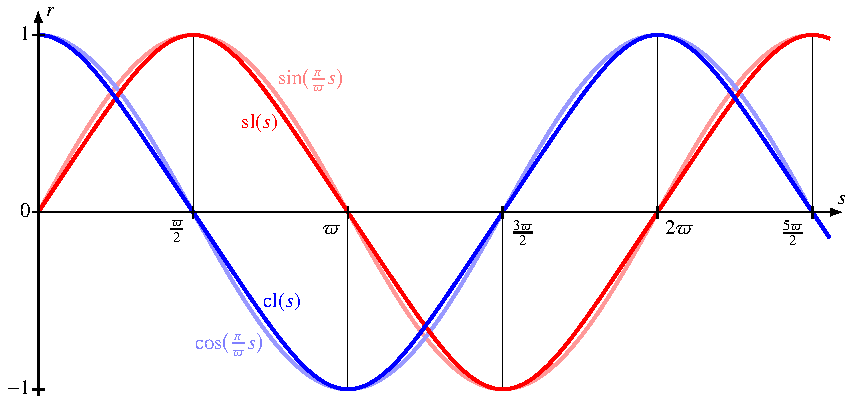
\includegraphics{chapters/110-elliptisch/images/slcl.pdf}
\caption{
Lemniskatischer Sinus und Kosinus sowie Sinus und Kosinus
mit derart skaliertem Argument, dass die Funktionen die gleichen Nullstellen
haben.
\label{buch:elliptisch:figure:slcl}}
\end{figure}


%\section*{Übungsaufgaben}
%\rhead{Übungsaufgaben}
%\aufgabetoplevel{chapters/020-exponential/uebungsaufgaben}
%\begin{uebungsaufgaben}
%\uebungsaufgabe{0}
%\uebungsaufgabe{1}
%\end{uebungsaufgaben}


%
% chapter.tex -- Beschreibung des Inhaltes
%
% (c) 2021 Prof Dr Andreas Müller, Hochschule Rapperswil
%
% !TeX spellcheck = de_CH
\chapter{Elliptische Funktionen
\label{buch:chapter:geometrie}}
\lhead{Elliptische Funktionen}
\rhead{}

Der Versuch, die Länge eines Ellipsenbogens zu berechnen, hat
in Abschnitt~\ref{buch:geometrie:subsection:hyperbeln-und-ellipsen}
zu Integralen geführt, die nicht in geschlossener Form ausgewertet
werden können.
Neben den dort gefundenen Integralen sind noch weitere, ähnlich
aufgebaute Integrale in dieser Familie zu finden.

%
% ellintegral.tex
%
% (c) 2021 Prof Dr Andreas Müller, OST Ostschweizer Fachhochschule
%
\section{Elliptische Integrale
\label{buch:elliptisch:section:integral}}
\rhead{Elliptisches Integral}
Bei der Berechnung des Ellipsenbogens in 
Abschnitt~\ref{buch:geometrie:subsection:hyperbeln-und-ellipsen}
sind wir auf ein Integral gestossen, welches sich nicht in geschlossener
Form ausdrücken liess.
Um solche Integrale in den Griff zu bekommen, ist es nötig, sie als
neue spezielle Funktionen zu definieren.

\subsection{Definition
\label{buch:elliptisch:subsection:definition}}
Ein {\em elliptisches Integral} ist ein Integral der Form
\index{elliptishes Integral}%
\index{Integral, elliptisch}%
\begin{equation}
\int R\left( x, \sqrt{p(x)}\right)\,dx
\label{buch:elliptisch:def:allgemein}
\end{equation}
wobei $R(x,y)$ eine rationale Funktion von zwei Variablen ist und
$p(x)$ ein Polynom dritten oder vierten Grades.
Hätte $p(x)$ ein mehrfache Nullstelle $x_0$, müsste es durch $(x-x_0)^2$
teilbar sein, man könnte also einen Faktor $(x-x_0)$ aus der
Wurzel im Integraneden von \eqref{buch:elliptisch:def:allgemein}
ausklammern und damit das Integral in eine Form bringen, wo $p(x)$
höchstens zweiten Grades ist.
Solche Integrale lassen sich meistens mit trigonometrischen Substitutionen
berechnen.
Wir verlangen daher, dass $p(x)$ keine mehrfachen Nullstellen hat.

Man kann zeigen, dass sich elliptische Integrale in Summen von
elementaren Funktionen und speziellen elliptischen Integralen 
der folgenden Form überführen lassen
\cite[Abschnitt 164, p.~506]{buch:smirnov32}.

\begin{definition}
\label{buch:elliptisch:def:integrale123}
Die elliptischen Integrale erster, zweiter und dritter Art sind die
Integrale
\[
\begin{aligned}
\text{1.~Art:}&&&
\int \frac{dx}{\sqrt{(1-x^2)(1-k^2x^2)}}
\\
\text{2.~Art:}&&&
\int \sqrt{\frac{1-k^2x^2}{1-x^2}}\,dx
\\
\text{3.~Art:}&&&
\int \frac{dx}{(1-nx^2)\sqrt{(1-x^2)(1-k^2x^2)}}
\end{aligned}
\]
mit $0<k<1$.
Es ist auch üblich, den Parameter $m=k^2$ zu verwenden.
\end{definition}

Wie gesagt lassen sich für diese unbestimmten Integrale keine 
geschlossenen Formen finden.
Es bleibt uns daher nichts anderes übrig, als die Integralgrenzen
festzulegen und damit eine Stammfunktion auszuwählen.

%
% Elliptisches Integral
%
\subsection{Vollständige elliptische Integrale
\label{buch:elliptisch:subsection:vollstaendig}}
In diesem Abschnitt legen wir beide Integrationsgrenzen fest und
untersuchen die entstehenenden Funktionen von den Parametern
$k$ und $n$.

\subsubsection{Definition der vollständigen elliptischen Integrale}
Da der Nenner in allen drei elliptischen Integralen eine Nullstelle
bei $\pm1$ hat, kann das Integral nur von $0$ bis $1$ erstreckt werden.

\begin{definition}
\label{buch:elliptisch:def:vollstintegrale123}
Die vollständigen elliptischen Integrale erster, zweiter und dritter
Art sind
\[
\begin{aligned}
\text{1.~Art:}&&
K(k)&=\int_0^1 \frac{dt}{\sqrt{(1-t^2)(1-k^2t^2)}} \\
\text{2.~Art:}&&
E(k)&=\int_0^1 \sqrt{\frac{1-k^2t^2}{1-t^2}}\,dt \\
\text{3.~Art:}&&
\Pi(n, k)&=\int_0^1\frac{dt}{(1-nt^2)\sqrt{(1-t^2)(1-k^2t^2)}} 
\end{aligned}
\]
mit $0<k<1$.
\end{definition}

Die Funktionen hängen stetig von $k$ ab.
Die Nullstellen des Faktors $1-k^2x^2$ liegen ausserhalb des
Integrationsintervalls und spielen daher keine Rolle.
Die Werte von $K(k)$ und $E(k)$ für $k=0$ können direkt berechnet
werden:
\begin{align*}
K(0)
=
E(0)
&=
\int_0^1 \frac{dt}{\sqrt{1-t^2}}=\frac{\pi}2.
\end{align*}
Das Integral $\Pi(n,0)$ ist etwas komplizierter.

Für $k\to 1$ ist $E(k)=1$, die Integrale $K(1)$ und $\Pi(n,1)$
sind dagegen divergent.

\subsubsection{Jacobi- und Legendre-Normalform}
Die Integrationsvariable $t$ der vollständigen elliptischen Integrale
kann durch die Substitution $t=\sin\varphi$ durch die Variable
$\varphi$ und das Integral über das Intervall $[0,1]$ durch ein
Integral über das Intervall $[0,\frac{\pi}2]$ ersetzt werden.
Mit
\[
\frac{dt}{d\varphi} = \cos\varphi = \sqrt{1-\sin^2\varphi}
\]
können die Funktionen $K(k)$, $E(k)$ und $\Pi(n,k)$ auch als
\begin{align*}
K(k)
&=
\int_0^{\frac{\pi}2}
\frac{
\sqrt{1-\sin^2\varphi}\,d\varphi
}{
\sqrt{(1-\sin^2\varphi)(1-k^2\sin^2\varphi)}
}
=
\int_0^{\frac{\pi}2}
\frac{d\varphi}{\sqrt{1-k^2\sin^2\varphi}}
\\
E(k)
&=
\int_0^{\frac{\pi}2}
\sqrt{\frac{1-k^2\sin^2\varphi}{1-\sin^2\varphi}}\sqrt{1-\sin^2\varphi}\,d\varphi
=
\int_0^{\frac{\pi}2}
\sqrt{1-k^2\sin^2\varphi}\,d\varphi
\\
\Pi(n,k)
&=
\int_0^{\frac{\pi}2}
\frac{
\sqrt{1-\sin^2\varphi}\,d\varphi
}{
(1-n\sin^2\varphi)\sqrt{(1-\sin^2\varphi)(1-k^2\sin^2\varphi)}
}
=
\int_0^{\frac{\pi}2}
\frac{
d\varphi
}{
(1-n\sin^2\varphi)\sqrt{1-k^2\sin^2\varphi}
}
\end{align*}
Diese Form wird auch die {\em Legendre-Normalform} der vollständigen 
\index{Legendre-Normalform}%
elliptischen Integrale genannt, während die Form von
Definition~\ref{buch:elliptisch:def:vollstintegrale123}
die {\em Jacobi-Normalform} heisst.
\index{Jacobi-Normalform}%

\subsubsection{Umfang einer Ellipse}
\begin{figure}
\centering
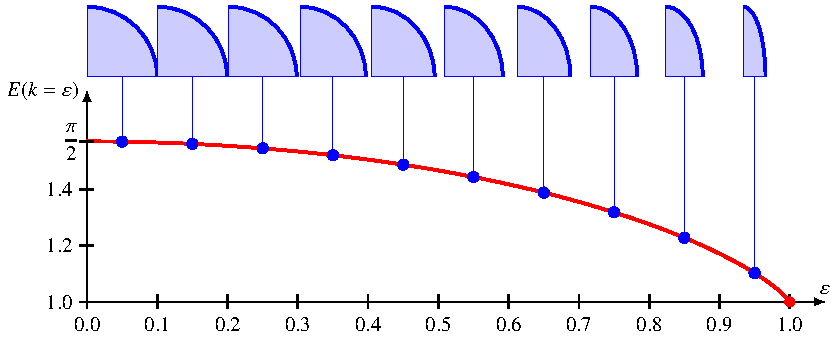
\includegraphics{chapters/110-elliptisch/images/ellipsenumfang.pdf}
\caption{Bogenlänge eines Viertels einer Ellipse mit Exzentrizität
$\varepsilon$.
\label{buch:elliptisch:fig:ellipsenumfang}}
\end{figure}
Wir zeigen, wie sich die Berechnung des Umfangs $U$ einer Ellipse
mit Halbachsen $a$ und $b$, $a\le b$, auf ein volltändiges elliptisches
Integral zurückführen lässt.
Der Fall $a>b$ kann behandelt werden, indem die $x$- und $y$-Koordinaten
vertauscht werden.

Die Parametrisierung
\[
t\mapsto \begin{pmatrix}a\cos t\\ b\sin t\end{pmatrix}
\]
einer Ellipse führt auf das Integral
\begin{align*}
U
&=
\int_0^{2\pi} \sqrt{a^2\sin^2t + b^2\cos^2 t}\,dt
\notag
\\
&=
4\int_0^{\frac{\pi}2}
\sqrt{a^2\sin^2t + b^2(1-\sin^2 t)}
\,dt
\notag
\\
&=
4b \int_0^{\frac{\pi}2} \sqrt{1-(b^2-a^2)/b^2\cdot \sin^2t}\,dt
\label{buch:elliptisch:eqn:umfangellipse}
\end{align*}
für den Umfang der Ellipse.
Bei einem Kreis ist $a=b$ und der zweite Term unter der Wurzel fällt weg,
der Umfang wird $4b\frac{\pi}2=2\pi b$.
Die Differenz $e^2=b^2-a^2$ ist die {\em lineare Exzentrizität} der Ellipse,
\index{lineare Exzentrizität}%
der Quotient $e/b$ wird die {\em numerische Exzentrizität} der Ellipse
genannt.
Insbesondere ist $k = \varepsilon$.

Das Integral~\eqref{buch:elliptisch:eqn:umfangellipse} erhält jetzt die
Form
\[
U
=
4b\int_0^{\frac{\pi}2} \sqrt{1-k^2\sin^2t}\,dt
\]
und ist damit als elliptisches Integral zweiter Art erkannt.
Für den Umfang der Ellipse finden wir damit die Formel
\[
U
=
4b E(k)
=
4b E(\varepsilon).
\]
Das vollständige elliptische Integral zweiter Art $E(\varepsilon)$
liefert also genau den Umfang der eines Viertels Ellipse mit
numerischer Exzentrizität $\varepsilon$ und kleiner Halbachse $1$.

\subsubsection{Komplementäre Integrale}
XXX Komplementäre Integrale \\

\subsubsection{Ableitung}
XXX Ableitung \\
XXX Stammfunktion \\

\subsection{Unvollständige elliptische Integrale}
XXX Vollständige und Unvollständige Integrale \\
XXX Additionstheoreme \\
XXX Parameterkonventionen \\

\subsection{Potenzreihe}
XXX Potenzreihen \\
XXX Als hypergeometrische Funktionen \\



\section{Jacobische elliptische Funktionen}

Für das elliptische Filter werden, wie es der Name bereits deutet, elliptische Funktionen gebraucht.
Wie die trigonometrischen Funktionen Zusammenhänge eines Kreises darlegen, beschreiben die elliptischen Funktionen Ellipsen.
Es ist daher naheliegend, dass der Kosinus des Tschebyscheff-Filters gegen ein elliptisches Pendant ausgetauscht werden könnte.
Der Begriff elliptische Funktion wird für sehr viele Funktionen gebraucht, daher ist es hier wichtig zu erwähnen, dass es ausschliesslich um die Jacobischen elliptischen Funktionen geht.

\subsection{Grundlegende Eigenschaften}

Die Jacobi elliptischen Funktionen werden ausführlich im Kapitel \ref{buch:elliptisch:section:jacobi} behandelt.
Im Wesentlichen erweitern die Jacobi elliptischen Funktionen die trigonometrische Funktionen für Ellipsen.
Zum Beispiel gibt es analog zum Sinus den elliptischen $\sn(z, k)$.
Im Gegensatz zum den trigonometrischen Funktionen haben die elliptischen Funktionen zwei Parameter.
Den \textit{elliptische Modul} $k$, der die Exzentrizität der Ellipse parametrisiert und das Winkelargument $z$.
Im Kreis ist der Radius für alle Winkel konstant, bei Ellipsen ändert sich das.
Dies hat zur Folge, dass bei einer Ellipse die Kreisbogenlänge nicht linear zum Winkel verläuft.
Darum kann hier nicht der gewohnte Winkel verwendet werden.
Das Winkelargument $z$ kann durch das elliptische Integral erster Art
\begin{equation}
    z
    =
    F(\phi, k)
    =
    \int_{0}^{\phi}
    \frac{
        d\theta
    }{
        \sqrt{
            1-k^2 \sin^2 \theta
        }
    }
\end{equation}
mit dem Winkel $\phi$ in Verbindung gebracht werden.

Dabei wird das vollständige und unvollständige elliptische integral unterschieden.
Beim vollständigen Integral
\begin{equation}
    K(k)
    =
    \int_{0}^{\pi / 2}
    \frac{
        d\theta
    }{
        \sqrt{
            1-k^2 \sin^2 \theta
        }
    }
\end{equation}
wird über ein viertel Ellipsenbogen integriert, also bis $\phi=\pi/2$ und liefert das Winkelargument für eine Vierteldrehung.
Die Zahl wird oft auch abgekürzt mit $K = K(k)$ und ist für das elliptische Filter sehr relevant.
Alle elliptischen Funktionen sind somit $4K$-periodisch.

Neben dem $\sn$ gibt es zwei weitere elliptische Basisfunktionen $\cn$ und $\dn$.
Dazu kommen noch weitere abgeleitete Funktionen, die durch Quotienten und Kehrwerte dieser Funktionen zustande kommen.
Insgesamt sind es die zwölf Funktionen
\begin{equation*}
    \sn \quad
    \ns \quad
    \scelliptic \quad
    \sd \quad
    \cn \quad
    \nc \quad
    \cs \quad
    \cd \quad
    \dn \quad
    \nd \quad
    \ds \quad
    \dc.
\end{equation*}

Die Jacobischen elliptischen Funktionen können mit der inversen Funktion des vollständigen elliptischen Integrals erster Art
\begin{equation}
    \phi = F^{-1}(z, k)
\end{equation}
definiert werden. Dabei ist zu beachten dass nur das $z$ Argument der Funktion invertiert wird, also
\begin{equation}
    z = F(\phi, k)
    \Leftrightarrow
    \phi = F^{-1}(z, k).
\end{equation}
Mithilfe von $F^{-1}$ kann zum Beispiel $sn^{-1}$ mit dem elliptischen Integral dargestellt werden:
\begin{equation}
    \sin(\phi)
    =
    \sin \left( F^{-1}(z, k) \right)
    =
    \sn(z, k)
    =
    w.
\end{equation}

% \begin{equation} %TODO remove unnecessary equations
%     \phi
%     =
%      F^{-1}(z, k)
%      =
%      \sin^{-1} \big( \sn (z, k ) \big)
%      =
%     \sin^{-1} ( w )
% \end{equation}

% \begin{equation}
%     F(\phi, k)
%     =
%     z
%     =
%     F( \sin^{-1} \big( \sn (z, k ) \big) , k)
%     =
%     F( \sin^{-1} ( w ), k)
% \end{equation}

% \begin{equation}
%     \sn^{-1}(w, k)
%     =
%     F(\phi, k),
%     \quad
%     \phi = \sin^{-1}(w)
% \end{equation}

\subsection{Die Funktion $\sn^{-1}$}

Beim Tschebyscheff-Filter konnten wir mit Betrachten des Arcuscosinus die Funktionalität erklären.
Für das Elliptische Filter machen wir die gleiche Betrachtung mit der $\sn^{-1}$-Funktion.
Der $\sn^{-1}$ ist durch das elliptische Integral
\begin{align}
    \sn^{-1}(w, k)
        & =
    \int_{0}^{\phi}
    \frac{
        d\theta
    }{
        \sqrt{
            1-k^2 \sin^2 \theta
        }
    },
    \quad
    \phi = \sin^{-1}(w)
    \\
        & =
    \int_{0}^{w}
    \frac{
        dt
    }{
        \sqrt{
            (1-t^2)(1-k^2 t^2)
        }
    }
\end{align}
beschrieben.
Dazu betrachten wir wieder den Integranden
\begin{equation}
    \frac{
        1
    }{
        \sqrt{
            (1-t^2)(1-k^2 t^2)
        }
    }.
\end{equation}
Beim $\cos^{-1}(x)$ haben wir gesehen, dass die analytische Fortsetzung bei $x < -1$ und $x > 1$ rechtwinklig in die komplexen Zahlen wandert.
Wenn man das Gleiche mit $\sn^{-1}(w, k)$ macht, erkennt man zwei interessante Stellen.
Die erste ist die gleiche wie beim $\cos^{-1}(x)$ nämlich bei $t = \pm 1$.
Der erste Term unter der Wurzel wird dann negativ, während der zweite noch positiv ist, da $k \leq 1$.
Ab diesem Punkt knickt die Funktion in die imaginäre Richtung ab.
Bei $t = 1/k$ ist auch der zweite Term negativ und die Funktion verläuft in die negative reelle Richtung.
Abbildung \ref{ellfilter:fig:sn} zeigt den Verlauf der Funktion in der komplexen Ebene.
\begin{figure}
    \centering
    \begin{tikzpicture}[>=stealth', auto, node distance=2cm, scale=1.2]

    \tikzstyle{zero} = [draw, circle, inner sep =0, minimum height=0.15cm]

    \tikzset{pole/.style={cross out, draw=black, minimum size=(0.15cm-\pgflinewidth), inner sep=0pt, outer sep=0pt}}

    \begin{scope}[xscale=0.9, yscale=1.8]

        \draw[gray, ->] (0,-1.5) -- (0,1.5) node[anchor=south]{$\mathrm{Im}~z$};
        \draw[gray, ->] (-5,0) -- (5,0) node[anchor=west]{$\mathrm{Re}~z$};

        \begin{scope}

            \clip(-4.5,-1.25) rectangle (4.5,1.25);

            \fill[yellow!30] (0,0) rectangle (1, 0.5);

            \begin{scope}[xshift=-1cm]

                \foreach \i in {-2,...,2} {
                    \foreach \j in {-2,...,1} {
                        \begin{scope}[xshift=\i*4cm, yshift=\j*1cm]
                            \draw[<-, blue!50] (0, 0) -- (0,0.5);
                            \draw[<-, cyan!50] (1, 0) -- (0,0);
                            \draw[<-, darkgreen!50] (2, 0) -- (1,0);
                            \draw[<-, orange!50] (2,0.5) -- (2, 0);
                            \draw[<-, red!50] (1, 0.5) -- (2,0.5);
                            \draw[<-, purple!50] (0, 0.5) -- (1,0.5);
                            \draw[<-, blue!50] (0,1) -- (0,0.5);
                            \draw[<-, orange!50] (2,0.5) -- (2, 1);
                            \draw[<-, red!50] (3, 0.5) -- (2,0.5);
                            \draw[<-, purple!50] (4, 0.5) -- (3,0.5);
                            \draw[<-, darkgreen!50] (2, 0) -- (3,0);
                            \draw[<-, cyan!50] (3, 0) -- (4,0);
                        \end{scope}
                    }
                }

                % \pause
                \draw[ultra thick, <-, darkgreen] (2, 0) -- (1,0);
                % \pause
                \draw[ultra thick, <-, orange] (2,0.5) -- (2, 0);
                % \pause
                \draw[ultra thick, <-, red] (1, 0.5) -- (2,0.5);
                % \pause
                \draw[ultra thick, <-, blue] (0, 0) -- (0,0.5);
                \draw[ultra thick, <-, purple] (0, 0.5) -- (1,0.5);
                \draw[ultra thick, <-, cyan] (1, 0) -- (0,0);
                % \pause


                \foreach \i in {-2,...,2} {
                    \foreach \j in {-2,...,1} {
                        \begin{scope}[xshift=\i*4cm, yshift=\j*1cm]
                            \node[zero] at ( 1, 0) {};
                            \node[zero] at ( 3, 0) {};
                            \node[pole] at ( 1,0.5) {};
                            \node[pole] at ( 3,0.5) {};
                        \end{scope}
                    }
                }

            \end{scope}

        \end{scope}

        \draw[gray] ( 1,0) +(0,0.1) -- +(0, -0.1) node[inner sep=0, anchor=north] {\small $K$};
        \draw[gray]  (0, 0.5) +(0.1, 0) -- +(-0.1, 0) node[inner sep=0, anchor=east]{\small $jK^\prime$};

    \end{scope}

    \node[zero] at (4,3) (n) {};
    \node[anchor=west] at (n.east) {Zero};
    \node[pole, below=0.25cm of n] (n) {};
    \node[anchor=west] at (n.east) {Pole};

    \begin{scope}[yshift=-4cm, xscale=0.75]

        \draw[gray, ->] (-6,0) -- (6,0) node[anchor=west]{$w$};

        \draw[ultra thick, ->, purple] (-5, 0) -- (-3, 0);
        \draw[ultra thick, ->, blue]      (-3, 0) -- (-2, 0);
        \draw[ultra thick, ->, cyan]       (-2, 0) -- (0, 0);
        \draw[ultra thick, ->, darkgreen]    (0, 0) -- (2, 0);
        \draw[ultra thick, ->, orange] (2, 0) -- (3, 0);
        \draw[ultra thick, ->, red] (3, 0) -- (5, 0);

        \node[anchor=south] at (-5,0) {$-\infty$};
        \node[anchor=south] at (-3,0) {$-1/k$};
        \node[anchor=south] at (-2,0) {$-1$};
        \node[anchor=south] at (0,0) {$0$};
        \node[anchor=south] at (2,0) {$1$};
        \node[anchor=south] at (3,0) {$1/k$};
        \node[anchor=south] at (5,0) {$\infty$};

    \end{scope}


\end{tikzpicture}
    \caption{
        $z$-Ebene der Funktion $z = \sn^{-1}(w, k)$.
        Die Funktion ist in der realen Achse $4K$-periodisch und in der imaginären Achse $2jK^\prime$-periodisch.
    }
    \label{ellfilter:fig:sn}
\end{figure}
In der reellen Richtung ist sie $4K(k)$-periodisch und in der imaginären Richtung $4K^\prime(k)$-periodisch, wobei $K^\prime$ das komplementäre vollständige Elliptische Integral ist:
\begin{equation}
    K^\prime(k)
    =
    \int_{0}^{\pi / 2}
    \frac{
        d\theta
    }{
        \sqrt{
            1-{k^\prime}^2 \sin^2 \theta
        }
    },
    \quad
    k^\prime = \sqrt{1-k^2}.
\end{equation}

%
% lemniskate.tex
%
% (c) 2021 Prof Dr Andreas Müller, OST Ostschweizer Fachhochschule
%
\section{Lemniskatischer Sinus
\label{buch:elliptisch:section:lemniskate}}
\rhead{Lemniskatischer Sinus}
Historisch war der {\em lemniskatische Sinus} die erste ellptische
Funktion, die Gauss bereits als 19-jähriger untersucht, aber nicht 
veröffentlich hat.
In diesem Abschnitt soll die Verbindung zu den Jacobischen
elliptischen Funktionen hergestellt werden.

\subsection{Lemniskate
\label{buch:gemotrie:subsection:lemniskate}}
\begin{figure}
\centering
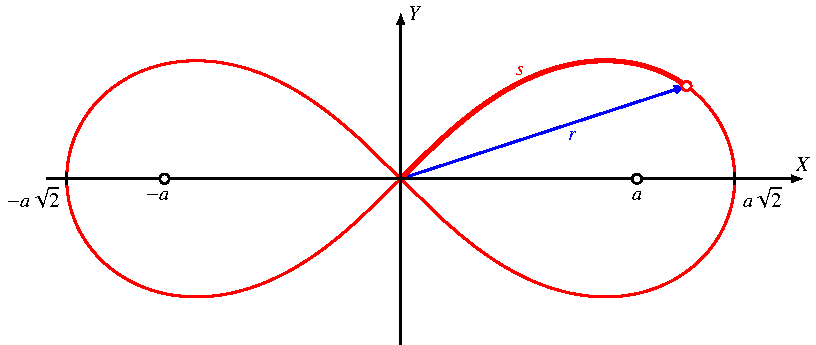
\includegraphics{chapters/110-elliptisch/images/lemniskate.pdf}
\caption{Bogenlänge und Radius der Lemniskate von Bernoulli.
\label{buch:elliptisch:fig:lemniskate}}
\end{figure}
Die Lemniskate von Bernoulli ist die Kurve vierten Grades mit der Gleichung
\begin{equation}
(X^2+Y^2)^2 = 2a^2(X^2-Y^2).
\label{buch:elliptisch:eqn:lemniskate}
\end{equation}
Sie ist in Abbildung~\ref{buch:elliptisch:fig:lemniskate}
dargestellt.
Die beiden Scheitel der Lemniskate befinden sich bei $X_s=\pm a\sqrt{2}$.
Dividiert man die Gleichung der Lemniskate durch $X_s^2=4a^4$ entsteht 
\begin{equation}
\biggl(
\biggl(\frac{X}{a\sqrt{2}}\biggr)^2
+
\biggl(\frac{Y}{a\sqrt{2}}\biggr)^2
\biggr)^2
=
2\frac{a^2}{2a^2}\biggl(
\biggl(\frac{X}{a\sqrt{2}}\biggr)^2
-
\biggl(\frac{Y}{a\sqrt{2}}\biggr)^2
\biggr).
\qquad
\Leftrightarrow
\qquad
(x^2+y^2)^2 = x^2-y^2,
\label{buch:elliptisch:eqn:lemniskatenormiert}
\end{equation}
wobei wir $x=X/a\sqrt{2}$ und $y=Y/a\sqrt{2}$ gesetzt haben.
In dieser Normierung liegen die Scheitel bei $\pm 1$.
Dies ist die Skalierung, die für die Definition des lemniskatischen
Sinus und Kosinus verwendet werden soll.

In Polarkoordinaten $x=r\cos\varphi$ und $y=r\sin\varphi$
gilt nach Einsetzen in \eqref{buch:elliptisch:eqn:lemniskatenormiert}
\begin{equation}
r^4
=
r^2(\cos^2\varphi-\sin^2\varphi)
=
r^2\cos2\varphi
\qquad\Rightarrow\qquad
r^2 = \cos 2\varphi
\label{buch:elliptisch:eqn:lemniskatepolar}
\end{equation}
als Darstellung der Lemniskate in Polardarstellung.
Sie gilt für Winkel $\varphi\in[-\frac{\pi}4,\frac{\pi}4]$ für das
rechte Blatt und $\varphi\in[\frac{3\pi}4,\frac{5\pi}4]$ für das linke
Blatt der Lemniskate.

\subsection{Bogenlänge}
Die Funktionen
\begin{equation}
x(r) = \frac{r}{\sqrt{2}}\sqrt{1+r^2},
\quad
y(r) = \frac{r}{\sqrt{2}}\sqrt{1-r^2}
\label{buch:geometrie:eqn:lemniskateparam}
\end{equation}
erfüllen
\begin{align*}
x(r)^2-y(r)^2
&=
\frac{r^2(1+r^2)}{2}-\frac{r^2(1-r^2)}{2}
\\
&
=
r^4
=
(x(r)^2 + y(r)^2)^2,
\end{align*}
sie stellen also eine Parametrisierung der Lemniskate dar.

Mit Hilfe der Parametrisierung~\eqref{buch:geometrie:eqn:lemniskateparam}
kann man die Länge $s$ des in Abbildung~\ref{buch:elliptisch:fig:lemniskate}
dargestellten Bogens der Lemniskate berechnen.
Dazu benötigt man die Ableitungen nach $r$, die man mit der Produkt- und
Kettenregel berechnen kann:
\begin{align*}
\dot{x}(r)
&=
\frac{\sqrt{1+r^2}}{\sqrt{2}}
+
\frac{r^2}{\sqrt{2}\sqrt{1+r^2}}
&&\Rightarrow&
\dot{x}(r)^2
&=
\frac{1+r^2}{2} +r^2 + \frac{r^4}{2(1+r^2)}
\\
\dot{y}(r)
&=
\frac{\sqrt{1-r^2}}{\sqrt{2}}
-
\frac{r^2}{\sqrt{2}\sqrt{1-r^2}}
&&\Rightarrow&
\dot{y}(r)^2
&=
\frac{1-r^2}{2} -r^2 + \frac{r^4}{2(1-r^2)}
\end{align*}
Die Summe der Quadrate ist
\begin{align*}
\dot{x}(r)^2 + \dot{y}(r)^2
&=
1 + r^4\frac{1-r^2+1+r^2}{2(1+r^2)(1-r^2)}
=
1+r^4\frac{2}{2(1-r^4)}
=
\frac{1-r^4+r^4}{1-r^4}
=
\frac1{1-r^4}.
\end{align*}
Durch Einsetzen in das Integral für die Bogenlänge bekommt man
\begin{equation}
s(r)
=
\int_0^r
\frac{1}{\sqrt{1-t^4}}\,dt.
\label{buch:elliptisch:eqn:lemniskatebogenlaenge}
\end{equation}

%
% Als elliptisches Integral
%
\subsection{Darstellung als elliptisches Integral}
Das unvollständige elliptische Integral erster Art mit Parameter
$k^2=-1$ oder $k=i$ ist
\[
K(r,i)
=
\int_0^x \frac{dt}{\sqrt{(1-t^2)(1-i^2 t^2)}}
=
\int_0^x \frac{dt}{\sqrt{(1-t^2)(1-(-1)t^2)}}
=
\int_0^x \frac{dt}{\sqrt{1-t^4}}
=
s(r).
\]
Der lemniskatische Sinus ist also eine Umkehrfunktion des
elliptischen Integrals erster Art für den speziellen Wert $i$ des
Parameters $k$.

Die Länge des rechten Blattes der Lemniskate wird mit $\varpi$ bezeichnet
und hat den numerischen Wert
\[
\varpi
=
2\int_0^1\sqrt{\frac{1}{1-t^4}}\,dt
=
2.6220575542.
\]
$\varpi$ ist auch als die {\em lemniskatische Konstante} bekannt.
\index{lemniskatische Konstante}%
Der Lemniskatenbogen zwischen dem Nullpunkt und $(1,0)$ hat die Länge
$\varpi/2$.

%
%  Bogenlängenparametrisierung
%
\subsection{Bogenlängenparametrisierung}
Die Lemniskate mit der Gleichung
\[
(X^2+X^2)^2=2(X^2-X^2)
\]
(der Fall $a=1$ in \eqref{buch:elliptisch:eqn:lemniskate})
kann mit Jacobischen elliptischen Funktionen
parametrisiert werden.
Dazu schreibt man
\[
\left.
\begin{aligned}
X(t)
&=
\sqrt{2}\operatorname{cn}(t,k) \operatorname{dn}(t,k)
\\
Y(t)
&=
\phantom{\sqrt{2}}
\operatorname{cn}(t,k) \operatorname{sn}(t,k)
\end{aligned}
\quad\right\}
\qquad\text{mit $k=\displaystyle\frac{1}{\sqrt{2}}$}
\]
und berechnet die beiden Seiten der definierenden Gleichung der
Lemniskate.
Zunächst ist
\begin{align*}
X(t)^2
&=
2\operatorname{cn}(t,k)^2
\operatorname{dn}(t,k)^2
\\
Y(t)^2
&=
\operatorname{cn}(t,k)^2
\operatorname{sn}(t,k)^2
\\
X(t)^2+Y(t)^2
&=
2\operatorname{cn}(t,k)^2
\bigl(
\underbrace{
\operatorname{dn}(t,k)^2
+{\textstyle\frac12}
\operatorname{sn}(t,k)^2
}_{\displaystyle =1}
\bigr)
%\\
%&
=
2\operatorname{cn}(t,k)^2
\\
X(t)^2-Y(t)^2
&=
\operatorname{cn}(t,k)^2
\bigl(
2\operatorname{dn}(t,k)^2 - \operatorname{sn}(t,k)^2
\bigr)
\\
&=
\operatorname{cn}(t,k)^2
\bigl(
2\bigl({\textstyle\frac12}+{\textstyle\frac12}\operatorname{cn}(t,k)^2\bigr)
-
\bigl(1-\operatorname{cn}(t,k)^2\bigr)
\bigr)
\\
&=
2\operatorname{cn}(t,k)^4
\\
\Rightarrow\qquad
(X(t)^2+Y(t)^2)^2
&=
4\operatorname{cn}(t,k)^4
=
2(X(t)^2-Y(t)^2).
\end{align*}
Wir zeigen jetzt, dass dies tatsächlich eine Bogenlängenparametrisierung
der Lemniskate ist.
Dazu berechnen wir die Ableitungen
\begin{align*}
\dot{X}(t)
&=
\sqrt{2}\operatorname{cn}'(t,k)\operatorname{dn}(t,k)
+
\sqrt{2}\operatorname{cn}(t,k)\operatorname{dn}'(t,k)
\\
&=
-\sqrt{2}\operatorname{sn}(t,k)\operatorname{dn}(t,k)^2
-\frac12\sqrt{2}\operatorname{sn}(t,k)\operatorname{cn}(t,k)^2
\\
&=
-\sqrt{2}\operatorname{sn}(t,k)\bigl(
1-{\textstyle\frac12}\operatorname{sn}(t,k)^2
+{\textstyle\frac12}-{\textstyle\frac12}\operatorname{sn}(u,t)^2
\bigr)
\\
&=
\sqrt{2}\operatorname{sn}(t,k)
\bigl(
{\textstyle \frac32}-\operatorname{sn}(t,k)^2
\bigr)
\\
\dot{X}(t)^2
&=
2\operatorname{sn}(t,k)^2
\bigl(
{\textstyle \frac32}-\operatorname{sn}(t,k)^2
\bigr)^2
\\
&=
{\textstyle\frac{9}{2}}\operatorname{sn}(t,k)^2
-
6\operatorname{sn}(t,k)^4
+2\operatorname{sn}(t,k)^6
\\
\dot{Y}(t)
&=
\operatorname{cn}'(t,k)\operatorname{sn}(t,k)
+
\operatorname{cn}(t,k)\operatorname{sn}'(t,k)
\\
&=
-\operatorname{sn}(t,k)^2
\operatorname{dn}(t,k)
+\operatorname{cn}(t,k)^2
\operatorname{dn}(t,k)
\\
&=
\operatorname{dn}(t,k)\bigl(1-2\operatorname{sn}(t,k)^2\bigr)
\\
\dot{Y}(t)^2
&=
\bigl(1-{\textstyle\frac12}\operatorname{sn}(t,k)^2\bigr)
\bigl(1-2\operatorname|{sn}(t,k)^2\bigr)^2
\\
&=
1-{\textstyle\frac{9}{2}}\operatorname{sn}(t,k)^2
+6\operatorname{sn}(t,k)^4
-2\operatorname{sn}(t,k)^6
\\
\dot{X}(t)^2 + \dot{Y}(t)^2
&=
1.
\end{align*}
Dies bedeutet, dass die Bogenlänge zwischen den Parameterwerten $0$ und $s$
\[
\int_0^s
\sqrt{\dot{X}(t)^2 + \dot{Y}(t)^2}
\,dt
=
\int_0^s\,dt
=
s,
\]
der Parameter $t$ ist also ein Bogenlängenparameter.

Die mit dem Faktor $1/\sqrt{2}$ skalierte Standard-Lemniskate mit der
Gleichung
\[
(x^2+y^2)^2 = x^2-y^2
\]
hat daher eine Bogenlängenparametrisierung mit
\begin{equation}
\begin{aligned}
x(t)
&=
\phantom{\frac{1}{\sqrt{2}}}
\operatorname{cn}(\sqrt{2}t,k)\operatorname{dn}(\sqrt{2}t,k)
\\
y(t)
&=
\frac{1}{\sqrt{2}}\operatorname{cn}(\sqrt{2}t,k)\operatorname{sn}(\sqrt{2}t,k)
\end{aligned}
\label{buch:elliptisch:lemniskate:bogenlaenge}
\end{equation}

\subsection{Der lemniskatische Sinus und Kosinus}
Der Sinus Berechnet die Gegenkathete zu einer gegebenen Bogenlänge des
Kreises, er ist die Umkehrfunktion der Funktion, die der Gegenkathete
die Bogenlänge zuordnet.

Daher ist es naheliegend, die Umkehrfunktion von $s(r)$ in 
\eqref{buch:elliptisch:eqn:lemniskatebogenlaenge}
den {\em lemniskatischen Sinus} zu nennen mit der Bezeichnung
$r=\operatorname{sl} s$.

Der Kosinus ist der Sinus des komplementären Winkels.
Auch für die lemniskatische Bogenlänge $s(r)$ lässt sich eine
komplementäre Bogenlänge definieren, nämlich die Bogenlänge zwischen
dem Punkt $(x(r), y(r))$ und $(1,0)$.

Da die Parametrisierung~\eqref{buch:elliptisch:lemniskate:bogenlaenge}
eine Bogenlängenparametrisierung ist, darf man $t=s$ schreiben.
Dann kann man aber auch $r(s)$ daraus berechnen,
es ist
\[
r(s)^2
=
x(s)^2 + y(s)^2
=
\operatorname{cn}(s\sqrt{2},k)^2
\qquad\Rightarrow\qquad
r(s)
=
\operatorname{cn}(s\sqrt{2},k)
\]

\begin{figure}
\centering
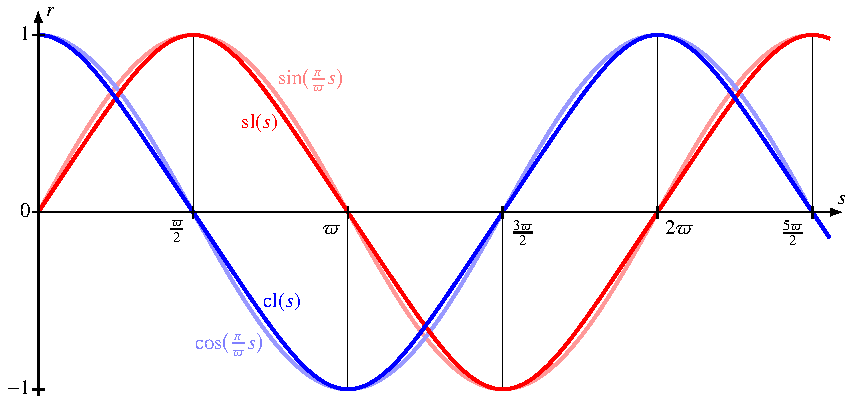
\includegraphics{chapters/110-elliptisch/images/slcl.pdf}
\caption{
Lemniskatischer Sinus und Kosinus sowie Sinus und Kosinus
mit derart skaliertem Argument, dass die Funktionen die gleichen Nullstellen
haben.
\label{buch:elliptisch:figure:slcl}}
\end{figure}


%\section*{Übungsaufgaben}
%\rhead{Übungsaufgaben}
%\aufgabetoplevel{chapters/020-exponential/uebungsaufgaben}
%\begin{uebungsaufgaben}
%\uebungsaufgabe{0}
%\uebungsaufgabe{1}
%\end{uebungsaufgaben}



% analytisch definierte spezielle Funktionen
%
% chapter.tex -- Beschreibung des Inhaltes
%
% (c) 2021 Prof Dr Andreas Müller, Hochschule Rapperswil
%
% !TeX spellcheck = de_CH
\chapter{Elliptische Funktionen
\label{buch:chapter:geometrie}}
\lhead{Elliptische Funktionen}
\rhead{}

Der Versuch, die Länge eines Ellipsenbogens zu berechnen, hat
in Abschnitt~\ref{buch:geometrie:subsection:hyperbeln-und-ellipsen}
zu Integralen geführt, die nicht in geschlossener Form ausgewertet
werden können.
Neben den dort gefundenen Integralen sind noch weitere, ähnlich
aufgebaute Integrale in dieser Familie zu finden.

%
% ellintegral.tex
%
% (c) 2021 Prof Dr Andreas Müller, OST Ostschweizer Fachhochschule
%
\section{Elliptische Integrale
\label{buch:elliptisch:section:integral}}
\rhead{Elliptisches Integral}
Bei der Berechnung des Ellipsenbogens in 
Abschnitt~\ref{buch:geometrie:subsection:hyperbeln-und-ellipsen}
sind wir auf ein Integral gestossen, welches sich nicht in geschlossener
Form ausdrücken liess.
Um solche Integrale in den Griff zu bekommen, ist es nötig, sie als
neue spezielle Funktionen zu definieren.

\subsection{Definition
\label{buch:elliptisch:subsection:definition}}
Ein {\em elliptisches Integral} ist ein Integral der Form
\index{elliptishes Integral}%
\index{Integral, elliptisch}%
\begin{equation}
\int R\left( x, \sqrt{p(x)}\right)\,dx
\label{buch:elliptisch:def:allgemein}
\end{equation}
wobei $R(x,y)$ eine rationale Funktion von zwei Variablen ist und
$p(x)$ ein Polynom dritten oder vierten Grades.
Hätte $p(x)$ ein mehrfache Nullstelle $x_0$, müsste es durch $(x-x_0)^2$
teilbar sein, man könnte also einen Faktor $(x-x_0)$ aus der
Wurzel im Integraneden von \eqref{buch:elliptisch:def:allgemein}
ausklammern und damit das Integral in eine Form bringen, wo $p(x)$
höchstens zweiten Grades ist.
Solche Integrale lassen sich meistens mit trigonometrischen Substitutionen
berechnen.
Wir verlangen daher, dass $p(x)$ keine mehrfachen Nullstellen hat.

Man kann zeigen, dass sich elliptische Integrale in Summen von
elementaren Funktionen und speziellen elliptischen Integralen 
der folgenden Form überführen lassen
\cite[Abschnitt 164, p.~506]{buch:smirnov32}.

\begin{definition}
\label{buch:elliptisch:def:integrale123}
Die elliptischen Integrale erster, zweiter und dritter Art sind die
Integrale
\[
\begin{aligned}
\text{1.~Art:}&&&
\int \frac{dx}{\sqrt{(1-x^2)(1-k^2x^2)}}
\\
\text{2.~Art:}&&&
\int \sqrt{\frac{1-k^2x^2}{1-x^2}}\,dx
\\
\text{3.~Art:}&&&
\int \frac{dx}{(1-nx^2)\sqrt{(1-x^2)(1-k^2x^2)}}
\end{aligned}
\]
mit $0<k<1$.
Es ist auch üblich, den Parameter $m=k^2$ zu verwenden.
\end{definition}

Wie gesagt lassen sich für diese unbestimmten Integrale keine 
geschlossenen Formen finden.
Es bleibt uns daher nichts anderes übrig, als die Integralgrenzen
festzulegen und damit eine Stammfunktion auszuwählen.

%
% Elliptisches Integral
%
\subsection{Vollständige elliptische Integrale
\label{buch:elliptisch:subsection:vollstaendig}}
In diesem Abschnitt legen wir beide Integrationsgrenzen fest und
untersuchen die entstehenenden Funktionen von den Parametern
$k$ und $n$.

\subsubsection{Definition der vollständigen elliptischen Integrale}
Da der Nenner in allen drei elliptischen Integralen eine Nullstelle
bei $\pm1$ hat, kann das Integral nur von $0$ bis $1$ erstreckt werden.

\begin{definition}
\label{buch:elliptisch:def:vollstintegrale123}
Die vollständigen elliptischen Integrale erster, zweiter und dritter
Art sind
\[
\begin{aligned}
\text{1.~Art:}&&
K(k)&=\int_0^1 \frac{dt}{\sqrt{(1-t^2)(1-k^2t^2)}} \\
\text{2.~Art:}&&
E(k)&=\int_0^1 \sqrt{\frac{1-k^2t^2}{1-t^2}}\,dt \\
\text{3.~Art:}&&
\Pi(n, k)&=\int_0^1\frac{dt}{(1-nt^2)\sqrt{(1-t^2)(1-k^2t^2)}} 
\end{aligned}
\]
mit $0<k<1$.
\end{definition}

Die Funktionen hängen stetig von $k$ ab.
Die Nullstellen des Faktors $1-k^2x^2$ liegen ausserhalb des
Integrationsintervalls und spielen daher keine Rolle.
Die Werte von $K(k)$ und $E(k)$ für $k=0$ können direkt berechnet
werden:
\begin{align*}
K(0)
=
E(0)
&=
\int_0^1 \frac{dt}{\sqrt{1-t^2}}=\frac{\pi}2.
\end{align*}
Das Integral $\Pi(n,0)$ ist etwas komplizierter.

Für $k\to 1$ ist $E(k)=1$, die Integrale $K(1)$ und $\Pi(n,1)$
sind dagegen divergent.

\subsubsection{Jacobi- und Legendre-Normalform}
Die Integrationsvariable $t$ der vollständigen elliptischen Integrale
kann durch die Substitution $t=\sin\varphi$ durch die Variable
$\varphi$ und das Integral über das Intervall $[0,1]$ durch ein
Integral über das Intervall $[0,\frac{\pi}2]$ ersetzt werden.
Mit
\[
\frac{dt}{d\varphi} = \cos\varphi = \sqrt{1-\sin^2\varphi}
\]
können die Funktionen $K(k)$, $E(k)$ und $\Pi(n,k)$ auch als
\begin{align*}
K(k)
&=
\int_0^{\frac{\pi}2}
\frac{
\sqrt{1-\sin^2\varphi}\,d\varphi
}{
\sqrt{(1-\sin^2\varphi)(1-k^2\sin^2\varphi)}
}
=
\int_0^{\frac{\pi}2}
\frac{d\varphi}{\sqrt{1-k^2\sin^2\varphi}}
\\
E(k)
&=
\int_0^{\frac{\pi}2}
\sqrt{\frac{1-k^2\sin^2\varphi}{1-\sin^2\varphi}}\sqrt{1-\sin^2\varphi}\,d\varphi
=
\int_0^{\frac{\pi}2}
\sqrt{1-k^2\sin^2\varphi}\,d\varphi
\\
\Pi(n,k)
&=
\int_0^{\frac{\pi}2}
\frac{
\sqrt{1-\sin^2\varphi}\,d\varphi
}{
(1-n\sin^2\varphi)\sqrt{(1-\sin^2\varphi)(1-k^2\sin^2\varphi)}
}
=
\int_0^{\frac{\pi}2}
\frac{
d\varphi
}{
(1-n\sin^2\varphi)\sqrt{1-k^2\sin^2\varphi}
}
\end{align*}
Diese Form wird auch die {\em Legendre-Normalform} der vollständigen 
\index{Legendre-Normalform}%
elliptischen Integrale genannt, während die Form von
Definition~\ref{buch:elliptisch:def:vollstintegrale123}
die {\em Jacobi-Normalform} heisst.
\index{Jacobi-Normalform}%

\subsubsection{Umfang einer Ellipse}
\begin{figure}
\centering
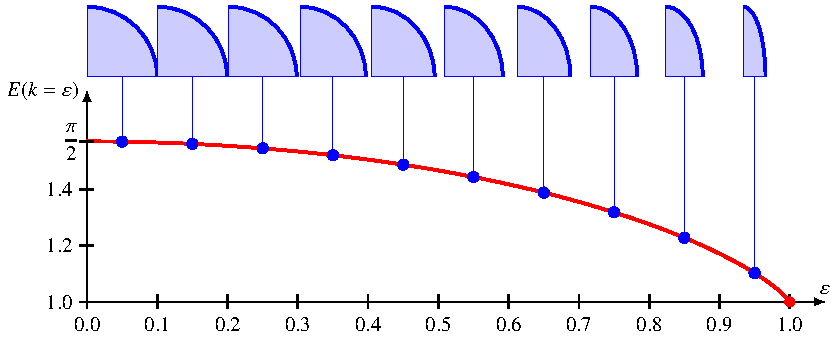
\includegraphics{chapters/110-elliptisch/images/ellipsenumfang.pdf}
\caption{Bogenlänge eines Viertels einer Ellipse mit Exzentrizität
$\varepsilon$.
\label{buch:elliptisch:fig:ellipsenumfang}}
\end{figure}
Wir zeigen, wie sich die Berechnung des Umfangs $U$ einer Ellipse
mit Halbachsen $a$ und $b$, $a\le b$, auf ein volltändiges elliptisches
Integral zurückführen lässt.
Der Fall $a>b$ kann behandelt werden, indem die $x$- und $y$-Koordinaten
vertauscht werden.

Die Parametrisierung
\[
t\mapsto \begin{pmatrix}a\cos t\\ b\sin t\end{pmatrix}
\]
einer Ellipse führt auf das Integral
\begin{align*}
U
&=
\int_0^{2\pi} \sqrt{a^2\sin^2t + b^2\cos^2 t}\,dt
\notag
\\
&=
4\int_0^{\frac{\pi}2}
\sqrt{a^2\sin^2t + b^2(1-\sin^2 t)}
\,dt
\notag
\\
&=
4b \int_0^{\frac{\pi}2} \sqrt{1-(b^2-a^2)/b^2\cdot \sin^2t}\,dt
\label{buch:elliptisch:eqn:umfangellipse}
\end{align*}
für den Umfang der Ellipse.
Bei einem Kreis ist $a=b$ und der zweite Term unter der Wurzel fällt weg,
der Umfang wird $4b\frac{\pi}2=2\pi b$.
Die Differenz $e^2=b^2-a^2$ ist die {\em lineare Exzentrizität} der Ellipse,
\index{lineare Exzentrizität}%
der Quotient $e/b$ wird die {\em numerische Exzentrizität} der Ellipse
genannt.
Insbesondere ist $k = \varepsilon$.

Das Integral~\eqref{buch:elliptisch:eqn:umfangellipse} erhält jetzt die
Form
\[
U
=
4b\int_0^{\frac{\pi}2} \sqrt{1-k^2\sin^2t}\,dt
\]
und ist damit als elliptisches Integral zweiter Art erkannt.
Für den Umfang der Ellipse finden wir damit die Formel
\[
U
=
4b E(k)
=
4b E(\varepsilon).
\]
Das vollständige elliptische Integral zweiter Art $E(\varepsilon)$
liefert also genau den Umfang der eines Viertels Ellipse mit
numerischer Exzentrizität $\varepsilon$ und kleiner Halbachse $1$.

\subsubsection{Komplementäre Integrale}
XXX Komplementäre Integrale \\

\subsubsection{Ableitung}
XXX Ableitung \\
XXX Stammfunktion \\

\subsection{Unvollständige elliptische Integrale}
XXX Vollständige und Unvollständige Integrale \\
XXX Additionstheoreme \\
XXX Parameterkonventionen \\

\subsection{Potenzreihe}
XXX Potenzreihen \\
XXX Als hypergeometrische Funktionen \\



\section{Jacobische elliptische Funktionen}

Für das elliptische Filter werden, wie es der Name bereits deutet, elliptische Funktionen gebraucht.
Wie die trigonometrischen Funktionen Zusammenhänge eines Kreises darlegen, beschreiben die elliptischen Funktionen Ellipsen.
Es ist daher naheliegend, dass der Kosinus des Tschebyscheff-Filters gegen ein elliptisches Pendant ausgetauscht werden könnte.
Der Begriff elliptische Funktion wird für sehr viele Funktionen gebraucht, daher ist es hier wichtig zu erwähnen, dass es ausschliesslich um die Jacobischen elliptischen Funktionen geht.

\subsection{Grundlegende Eigenschaften}

Die Jacobi elliptischen Funktionen werden ausführlich im Kapitel \ref{buch:elliptisch:section:jacobi} behandelt.
Im Wesentlichen erweitern die Jacobi elliptischen Funktionen die trigonometrische Funktionen für Ellipsen.
Zum Beispiel gibt es analog zum Sinus den elliptischen $\sn(z, k)$.
Im Gegensatz zum den trigonometrischen Funktionen haben die elliptischen Funktionen zwei Parameter.
Den \textit{elliptische Modul} $k$, der die Exzentrizität der Ellipse parametrisiert und das Winkelargument $z$.
Im Kreis ist der Radius für alle Winkel konstant, bei Ellipsen ändert sich das.
Dies hat zur Folge, dass bei einer Ellipse die Kreisbogenlänge nicht linear zum Winkel verläuft.
Darum kann hier nicht der gewohnte Winkel verwendet werden.
Das Winkelargument $z$ kann durch das elliptische Integral erster Art
\begin{equation}
    z
    =
    F(\phi, k)
    =
    \int_{0}^{\phi}
    \frac{
        d\theta
    }{
        \sqrt{
            1-k^2 \sin^2 \theta
        }
    }
\end{equation}
mit dem Winkel $\phi$ in Verbindung gebracht werden.

Dabei wird das vollständige und unvollständige elliptische integral unterschieden.
Beim vollständigen Integral
\begin{equation}
    K(k)
    =
    \int_{0}^{\pi / 2}
    \frac{
        d\theta
    }{
        \sqrt{
            1-k^2 \sin^2 \theta
        }
    }
\end{equation}
wird über ein viertel Ellipsenbogen integriert, also bis $\phi=\pi/2$ und liefert das Winkelargument für eine Vierteldrehung.
Die Zahl wird oft auch abgekürzt mit $K = K(k)$ und ist für das elliptische Filter sehr relevant.
Alle elliptischen Funktionen sind somit $4K$-periodisch.

Neben dem $\sn$ gibt es zwei weitere elliptische Basisfunktionen $\cn$ und $\dn$.
Dazu kommen noch weitere abgeleitete Funktionen, die durch Quotienten und Kehrwerte dieser Funktionen zustande kommen.
Insgesamt sind es die zwölf Funktionen
\begin{equation*}
    \sn \quad
    \ns \quad
    \scelliptic \quad
    \sd \quad
    \cn \quad
    \nc \quad
    \cs \quad
    \cd \quad
    \dn \quad
    \nd \quad
    \ds \quad
    \dc.
\end{equation*}

Die Jacobischen elliptischen Funktionen können mit der inversen Funktion des vollständigen elliptischen Integrals erster Art
\begin{equation}
    \phi = F^{-1}(z, k)
\end{equation}
definiert werden. Dabei ist zu beachten dass nur das $z$ Argument der Funktion invertiert wird, also
\begin{equation}
    z = F(\phi, k)
    \Leftrightarrow
    \phi = F^{-1}(z, k).
\end{equation}
Mithilfe von $F^{-1}$ kann zum Beispiel $sn^{-1}$ mit dem elliptischen Integral dargestellt werden:
\begin{equation}
    \sin(\phi)
    =
    \sin \left( F^{-1}(z, k) \right)
    =
    \sn(z, k)
    =
    w.
\end{equation}

% \begin{equation} %TODO remove unnecessary equations
%     \phi
%     =
%      F^{-1}(z, k)
%      =
%      \sin^{-1} \big( \sn (z, k ) \big)
%      =
%     \sin^{-1} ( w )
% \end{equation}

% \begin{equation}
%     F(\phi, k)
%     =
%     z
%     =
%     F( \sin^{-1} \big( \sn (z, k ) \big) , k)
%     =
%     F( \sin^{-1} ( w ), k)
% \end{equation}

% \begin{equation}
%     \sn^{-1}(w, k)
%     =
%     F(\phi, k),
%     \quad
%     \phi = \sin^{-1}(w)
% \end{equation}

\subsection{Die Funktion $\sn^{-1}$}

Beim Tschebyscheff-Filter konnten wir mit Betrachten des Arcuscosinus die Funktionalität erklären.
Für das Elliptische Filter machen wir die gleiche Betrachtung mit der $\sn^{-1}$-Funktion.
Der $\sn^{-1}$ ist durch das elliptische Integral
\begin{align}
    \sn^{-1}(w, k)
        & =
    \int_{0}^{\phi}
    \frac{
        d\theta
    }{
        \sqrt{
            1-k^2 \sin^2 \theta
        }
    },
    \quad
    \phi = \sin^{-1}(w)
    \\
        & =
    \int_{0}^{w}
    \frac{
        dt
    }{
        \sqrt{
            (1-t^2)(1-k^2 t^2)
        }
    }
\end{align}
beschrieben.
Dazu betrachten wir wieder den Integranden
\begin{equation}
    \frac{
        1
    }{
        \sqrt{
            (1-t^2)(1-k^2 t^2)
        }
    }.
\end{equation}
Beim $\cos^{-1}(x)$ haben wir gesehen, dass die analytische Fortsetzung bei $x < -1$ und $x > 1$ rechtwinklig in die komplexen Zahlen wandert.
Wenn man das Gleiche mit $\sn^{-1}(w, k)$ macht, erkennt man zwei interessante Stellen.
Die erste ist die gleiche wie beim $\cos^{-1}(x)$ nämlich bei $t = \pm 1$.
Der erste Term unter der Wurzel wird dann negativ, während der zweite noch positiv ist, da $k \leq 1$.
Ab diesem Punkt knickt die Funktion in die imaginäre Richtung ab.
Bei $t = 1/k$ ist auch der zweite Term negativ und die Funktion verläuft in die negative reelle Richtung.
Abbildung \ref{ellfilter:fig:sn} zeigt den Verlauf der Funktion in der komplexen Ebene.
\begin{figure}
    \centering
    \begin{tikzpicture}[>=stealth', auto, node distance=2cm, scale=1.2]

    \tikzstyle{zero} = [draw, circle, inner sep =0, minimum height=0.15cm]

    \tikzset{pole/.style={cross out, draw=black, minimum size=(0.15cm-\pgflinewidth), inner sep=0pt, outer sep=0pt}}

    \begin{scope}[xscale=0.9, yscale=1.8]

        \draw[gray, ->] (0,-1.5) -- (0,1.5) node[anchor=south]{$\mathrm{Im}~z$};
        \draw[gray, ->] (-5,0) -- (5,0) node[anchor=west]{$\mathrm{Re}~z$};

        \begin{scope}

            \clip(-4.5,-1.25) rectangle (4.5,1.25);

            \fill[yellow!30] (0,0) rectangle (1, 0.5);

            \begin{scope}[xshift=-1cm]

                \foreach \i in {-2,...,2} {
                    \foreach \j in {-2,...,1} {
                        \begin{scope}[xshift=\i*4cm, yshift=\j*1cm]
                            \draw[<-, blue!50] (0, 0) -- (0,0.5);
                            \draw[<-, cyan!50] (1, 0) -- (0,0);
                            \draw[<-, darkgreen!50] (2, 0) -- (1,0);
                            \draw[<-, orange!50] (2,0.5) -- (2, 0);
                            \draw[<-, red!50] (1, 0.5) -- (2,0.5);
                            \draw[<-, purple!50] (0, 0.5) -- (1,0.5);
                            \draw[<-, blue!50] (0,1) -- (0,0.5);
                            \draw[<-, orange!50] (2,0.5) -- (2, 1);
                            \draw[<-, red!50] (3, 0.5) -- (2,0.5);
                            \draw[<-, purple!50] (4, 0.5) -- (3,0.5);
                            \draw[<-, darkgreen!50] (2, 0) -- (3,0);
                            \draw[<-, cyan!50] (3, 0) -- (4,0);
                        \end{scope}
                    }
                }

                % \pause
                \draw[ultra thick, <-, darkgreen] (2, 0) -- (1,0);
                % \pause
                \draw[ultra thick, <-, orange] (2,0.5) -- (2, 0);
                % \pause
                \draw[ultra thick, <-, red] (1, 0.5) -- (2,0.5);
                % \pause
                \draw[ultra thick, <-, blue] (0, 0) -- (0,0.5);
                \draw[ultra thick, <-, purple] (0, 0.5) -- (1,0.5);
                \draw[ultra thick, <-, cyan] (1, 0) -- (0,0);
                % \pause


                \foreach \i in {-2,...,2} {
                    \foreach \j in {-2,...,1} {
                        \begin{scope}[xshift=\i*4cm, yshift=\j*1cm]
                            \node[zero] at ( 1, 0) {};
                            \node[zero] at ( 3, 0) {};
                            \node[pole] at ( 1,0.5) {};
                            \node[pole] at ( 3,0.5) {};
                        \end{scope}
                    }
                }

            \end{scope}

        \end{scope}

        \draw[gray] ( 1,0) +(0,0.1) -- +(0, -0.1) node[inner sep=0, anchor=north] {\small $K$};
        \draw[gray]  (0, 0.5) +(0.1, 0) -- +(-0.1, 0) node[inner sep=0, anchor=east]{\small $jK^\prime$};

    \end{scope}

    \node[zero] at (4,3) (n) {};
    \node[anchor=west] at (n.east) {Zero};
    \node[pole, below=0.25cm of n] (n) {};
    \node[anchor=west] at (n.east) {Pole};

    \begin{scope}[yshift=-4cm, xscale=0.75]

        \draw[gray, ->] (-6,0) -- (6,0) node[anchor=west]{$w$};

        \draw[ultra thick, ->, purple] (-5, 0) -- (-3, 0);
        \draw[ultra thick, ->, blue]      (-3, 0) -- (-2, 0);
        \draw[ultra thick, ->, cyan]       (-2, 0) -- (0, 0);
        \draw[ultra thick, ->, darkgreen]    (0, 0) -- (2, 0);
        \draw[ultra thick, ->, orange] (2, 0) -- (3, 0);
        \draw[ultra thick, ->, red] (3, 0) -- (5, 0);

        \node[anchor=south] at (-5,0) {$-\infty$};
        \node[anchor=south] at (-3,0) {$-1/k$};
        \node[anchor=south] at (-2,0) {$-1$};
        \node[anchor=south] at (0,0) {$0$};
        \node[anchor=south] at (2,0) {$1$};
        \node[anchor=south] at (3,0) {$1/k$};
        \node[anchor=south] at (5,0) {$\infty$};

    \end{scope}


\end{tikzpicture}
    \caption{
        $z$-Ebene der Funktion $z = \sn^{-1}(w, k)$.
        Die Funktion ist in der realen Achse $4K$-periodisch und in der imaginären Achse $2jK^\prime$-periodisch.
    }
    \label{ellfilter:fig:sn}
\end{figure}
In der reellen Richtung ist sie $4K(k)$-periodisch und in der imaginären Richtung $4K^\prime(k)$-periodisch, wobei $K^\prime$ das komplementäre vollständige Elliptische Integral ist:
\begin{equation}
    K^\prime(k)
    =
    \int_{0}^{\pi / 2}
    \frac{
        d\theta
    }{
        \sqrt{
            1-{k^\prime}^2 \sin^2 \theta
        }
    },
    \quad
    k^\prime = \sqrt{1-k^2}.
\end{equation}

%
% lemniskate.tex
%
% (c) 2021 Prof Dr Andreas Müller, OST Ostschweizer Fachhochschule
%
\section{Lemniskatischer Sinus
\label{buch:elliptisch:section:lemniskate}}
\rhead{Lemniskatischer Sinus}
Historisch war der {\em lemniskatische Sinus} die erste ellptische
Funktion, die Gauss bereits als 19-jähriger untersucht, aber nicht 
veröffentlich hat.
In diesem Abschnitt soll die Verbindung zu den Jacobischen
elliptischen Funktionen hergestellt werden.

\subsection{Lemniskate
\label{buch:gemotrie:subsection:lemniskate}}
\begin{figure}
\centering
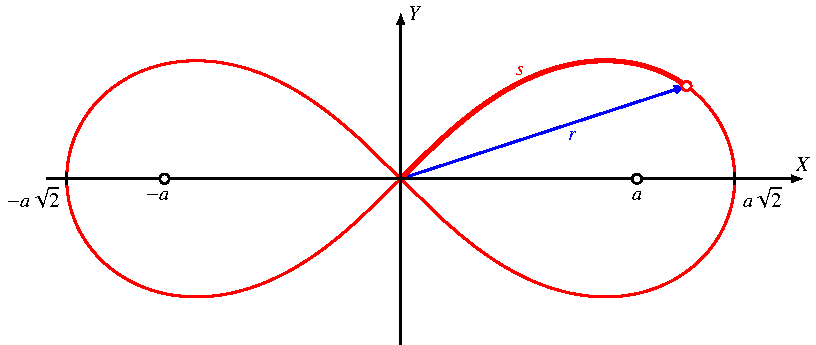
\includegraphics{chapters/110-elliptisch/images/lemniskate.pdf}
\caption{Bogenlänge und Radius der Lemniskate von Bernoulli.
\label{buch:elliptisch:fig:lemniskate}}
\end{figure}
Die Lemniskate von Bernoulli ist die Kurve vierten Grades mit der Gleichung
\begin{equation}
(X^2+Y^2)^2 = 2a^2(X^2-Y^2).
\label{buch:elliptisch:eqn:lemniskate}
\end{equation}
Sie ist in Abbildung~\ref{buch:elliptisch:fig:lemniskate}
dargestellt.
Die beiden Scheitel der Lemniskate befinden sich bei $X_s=\pm a\sqrt{2}$.
Dividiert man die Gleichung der Lemniskate durch $X_s^2=4a^4$ entsteht 
\begin{equation}
\biggl(
\biggl(\frac{X}{a\sqrt{2}}\biggr)^2
+
\biggl(\frac{Y}{a\sqrt{2}}\biggr)^2
\biggr)^2
=
2\frac{a^2}{2a^2}\biggl(
\biggl(\frac{X}{a\sqrt{2}}\biggr)^2
-
\biggl(\frac{Y}{a\sqrt{2}}\biggr)^2
\biggr).
\qquad
\Leftrightarrow
\qquad
(x^2+y^2)^2 = x^2-y^2,
\label{buch:elliptisch:eqn:lemniskatenormiert}
\end{equation}
wobei wir $x=X/a\sqrt{2}$ und $y=Y/a\sqrt{2}$ gesetzt haben.
In dieser Normierung liegen die Scheitel bei $\pm 1$.
Dies ist die Skalierung, die für die Definition des lemniskatischen
Sinus und Kosinus verwendet werden soll.

In Polarkoordinaten $x=r\cos\varphi$ und $y=r\sin\varphi$
gilt nach Einsetzen in \eqref{buch:elliptisch:eqn:lemniskatenormiert}
\begin{equation}
r^4
=
r^2(\cos^2\varphi-\sin^2\varphi)
=
r^2\cos2\varphi
\qquad\Rightarrow\qquad
r^2 = \cos 2\varphi
\label{buch:elliptisch:eqn:lemniskatepolar}
\end{equation}
als Darstellung der Lemniskate in Polardarstellung.
Sie gilt für Winkel $\varphi\in[-\frac{\pi}4,\frac{\pi}4]$ für das
rechte Blatt und $\varphi\in[\frac{3\pi}4,\frac{5\pi}4]$ für das linke
Blatt der Lemniskate.

\subsection{Bogenlänge}
Die Funktionen
\begin{equation}
x(r) = \frac{r}{\sqrt{2}}\sqrt{1+r^2},
\quad
y(r) = \frac{r}{\sqrt{2}}\sqrt{1-r^2}
\label{buch:geometrie:eqn:lemniskateparam}
\end{equation}
erfüllen
\begin{align*}
x(r)^2-y(r)^2
&=
\frac{r^2(1+r^2)}{2}-\frac{r^2(1-r^2)}{2}
\\
&
=
r^4
=
(x(r)^2 + y(r)^2)^2,
\end{align*}
sie stellen also eine Parametrisierung der Lemniskate dar.

Mit Hilfe der Parametrisierung~\eqref{buch:geometrie:eqn:lemniskateparam}
kann man die Länge $s$ des in Abbildung~\ref{buch:elliptisch:fig:lemniskate}
dargestellten Bogens der Lemniskate berechnen.
Dazu benötigt man die Ableitungen nach $r$, die man mit der Produkt- und
Kettenregel berechnen kann:
\begin{align*}
\dot{x}(r)
&=
\frac{\sqrt{1+r^2}}{\sqrt{2}}
+
\frac{r^2}{\sqrt{2}\sqrt{1+r^2}}
&&\Rightarrow&
\dot{x}(r)^2
&=
\frac{1+r^2}{2} +r^2 + \frac{r^4}{2(1+r^2)}
\\
\dot{y}(r)
&=
\frac{\sqrt{1-r^2}}{\sqrt{2}}
-
\frac{r^2}{\sqrt{2}\sqrt{1-r^2}}
&&\Rightarrow&
\dot{y}(r)^2
&=
\frac{1-r^2}{2} -r^2 + \frac{r^4}{2(1-r^2)}
\end{align*}
Die Summe der Quadrate ist
\begin{align*}
\dot{x}(r)^2 + \dot{y}(r)^2
&=
1 + r^4\frac{1-r^2+1+r^2}{2(1+r^2)(1-r^2)}
=
1+r^4\frac{2}{2(1-r^4)}
=
\frac{1-r^4+r^4}{1-r^4}
=
\frac1{1-r^4}.
\end{align*}
Durch Einsetzen in das Integral für die Bogenlänge bekommt man
\begin{equation}
s(r)
=
\int_0^r
\frac{1}{\sqrt{1-t^4}}\,dt.
\label{buch:elliptisch:eqn:lemniskatebogenlaenge}
\end{equation}

%
% Als elliptisches Integral
%
\subsection{Darstellung als elliptisches Integral}
Das unvollständige elliptische Integral erster Art mit Parameter
$k^2=-1$ oder $k=i$ ist
\[
K(r,i)
=
\int_0^x \frac{dt}{\sqrt{(1-t^2)(1-i^2 t^2)}}
=
\int_0^x \frac{dt}{\sqrt{(1-t^2)(1-(-1)t^2)}}
=
\int_0^x \frac{dt}{\sqrt{1-t^4}}
=
s(r).
\]
Der lemniskatische Sinus ist also eine Umkehrfunktion des
elliptischen Integrals erster Art für den speziellen Wert $i$ des
Parameters $k$.

Die Länge des rechten Blattes der Lemniskate wird mit $\varpi$ bezeichnet
und hat den numerischen Wert
\[
\varpi
=
2\int_0^1\sqrt{\frac{1}{1-t^4}}\,dt
=
2.6220575542.
\]
$\varpi$ ist auch als die {\em lemniskatische Konstante} bekannt.
\index{lemniskatische Konstante}%
Der Lemniskatenbogen zwischen dem Nullpunkt und $(1,0)$ hat die Länge
$\varpi/2$.

%
%  Bogenlängenparametrisierung
%
\subsection{Bogenlängenparametrisierung}
Die Lemniskate mit der Gleichung
\[
(X^2+X^2)^2=2(X^2-X^2)
\]
(der Fall $a=1$ in \eqref{buch:elliptisch:eqn:lemniskate})
kann mit Jacobischen elliptischen Funktionen
parametrisiert werden.
Dazu schreibt man
\[
\left.
\begin{aligned}
X(t)
&=
\sqrt{2}\operatorname{cn}(t,k) \operatorname{dn}(t,k)
\\
Y(t)
&=
\phantom{\sqrt{2}}
\operatorname{cn}(t,k) \operatorname{sn}(t,k)
\end{aligned}
\quad\right\}
\qquad\text{mit $k=\displaystyle\frac{1}{\sqrt{2}}$}
\]
und berechnet die beiden Seiten der definierenden Gleichung der
Lemniskate.
Zunächst ist
\begin{align*}
X(t)^2
&=
2\operatorname{cn}(t,k)^2
\operatorname{dn}(t,k)^2
\\
Y(t)^2
&=
\operatorname{cn}(t,k)^2
\operatorname{sn}(t,k)^2
\\
X(t)^2+Y(t)^2
&=
2\operatorname{cn}(t,k)^2
\bigl(
\underbrace{
\operatorname{dn}(t,k)^2
+{\textstyle\frac12}
\operatorname{sn}(t,k)^2
}_{\displaystyle =1}
\bigr)
%\\
%&
=
2\operatorname{cn}(t,k)^2
\\
X(t)^2-Y(t)^2
&=
\operatorname{cn}(t,k)^2
\bigl(
2\operatorname{dn}(t,k)^2 - \operatorname{sn}(t,k)^2
\bigr)
\\
&=
\operatorname{cn}(t,k)^2
\bigl(
2\bigl({\textstyle\frac12}+{\textstyle\frac12}\operatorname{cn}(t,k)^2\bigr)
-
\bigl(1-\operatorname{cn}(t,k)^2\bigr)
\bigr)
\\
&=
2\operatorname{cn}(t,k)^4
\\
\Rightarrow\qquad
(X(t)^2+Y(t)^2)^2
&=
4\operatorname{cn}(t,k)^4
=
2(X(t)^2-Y(t)^2).
\end{align*}
Wir zeigen jetzt, dass dies tatsächlich eine Bogenlängenparametrisierung
der Lemniskate ist.
Dazu berechnen wir die Ableitungen
\begin{align*}
\dot{X}(t)
&=
\sqrt{2}\operatorname{cn}'(t,k)\operatorname{dn}(t,k)
+
\sqrt{2}\operatorname{cn}(t,k)\operatorname{dn}'(t,k)
\\
&=
-\sqrt{2}\operatorname{sn}(t,k)\operatorname{dn}(t,k)^2
-\frac12\sqrt{2}\operatorname{sn}(t,k)\operatorname{cn}(t,k)^2
\\
&=
-\sqrt{2}\operatorname{sn}(t,k)\bigl(
1-{\textstyle\frac12}\operatorname{sn}(t,k)^2
+{\textstyle\frac12}-{\textstyle\frac12}\operatorname{sn}(u,t)^2
\bigr)
\\
&=
\sqrt{2}\operatorname{sn}(t,k)
\bigl(
{\textstyle \frac32}-\operatorname{sn}(t,k)^2
\bigr)
\\
\dot{X}(t)^2
&=
2\operatorname{sn}(t,k)^2
\bigl(
{\textstyle \frac32}-\operatorname{sn}(t,k)^2
\bigr)^2
\\
&=
{\textstyle\frac{9}{2}}\operatorname{sn}(t,k)^2
-
6\operatorname{sn}(t,k)^4
+2\operatorname{sn}(t,k)^6
\\
\dot{Y}(t)
&=
\operatorname{cn}'(t,k)\operatorname{sn}(t,k)
+
\operatorname{cn}(t,k)\operatorname{sn}'(t,k)
\\
&=
-\operatorname{sn}(t,k)^2
\operatorname{dn}(t,k)
+\operatorname{cn}(t,k)^2
\operatorname{dn}(t,k)
\\
&=
\operatorname{dn}(t,k)\bigl(1-2\operatorname{sn}(t,k)^2\bigr)
\\
\dot{Y}(t)^2
&=
\bigl(1-{\textstyle\frac12}\operatorname{sn}(t,k)^2\bigr)
\bigl(1-2\operatorname|{sn}(t,k)^2\bigr)^2
\\
&=
1-{\textstyle\frac{9}{2}}\operatorname{sn}(t,k)^2
+6\operatorname{sn}(t,k)^4
-2\operatorname{sn}(t,k)^6
\\
\dot{X}(t)^2 + \dot{Y}(t)^2
&=
1.
\end{align*}
Dies bedeutet, dass die Bogenlänge zwischen den Parameterwerten $0$ und $s$
\[
\int_0^s
\sqrt{\dot{X}(t)^2 + \dot{Y}(t)^2}
\,dt
=
\int_0^s\,dt
=
s,
\]
der Parameter $t$ ist also ein Bogenlängenparameter.

Die mit dem Faktor $1/\sqrt{2}$ skalierte Standard-Lemniskate mit der
Gleichung
\[
(x^2+y^2)^2 = x^2-y^2
\]
hat daher eine Bogenlängenparametrisierung mit
\begin{equation}
\begin{aligned}
x(t)
&=
\phantom{\frac{1}{\sqrt{2}}}
\operatorname{cn}(\sqrt{2}t,k)\operatorname{dn}(\sqrt{2}t,k)
\\
y(t)
&=
\frac{1}{\sqrt{2}}\operatorname{cn}(\sqrt{2}t,k)\operatorname{sn}(\sqrt{2}t,k)
\end{aligned}
\label{buch:elliptisch:lemniskate:bogenlaenge}
\end{equation}

\subsection{Der lemniskatische Sinus und Kosinus}
Der Sinus Berechnet die Gegenkathete zu einer gegebenen Bogenlänge des
Kreises, er ist die Umkehrfunktion der Funktion, die der Gegenkathete
die Bogenlänge zuordnet.

Daher ist es naheliegend, die Umkehrfunktion von $s(r)$ in 
\eqref{buch:elliptisch:eqn:lemniskatebogenlaenge}
den {\em lemniskatischen Sinus} zu nennen mit der Bezeichnung
$r=\operatorname{sl} s$.

Der Kosinus ist der Sinus des komplementären Winkels.
Auch für die lemniskatische Bogenlänge $s(r)$ lässt sich eine
komplementäre Bogenlänge definieren, nämlich die Bogenlänge zwischen
dem Punkt $(x(r), y(r))$ und $(1,0)$.

Da die Parametrisierung~\eqref{buch:elliptisch:lemniskate:bogenlaenge}
eine Bogenlängenparametrisierung ist, darf man $t=s$ schreiben.
Dann kann man aber auch $r(s)$ daraus berechnen,
es ist
\[
r(s)^2
=
x(s)^2 + y(s)^2
=
\operatorname{cn}(s\sqrt{2},k)^2
\qquad\Rightarrow\qquad
r(s)
=
\operatorname{cn}(s\sqrt{2},k)
\]

\begin{figure}
\centering
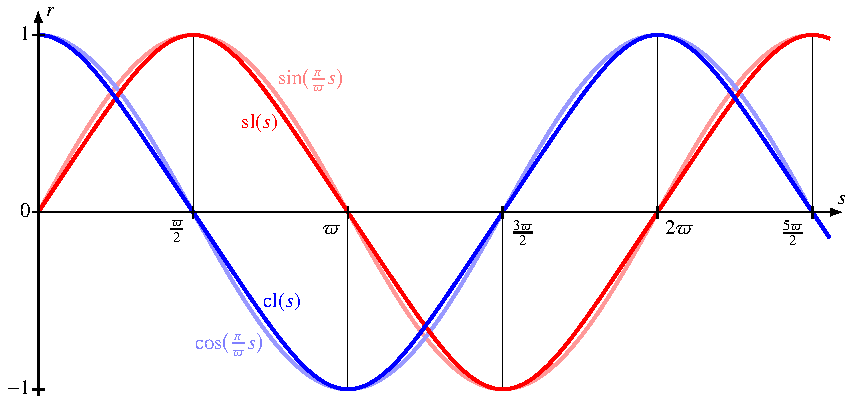
\includegraphics{chapters/110-elliptisch/images/slcl.pdf}
\caption{
Lemniskatischer Sinus und Kosinus sowie Sinus und Kosinus
mit derart skaliertem Argument, dass die Funktionen die gleichen Nullstellen
haben.
\label{buch:elliptisch:figure:slcl}}
\end{figure}


%\section*{Übungsaufgaben}
%\rhead{Übungsaufgaben}
%\aufgabetoplevel{chapters/020-exponential/uebungsaufgaben}
%\begin{uebungsaufgaben}
%\uebungsaufgabe{0}
%\uebungsaufgabe{1}
%\end{uebungsaufgaben}


%
% chapter.tex -- Beschreibung des Inhaltes
%
% (c) 2021 Prof Dr Andreas Müller, Hochschule Rapperswil
%
% !TeX spellcheck = de_CH
\chapter{Elliptische Funktionen
\label{buch:chapter:geometrie}}
\lhead{Elliptische Funktionen}
\rhead{}

Der Versuch, die Länge eines Ellipsenbogens zu berechnen, hat
in Abschnitt~\ref{buch:geometrie:subsection:hyperbeln-und-ellipsen}
zu Integralen geführt, die nicht in geschlossener Form ausgewertet
werden können.
Neben den dort gefundenen Integralen sind noch weitere, ähnlich
aufgebaute Integrale in dieser Familie zu finden.

%
% ellintegral.tex
%
% (c) 2021 Prof Dr Andreas Müller, OST Ostschweizer Fachhochschule
%
\section{Elliptische Integrale
\label{buch:elliptisch:section:integral}}
\rhead{Elliptisches Integral}
Bei der Berechnung des Ellipsenbogens in 
Abschnitt~\ref{buch:geometrie:subsection:hyperbeln-und-ellipsen}
sind wir auf ein Integral gestossen, welches sich nicht in geschlossener
Form ausdrücken liess.
Um solche Integrale in den Griff zu bekommen, ist es nötig, sie als
neue spezielle Funktionen zu definieren.

\subsection{Definition
\label{buch:elliptisch:subsection:definition}}
Ein {\em elliptisches Integral} ist ein Integral der Form
\index{elliptishes Integral}%
\index{Integral, elliptisch}%
\begin{equation}
\int R\left( x, \sqrt{p(x)}\right)\,dx
\label{buch:elliptisch:def:allgemein}
\end{equation}
wobei $R(x,y)$ eine rationale Funktion von zwei Variablen ist und
$p(x)$ ein Polynom dritten oder vierten Grades.
Hätte $p(x)$ ein mehrfache Nullstelle $x_0$, müsste es durch $(x-x_0)^2$
teilbar sein, man könnte also einen Faktor $(x-x_0)$ aus der
Wurzel im Integraneden von \eqref{buch:elliptisch:def:allgemein}
ausklammern und damit das Integral in eine Form bringen, wo $p(x)$
höchstens zweiten Grades ist.
Solche Integrale lassen sich meistens mit trigonometrischen Substitutionen
berechnen.
Wir verlangen daher, dass $p(x)$ keine mehrfachen Nullstellen hat.

Man kann zeigen, dass sich elliptische Integrale in Summen von
elementaren Funktionen und speziellen elliptischen Integralen 
der folgenden Form überführen lassen
\cite[Abschnitt 164, p.~506]{buch:smirnov32}.

\begin{definition}
\label{buch:elliptisch:def:integrale123}
Die elliptischen Integrale erster, zweiter und dritter Art sind die
Integrale
\[
\begin{aligned}
\text{1.~Art:}&&&
\int \frac{dx}{\sqrt{(1-x^2)(1-k^2x^2)}}
\\
\text{2.~Art:}&&&
\int \sqrt{\frac{1-k^2x^2}{1-x^2}}\,dx
\\
\text{3.~Art:}&&&
\int \frac{dx}{(1-nx^2)\sqrt{(1-x^2)(1-k^2x^2)}}
\end{aligned}
\]
mit $0<k<1$.
Es ist auch üblich, den Parameter $m=k^2$ zu verwenden.
\end{definition}

Wie gesagt lassen sich für diese unbestimmten Integrale keine 
geschlossenen Formen finden.
Es bleibt uns daher nichts anderes übrig, als die Integralgrenzen
festzulegen und damit eine Stammfunktion auszuwählen.

%
% Elliptisches Integral
%
\subsection{Vollständige elliptische Integrale
\label{buch:elliptisch:subsection:vollstaendig}}
In diesem Abschnitt legen wir beide Integrationsgrenzen fest und
untersuchen die entstehenenden Funktionen von den Parametern
$k$ und $n$.

\subsubsection{Definition der vollständigen elliptischen Integrale}
Da der Nenner in allen drei elliptischen Integralen eine Nullstelle
bei $\pm1$ hat, kann das Integral nur von $0$ bis $1$ erstreckt werden.

\begin{definition}
\label{buch:elliptisch:def:vollstintegrale123}
Die vollständigen elliptischen Integrale erster, zweiter und dritter
Art sind
\[
\begin{aligned}
\text{1.~Art:}&&
K(k)&=\int_0^1 \frac{dt}{\sqrt{(1-t^2)(1-k^2t^2)}} \\
\text{2.~Art:}&&
E(k)&=\int_0^1 \sqrt{\frac{1-k^2t^2}{1-t^2}}\,dt \\
\text{3.~Art:}&&
\Pi(n, k)&=\int_0^1\frac{dt}{(1-nt^2)\sqrt{(1-t^2)(1-k^2t^2)}} 
\end{aligned}
\]
mit $0<k<1$.
\end{definition}

Die Funktionen hängen stetig von $k$ ab.
Die Nullstellen des Faktors $1-k^2x^2$ liegen ausserhalb des
Integrationsintervalls und spielen daher keine Rolle.
Die Werte von $K(k)$ und $E(k)$ für $k=0$ können direkt berechnet
werden:
\begin{align*}
K(0)
=
E(0)
&=
\int_0^1 \frac{dt}{\sqrt{1-t^2}}=\frac{\pi}2.
\end{align*}
Das Integral $\Pi(n,0)$ ist etwas komplizierter.

Für $k\to 1$ ist $E(k)=1$, die Integrale $K(1)$ und $\Pi(n,1)$
sind dagegen divergent.

\subsubsection{Jacobi- und Legendre-Normalform}
Die Integrationsvariable $t$ der vollständigen elliptischen Integrale
kann durch die Substitution $t=\sin\varphi$ durch die Variable
$\varphi$ und das Integral über das Intervall $[0,1]$ durch ein
Integral über das Intervall $[0,\frac{\pi}2]$ ersetzt werden.
Mit
\[
\frac{dt}{d\varphi} = \cos\varphi = \sqrt{1-\sin^2\varphi}
\]
können die Funktionen $K(k)$, $E(k)$ und $\Pi(n,k)$ auch als
\begin{align*}
K(k)
&=
\int_0^{\frac{\pi}2}
\frac{
\sqrt{1-\sin^2\varphi}\,d\varphi
}{
\sqrt{(1-\sin^2\varphi)(1-k^2\sin^2\varphi)}
}
=
\int_0^{\frac{\pi}2}
\frac{d\varphi}{\sqrt{1-k^2\sin^2\varphi}}
\\
E(k)
&=
\int_0^{\frac{\pi}2}
\sqrt{\frac{1-k^2\sin^2\varphi}{1-\sin^2\varphi}}\sqrt{1-\sin^2\varphi}\,d\varphi
=
\int_0^{\frac{\pi}2}
\sqrt{1-k^2\sin^2\varphi}\,d\varphi
\\
\Pi(n,k)
&=
\int_0^{\frac{\pi}2}
\frac{
\sqrt{1-\sin^2\varphi}\,d\varphi
}{
(1-n\sin^2\varphi)\sqrt{(1-\sin^2\varphi)(1-k^2\sin^2\varphi)}
}
=
\int_0^{\frac{\pi}2}
\frac{
d\varphi
}{
(1-n\sin^2\varphi)\sqrt{1-k^2\sin^2\varphi}
}
\end{align*}
Diese Form wird auch die {\em Legendre-Normalform} der vollständigen 
\index{Legendre-Normalform}%
elliptischen Integrale genannt, während die Form von
Definition~\ref{buch:elliptisch:def:vollstintegrale123}
die {\em Jacobi-Normalform} heisst.
\index{Jacobi-Normalform}%

\subsubsection{Umfang einer Ellipse}
\begin{figure}
\centering
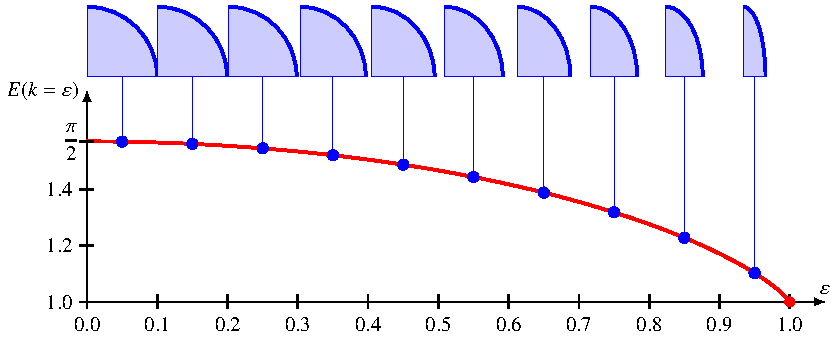
\includegraphics{chapters/110-elliptisch/images/ellipsenumfang.pdf}
\caption{Bogenlänge eines Viertels einer Ellipse mit Exzentrizität
$\varepsilon$.
\label{buch:elliptisch:fig:ellipsenumfang}}
\end{figure}
Wir zeigen, wie sich die Berechnung des Umfangs $U$ einer Ellipse
mit Halbachsen $a$ und $b$, $a\le b$, auf ein volltändiges elliptisches
Integral zurückführen lässt.
Der Fall $a>b$ kann behandelt werden, indem die $x$- und $y$-Koordinaten
vertauscht werden.

Die Parametrisierung
\[
t\mapsto \begin{pmatrix}a\cos t\\ b\sin t\end{pmatrix}
\]
einer Ellipse führt auf das Integral
\begin{align*}
U
&=
\int_0^{2\pi} \sqrt{a^2\sin^2t + b^2\cos^2 t}\,dt
\notag
\\
&=
4\int_0^{\frac{\pi}2}
\sqrt{a^2\sin^2t + b^2(1-\sin^2 t)}
\,dt
\notag
\\
&=
4b \int_0^{\frac{\pi}2} \sqrt{1-(b^2-a^2)/b^2\cdot \sin^2t}\,dt
\label{buch:elliptisch:eqn:umfangellipse}
\end{align*}
für den Umfang der Ellipse.
Bei einem Kreis ist $a=b$ und der zweite Term unter der Wurzel fällt weg,
der Umfang wird $4b\frac{\pi}2=2\pi b$.
Die Differenz $e^2=b^2-a^2$ ist die {\em lineare Exzentrizität} der Ellipse,
\index{lineare Exzentrizität}%
der Quotient $e/b$ wird die {\em numerische Exzentrizität} der Ellipse
genannt.
Insbesondere ist $k = \varepsilon$.

Das Integral~\eqref{buch:elliptisch:eqn:umfangellipse} erhält jetzt die
Form
\[
U
=
4b\int_0^{\frac{\pi}2} \sqrt{1-k^2\sin^2t}\,dt
\]
und ist damit als elliptisches Integral zweiter Art erkannt.
Für den Umfang der Ellipse finden wir damit die Formel
\[
U
=
4b E(k)
=
4b E(\varepsilon).
\]
Das vollständige elliptische Integral zweiter Art $E(\varepsilon)$
liefert also genau den Umfang der eines Viertels Ellipse mit
numerischer Exzentrizität $\varepsilon$ und kleiner Halbachse $1$.

\subsubsection{Komplementäre Integrale}
XXX Komplementäre Integrale \\

\subsubsection{Ableitung}
XXX Ableitung \\
XXX Stammfunktion \\

\subsection{Unvollständige elliptische Integrale}
XXX Vollständige und Unvollständige Integrale \\
XXX Additionstheoreme \\
XXX Parameterkonventionen \\

\subsection{Potenzreihe}
XXX Potenzreihen \\
XXX Als hypergeometrische Funktionen \\



\section{Jacobische elliptische Funktionen}

Für das elliptische Filter werden, wie es der Name bereits deutet, elliptische Funktionen gebraucht.
Wie die trigonometrischen Funktionen Zusammenhänge eines Kreises darlegen, beschreiben die elliptischen Funktionen Ellipsen.
Es ist daher naheliegend, dass der Kosinus des Tschebyscheff-Filters gegen ein elliptisches Pendant ausgetauscht werden könnte.
Der Begriff elliptische Funktion wird für sehr viele Funktionen gebraucht, daher ist es hier wichtig zu erwähnen, dass es ausschliesslich um die Jacobischen elliptischen Funktionen geht.

\subsection{Grundlegende Eigenschaften}

Die Jacobi elliptischen Funktionen werden ausführlich im Kapitel \ref{buch:elliptisch:section:jacobi} behandelt.
Im Wesentlichen erweitern die Jacobi elliptischen Funktionen die trigonometrische Funktionen für Ellipsen.
Zum Beispiel gibt es analog zum Sinus den elliptischen $\sn(z, k)$.
Im Gegensatz zum den trigonometrischen Funktionen haben die elliptischen Funktionen zwei Parameter.
Den \textit{elliptische Modul} $k$, der die Exzentrizität der Ellipse parametrisiert und das Winkelargument $z$.
Im Kreis ist der Radius für alle Winkel konstant, bei Ellipsen ändert sich das.
Dies hat zur Folge, dass bei einer Ellipse die Kreisbogenlänge nicht linear zum Winkel verläuft.
Darum kann hier nicht der gewohnte Winkel verwendet werden.
Das Winkelargument $z$ kann durch das elliptische Integral erster Art
\begin{equation}
    z
    =
    F(\phi, k)
    =
    \int_{0}^{\phi}
    \frac{
        d\theta
    }{
        \sqrt{
            1-k^2 \sin^2 \theta
        }
    }
\end{equation}
mit dem Winkel $\phi$ in Verbindung gebracht werden.

Dabei wird das vollständige und unvollständige elliptische integral unterschieden.
Beim vollständigen Integral
\begin{equation}
    K(k)
    =
    \int_{0}^{\pi / 2}
    \frac{
        d\theta
    }{
        \sqrt{
            1-k^2 \sin^2 \theta
        }
    }
\end{equation}
wird über ein viertel Ellipsenbogen integriert, also bis $\phi=\pi/2$ und liefert das Winkelargument für eine Vierteldrehung.
Die Zahl wird oft auch abgekürzt mit $K = K(k)$ und ist für das elliptische Filter sehr relevant.
Alle elliptischen Funktionen sind somit $4K$-periodisch.

Neben dem $\sn$ gibt es zwei weitere elliptische Basisfunktionen $\cn$ und $\dn$.
Dazu kommen noch weitere abgeleitete Funktionen, die durch Quotienten und Kehrwerte dieser Funktionen zustande kommen.
Insgesamt sind es die zwölf Funktionen
\begin{equation*}
    \sn \quad
    \ns \quad
    \scelliptic \quad
    \sd \quad
    \cn \quad
    \nc \quad
    \cs \quad
    \cd \quad
    \dn \quad
    \nd \quad
    \ds \quad
    \dc.
\end{equation*}

Die Jacobischen elliptischen Funktionen können mit der inversen Funktion des vollständigen elliptischen Integrals erster Art
\begin{equation}
    \phi = F^{-1}(z, k)
\end{equation}
definiert werden. Dabei ist zu beachten dass nur das $z$ Argument der Funktion invertiert wird, also
\begin{equation}
    z = F(\phi, k)
    \Leftrightarrow
    \phi = F^{-1}(z, k).
\end{equation}
Mithilfe von $F^{-1}$ kann zum Beispiel $sn^{-1}$ mit dem elliptischen Integral dargestellt werden:
\begin{equation}
    \sin(\phi)
    =
    \sin \left( F^{-1}(z, k) \right)
    =
    \sn(z, k)
    =
    w.
\end{equation}

% \begin{equation} %TODO remove unnecessary equations
%     \phi
%     =
%      F^{-1}(z, k)
%      =
%      \sin^{-1} \big( \sn (z, k ) \big)
%      =
%     \sin^{-1} ( w )
% \end{equation}

% \begin{equation}
%     F(\phi, k)
%     =
%     z
%     =
%     F( \sin^{-1} \big( \sn (z, k ) \big) , k)
%     =
%     F( \sin^{-1} ( w ), k)
% \end{equation}

% \begin{equation}
%     \sn^{-1}(w, k)
%     =
%     F(\phi, k),
%     \quad
%     \phi = \sin^{-1}(w)
% \end{equation}

\subsection{Die Funktion $\sn^{-1}$}

Beim Tschebyscheff-Filter konnten wir mit Betrachten des Arcuscosinus die Funktionalität erklären.
Für das Elliptische Filter machen wir die gleiche Betrachtung mit der $\sn^{-1}$-Funktion.
Der $\sn^{-1}$ ist durch das elliptische Integral
\begin{align}
    \sn^{-1}(w, k)
        & =
    \int_{0}^{\phi}
    \frac{
        d\theta
    }{
        \sqrt{
            1-k^2 \sin^2 \theta
        }
    },
    \quad
    \phi = \sin^{-1}(w)
    \\
        & =
    \int_{0}^{w}
    \frac{
        dt
    }{
        \sqrt{
            (1-t^2)(1-k^2 t^2)
        }
    }
\end{align}
beschrieben.
Dazu betrachten wir wieder den Integranden
\begin{equation}
    \frac{
        1
    }{
        \sqrt{
            (1-t^2)(1-k^2 t^2)
        }
    }.
\end{equation}
Beim $\cos^{-1}(x)$ haben wir gesehen, dass die analytische Fortsetzung bei $x < -1$ und $x > 1$ rechtwinklig in die komplexen Zahlen wandert.
Wenn man das Gleiche mit $\sn^{-1}(w, k)$ macht, erkennt man zwei interessante Stellen.
Die erste ist die gleiche wie beim $\cos^{-1}(x)$ nämlich bei $t = \pm 1$.
Der erste Term unter der Wurzel wird dann negativ, während der zweite noch positiv ist, da $k \leq 1$.
Ab diesem Punkt knickt die Funktion in die imaginäre Richtung ab.
Bei $t = 1/k$ ist auch der zweite Term negativ und die Funktion verläuft in die negative reelle Richtung.
Abbildung \ref{ellfilter:fig:sn} zeigt den Verlauf der Funktion in der komplexen Ebene.
\begin{figure}
    \centering
    \begin{tikzpicture}[>=stealth', auto, node distance=2cm, scale=1.2]

    \tikzstyle{zero} = [draw, circle, inner sep =0, minimum height=0.15cm]

    \tikzset{pole/.style={cross out, draw=black, minimum size=(0.15cm-\pgflinewidth), inner sep=0pt, outer sep=0pt}}

    \begin{scope}[xscale=0.9, yscale=1.8]

        \draw[gray, ->] (0,-1.5) -- (0,1.5) node[anchor=south]{$\mathrm{Im}~z$};
        \draw[gray, ->] (-5,0) -- (5,0) node[anchor=west]{$\mathrm{Re}~z$};

        \begin{scope}

            \clip(-4.5,-1.25) rectangle (4.5,1.25);

            \fill[yellow!30] (0,0) rectangle (1, 0.5);

            \begin{scope}[xshift=-1cm]

                \foreach \i in {-2,...,2} {
                    \foreach \j in {-2,...,1} {
                        \begin{scope}[xshift=\i*4cm, yshift=\j*1cm]
                            \draw[<-, blue!50] (0, 0) -- (0,0.5);
                            \draw[<-, cyan!50] (1, 0) -- (0,0);
                            \draw[<-, darkgreen!50] (2, 0) -- (1,0);
                            \draw[<-, orange!50] (2,0.5) -- (2, 0);
                            \draw[<-, red!50] (1, 0.5) -- (2,0.5);
                            \draw[<-, purple!50] (0, 0.5) -- (1,0.5);
                            \draw[<-, blue!50] (0,1) -- (0,0.5);
                            \draw[<-, orange!50] (2,0.5) -- (2, 1);
                            \draw[<-, red!50] (3, 0.5) -- (2,0.5);
                            \draw[<-, purple!50] (4, 0.5) -- (3,0.5);
                            \draw[<-, darkgreen!50] (2, 0) -- (3,0);
                            \draw[<-, cyan!50] (3, 0) -- (4,0);
                        \end{scope}
                    }
                }

                % \pause
                \draw[ultra thick, <-, darkgreen] (2, 0) -- (1,0);
                % \pause
                \draw[ultra thick, <-, orange] (2,0.5) -- (2, 0);
                % \pause
                \draw[ultra thick, <-, red] (1, 0.5) -- (2,0.5);
                % \pause
                \draw[ultra thick, <-, blue] (0, 0) -- (0,0.5);
                \draw[ultra thick, <-, purple] (0, 0.5) -- (1,0.5);
                \draw[ultra thick, <-, cyan] (1, 0) -- (0,0);
                % \pause


                \foreach \i in {-2,...,2} {
                    \foreach \j in {-2,...,1} {
                        \begin{scope}[xshift=\i*4cm, yshift=\j*1cm]
                            \node[zero] at ( 1, 0) {};
                            \node[zero] at ( 3, 0) {};
                            \node[pole] at ( 1,0.5) {};
                            \node[pole] at ( 3,0.5) {};
                        \end{scope}
                    }
                }

            \end{scope}

        \end{scope}

        \draw[gray] ( 1,0) +(0,0.1) -- +(0, -0.1) node[inner sep=0, anchor=north] {\small $K$};
        \draw[gray]  (0, 0.5) +(0.1, 0) -- +(-0.1, 0) node[inner sep=0, anchor=east]{\small $jK^\prime$};

    \end{scope}

    \node[zero] at (4,3) (n) {};
    \node[anchor=west] at (n.east) {Zero};
    \node[pole, below=0.25cm of n] (n) {};
    \node[anchor=west] at (n.east) {Pole};

    \begin{scope}[yshift=-4cm, xscale=0.75]

        \draw[gray, ->] (-6,0) -- (6,0) node[anchor=west]{$w$};

        \draw[ultra thick, ->, purple] (-5, 0) -- (-3, 0);
        \draw[ultra thick, ->, blue]      (-3, 0) -- (-2, 0);
        \draw[ultra thick, ->, cyan]       (-2, 0) -- (0, 0);
        \draw[ultra thick, ->, darkgreen]    (0, 0) -- (2, 0);
        \draw[ultra thick, ->, orange] (2, 0) -- (3, 0);
        \draw[ultra thick, ->, red] (3, 0) -- (5, 0);

        \node[anchor=south] at (-5,0) {$-\infty$};
        \node[anchor=south] at (-3,0) {$-1/k$};
        \node[anchor=south] at (-2,0) {$-1$};
        \node[anchor=south] at (0,0) {$0$};
        \node[anchor=south] at (2,0) {$1$};
        \node[anchor=south] at (3,0) {$1/k$};
        \node[anchor=south] at (5,0) {$\infty$};

    \end{scope}


\end{tikzpicture}
    \caption{
        $z$-Ebene der Funktion $z = \sn^{-1}(w, k)$.
        Die Funktion ist in der realen Achse $4K$-periodisch und in der imaginären Achse $2jK^\prime$-periodisch.
    }
    \label{ellfilter:fig:sn}
\end{figure}
In der reellen Richtung ist sie $4K(k)$-periodisch und in der imaginären Richtung $4K^\prime(k)$-periodisch, wobei $K^\prime$ das komplementäre vollständige Elliptische Integral ist:
\begin{equation}
    K^\prime(k)
    =
    \int_{0}^{\pi / 2}
    \frac{
        d\theta
    }{
        \sqrt{
            1-{k^\prime}^2 \sin^2 \theta
        }
    },
    \quad
    k^\prime = \sqrt{1-k^2}.
\end{equation}

%
% lemniskate.tex
%
% (c) 2021 Prof Dr Andreas Müller, OST Ostschweizer Fachhochschule
%
\section{Lemniskatischer Sinus
\label{buch:elliptisch:section:lemniskate}}
\rhead{Lemniskatischer Sinus}
Historisch war der {\em lemniskatische Sinus} die erste ellptische
Funktion, die Gauss bereits als 19-jähriger untersucht, aber nicht 
veröffentlich hat.
In diesem Abschnitt soll die Verbindung zu den Jacobischen
elliptischen Funktionen hergestellt werden.

\subsection{Lemniskate
\label{buch:gemotrie:subsection:lemniskate}}
\begin{figure}
\centering
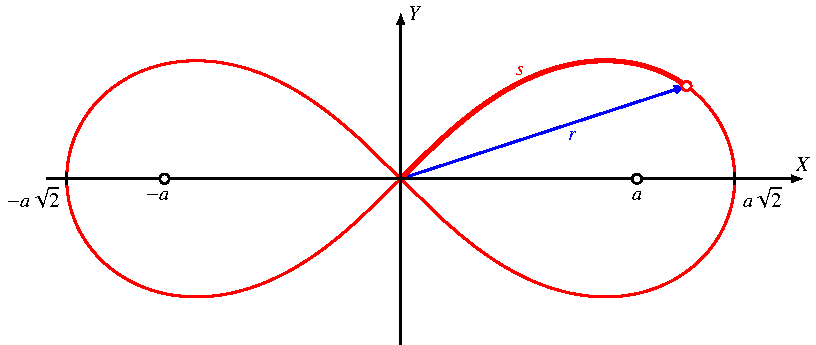
\includegraphics{chapters/110-elliptisch/images/lemniskate.pdf}
\caption{Bogenlänge und Radius der Lemniskate von Bernoulli.
\label{buch:elliptisch:fig:lemniskate}}
\end{figure}
Die Lemniskate von Bernoulli ist die Kurve vierten Grades mit der Gleichung
\begin{equation}
(X^2+Y^2)^2 = 2a^2(X^2-Y^2).
\label{buch:elliptisch:eqn:lemniskate}
\end{equation}
Sie ist in Abbildung~\ref{buch:elliptisch:fig:lemniskate}
dargestellt.
Die beiden Scheitel der Lemniskate befinden sich bei $X_s=\pm a\sqrt{2}$.
Dividiert man die Gleichung der Lemniskate durch $X_s^2=4a^4$ entsteht 
\begin{equation}
\biggl(
\biggl(\frac{X}{a\sqrt{2}}\biggr)^2
+
\biggl(\frac{Y}{a\sqrt{2}}\biggr)^2
\biggr)^2
=
2\frac{a^2}{2a^2}\biggl(
\biggl(\frac{X}{a\sqrt{2}}\biggr)^2
-
\biggl(\frac{Y}{a\sqrt{2}}\biggr)^2
\biggr).
\qquad
\Leftrightarrow
\qquad
(x^2+y^2)^2 = x^2-y^2,
\label{buch:elliptisch:eqn:lemniskatenormiert}
\end{equation}
wobei wir $x=X/a\sqrt{2}$ und $y=Y/a\sqrt{2}$ gesetzt haben.
In dieser Normierung liegen die Scheitel bei $\pm 1$.
Dies ist die Skalierung, die für die Definition des lemniskatischen
Sinus und Kosinus verwendet werden soll.

In Polarkoordinaten $x=r\cos\varphi$ und $y=r\sin\varphi$
gilt nach Einsetzen in \eqref{buch:elliptisch:eqn:lemniskatenormiert}
\begin{equation}
r^4
=
r^2(\cos^2\varphi-\sin^2\varphi)
=
r^2\cos2\varphi
\qquad\Rightarrow\qquad
r^2 = \cos 2\varphi
\label{buch:elliptisch:eqn:lemniskatepolar}
\end{equation}
als Darstellung der Lemniskate in Polardarstellung.
Sie gilt für Winkel $\varphi\in[-\frac{\pi}4,\frac{\pi}4]$ für das
rechte Blatt und $\varphi\in[\frac{3\pi}4,\frac{5\pi}4]$ für das linke
Blatt der Lemniskate.

\subsection{Bogenlänge}
Die Funktionen
\begin{equation}
x(r) = \frac{r}{\sqrt{2}}\sqrt{1+r^2},
\quad
y(r) = \frac{r}{\sqrt{2}}\sqrt{1-r^2}
\label{buch:geometrie:eqn:lemniskateparam}
\end{equation}
erfüllen
\begin{align*}
x(r)^2-y(r)^2
&=
\frac{r^2(1+r^2)}{2}-\frac{r^2(1-r^2)}{2}
\\
&
=
r^4
=
(x(r)^2 + y(r)^2)^2,
\end{align*}
sie stellen also eine Parametrisierung der Lemniskate dar.

Mit Hilfe der Parametrisierung~\eqref{buch:geometrie:eqn:lemniskateparam}
kann man die Länge $s$ des in Abbildung~\ref{buch:elliptisch:fig:lemniskate}
dargestellten Bogens der Lemniskate berechnen.
Dazu benötigt man die Ableitungen nach $r$, die man mit der Produkt- und
Kettenregel berechnen kann:
\begin{align*}
\dot{x}(r)
&=
\frac{\sqrt{1+r^2}}{\sqrt{2}}
+
\frac{r^2}{\sqrt{2}\sqrt{1+r^2}}
&&\Rightarrow&
\dot{x}(r)^2
&=
\frac{1+r^2}{2} +r^2 + \frac{r^4}{2(1+r^2)}
\\
\dot{y}(r)
&=
\frac{\sqrt{1-r^2}}{\sqrt{2}}
-
\frac{r^2}{\sqrt{2}\sqrt{1-r^2}}
&&\Rightarrow&
\dot{y}(r)^2
&=
\frac{1-r^2}{2} -r^2 + \frac{r^4}{2(1-r^2)}
\end{align*}
Die Summe der Quadrate ist
\begin{align*}
\dot{x}(r)^2 + \dot{y}(r)^2
&=
1 + r^4\frac{1-r^2+1+r^2}{2(1+r^2)(1-r^2)}
=
1+r^4\frac{2}{2(1-r^4)}
=
\frac{1-r^4+r^4}{1-r^4}
=
\frac1{1-r^4}.
\end{align*}
Durch Einsetzen in das Integral für die Bogenlänge bekommt man
\begin{equation}
s(r)
=
\int_0^r
\frac{1}{\sqrt{1-t^4}}\,dt.
\label{buch:elliptisch:eqn:lemniskatebogenlaenge}
\end{equation}

%
% Als elliptisches Integral
%
\subsection{Darstellung als elliptisches Integral}
Das unvollständige elliptische Integral erster Art mit Parameter
$k^2=-1$ oder $k=i$ ist
\[
K(r,i)
=
\int_0^x \frac{dt}{\sqrt{(1-t^2)(1-i^2 t^2)}}
=
\int_0^x \frac{dt}{\sqrt{(1-t^2)(1-(-1)t^2)}}
=
\int_0^x \frac{dt}{\sqrt{1-t^4}}
=
s(r).
\]
Der lemniskatische Sinus ist also eine Umkehrfunktion des
elliptischen Integrals erster Art für den speziellen Wert $i$ des
Parameters $k$.

Die Länge des rechten Blattes der Lemniskate wird mit $\varpi$ bezeichnet
und hat den numerischen Wert
\[
\varpi
=
2\int_0^1\sqrt{\frac{1}{1-t^4}}\,dt
=
2.6220575542.
\]
$\varpi$ ist auch als die {\em lemniskatische Konstante} bekannt.
\index{lemniskatische Konstante}%
Der Lemniskatenbogen zwischen dem Nullpunkt und $(1,0)$ hat die Länge
$\varpi/2$.

%
%  Bogenlängenparametrisierung
%
\subsection{Bogenlängenparametrisierung}
Die Lemniskate mit der Gleichung
\[
(X^2+X^2)^2=2(X^2-X^2)
\]
(der Fall $a=1$ in \eqref{buch:elliptisch:eqn:lemniskate})
kann mit Jacobischen elliptischen Funktionen
parametrisiert werden.
Dazu schreibt man
\[
\left.
\begin{aligned}
X(t)
&=
\sqrt{2}\operatorname{cn}(t,k) \operatorname{dn}(t,k)
\\
Y(t)
&=
\phantom{\sqrt{2}}
\operatorname{cn}(t,k) \operatorname{sn}(t,k)
\end{aligned}
\quad\right\}
\qquad\text{mit $k=\displaystyle\frac{1}{\sqrt{2}}$}
\]
und berechnet die beiden Seiten der definierenden Gleichung der
Lemniskate.
Zunächst ist
\begin{align*}
X(t)^2
&=
2\operatorname{cn}(t,k)^2
\operatorname{dn}(t,k)^2
\\
Y(t)^2
&=
\operatorname{cn}(t,k)^2
\operatorname{sn}(t,k)^2
\\
X(t)^2+Y(t)^2
&=
2\operatorname{cn}(t,k)^2
\bigl(
\underbrace{
\operatorname{dn}(t,k)^2
+{\textstyle\frac12}
\operatorname{sn}(t,k)^2
}_{\displaystyle =1}
\bigr)
%\\
%&
=
2\operatorname{cn}(t,k)^2
\\
X(t)^2-Y(t)^2
&=
\operatorname{cn}(t,k)^2
\bigl(
2\operatorname{dn}(t,k)^2 - \operatorname{sn}(t,k)^2
\bigr)
\\
&=
\operatorname{cn}(t,k)^2
\bigl(
2\bigl({\textstyle\frac12}+{\textstyle\frac12}\operatorname{cn}(t,k)^2\bigr)
-
\bigl(1-\operatorname{cn}(t,k)^2\bigr)
\bigr)
\\
&=
2\operatorname{cn}(t,k)^4
\\
\Rightarrow\qquad
(X(t)^2+Y(t)^2)^2
&=
4\operatorname{cn}(t,k)^4
=
2(X(t)^2-Y(t)^2).
\end{align*}
Wir zeigen jetzt, dass dies tatsächlich eine Bogenlängenparametrisierung
der Lemniskate ist.
Dazu berechnen wir die Ableitungen
\begin{align*}
\dot{X}(t)
&=
\sqrt{2}\operatorname{cn}'(t,k)\operatorname{dn}(t,k)
+
\sqrt{2}\operatorname{cn}(t,k)\operatorname{dn}'(t,k)
\\
&=
-\sqrt{2}\operatorname{sn}(t,k)\operatorname{dn}(t,k)^2
-\frac12\sqrt{2}\operatorname{sn}(t,k)\operatorname{cn}(t,k)^2
\\
&=
-\sqrt{2}\operatorname{sn}(t,k)\bigl(
1-{\textstyle\frac12}\operatorname{sn}(t,k)^2
+{\textstyle\frac12}-{\textstyle\frac12}\operatorname{sn}(u,t)^2
\bigr)
\\
&=
\sqrt{2}\operatorname{sn}(t,k)
\bigl(
{\textstyle \frac32}-\operatorname{sn}(t,k)^2
\bigr)
\\
\dot{X}(t)^2
&=
2\operatorname{sn}(t,k)^2
\bigl(
{\textstyle \frac32}-\operatorname{sn}(t,k)^2
\bigr)^2
\\
&=
{\textstyle\frac{9}{2}}\operatorname{sn}(t,k)^2
-
6\operatorname{sn}(t,k)^4
+2\operatorname{sn}(t,k)^6
\\
\dot{Y}(t)
&=
\operatorname{cn}'(t,k)\operatorname{sn}(t,k)
+
\operatorname{cn}(t,k)\operatorname{sn}'(t,k)
\\
&=
-\operatorname{sn}(t,k)^2
\operatorname{dn}(t,k)
+\operatorname{cn}(t,k)^2
\operatorname{dn}(t,k)
\\
&=
\operatorname{dn}(t,k)\bigl(1-2\operatorname{sn}(t,k)^2\bigr)
\\
\dot{Y}(t)^2
&=
\bigl(1-{\textstyle\frac12}\operatorname{sn}(t,k)^2\bigr)
\bigl(1-2\operatorname|{sn}(t,k)^2\bigr)^2
\\
&=
1-{\textstyle\frac{9}{2}}\operatorname{sn}(t,k)^2
+6\operatorname{sn}(t,k)^4
-2\operatorname{sn}(t,k)^6
\\
\dot{X}(t)^2 + \dot{Y}(t)^2
&=
1.
\end{align*}
Dies bedeutet, dass die Bogenlänge zwischen den Parameterwerten $0$ und $s$
\[
\int_0^s
\sqrt{\dot{X}(t)^2 + \dot{Y}(t)^2}
\,dt
=
\int_0^s\,dt
=
s,
\]
der Parameter $t$ ist also ein Bogenlängenparameter.

Die mit dem Faktor $1/\sqrt{2}$ skalierte Standard-Lemniskate mit der
Gleichung
\[
(x^2+y^2)^2 = x^2-y^2
\]
hat daher eine Bogenlängenparametrisierung mit
\begin{equation}
\begin{aligned}
x(t)
&=
\phantom{\frac{1}{\sqrt{2}}}
\operatorname{cn}(\sqrt{2}t,k)\operatorname{dn}(\sqrt{2}t,k)
\\
y(t)
&=
\frac{1}{\sqrt{2}}\operatorname{cn}(\sqrt{2}t,k)\operatorname{sn}(\sqrt{2}t,k)
\end{aligned}
\label{buch:elliptisch:lemniskate:bogenlaenge}
\end{equation}

\subsection{Der lemniskatische Sinus und Kosinus}
Der Sinus Berechnet die Gegenkathete zu einer gegebenen Bogenlänge des
Kreises, er ist die Umkehrfunktion der Funktion, die der Gegenkathete
die Bogenlänge zuordnet.

Daher ist es naheliegend, die Umkehrfunktion von $s(r)$ in 
\eqref{buch:elliptisch:eqn:lemniskatebogenlaenge}
den {\em lemniskatischen Sinus} zu nennen mit der Bezeichnung
$r=\operatorname{sl} s$.

Der Kosinus ist der Sinus des komplementären Winkels.
Auch für die lemniskatische Bogenlänge $s(r)$ lässt sich eine
komplementäre Bogenlänge definieren, nämlich die Bogenlänge zwischen
dem Punkt $(x(r), y(r))$ und $(1,0)$.

Da die Parametrisierung~\eqref{buch:elliptisch:lemniskate:bogenlaenge}
eine Bogenlängenparametrisierung ist, darf man $t=s$ schreiben.
Dann kann man aber auch $r(s)$ daraus berechnen,
es ist
\[
r(s)^2
=
x(s)^2 + y(s)^2
=
\operatorname{cn}(s\sqrt{2},k)^2
\qquad\Rightarrow\qquad
r(s)
=
\operatorname{cn}(s\sqrt{2},k)
\]

\begin{figure}
\centering
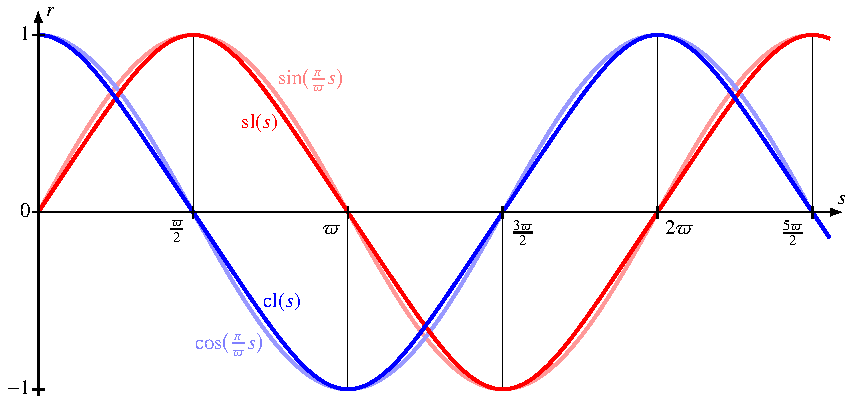
\includegraphics{chapters/110-elliptisch/images/slcl.pdf}
\caption{
Lemniskatischer Sinus und Kosinus sowie Sinus und Kosinus
mit derart skaliertem Argument, dass die Funktionen die gleichen Nullstellen
haben.
\label{buch:elliptisch:figure:slcl}}
\end{figure}


%\section*{Übungsaufgaben}
%\rhead{Übungsaufgaben}
%\aufgabetoplevel{chapters/020-exponential/uebungsaufgaben}
%\begin{uebungsaufgaben}
%\uebungsaufgabe{0}
%\uebungsaufgabe{1}
%\end{uebungsaufgaben}


%
% chapter.tex -- Beschreibung des Inhaltes
%
% (c) 2021 Prof Dr Andreas Müller, Hochschule Rapperswil
%
% !TeX spellcheck = de_CH
\chapter{Elliptische Funktionen
\label{buch:chapter:geometrie}}
\lhead{Elliptische Funktionen}
\rhead{}

Der Versuch, die Länge eines Ellipsenbogens zu berechnen, hat
in Abschnitt~\ref{buch:geometrie:subsection:hyperbeln-und-ellipsen}
zu Integralen geführt, die nicht in geschlossener Form ausgewertet
werden können.
Neben den dort gefundenen Integralen sind noch weitere, ähnlich
aufgebaute Integrale in dieser Familie zu finden.

%
% ellintegral.tex
%
% (c) 2021 Prof Dr Andreas Müller, OST Ostschweizer Fachhochschule
%
\section{Elliptische Integrale
\label{buch:elliptisch:section:integral}}
\rhead{Elliptisches Integral}
Bei der Berechnung des Ellipsenbogens in 
Abschnitt~\ref{buch:geometrie:subsection:hyperbeln-und-ellipsen}
sind wir auf ein Integral gestossen, welches sich nicht in geschlossener
Form ausdrücken liess.
Um solche Integrale in den Griff zu bekommen, ist es nötig, sie als
neue spezielle Funktionen zu definieren.

\subsection{Definition
\label{buch:elliptisch:subsection:definition}}
Ein {\em elliptisches Integral} ist ein Integral der Form
\index{elliptishes Integral}%
\index{Integral, elliptisch}%
\begin{equation}
\int R\left( x, \sqrt{p(x)}\right)\,dx
\label{buch:elliptisch:def:allgemein}
\end{equation}
wobei $R(x,y)$ eine rationale Funktion von zwei Variablen ist und
$p(x)$ ein Polynom dritten oder vierten Grades.
Hätte $p(x)$ ein mehrfache Nullstelle $x_0$, müsste es durch $(x-x_0)^2$
teilbar sein, man könnte also einen Faktor $(x-x_0)$ aus der
Wurzel im Integraneden von \eqref{buch:elliptisch:def:allgemein}
ausklammern und damit das Integral in eine Form bringen, wo $p(x)$
höchstens zweiten Grades ist.
Solche Integrale lassen sich meistens mit trigonometrischen Substitutionen
berechnen.
Wir verlangen daher, dass $p(x)$ keine mehrfachen Nullstellen hat.

Man kann zeigen, dass sich elliptische Integrale in Summen von
elementaren Funktionen und speziellen elliptischen Integralen 
der folgenden Form überführen lassen
\cite[Abschnitt 164, p.~506]{buch:smirnov32}.

\begin{definition}
\label{buch:elliptisch:def:integrale123}
Die elliptischen Integrale erster, zweiter und dritter Art sind die
Integrale
\[
\begin{aligned}
\text{1.~Art:}&&&
\int \frac{dx}{\sqrt{(1-x^2)(1-k^2x^2)}}
\\
\text{2.~Art:}&&&
\int \sqrt{\frac{1-k^2x^2}{1-x^2}}\,dx
\\
\text{3.~Art:}&&&
\int \frac{dx}{(1-nx^2)\sqrt{(1-x^2)(1-k^2x^2)}}
\end{aligned}
\]
mit $0<k<1$.
Es ist auch üblich, den Parameter $m=k^2$ zu verwenden.
\end{definition}

Wie gesagt lassen sich für diese unbestimmten Integrale keine 
geschlossenen Formen finden.
Es bleibt uns daher nichts anderes übrig, als die Integralgrenzen
festzulegen und damit eine Stammfunktion auszuwählen.

%
% Elliptisches Integral
%
\subsection{Vollständige elliptische Integrale
\label{buch:elliptisch:subsection:vollstaendig}}
In diesem Abschnitt legen wir beide Integrationsgrenzen fest und
untersuchen die entstehenenden Funktionen von den Parametern
$k$ und $n$.

\subsubsection{Definition der vollständigen elliptischen Integrale}
Da der Nenner in allen drei elliptischen Integralen eine Nullstelle
bei $\pm1$ hat, kann das Integral nur von $0$ bis $1$ erstreckt werden.

\begin{definition}
\label{buch:elliptisch:def:vollstintegrale123}
Die vollständigen elliptischen Integrale erster, zweiter und dritter
Art sind
\[
\begin{aligned}
\text{1.~Art:}&&
K(k)&=\int_0^1 \frac{dt}{\sqrt{(1-t^2)(1-k^2t^2)}} \\
\text{2.~Art:}&&
E(k)&=\int_0^1 \sqrt{\frac{1-k^2t^2}{1-t^2}}\,dt \\
\text{3.~Art:}&&
\Pi(n, k)&=\int_0^1\frac{dt}{(1-nt^2)\sqrt{(1-t^2)(1-k^2t^2)}} 
\end{aligned}
\]
mit $0<k<1$.
\end{definition}

Die Funktionen hängen stetig von $k$ ab.
Die Nullstellen des Faktors $1-k^2x^2$ liegen ausserhalb des
Integrationsintervalls und spielen daher keine Rolle.
Die Werte von $K(k)$ und $E(k)$ für $k=0$ können direkt berechnet
werden:
\begin{align*}
K(0)
=
E(0)
&=
\int_0^1 \frac{dt}{\sqrt{1-t^2}}=\frac{\pi}2.
\end{align*}
Das Integral $\Pi(n,0)$ ist etwas komplizierter.

Für $k\to 1$ ist $E(k)=1$, die Integrale $K(1)$ und $\Pi(n,1)$
sind dagegen divergent.

\subsubsection{Jacobi- und Legendre-Normalform}
Die Integrationsvariable $t$ der vollständigen elliptischen Integrale
kann durch die Substitution $t=\sin\varphi$ durch die Variable
$\varphi$ und das Integral über das Intervall $[0,1]$ durch ein
Integral über das Intervall $[0,\frac{\pi}2]$ ersetzt werden.
Mit
\[
\frac{dt}{d\varphi} = \cos\varphi = \sqrt{1-\sin^2\varphi}
\]
können die Funktionen $K(k)$, $E(k)$ und $\Pi(n,k)$ auch als
\begin{align*}
K(k)
&=
\int_0^{\frac{\pi}2}
\frac{
\sqrt{1-\sin^2\varphi}\,d\varphi
}{
\sqrt{(1-\sin^2\varphi)(1-k^2\sin^2\varphi)}
}
=
\int_0^{\frac{\pi}2}
\frac{d\varphi}{\sqrt{1-k^2\sin^2\varphi}}
\\
E(k)
&=
\int_0^{\frac{\pi}2}
\sqrt{\frac{1-k^2\sin^2\varphi}{1-\sin^2\varphi}}\sqrt{1-\sin^2\varphi}\,d\varphi
=
\int_0^{\frac{\pi}2}
\sqrt{1-k^2\sin^2\varphi}\,d\varphi
\\
\Pi(n,k)
&=
\int_0^{\frac{\pi}2}
\frac{
\sqrt{1-\sin^2\varphi}\,d\varphi
}{
(1-n\sin^2\varphi)\sqrt{(1-\sin^2\varphi)(1-k^2\sin^2\varphi)}
}
=
\int_0^{\frac{\pi}2}
\frac{
d\varphi
}{
(1-n\sin^2\varphi)\sqrt{1-k^2\sin^2\varphi}
}
\end{align*}
Diese Form wird auch die {\em Legendre-Normalform} der vollständigen 
\index{Legendre-Normalform}%
elliptischen Integrale genannt, während die Form von
Definition~\ref{buch:elliptisch:def:vollstintegrale123}
die {\em Jacobi-Normalform} heisst.
\index{Jacobi-Normalform}%

\subsubsection{Umfang einer Ellipse}
\begin{figure}
\centering
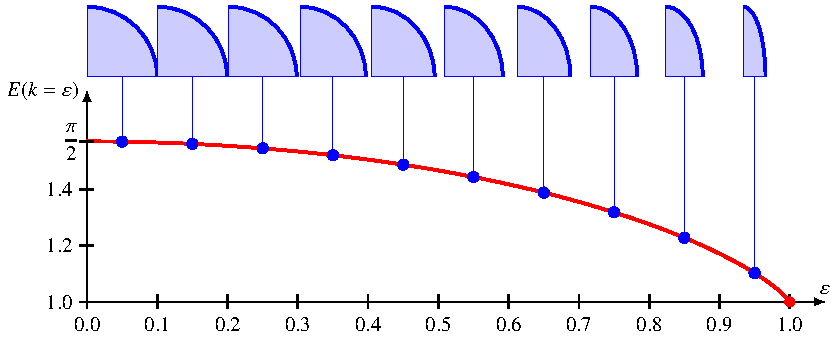
\includegraphics{chapters/110-elliptisch/images/ellipsenumfang.pdf}
\caption{Bogenlänge eines Viertels einer Ellipse mit Exzentrizität
$\varepsilon$.
\label{buch:elliptisch:fig:ellipsenumfang}}
\end{figure}
Wir zeigen, wie sich die Berechnung des Umfangs $U$ einer Ellipse
mit Halbachsen $a$ und $b$, $a\le b$, auf ein volltändiges elliptisches
Integral zurückführen lässt.
Der Fall $a>b$ kann behandelt werden, indem die $x$- und $y$-Koordinaten
vertauscht werden.

Die Parametrisierung
\[
t\mapsto \begin{pmatrix}a\cos t\\ b\sin t\end{pmatrix}
\]
einer Ellipse führt auf das Integral
\begin{align*}
U
&=
\int_0^{2\pi} \sqrt{a^2\sin^2t + b^2\cos^2 t}\,dt
\notag
\\
&=
4\int_0^{\frac{\pi}2}
\sqrt{a^2\sin^2t + b^2(1-\sin^2 t)}
\,dt
\notag
\\
&=
4b \int_0^{\frac{\pi}2} \sqrt{1-(b^2-a^2)/b^2\cdot \sin^2t}\,dt
\label{buch:elliptisch:eqn:umfangellipse}
\end{align*}
für den Umfang der Ellipse.
Bei einem Kreis ist $a=b$ und der zweite Term unter der Wurzel fällt weg,
der Umfang wird $4b\frac{\pi}2=2\pi b$.
Die Differenz $e^2=b^2-a^2$ ist die {\em lineare Exzentrizität} der Ellipse,
\index{lineare Exzentrizität}%
der Quotient $e/b$ wird die {\em numerische Exzentrizität} der Ellipse
genannt.
Insbesondere ist $k = \varepsilon$.

Das Integral~\eqref{buch:elliptisch:eqn:umfangellipse} erhält jetzt die
Form
\[
U
=
4b\int_0^{\frac{\pi}2} \sqrt{1-k^2\sin^2t}\,dt
\]
und ist damit als elliptisches Integral zweiter Art erkannt.
Für den Umfang der Ellipse finden wir damit die Formel
\[
U
=
4b E(k)
=
4b E(\varepsilon).
\]
Das vollständige elliptische Integral zweiter Art $E(\varepsilon)$
liefert also genau den Umfang der eines Viertels Ellipse mit
numerischer Exzentrizität $\varepsilon$ und kleiner Halbachse $1$.

\subsubsection{Komplementäre Integrale}
XXX Komplementäre Integrale \\

\subsubsection{Ableitung}
XXX Ableitung \\
XXX Stammfunktion \\

\subsection{Unvollständige elliptische Integrale}
XXX Vollständige und Unvollständige Integrale \\
XXX Additionstheoreme \\
XXX Parameterkonventionen \\

\subsection{Potenzreihe}
XXX Potenzreihen \\
XXX Als hypergeometrische Funktionen \\



\section{Jacobische elliptische Funktionen}

Für das elliptische Filter werden, wie es der Name bereits deutet, elliptische Funktionen gebraucht.
Wie die trigonometrischen Funktionen Zusammenhänge eines Kreises darlegen, beschreiben die elliptischen Funktionen Ellipsen.
Es ist daher naheliegend, dass der Kosinus des Tschebyscheff-Filters gegen ein elliptisches Pendant ausgetauscht werden könnte.
Der Begriff elliptische Funktion wird für sehr viele Funktionen gebraucht, daher ist es hier wichtig zu erwähnen, dass es ausschliesslich um die Jacobischen elliptischen Funktionen geht.

\subsection{Grundlegende Eigenschaften}

Die Jacobi elliptischen Funktionen werden ausführlich im Kapitel \ref{buch:elliptisch:section:jacobi} behandelt.
Im Wesentlichen erweitern die Jacobi elliptischen Funktionen die trigonometrische Funktionen für Ellipsen.
Zum Beispiel gibt es analog zum Sinus den elliptischen $\sn(z, k)$.
Im Gegensatz zum den trigonometrischen Funktionen haben die elliptischen Funktionen zwei Parameter.
Den \textit{elliptische Modul} $k$, der die Exzentrizität der Ellipse parametrisiert und das Winkelargument $z$.
Im Kreis ist der Radius für alle Winkel konstant, bei Ellipsen ändert sich das.
Dies hat zur Folge, dass bei einer Ellipse die Kreisbogenlänge nicht linear zum Winkel verläuft.
Darum kann hier nicht der gewohnte Winkel verwendet werden.
Das Winkelargument $z$ kann durch das elliptische Integral erster Art
\begin{equation}
    z
    =
    F(\phi, k)
    =
    \int_{0}^{\phi}
    \frac{
        d\theta
    }{
        \sqrt{
            1-k^2 \sin^2 \theta
        }
    }
\end{equation}
mit dem Winkel $\phi$ in Verbindung gebracht werden.

Dabei wird das vollständige und unvollständige elliptische integral unterschieden.
Beim vollständigen Integral
\begin{equation}
    K(k)
    =
    \int_{0}^{\pi / 2}
    \frac{
        d\theta
    }{
        \sqrt{
            1-k^2 \sin^2 \theta
        }
    }
\end{equation}
wird über ein viertel Ellipsenbogen integriert, also bis $\phi=\pi/2$ und liefert das Winkelargument für eine Vierteldrehung.
Die Zahl wird oft auch abgekürzt mit $K = K(k)$ und ist für das elliptische Filter sehr relevant.
Alle elliptischen Funktionen sind somit $4K$-periodisch.

Neben dem $\sn$ gibt es zwei weitere elliptische Basisfunktionen $\cn$ und $\dn$.
Dazu kommen noch weitere abgeleitete Funktionen, die durch Quotienten und Kehrwerte dieser Funktionen zustande kommen.
Insgesamt sind es die zwölf Funktionen
\begin{equation*}
    \sn \quad
    \ns \quad
    \scelliptic \quad
    \sd \quad
    \cn \quad
    \nc \quad
    \cs \quad
    \cd \quad
    \dn \quad
    \nd \quad
    \ds \quad
    \dc.
\end{equation*}

Die Jacobischen elliptischen Funktionen können mit der inversen Funktion des vollständigen elliptischen Integrals erster Art
\begin{equation}
    \phi = F^{-1}(z, k)
\end{equation}
definiert werden. Dabei ist zu beachten dass nur das $z$ Argument der Funktion invertiert wird, also
\begin{equation}
    z = F(\phi, k)
    \Leftrightarrow
    \phi = F^{-1}(z, k).
\end{equation}
Mithilfe von $F^{-1}$ kann zum Beispiel $sn^{-1}$ mit dem elliptischen Integral dargestellt werden:
\begin{equation}
    \sin(\phi)
    =
    \sin \left( F^{-1}(z, k) \right)
    =
    \sn(z, k)
    =
    w.
\end{equation}

% \begin{equation} %TODO remove unnecessary equations
%     \phi
%     =
%      F^{-1}(z, k)
%      =
%      \sin^{-1} \big( \sn (z, k ) \big)
%      =
%     \sin^{-1} ( w )
% \end{equation}

% \begin{equation}
%     F(\phi, k)
%     =
%     z
%     =
%     F( \sin^{-1} \big( \sn (z, k ) \big) , k)
%     =
%     F( \sin^{-1} ( w ), k)
% \end{equation}

% \begin{equation}
%     \sn^{-1}(w, k)
%     =
%     F(\phi, k),
%     \quad
%     \phi = \sin^{-1}(w)
% \end{equation}

\subsection{Die Funktion $\sn^{-1}$}

Beim Tschebyscheff-Filter konnten wir mit Betrachten des Arcuscosinus die Funktionalität erklären.
Für das Elliptische Filter machen wir die gleiche Betrachtung mit der $\sn^{-1}$-Funktion.
Der $\sn^{-1}$ ist durch das elliptische Integral
\begin{align}
    \sn^{-1}(w, k)
        & =
    \int_{0}^{\phi}
    \frac{
        d\theta
    }{
        \sqrt{
            1-k^2 \sin^2 \theta
        }
    },
    \quad
    \phi = \sin^{-1}(w)
    \\
        & =
    \int_{0}^{w}
    \frac{
        dt
    }{
        \sqrt{
            (1-t^2)(1-k^2 t^2)
        }
    }
\end{align}
beschrieben.
Dazu betrachten wir wieder den Integranden
\begin{equation}
    \frac{
        1
    }{
        \sqrt{
            (1-t^2)(1-k^2 t^2)
        }
    }.
\end{equation}
Beim $\cos^{-1}(x)$ haben wir gesehen, dass die analytische Fortsetzung bei $x < -1$ und $x > 1$ rechtwinklig in die komplexen Zahlen wandert.
Wenn man das Gleiche mit $\sn^{-1}(w, k)$ macht, erkennt man zwei interessante Stellen.
Die erste ist die gleiche wie beim $\cos^{-1}(x)$ nämlich bei $t = \pm 1$.
Der erste Term unter der Wurzel wird dann negativ, während der zweite noch positiv ist, da $k \leq 1$.
Ab diesem Punkt knickt die Funktion in die imaginäre Richtung ab.
Bei $t = 1/k$ ist auch der zweite Term negativ und die Funktion verläuft in die negative reelle Richtung.
Abbildung \ref{ellfilter:fig:sn} zeigt den Verlauf der Funktion in der komplexen Ebene.
\begin{figure}
    \centering
    \begin{tikzpicture}[>=stealth', auto, node distance=2cm, scale=1.2]

    \tikzstyle{zero} = [draw, circle, inner sep =0, minimum height=0.15cm]

    \tikzset{pole/.style={cross out, draw=black, minimum size=(0.15cm-\pgflinewidth), inner sep=0pt, outer sep=0pt}}

    \begin{scope}[xscale=0.9, yscale=1.8]

        \draw[gray, ->] (0,-1.5) -- (0,1.5) node[anchor=south]{$\mathrm{Im}~z$};
        \draw[gray, ->] (-5,0) -- (5,0) node[anchor=west]{$\mathrm{Re}~z$};

        \begin{scope}

            \clip(-4.5,-1.25) rectangle (4.5,1.25);

            \fill[yellow!30] (0,0) rectangle (1, 0.5);

            \begin{scope}[xshift=-1cm]

                \foreach \i in {-2,...,2} {
                    \foreach \j in {-2,...,1} {
                        \begin{scope}[xshift=\i*4cm, yshift=\j*1cm]
                            \draw[<-, blue!50] (0, 0) -- (0,0.5);
                            \draw[<-, cyan!50] (1, 0) -- (0,0);
                            \draw[<-, darkgreen!50] (2, 0) -- (1,0);
                            \draw[<-, orange!50] (2,0.5) -- (2, 0);
                            \draw[<-, red!50] (1, 0.5) -- (2,0.5);
                            \draw[<-, purple!50] (0, 0.5) -- (1,0.5);
                            \draw[<-, blue!50] (0,1) -- (0,0.5);
                            \draw[<-, orange!50] (2,0.5) -- (2, 1);
                            \draw[<-, red!50] (3, 0.5) -- (2,0.5);
                            \draw[<-, purple!50] (4, 0.5) -- (3,0.5);
                            \draw[<-, darkgreen!50] (2, 0) -- (3,0);
                            \draw[<-, cyan!50] (3, 0) -- (4,0);
                        \end{scope}
                    }
                }

                % \pause
                \draw[ultra thick, <-, darkgreen] (2, 0) -- (1,0);
                % \pause
                \draw[ultra thick, <-, orange] (2,0.5) -- (2, 0);
                % \pause
                \draw[ultra thick, <-, red] (1, 0.5) -- (2,0.5);
                % \pause
                \draw[ultra thick, <-, blue] (0, 0) -- (0,0.5);
                \draw[ultra thick, <-, purple] (0, 0.5) -- (1,0.5);
                \draw[ultra thick, <-, cyan] (1, 0) -- (0,0);
                % \pause


                \foreach \i in {-2,...,2} {
                    \foreach \j in {-2,...,1} {
                        \begin{scope}[xshift=\i*4cm, yshift=\j*1cm]
                            \node[zero] at ( 1, 0) {};
                            \node[zero] at ( 3, 0) {};
                            \node[pole] at ( 1,0.5) {};
                            \node[pole] at ( 3,0.5) {};
                        \end{scope}
                    }
                }

            \end{scope}

        \end{scope}

        \draw[gray] ( 1,0) +(0,0.1) -- +(0, -0.1) node[inner sep=0, anchor=north] {\small $K$};
        \draw[gray]  (0, 0.5) +(0.1, 0) -- +(-0.1, 0) node[inner sep=0, anchor=east]{\small $jK^\prime$};

    \end{scope}

    \node[zero] at (4,3) (n) {};
    \node[anchor=west] at (n.east) {Zero};
    \node[pole, below=0.25cm of n] (n) {};
    \node[anchor=west] at (n.east) {Pole};

    \begin{scope}[yshift=-4cm, xscale=0.75]

        \draw[gray, ->] (-6,0) -- (6,0) node[anchor=west]{$w$};

        \draw[ultra thick, ->, purple] (-5, 0) -- (-3, 0);
        \draw[ultra thick, ->, blue]      (-3, 0) -- (-2, 0);
        \draw[ultra thick, ->, cyan]       (-2, 0) -- (0, 0);
        \draw[ultra thick, ->, darkgreen]    (0, 0) -- (2, 0);
        \draw[ultra thick, ->, orange] (2, 0) -- (3, 0);
        \draw[ultra thick, ->, red] (3, 0) -- (5, 0);

        \node[anchor=south] at (-5,0) {$-\infty$};
        \node[anchor=south] at (-3,0) {$-1/k$};
        \node[anchor=south] at (-2,0) {$-1$};
        \node[anchor=south] at (0,0) {$0$};
        \node[anchor=south] at (2,0) {$1$};
        \node[anchor=south] at (3,0) {$1/k$};
        \node[anchor=south] at (5,0) {$\infty$};

    \end{scope}


\end{tikzpicture}
    \caption{
        $z$-Ebene der Funktion $z = \sn^{-1}(w, k)$.
        Die Funktion ist in der realen Achse $4K$-periodisch und in der imaginären Achse $2jK^\prime$-periodisch.
    }
    \label{ellfilter:fig:sn}
\end{figure}
In der reellen Richtung ist sie $4K(k)$-periodisch und in der imaginären Richtung $4K^\prime(k)$-periodisch, wobei $K^\prime$ das komplementäre vollständige Elliptische Integral ist:
\begin{equation}
    K^\prime(k)
    =
    \int_{0}^{\pi / 2}
    \frac{
        d\theta
    }{
        \sqrt{
            1-{k^\prime}^2 \sin^2 \theta
        }
    },
    \quad
    k^\prime = \sqrt{1-k^2}.
\end{equation}

%
% lemniskate.tex
%
% (c) 2021 Prof Dr Andreas Müller, OST Ostschweizer Fachhochschule
%
\section{Lemniskatischer Sinus
\label{buch:elliptisch:section:lemniskate}}
\rhead{Lemniskatischer Sinus}
Historisch war der {\em lemniskatische Sinus} die erste ellptische
Funktion, die Gauss bereits als 19-jähriger untersucht, aber nicht 
veröffentlich hat.
In diesem Abschnitt soll die Verbindung zu den Jacobischen
elliptischen Funktionen hergestellt werden.

\subsection{Lemniskate
\label{buch:gemotrie:subsection:lemniskate}}
\begin{figure}
\centering
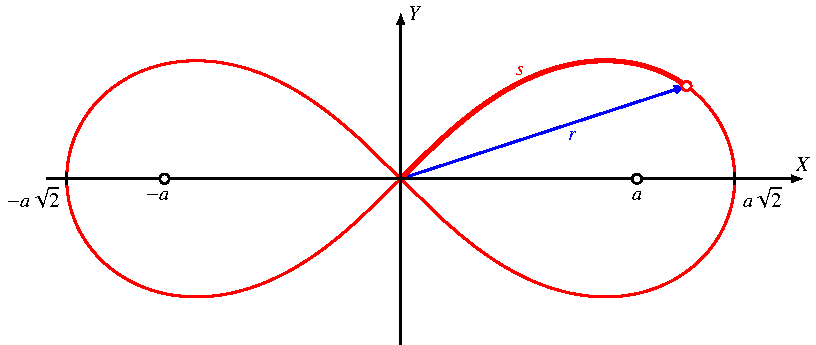
\includegraphics{chapters/110-elliptisch/images/lemniskate.pdf}
\caption{Bogenlänge und Radius der Lemniskate von Bernoulli.
\label{buch:elliptisch:fig:lemniskate}}
\end{figure}
Die Lemniskate von Bernoulli ist die Kurve vierten Grades mit der Gleichung
\begin{equation}
(X^2+Y^2)^2 = 2a^2(X^2-Y^2).
\label{buch:elliptisch:eqn:lemniskate}
\end{equation}
Sie ist in Abbildung~\ref{buch:elliptisch:fig:lemniskate}
dargestellt.
Die beiden Scheitel der Lemniskate befinden sich bei $X_s=\pm a\sqrt{2}$.
Dividiert man die Gleichung der Lemniskate durch $X_s^2=4a^4$ entsteht 
\begin{equation}
\biggl(
\biggl(\frac{X}{a\sqrt{2}}\biggr)^2
+
\biggl(\frac{Y}{a\sqrt{2}}\biggr)^2
\biggr)^2
=
2\frac{a^2}{2a^2}\biggl(
\biggl(\frac{X}{a\sqrt{2}}\biggr)^2
-
\biggl(\frac{Y}{a\sqrt{2}}\biggr)^2
\biggr).
\qquad
\Leftrightarrow
\qquad
(x^2+y^2)^2 = x^2-y^2,
\label{buch:elliptisch:eqn:lemniskatenormiert}
\end{equation}
wobei wir $x=X/a\sqrt{2}$ und $y=Y/a\sqrt{2}$ gesetzt haben.
In dieser Normierung liegen die Scheitel bei $\pm 1$.
Dies ist die Skalierung, die für die Definition des lemniskatischen
Sinus und Kosinus verwendet werden soll.

In Polarkoordinaten $x=r\cos\varphi$ und $y=r\sin\varphi$
gilt nach Einsetzen in \eqref{buch:elliptisch:eqn:lemniskatenormiert}
\begin{equation}
r^4
=
r^2(\cos^2\varphi-\sin^2\varphi)
=
r^2\cos2\varphi
\qquad\Rightarrow\qquad
r^2 = \cos 2\varphi
\label{buch:elliptisch:eqn:lemniskatepolar}
\end{equation}
als Darstellung der Lemniskate in Polardarstellung.
Sie gilt für Winkel $\varphi\in[-\frac{\pi}4,\frac{\pi}4]$ für das
rechte Blatt und $\varphi\in[\frac{3\pi}4,\frac{5\pi}4]$ für das linke
Blatt der Lemniskate.

\subsection{Bogenlänge}
Die Funktionen
\begin{equation}
x(r) = \frac{r}{\sqrt{2}}\sqrt{1+r^2},
\quad
y(r) = \frac{r}{\sqrt{2}}\sqrt{1-r^2}
\label{buch:geometrie:eqn:lemniskateparam}
\end{equation}
erfüllen
\begin{align*}
x(r)^2-y(r)^2
&=
\frac{r^2(1+r^2)}{2}-\frac{r^2(1-r^2)}{2}
\\
&
=
r^4
=
(x(r)^2 + y(r)^2)^2,
\end{align*}
sie stellen also eine Parametrisierung der Lemniskate dar.

Mit Hilfe der Parametrisierung~\eqref{buch:geometrie:eqn:lemniskateparam}
kann man die Länge $s$ des in Abbildung~\ref{buch:elliptisch:fig:lemniskate}
dargestellten Bogens der Lemniskate berechnen.
Dazu benötigt man die Ableitungen nach $r$, die man mit der Produkt- und
Kettenregel berechnen kann:
\begin{align*}
\dot{x}(r)
&=
\frac{\sqrt{1+r^2}}{\sqrt{2}}
+
\frac{r^2}{\sqrt{2}\sqrt{1+r^2}}
&&\Rightarrow&
\dot{x}(r)^2
&=
\frac{1+r^2}{2} +r^2 + \frac{r^4}{2(1+r^2)}
\\
\dot{y}(r)
&=
\frac{\sqrt{1-r^2}}{\sqrt{2}}
-
\frac{r^2}{\sqrt{2}\sqrt{1-r^2}}
&&\Rightarrow&
\dot{y}(r)^2
&=
\frac{1-r^2}{2} -r^2 + \frac{r^4}{2(1-r^2)}
\end{align*}
Die Summe der Quadrate ist
\begin{align*}
\dot{x}(r)^2 + \dot{y}(r)^2
&=
1 + r^4\frac{1-r^2+1+r^2}{2(1+r^2)(1-r^2)}
=
1+r^4\frac{2}{2(1-r^4)}
=
\frac{1-r^4+r^4}{1-r^4}
=
\frac1{1-r^4}.
\end{align*}
Durch Einsetzen in das Integral für die Bogenlänge bekommt man
\begin{equation}
s(r)
=
\int_0^r
\frac{1}{\sqrt{1-t^4}}\,dt.
\label{buch:elliptisch:eqn:lemniskatebogenlaenge}
\end{equation}

%
% Als elliptisches Integral
%
\subsection{Darstellung als elliptisches Integral}
Das unvollständige elliptische Integral erster Art mit Parameter
$k^2=-1$ oder $k=i$ ist
\[
K(r,i)
=
\int_0^x \frac{dt}{\sqrt{(1-t^2)(1-i^2 t^2)}}
=
\int_0^x \frac{dt}{\sqrt{(1-t^2)(1-(-1)t^2)}}
=
\int_0^x \frac{dt}{\sqrt{1-t^4}}
=
s(r).
\]
Der lemniskatische Sinus ist also eine Umkehrfunktion des
elliptischen Integrals erster Art für den speziellen Wert $i$ des
Parameters $k$.

Die Länge des rechten Blattes der Lemniskate wird mit $\varpi$ bezeichnet
und hat den numerischen Wert
\[
\varpi
=
2\int_0^1\sqrt{\frac{1}{1-t^4}}\,dt
=
2.6220575542.
\]
$\varpi$ ist auch als die {\em lemniskatische Konstante} bekannt.
\index{lemniskatische Konstante}%
Der Lemniskatenbogen zwischen dem Nullpunkt und $(1,0)$ hat die Länge
$\varpi/2$.

%
%  Bogenlängenparametrisierung
%
\subsection{Bogenlängenparametrisierung}
Die Lemniskate mit der Gleichung
\[
(X^2+X^2)^2=2(X^2-X^2)
\]
(der Fall $a=1$ in \eqref{buch:elliptisch:eqn:lemniskate})
kann mit Jacobischen elliptischen Funktionen
parametrisiert werden.
Dazu schreibt man
\[
\left.
\begin{aligned}
X(t)
&=
\sqrt{2}\operatorname{cn}(t,k) \operatorname{dn}(t,k)
\\
Y(t)
&=
\phantom{\sqrt{2}}
\operatorname{cn}(t,k) \operatorname{sn}(t,k)
\end{aligned}
\quad\right\}
\qquad\text{mit $k=\displaystyle\frac{1}{\sqrt{2}}$}
\]
und berechnet die beiden Seiten der definierenden Gleichung der
Lemniskate.
Zunächst ist
\begin{align*}
X(t)^2
&=
2\operatorname{cn}(t,k)^2
\operatorname{dn}(t,k)^2
\\
Y(t)^2
&=
\operatorname{cn}(t,k)^2
\operatorname{sn}(t,k)^2
\\
X(t)^2+Y(t)^2
&=
2\operatorname{cn}(t,k)^2
\bigl(
\underbrace{
\operatorname{dn}(t,k)^2
+{\textstyle\frac12}
\operatorname{sn}(t,k)^2
}_{\displaystyle =1}
\bigr)
%\\
%&
=
2\operatorname{cn}(t,k)^2
\\
X(t)^2-Y(t)^2
&=
\operatorname{cn}(t,k)^2
\bigl(
2\operatorname{dn}(t,k)^2 - \operatorname{sn}(t,k)^2
\bigr)
\\
&=
\operatorname{cn}(t,k)^2
\bigl(
2\bigl({\textstyle\frac12}+{\textstyle\frac12}\operatorname{cn}(t,k)^2\bigr)
-
\bigl(1-\operatorname{cn}(t,k)^2\bigr)
\bigr)
\\
&=
2\operatorname{cn}(t,k)^4
\\
\Rightarrow\qquad
(X(t)^2+Y(t)^2)^2
&=
4\operatorname{cn}(t,k)^4
=
2(X(t)^2-Y(t)^2).
\end{align*}
Wir zeigen jetzt, dass dies tatsächlich eine Bogenlängenparametrisierung
der Lemniskate ist.
Dazu berechnen wir die Ableitungen
\begin{align*}
\dot{X}(t)
&=
\sqrt{2}\operatorname{cn}'(t,k)\operatorname{dn}(t,k)
+
\sqrt{2}\operatorname{cn}(t,k)\operatorname{dn}'(t,k)
\\
&=
-\sqrt{2}\operatorname{sn}(t,k)\operatorname{dn}(t,k)^2
-\frac12\sqrt{2}\operatorname{sn}(t,k)\operatorname{cn}(t,k)^2
\\
&=
-\sqrt{2}\operatorname{sn}(t,k)\bigl(
1-{\textstyle\frac12}\operatorname{sn}(t,k)^2
+{\textstyle\frac12}-{\textstyle\frac12}\operatorname{sn}(u,t)^2
\bigr)
\\
&=
\sqrt{2}\operatorname{sn}(t,k)
\bigl(
{\textstyle \frac32}-\operatorname{sn}(t,k)^2
\bigr)
\\
\dot{X}(t)^2
&=
2\operatorname{sn}(t,k)^2
\bigl(
{\textstyle \frac32}-\operatorname{sn}(t,k)^2
\bigr)^2
\\
&=
{\textstyle\frac{9}{2}}\operatorname{sn}(t,k)^2
-
6\operatorname{sn}(t,k)^4
+2\operatorname{sn}(t,k)^6
\\
\dot{Y}(t)
&=
\operatorname{cn}'(t,k)\operatorname{sn}(t,k)
+
\operatorname{cn}(t,k)\operatorname{sn}'(t,k)
\\
&=
-\operatorname{sn}(t,k)^2
\operatorname{dn}(t,k)
+\operatorname{cn}(t,k)^2
\operatorname{dn}(t,k)
\\
&=
\operatorname{dn}(t,k)\bigl(1-2\operatorname{sn}(t,k)^2\bigr)
\\
\dot{Y}(t)^2
&=
\bigl(1-{\textstyle\frac12}\operatorname{sn}(t,k)^2\bigr)
\bigl(1-2\operatorname|{sn}(t,k)^2\bigr)^2
\\
&=
1-{\textstyle\frac{9}{2}}\operatorname{sn}(t,k)^2
+6\operatorname{sn}(t,k)^4
-2\operatorname{sn}(t,k)^6
\\
\dot{X}(t)^2 + \dot{Y}(t)^2
&=
1.
\end{align*}
Dies bedeutet, dass die Bogenlänge zwischen den Parameterwerten $0$ und $s$
\[
\int_0^s
\sqrt{\dot{X}(t)^2 + \dot{Y}(t)^2}
\,dt
=
\int_0^s\,dt
=
s,
\]
der Parameter $t$ ist also ein Bogenlängenparameter.

Die mit dem Faktor $1/\sqrt{2}$ skalierte Standard-Lemniskate mit der
Gleichung
\[
(x^2+y^2)^2 = x^2-y^2
\]
hat daher eine Bogenlängenparametrisierung mit
\begin{equation}
\begin{aligned}
x(t)
&=
\phantom{\frac{1}{\sqrt{2}}}
\operatorname{cn}(\sqrt{2}t,k)\operatorname{dn}(\sqrt{2}t,k)
\\
y(t)
&=
\frac{1}{\sqrt{2}}\operatorname{cn}(\sqrt{2}t,k)\operatorname{sn}(\sqrt{2}t,k)
\end{aligned}
\label{buch:elliptisch:lemniskate:bogenlaenge}
\end{equation}

\subsection{Der lemniskatische Sinus und Kosinus}
Der Sinus Berechnet die Gegenkathete zu einer gegebenen Bogenlänge des
Kreises, er ist die Umkehrfunktion der Funktion, die der Gegenkathete
die Bogenlänge zuordnet.

Daher ist es naheliegend, die Umkehrfunktion von $s(r)$ in 
\eqref{buch:elliptisch:eqn:lemniskatebogenlaenge}
den {\em lemniskatischen Sinus} zu nennen mit der Bezeichnung
$r=\operatorname{sl} s$.

Der Kosinus ist der Sinus des komplementären Winkels.
Auch für die lemniskatische Bogenlänge $s(r)$ lässt sich eine
komplementäre Bogenlänge definieren, nämlich die Bogenlänge zwischen
dem Punkt $(x(r), y(r))$ und $(1,0)$.

Da die Parametrisierung~\eqref{buch:elliptisch:lemniskate:bogenlaenge}
eine Bogenlängenparametrisierung ist, darf man $t=s$ schreiben.
Dann kann man aber auch $r(s)$ daraus berechnen,
es ist
\[
r(s)^2
=
x(s)^2 + y(s)^2
=
\operatorname{cn}(s\sqrt{2},k)^2
\qquad\Rightarrow\qquad
r(s)
=
\operatorname{cn}(s\sqrt{2},k)
\]

\begin{figure}
\centering
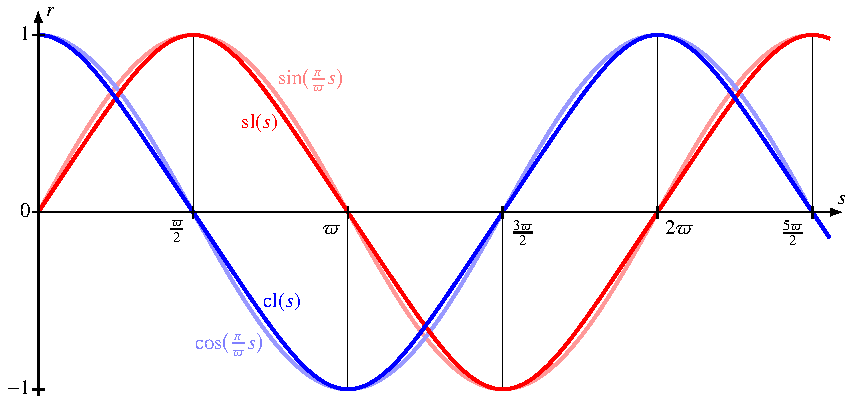
\includegraphics{chapters/110-elliptisch/images/slcl.pdf}
\caption{
Lemniskatischer Sinus und Kosinus sowie Sinus und Kosinus
mit derart skaliertem Argument, dass die Funktionen die gleichen Nullstellen
haben.
\label{buch:elliptisch:figure:slcl}}
\end{figure}


%\section*{Übungsaufgaben}
%\rhead{Übungsaufgaben}
%\aufgabetoplevel{chapters/020-exponential/uebungsaufgaben}
%\begin{uebungsaufgaben}
%\uebungsaufgabe{0}
%\uebungsaufgabe{1}
%\end{uebungsaufgaben}


%
% chapter.tex -- Beschreibung des Inhaltes
%
% (c) 2021 Prof Dr Andreas Müller, Hochschule Rapperswil
%
% !TeX spellcheck = de_CH
\chapter{Elliptische Funktionen
\label{buch:chapter:geometrie}}
\lhead{Elliptische Funktionen}
\rhead{}

Der Versuch, die Länge eines Ellipsenbogens zu berechnen, hat
in Abschnitt~\ref{buch:geometrie:subsection:hyperbeln-und-ellipsen}
zu Integralen geführt, die nicht in geschlossener Form ausgewertet
werden können.
Neben den dort gefundenen Integralen sind noch weitere, ähnlich
aufgebaute Integrale in dieser Familie zu finden.

%
% ellintegral.tex
%
% (c) 2021 Prof Dr Andreas Müller, OST Ostschweizer Fachhochschule
%
\section{Elliptische Integrale
\label{buch:elliptisch:section:integral}}
\rhead{Elliptisches Integral}
Bei der Berechnung des Ellipsenbogens in 
Abschnitt~\ref{buch:geometrie:subsection:hyperbeln-und-ellipsen}
sind wir auf ein Integral gestossen, welches sich nicht in geschlossener
Form ausdrücken liess.
Um solche Integrale in den Griff zu bekommen, ist es nötig, sie als
neue spezielle Funktionen zu definieren.

\subsection{Definition
\label{buch:elliptisch:subsection:definition}}
Ein {\em elliptisches Integral} ist ein Integral der Form
\index{elliptishes Integral}%
\index{Integral, elliptisch}%
\begin{equation}
\int R\left( x, \sqrt{p(x)}\right)\,dx
\label{buch:elliptisch:def:allgemein}
\end{equation}
wobei $R(x,y)$ eine rationale Funktion von zwei Variablen ist und
$p(x)$ ein Polynom dritten oder vierten Grades.
Hätte $p(x)$ ein mehrfache Nullstelle $x_0$, müsste es durch $(x-x_0)^2$
teilbar sein, man könnte also einen Faktor $(x-x_0)$ aus der
Wurzel im Integraneden von \eqref{buch:elliptisch:def:allgemein}
ausklammern und damit das Integral in eine Form bringen, wo $p(x)$
höchstens zweiten Grades ist.
Solche Integrale lassen sich meistens mit trigonometrischen Substitutionen
berechnen.
Wir verlangen daher, dass $p(x)$ keine mehrfachen Nullstellen hat.

Man kann zeigen, dass sich elliptische Integrale in Summen von
elementaren Funktionen und speziellen elliptischen Integralen 
der folgenden Form überführen lassen
\cite[Abschnitt 164, p.~506]{buch:smirnov32}.

\begin{definition}
\label{buch:elliptisch:def:integrale123}
Die elliptischen Integrale erster, zweiter und dritter Art sind die
Integrale
\[
\begin{aligned}
\text{1.~Art:}&&&
\int \frac{dx}{\sqrt{(1-x^2)(1-k^2x^2)}}
\\
\text{2.~Art:}&&&
\int \sqrt{\frac{1-k^2x^2}{1-x^2}}\,dx
\\
\text{3.~Art:}&&&
\int \frac{dx}{(1-nx^2)\sqrt{(1-x^2)(1-k^2x^2)}}
\end{aligned}
\]
mit $0<k<1$.
Es ist auch üblich, den Parameter $m=k^2$ zu verwenden.
\end{definition}

Wie gesagt lassen sich für diese unbestimmten Integrale keine 
geschlossenen Formen finden.
Es bleibt uns daher nichts anderes übrig, als die Integralgrenzen
festzulegen und damit eine Stammfunktion auszuwählen.

%
% Elliptisches Integral
%
\subsection{Vollständige elliptische Integrale
\label{buch:elliptisch:subsection:vollstaendig}}
In diesem Abschnitt legen wir beide Integrationsgrenzen fest und
untersuchen die entstehenenden Funktionen von den Parametern
$k$ und $n$.

\subsubsection{Definition der vollständigen elliptischen Integrale}
Da der Nenner in allen drei elliptischen Integralen eine Nullstelle
bei $\pm1$ hat, kann das Integral nur von $0$ bis $1$ erstreckt werden.

\begin{definition}
\label{buch:elliptisch:def:vollstintegrale123}
Die vollständigen elliptischen Integrale erster, zweiter und dritter
Art sind
\[
\begin{aligned}
\text{1.~Art:}&&
K(k)&=\int_0^1 \frac{dt}{\sqrt{(1-t^2)(1-k^2t^2)}} \\
\text{2.~Art:}&&
E(k)&=\int_0^1 \sqrt{\frac{1-k^2t^2}{1-t^2}}\,dt \\
\text{3.~Art:}&&
\Pi(n, k)&=\int_0^1\frac{dt}{(1-nt^2)\sqrt{(1-t^2)(1-k^2t^2)}} 
\end{aligned}
\]
mit $0<k<1$.
\end{definition}

Die Funktionen hängen stetig von $k$ ab.
Die Nullstellen des Faktors $1-k^2x^2$ liegen ausserhalb des
Integrationsintervalls und spielen daher keine Rolle.
Die Werte von $K(k)$ und $E(k)$ für $k=0$ können direkt berechnet
werden:
\begin{align*}
K(0)
=
E(0)
&=
\int_0^1 \frac{dt}{\sqrt{1-t^2}}=\frac{\pi}2.
\end{align*}
Das Integral $\Pi(n,0)$ ist etwas komplizierter.

Für $k\to 1$ ist $E(k)=1$, die Integrale $K(1)$ und $\Pi(n,1)$
sind dagegen divergent.

\subsubsection{Jacobi- und Legendre-Normalform}
Die Integrationsvariable $t$ der vollständigen elliptischen Integrale
kann durch die Substitution $t=\sin\varphi$ durch die Variable
$\varphi$ und das Integral über das Intervall $[0,1]$ durch ein
Integral über das Intervall $[0,\frac{\pi}2]$ ersetzt werden.
Mit
\[
\frac{dt}{d\varphi} = \cos\varphi = \sqrt{1-\sin^2\varphi}
\]
können die Funktionen $K(k)$, $E(k)$ und $\Pi(n,k)$ auch als
\begin{align*}
K(k)
&=
\int_0^{\frac{\pi}2}
\frac{
\sqrt{1-\sin^2\varphi}\,d\varphi
}{
\sqrt{(1-\sin^2\varphi)(1-k^2\sin^2\varphi)}
}
=
\int_0^{\frac{\pi}2}
\frac{d\varphi}{\sqrt{1-k^2\sin^2\varphi}}
\\
E(k)
&=
\int_0^{\frac{\pi}2}
\sqrt{\frac{1-k^2\sin^2\varphi}{1-\sin^2\varphi}}\sqrt{1-\sin^2\varphi}\,d\varphi
=
\int_0^{\frac{\pi}2}
\sqrt{1-k^2\sin^2\varphi}\,d\varphi
\\
\Pi(n,k)
&=
\int_0^{\frac{\pi}2}
\frac{
\sqrt{1-\sin^2\varphi}\,d\varphi
}{
(1-n\sin^2\varphi)\sqrt{(1-\sin^2\varphi)(1-k^2\sin^2\varphi)}
}
=
\int_0^{\frac{\pi}2}
\frac{
d\varphi
}{
(1-n\sin^2\varphi)\sqrt{1-k^2\sin^2\varphi}
}
\end{align*}
Diese Form wird auch die {\em Legendre-Normalform} der vollständigen 
\index{Legendre-Normalform}%
elliptischen Integrale genannt, während die Form von
Definition~\ref{buch:elliptisch:def:vollstintegrale123}
die {\em Jacobi-Normalform} heisst.
\index{Jacobi-Normalform}%

\subsubsection{Umfang einer Ellipse}
\begin{figure}
\centering
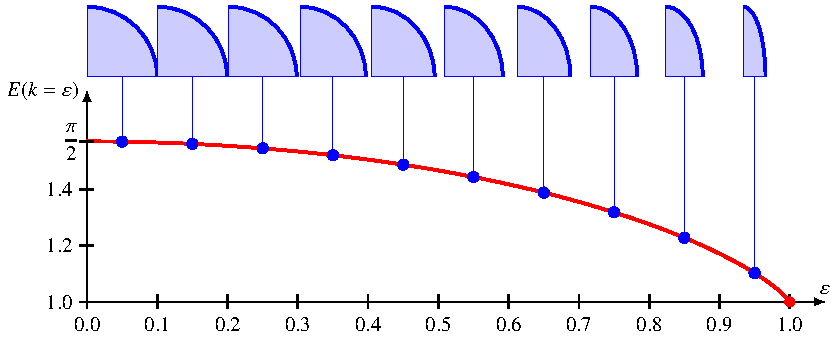
\includegraphics{chapters/110-elliptisch/images/ellipsenumfang.pdf}
\caption{Bogenlänge eines Viertels einer Ellipse mit Exzentrizität
$\varepsilon$.
\label{buch:elliptisch:fig:ellipsenumfang}}
\end{figure}
Wir zeigen, wie sich die Berechnung des Umfangs $U$ einer Ellipse
mit Halbachsen $a$ und $b$, $a\le b$, auf ein volltändiges elliptisches
Integral zurückführen lässt.
Der Fall $a>b$ kann behandelt werden, indem die $x$- und $y$-Koordinaten
vertauscht werden.

Die Parametrisierung
\[
t\mapsto \begin{pmatrix}a\cos t\\ b\sin t\end{pmatrix}
\]
einer Ellipse führt auf das Integral
\begin{align*}
U
&=
\int_0^{2\pi} \sqrt{a^2\sin^2t + b^2\cos^2 t}\,dt
\notag
\\
&=
4\int_0^{\frac{\pi}2}
\sqrt{a^2\sin^2t + b^2(1-\sin^2 t)}
\,dt
\notag
\\
&=
4b \int_0^{\frac{\pi}2} \sqrt{1-(b^2-a^2)/b^2\cdot \sin^2t}\,dt
\label{buch:elliptisch:eqn:umfangellipse}
\end{align*}
für den Umfang der Ellipse.
Bei einem Kreis ist $a=b$ und der zweite Term unter der Wurzel fällt weg,
der Umfang wird $4b\frac{\pi}2=2\pi b$.
Die Differenz $e^2=b^2-a^2$ ist die {\em lineare Exzentrizität} der Ellipse,
\index{lineare Exzentrizität}%
der Quotient $e/b$ wird die {\em numerische Exzentrizität} der Ellipse
genannt.
Insbesondere ist $k = \varepsilon$.

Das Integral~\eqref{buch:elliptisch:eqn:umfangellipse} erhält jetzt die
Form
\[
U
=
4b\int_0^{\frac{\pi}2} \sqrt{1-k^2\sin^2t}\,dt
\]
und ist damit als elliptisches Integral zweiter Art erkannt.
Für den Umfang der Ellipse finden wir damit die Formel
\[
U
=
4b E(k)
=
4b E(\varepsilon).
\]
Das vollständige elliptische Integral zweiter Art $E(\varepsilon)$
liefert also genau den Umfang der eines Viertels Ellipse mit
numerischer Exzentrizität $\varepsilon$ und kleiner Halbachse $1$.

\subsubsection{Komplementäre Integrale}
XXX Komplementäre Integrale \\

\subsubsection{Ableitung}
XXX Ableitung \\
XXX Stammfunktion \\

\subsection{Unvollständige elliptische Integrale}
XXX Vollständige und Unvollständige Integrale \\
XXX Additionstheoreme \\
XXX Parameterkonventionen \\

\subsection{Potenzreihe}
XXX Potenzreihen \\
XXX Als hypergeometrische Funktionen \\



\section{Jacobische elliptische Funktionen}

Für das elliptische Filter werden, wie es der Name bereits deutet, elliptische Funktionen gebraucht.
Wie die trigonometrischen Funktionen Zusammenhänge eines Kreises darlegen, beschreiben die elliptischen Funktionen Ellipsen.
Es ist daher naheliegend, dass der Kosinus des Tschebyscheff-Filters gegen ein elliptisches Pendant ausgetauscht werden könnte.
Der Begriff elliptische Funktion wird für sehr viele Funktionen gebraucht, daher ist es hier wichtig zu erwähnen, dass es ausschliesslich um die Jacobischen elliptischen Funktionen geht.

\subsection{Grundlegende Eigenschaften}

Die Jacobi elliptischen Funktionen werden ausführlich im Kapitel \ref{buch:elliptisch:section:jacobi} behandelt.
Im Wesentlichen erweitern die Jacobi elliptischen Funktionen die trigonometrische Funktionen für Ellipsen.
Zum Beispiel gibt es analog zum Sinus den elliptischen $\sn(z, k)$.
Im Gegensatz zum den trigonometrischen Funktionen haben die elliptischen Funktionen zwei Parameter.
Den \textit{elliptische Modul} $k$, der die Exzentrizität der Ellipse parametrisiert und das Winkelargument $z$.
Im Kreis ist der Radius für alle Winkel konstant, bei Ellipsen ändert sich das.
Dies hat zur Folge, dass bei einer Ellipse die Kreisbogenlänge nicht linear zum Winkel verläuft.
Darum kann hier nicht der gewohnte Winkel verwendet werden.
Das Winkelargument $z$ kann durch das elliptische Integral erster Art
\begin{equation}
    z
    =
    F(\phi, k)
    =
    \int_{0}^{\phi}
    \frac{
        d\theta
    }{
        \sqrt{
            1-k^2 \sin^2 \theta
        }
    }
\end{equation}
mit dem Winkel $\phi$ in Verbindung gebracht werden.

Dabei wird das vollständige und unvollständige elliptische integral unterschieden.
Beim vollständigen Integral
\begin{equation}
    K(k)
    =
    \int_{0}^{\pi / 2}
    \frac{
        d\theta
    }{
        \sqrt{
            1-k^2 \sin^2 \theta
        }
    }
\end{equation}
wird über ein viertel Ellipsenbogen integriert, also bis $\phi=\pi/2$ und liefert das Winkelargument für eine Vierteldrehung.
Die Zahl wird oft auch abgekürzt mit $K = K(k)$ und ist für das elliptische Filter sehr relevant.
Alle elliptischen Funktionen sind somit $4K$-periodisch.

Neben dem $\sn$ gibt es zwei weitere elliptische Basisfunktionen $\cn$ und $\dn$.
Dazu kommen noch weitere abgeleitete Funktionen, die durch Quotienten und Kehrwerte dieser Funktionen zustande kommen.
Insgesamt sind es die zwölf Funktionen
\begin{equation*}
    \sn \quad
    \ns \quad
    \scelliptic \quad
    \sd \quad
    \cn \quad
    \nc \quad
    \cs \quad
    \cd \quad
    \dn \quad
    \nd \quad
    \ds \quad
    \dc.
\end{equation*}

Die Jacobischen elliptischen Funktionen können mit der inversen Funktion des vollständigen elliptischen Integrals erster Art
\begin{equation}
    \phi = F^{-1}(z, k)
\end{equation}
definiert werden. Dabei ist zu beachten dass nur das $z$ Argument der Funktion invertiert wird, also
\begin{equation}
    z = F(\phi, k)
    \Leftrightarrow
    \phi = F^{-1}(z, k).
\end{equation}
Mithilfe von $F^{-1}$ kann zum Beispiel $sn^{-1}$ mit dem elliptischen Integral dargestellt werden:
\begin{equation}
    \sin(\phi)
    =
    \sin \left( F^{-1}(z, k) \right)
    =
    \sn(z, k)
    =
    w.
\end{equation}

% \begin{equation} %TODO remove unnecessary equations
%     \phi
%     =
%      F^{-1}(z, k)
%      =
%      \sin^{-1} \big( \sn (z, k ) \big)
%      =
%     \sin^{-1} ( w )
% \end{equation}

% \begin{equation}
%     F(\phi, k)
%     =
%     z
%     =
%     F( \sin^{-1} \big( \sn (z, k ) \big) , k)
%     =
%     F( \sin^{-1} ( w ), k)
% \end{equation}

% \begin{equation}
%     \sn^{-1}(w, k)
%     =
%     F(\phi, k),
%     \quad
%     \phi = \sin^{-1}(w)
% \end{equation}

\subsection{Die Funktion $\sn^{-1}$}

Beim Tschebyscheff-Filter konnten wir mit Betrachten des Arcuscosinus die Funktionalität erklären.
Für das Elliptische Filter machen wir die gleiche Betrachtung mit der $\sn^{-1}$-Funktion.
Der $\sn^{-1}$ ist durch das elliptische Integral
\begin{align}
    \sn^{-1}(w, k)
        & =
    \int_{0}^{\phi}
    \frac{
        d\theta
    }{
        \sqrt{
            1-k^2 \sin^2 \theta
        }
    },
    \quad
    \phi = \sin^{-1}(w)
    \\
        & =
    \int_{0}^{w}
    \frac{
        dt
    }{
        \sqrt{
            (1-t^2)(1-k^2 t^2)
        }
    }
\end{align}
beschrieben.
Dazu betrachten wir wieder den Integranden
\begin{equation}
    \frac{
        1
    }{
        \sqrt{
            (1-t^2)(1-k^2 t^2)
        }
    }.
\end{equation}
Beim $\cos^{-1}(x)$ haben wir gesehen, dass die analytische Fortsetzung bei $x < -1$ und $x > 1$ rechtwinklig in die komplexen Zahlen wandert.
Wenn man das Gleiche mit $\sn^{-1}(w, k)$ macht, erkennt man zwei interessante Stellen.
Die erste ist die gleiche wie beim $\cos^{-1}(x)$ nämlich bei $t = \pm 1$.
Der erste Term unter der Wurzel wird dann negativ, während der zweite noch positiv ist, da $k \leq 1$.
Ab diesem Punkt knickt die Funktion in die imaginäre Richtung ab.
Bei $t = 1/k$ ist auch der zweite Term negativ und die Funktion verläuft in die negative reelle Richtung.
Abbildung \ref{ellfilter:fig:sn} zeigt den Verlauf der Funktion in der komplexen Ebene.
\begin{figure}
    \centering
    \begin{tikzpicture}[>=stealth', auto, node distance=2cm, scale=1.2]

    \tikzstyle{zero} = [draw, circle, inner sep =0, minimum height=0.15cm]

    \tikzset{pole/.style={cross out, draw=black, minimum size=(0.15cm-\pgflinewidth), inner sep=0pt, outer sep=0pt}}

    \begin{scope}[xscale=0.9, yscale=1.8]

        \draw[gray, ->] (0,-1.5) -- (0,1.5) node[anchor=south]{$\mathrm{Im}~z$};
        \draw[gray, ->] (-5,0) -- (5,0) node[anchor=west]{$\mathrm{Re}~z$};

        \begin{scope}

            \clip(-4.5,-1.25) rectangle (4.5,1.25);

            \fill[yellow!30] (0,0) rectangle (1, 0.5);

            \begin{scope}[xshift=-1cm]

                \foreach \i in {-2,...,2} {
                    \foreach \j in {-2,...,1} {
                        \begin{scope}[xshift=\i*4cm, yshift=\j*1cm]
                            \draw[<-, blue!50] (0, 0) -- (0,0.5);
                            \draw[<-, cyan!50] (1, 0) -- (0,0);
                            \draw[<-, darkgreen!50] (2, 0) -- (1,0);
                            \draw[<-, orange!50] (2,0.5) -- (2, 0);
                            \draw[<-, red!50] (1, 0.5) -- (2,0.5);
                            \draw[<-, purple!50] (0, 0.5) -- (1,0.5);
                            \draw[<-, blue!50] (0,1) -- (0,0.5);
                            \draw[<-, orange!50] (2,0.5) -- (2, 1);
                            \draw[<-, red!50] (3, 0.5) -- (2,0.5);
                            \draw[<-, purple!50] (4, 0.5) -- (3,0.5);
                            \draw[<-, darkgreen!50] (2, 0) -- (3,0);
                            \draw[<-, cyan!50] (3, 0) -- (4,0);
                        \end{scope}
                    }
                }

                % \pause
                \draw[ultra thick, <-, darkgreen] (2, 0) -- (1,0);
                % \pause
                \draw[ultra thick, <-, orange] (2,0.5) -- (2, 0);
                % \pause
                \draw[ultra thick, <-, red] (1, 0.5) -- (2,0.5);
                % \pause
                \draw[ultra thick, <-, blue] (0, 0) -- (0,0.5);
                \draw[ultra thick, <-, purple] (0, 0.5) -- (1,0.5);
                \draw[ultra thick, <-, cyan] (1, 0) -- (0,0);
                % \pause


                \foreach \i in {-2,...,2} {
                    \foreach \j in {-2,...,1} {
                        \begin{scope}[xshift=\i*4cm, yshift=\j*1cm]
                            \node[zero] at ( 1, 0) {};
                            \node[zero] at ( 3, 0) {};
                            \node[pole] at ( 1,0.5) {};
                            \node[pole] at ( 3,0.5) {};
                        \end{scope}
                    }
                }

            \end{scope}

        \end{scope}

        \draw[gray] ( 1,0) +(0,0.1) -- +(0, -0.1) node[inner sep=0, anchor=north] {\small $K$};
        \draw[gray]  (0, 0.5) +(0.1, 0) -- +(-0.1, 0) node[inner sep=0, anchor=east]{\small $jK^\prime$};

    \end{scope}

    \node[zero] at (4,3) (n) {};
    \node[anchor=west] at (n.east) {Zero};
    \node[pole, below=0.25cm of n] (n) {};
    \node[anchor=west] at (n.east) {Pole};

    \begin{scope}[yshift=-4cm, xscale=0.75]

        \draw[gray, ->] (-6,0) -- (6,0) node[anchor=west]{$w$};

        \draw[ultra thick, ->, purple] (-5, 0) -- (-3, 0);
        \draw[ultra thick, ->, blue]      (-3, 0) -- (-2, 0);
        \draw[ultra thick, ->, cyan]       (-2, 0) -- (0, 0);
        \draw[ultra thick, ->, darkgreen]    (0, 0) -- (2, 0);
        \draw[ultra thick, ->, orange] (2, 0) -- (3, 0);
        \draw[ultra thick, ->, red] (3, 0) -- (5, 0);

        \node[anchor=south] at (-5,0) {$-\infty$};
        \node[anchor=south] at (-3,0) {$-1/k$};
        \node[anchor=south] at (-2,0) {$-1$};
        \node[anchor=south] at (0,0) {$0$};
        \node[anchor=south] at (2,0) {$1$};
        \node[anchor=south] at (3,0) {$1/k$};
        \node[anchor=south] at (5,0) {$\infty$};

    \end{scope}


\end{tikzpicture}
    \caption{
        $z$-Ebene der Funktion $z = \sn^{-1}(w, k)$.
        Die Funktion ist in der realen Achse $4K$-periodisch und in der imaginären Achse $2jK^\prime$-periodisch.
    }
    \label{ellfilter:fig:sn}
\end{figure}
In der reellen Richtung ist sie $4K(k)$-periodisch und in der imaginären Richtung $4K^\prime(k)$-periodisch, wobei $K^\prime$ das komplementäre vollständige Elliptische Integral ist:
\begin{equation}
    K^\prime(k)
    =
    \int_{0}^{\pi / 2}
    \frac{
        d\theta
    }{
        \sqrt{
            1-{k^\prime}^2 \sin^2 \theta
        }
    },
    \quad
    k^\prime = \sqrt{1-k^2}.
\end{equation}

%
% lemniskate.tex
%
% (c) 2021 Prof Dr Andreas Müller, OST Ostschweizer Fachhochschule
%
\section{Lemniskatischer Sinus
\label{buch:elliptisch:section:lemniskate}}
\rhead{Lemniskatischer Sinus}
Historisch war der {\em lemniskatische Sinus} die erste ellptische
Funktion, die Gauss bereits als 19-jähriger untersucht, aber nicht 
veröffentlich hat.
In diesem Abschnitt soll die Verbindung zu den Jacobischen
elliptischen Funktionen hergestellt werden.

\subsection{Lemniskate
\label{buch:gemotrie:subsection:lemniskate}}
\begin{figure}
\centering
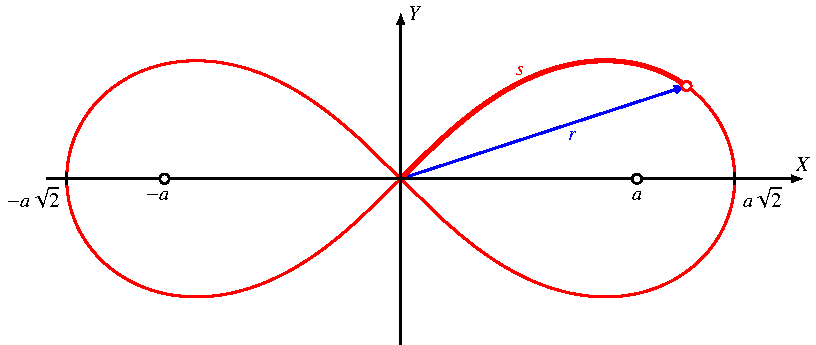
\includegraphics{chapters/110-elliptisch/images/lemniskate.pdf}
\caption{Bogenlänge und Radius der Lemniskate von Bernoulli.
\label{buch:elliptisch:fig:lemniskate}}
\end{figure}
Die Lemniskate von Bernoulli ist die Kurve vierten Grades mit der Gleichung
\begin{equation}
(X^2+Y^2)^2 = 2a^2(X^2-Y^2).
\label{buch:elliptisch:eqn:lemniskate}
\end{equation}
Sie ist in Abbildung~\ref{buch:elliptisch:fig:lemniskate}
dargestellt.
Die beiden Scheitel der Lemniskate befinden sich bei $X_s=\pm a\sqrt{2}$.
Dividiert man die Gleichung der Lemniskate durch $X_s^2=4a^4$ entsteht 
\begin{equation}
\biggl(
\biggl(\frac{X}{a\sqrt{2}}\biggr)^2
+
\biggl(\frac{Y}{a\sqrt{2}}\biggr)^2
\biggr)^2
=
2\frac{a^2}{2a^2}\biggl(
\biggl(\frac{X}{a\sqrt{2}}\biggr)^2
-
\biggl(\frac{Y}{a\sqrt{2}}\biggr)^2
\biggr).
\qquad
\Leftrightarrow
\qquad
(x^2+y^2)^2 = x^2-y^2,
\label{buch:elliptisch:eqn:lemniskatenormiert}
\end{equation}
wobei wir $x=X/a\sqrt{2}$ und $y=Y/a\sqrt{2}$ gesetzt haben.
In dieser Normierung liegen die Scheitel bei $\pm 1$.
Dies ist die Skalierung, die für die Definition des lemniskatischen
Sinus und Kosinus verwendet werden soll.

In Polarkoordinaten $x=r\cos\varphi$ und $y=r\sin\varphi$
gilt nach Einsetzen in \eqref{buch:elliptisch:eqn:lemniskatenormiert}
\begin{equation}
r^4
=
r^2(\cos^2\varphi-\sin^2\varphi)
=
r^2\cos2\varphi
\qquad\Rightarrow\qquad
r^2 = \cos 2\varphi
\label{buch:elliptisch:eqn:lemniskatepolar}
\end{equation}
als Darstellung der Lemniskate in Polardarstellung.
Sie gilt für Winkel $\varphi\in[-\frac{\pi}4,\frac{\pi}4]$ für das
rechte Blatt und $\varphi\in[\frac{3\pi}4,\frac{5\pi}4]$ für das linke
Blatt der Lemniskate.

\subsection{Bogenlänge}
Die Funktionen
\begin{equation}
x(r) = \frac{r}{\sqrt{2}}\sqrt{1+r^2},
\quad
y(r) = \frac{r}{\sqrt{2}}\sqrt{1-r^2}
\label{buch:geometrie:eqn:lemniskateparam}
\end{equation}
erfüllen
\begin{align*}
x(r)^2-y(r)^2
&=
\frac{r^2(1+r^2)}{2}-\frac{r^2(1-r^2)}{2}
\\
&
=
r^4
=
(x(r)^2 + y(r)^2)^2,
\end{align*}
sie stellen also eine Parametrisierung der Lemniskate dar.

Mit Hilfe der Parametrisierung~\eqref{buch:geometrie:eqn:lemniskateparam}
kann man die Länge $s$ des in Abbildung~\ref{buch:elliptisch:fig:lemniskate}
dargestellten Bogens der Lemniskate berechnen.
Dazu benötigt man die Ableitungen nach $r$, die man mit der Produkt- und
Kettenregel berechnen kann:
\begin{align*}
\dot{x}(r)
&=
\frac{\sqrt{1+r^2}}{\sqrt{2}}
+
\frac{r^2}{\sqrt{2}\sqrt{1+r^2}}
&&\Rightarrow&
\dot{x}(r)^2
&=
\frac{1+r^2}{2} +r^2 + \frac{r^4}{2(1+r^2)}
\\
\dot{y}(r)
&=
\frac{\sqrt{1-r^2}}{\sqrt{2}}
-
\frac{r^2}{\sqrt{2}\sqrt{1-r^2}}
&&\Rightarrow&
\dot{y}(r)^2
&=
\frac{1-r^2}{2} -r^2 + \frac{r^4}{2(1-r^2)}
\end{align*}
Die Summe der Quadrate ist
\begin{align*}
\dot{x}(r)^2 + \dot{y}(r)^2
&=
1 + r^4\frac{1-r^2+1+r^2}{2(1+r^2)(1-r^2)}
=
1+r^4\frac{2}{2(1-r^4)}
=
\frac{1-r^4+r^4}{1-r^4}
=
\frac1{1-r^4}.
\end{align*}
Durch Einsetzen in das Integral für die Bogenlänge bekommt man
\begin{equation}
s(r)
=
\int_0^r
\frac{1}{\sqrt{1-t^4}}\,dt.
\label{buch:elliptisch:eqn:lemniskatebogenlaenge}
\end{equation}

%
% Als elliptisches Integral
%
\subsection{Darstellung als elliptisches Integral}
Das unvollständige elliptische Integral erster Art mit Parameter
$k^2=-1$ oder $k=i$ ist
\[
K(r,i)
=
\int_0^x \frac{dt}{\sqrt{(1-t^2)(1-i^2 t^2)}}
=
\int_0^x \frac{dt}{\sqrt{(1-t^2)(1-(-1)t^2)}}
=
\int_0^x \frac{dt}{\sqrt{1-t^4}}
=
s(r).
\]
Der lemniskatische Sinus ist also eine Umkehrfunktion des
elliptischen Integrals erster Art für den speziellen Wert $i$ des
Parameters $k$.

Die Länge des rechten Blattes der Lemniskate wird mit $\varpi$ bezeichnet
und hat den numerischen Wert
\[
\varpi
=
2\int_0^1\sqrt{\frac{1}{1-t^4}}\,dt
=
2.6220575542.
\]
$\varpi$ ist auch als die {\em lemniskatische Konstante} bekannt.
\index{lemniskatische Konstante}%
Der Lemniskatenbogen zwischen dem Nullpunkt und $(1,0)$ hat die Länge
$\varpi/2$.

%
%  Bogenlängenparametrisierung
%
\subsection{Bogenlängenparametrisierung}
Die Lemniskate mit der Gleichung
\[
(X^2+X^2)^2=2(X^2-X^2)
\]
(der Fall $a=1$ in \eqref{buch:elliptisch:eqn:lemniskate})
kann mit Jacobischen elliptischen Funktionen
parametrisiert werden.
Dazu schreibt man
\[
\left.
\begin{aligned}
X(t)
&=
\sqrt{2}\operatorname{cn}(t,k) \operatorname{dn}(t,k)
\\
Y(t)
&=
\phantom{\sqrt{2}}
\operatorname{cn}(t,k) \operatorname{sn}(t,k)
\end{aligned}
\quad\right\}
\qquad\text{mit $k=\displaystyle\frac{1}{\sqrt{2}}$}
\]
und berechnet die beiden Seiten der definierenden Gleichung der
Lemniskate.
Zunächst ist
\begin{align*}
X(t)^2
&=
2\operatorname{cn}(t,k)^2
\operatorname{dn}(t,k)^2
\\
Y(t)^2
&=
\operatorname{cn}(t,k)^2
\operatorname{sn}(t,k)^2
\\
X(t)^2+Y(t)^2
&=
2\operatorname{cn}(t,k)^2
\bigl(
\underbrace{
\operatorname{dn}(t,k)^2
+{\textstyle\frac12}
\operatorname{sn}(t,k)^2
}_{\displaystyle =1}
\bigr)
%\\
%&
=
2\operatorname{cn}(t,k)^2
\\
X(t)^2-Y(t)^2
&=
\operatorname{cn}(t,k)^2
\bigl(
2\operatorname{dn}(t,k)^2 - \operatorname{sn}(t,k)^2
\bigr)
\\
&=
\operatorname{cn}(t,k)^2
\bigl(
2\bigl({\textstyle\frac12}+{\textstyle\frac12}\operatorname{cn}(t,k)^2\bigr)
-
\bigl(1-\operatorname{cn}(t,k)^2\bigr)
\bigr)
\\
&=
2\operatorname{cn}(t,k)^4
\\
\Rightarrow\qquad
(X(t)^2+Y(t)^2)^2
&=
4\operatorname{cn}(t,k)^4
=
2(X(t)^2-Y(t)^2).
\end{align*}
Wir zeigen jetzt, dass dies tatsächlich eine Bogenlängenparametrisierung
der Lemniskate ist.
Dazu berechnen wir die Ableitungen
\begin{align*}
\dot{X}(t)
&=
\sqrt{2}\operatorname{cn}'(t,k)\operatorname{dn}(t,k)
+
\sqrt{2}\operatorname{cn}(t,k)\operatorname{dn}'(t,k)
\\
&=
-\sqrt{2}\operatorname{sn}(t,k)\operatorname{dn}(t,k)^2
-\frac12\sqrt{2}\operatorname{sn}(t,k)\operatorname{cn}(t,k)^2
\\
&=
-\sqrt{2}\operatorname{sn}(t,k)\bigl(
1-{\textstyle\frac12}\operatorname{sn}(t,k)^2
+{\textstyle\frac12}-{\textstyle\frac12}\operatorname{sn}(u,t)^2
\bigr)
\\
&=
\sqrt{2}\operatorname{sn}(t,k)
\bigl(
{\textstyle \frac32}-\operatorname{sn}(t,k)^2
\bigr)
\\
\dot{X}(t)^2
&=
2\operatorname{sn}(t,k)^2
\bigl(
{\textstyle \frac32}-\operatorname{sn}(t,k)^2
\bigr)^2
\\
&=
{\textstyle\frac{9}{2}}\operatorname{sn}(t,k)^2
-
6\operatorname{sn}(t,k)^4
+2\operatorname{sn}(t,k)^6
\\
\dot{Y}(t)
&=
\operatorname{cn}'(t,k)\operatorname{sn}(t,k)
+
\operatorname{cn}(t,k)\operatorname{sn}'(t,k)
\\
&=
-\operatorname{sn}(t,k)^2
\operatorname{dn}(t,k)
+\operatorname{cn}(t,k)^2
\operatorname{dn}(t,k)
\\
&=
\operatorname{dn}(t,k)\bigl(1-2\operatorname{sn}(t,k)^2\bigr)
\\
\dot{Y}(t)^2
&=
\bigl(1-{\textstyle\frac12}\operatorname{sn}(t,k)^2\bigr)
\bigl(1-2\operatorname|{sn}(t,k)^2\bigr)^2
\\
&=
1-{\textstyle\frac{9}{2}}\operatorname{sn}(t,k)^2
+6\operatorname{sn}(t,k)^4
-2\operatorname{sn}(t,k)^6
\\
\dot{X}(t)^2 + \dot{Y}(t)^2
&=
1.
\end{align*}
Dies bedeutet, dass die Bogenlänge zwischen den Parameterwerten $0$ und $s$
\[
\int_0^s
\sqrt{\dot{X}(t)^2 + \dot{Y}(t)^2}
\,dt
=
\int_0^s\,dt
=
s,
\]
der Parameter $t$ ist also ein Bogenlängenparameter.

Die mit dem Faktor $1/\sqrt{2}$ skalierte Standard-Lemniskate mit der
Gleichung
\[
(x^2+y^2)^2 = x^2-y^2
\]
hat daher eine Bogenlängenparametrisierung mit
\begin{equation}
\begin{aligned}
x(t)
&=
\phantom{\frac{1}{\sqrt{2}}}
\operatorname{cn}(\sqrt{2}t,k)\operatorname{dn}(\sqrt{2}t,k)
\\
y(t)
&=
\frac{1}{\sqrt{2}}\operatorname{cn}(\sqrt{2}t,k)\operatorname{sn}(\sqrt{2}t,k)
\end{aligned}
\label{buch:elliptisch:lemniskate:bogenlaenge}
\end{equation}

\subsection{Der lemniskatische Sinus und Kosinus}
Der Sinus Berechnet die Gegenkathete zu einer gegebenen Bogenlänge des
Kreises, er ist die Umkehrfunktion der Funktion, die der Gegenkathete
die Bogenlänge zuordnet.

Daher ist es naheliegend, die Umkehrfunktion von $s(r)$ in 
\eqref{buch:elliptisch:eqn:lemniskatebogenlaenge}
den {\em lemniskatischen Sinus} zu nennen mit der Bezeichnung
$r=\operatorname{sl} s$.

Der Kosinus ist der Sinus des komplementären Winkels.
Auch für die lemniskatische Bogenlänge $s(r)$ lässt sich eine
komplementäre Bogenlänge definieren, nämlich die Bogenlänge zwischen
dem Punkt $(x(r), y(r))$ und $(1,0)$.

Da die Parametrisierung~\eqref{buch:elliptisch:lemniskate:bogenlaenge}
eine Bogenlängenparametrisierung ist, darf man $t=s$ schreiben.
Dann kann man aber auch $r(s)$ daraus berechnen,
es ist
\[
r(s)^2
=
x(s)^2 + y(s)^2
=
\operatorname{cn}(s\sqrt{2},k)^2
\qquad\Rightarrow\qquad
r(s)
=
\operatorname{cn}(s\sqrt{2},k)
\]

\begin{figure}
\centering
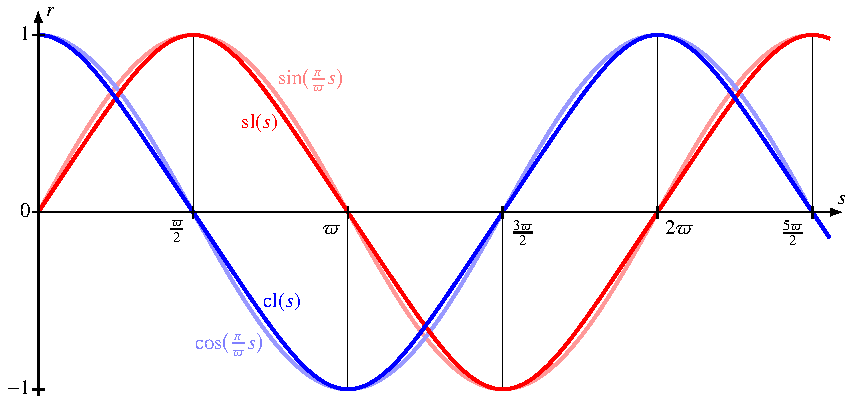
\includegraphics{chapters/110-elliptisch/images/slcl.pdf}
\caption{
Lemniskatischer Sinus und Kosinus sowie Sinus und Kosinus
mit derart skaliertem Argument, dass die Funktionen die gleichen Nullstellen
haben.
\label{buch:elliptisch:figure:slcl}}
\end{figure}


%\section*{Übungsaufgaben}
%\rhead{Übungsaufgaben}
%\aufgabetoplevel{chapters/020-exponential/uebungsaufgaben}
%\begin{uebungsaufgaben}
%\uebungsaufgabe{0}
%\uebungsaufgabe{1}
%\end{uebungsaufgaben}


%
% chapter.tex -- Beschreibung des Inhaltes
%
% (c) 2021 Prof Dr Andreas Müller, Hochschule Rapperswil
%
% !TeX spellcheck = de_CH
\chapter{Elliptische Funktionen
\label{buch:chapter:geometrie}}
\lhead{Elliptische Funktionen}
\rhead{}

Der Versuch, die Länge eines Ellipsenbogens zu berechnen, hat
in Abschnitt~\ref{buch:geometrie:subsection:hyperbeln-und-ellipsen}
zu Integralen geführt, die nicht in geschlossener Form ausgewertet
werden können.
Neben den dort gefundenen Integralen sind noch weitere, ähnlich
aufgebaute Integrale in dieser Familie zu finden.

%
% ellintegral.tex
%
% (c) 2021 Prof Dr Andreas Müller, OST Ostschweizer Fachhochschule
%
\section{Elliptische Integrale
\label{buch:elliptisch:section:integral}}
\rhead{Elliptisches Integral}
Bei der Berechnung des Ellipsenbogens in 
Abschnitt~\ref{buch:geometrie:subsection:hyperbeln-und-ellipsen}
sind wir auf ein Integral gestossen, welches sich nicht in geschlossener
Form ausdrücken liess.
Um solche Integrale in den Griff zu bekommen, ist es nötig, sie als
neue spezielle Funktionen zu definieren.

\subsection{Definition
\label{buch:elliptisch:subsection:definition}}
Ein {\em elliptisches Integral} ist ein Integral der Form
\index{elliptishes Integral}%
\index{Integral, elliptisch}%
\begin{equation}
\int R\left( x, \sqrt{p(x)}\right)\,dx
\label{buch:elliptisch:def:allgemein}
\end{equation}
wobei $R(x,y)$ eine rationale Funktion von zwei Variablen ist und
$p(x)$ ein Polynom dritten oder vierten Grades.
Hätte $p(x)$ ein mehrfache Nullstelle $x_0$, müsste es durch $(x-x_0)^2$
teilbar sein, man könnte also einen Faktor $(x-x_0)$ aus der
Wurzel im Integraneden von \eqref{buch:elliptisch:def:allgemein}
ausklammern und damit das Integral in eine Form bringen, wo $p(x)$
höchstens zweiten Grades ist.
Solche Integrale lassen sich meistens mit trigonometrischen Substitutionen
berechnen.
Wir verlangen daher, dass $p(x)$ keine mehrfachen Nullstellen hat.

Man kann zeigen, dass sich elliptische Integrale in Summen von
elementaren Funktionen und speziellen elliptischen Integralen 
der folgenden Form überführen lassen
\cite[Abschnitt 164, p.~506]{buch:smirnov32}.

\begin{definition}
\label{buch:elliptisch:def:integrale123}
Die elliptischen Integrale erster, zweiter und dritter Art sind die
Integrale
\[
\begin{aligned}
\text{1.~Art:}&&&
\int \frac{dx}{\sqrt{(1-x^2)(1-k^2x^2)}}
\\
\text{2.~Art:}&&&
\int \sqrt{\frac{1-k^2x^2}{1-x^2}}\,dx
\\
\text{3.~Art:}&&&
\int \frac{dx}{(1-nx^2)\sqrt{(1-x^2)(1-k^2x^2)}}
\end{aligned}
\]
mit $0<k<1$.
Es ist auch üblich, den Parameter $m=k^2$ zu verwenden.
\end{definition}

Wie gesagt lassen sich für diese unbestimmten Integrale keine 
geschlossenen Formen finden.
Es bleibt uns daher nichts anderes übrig, als die Integralgrenzen
festzulegen und damit eine Stammfunktion auszuwählen.

%
% Elliptisches Integral
%
\subsection{Vollständige elliptische Integrale
\label{buch:elliptisch:subsection:vollstaendig}}
In diesem Abschnitt legen wir beide Integrationsgrenzen fest und
untersuchen die entstehenenden Funktionen von den Parametern
$k$ und $n$.

\subsubsection{Definition der vollständigen elliptischen Integrale}
Da der Nenner in allen drei elliptischen Integralen eine Nullstelle
bei $\pm1$ hat, kann das Integral nur von $0$ bis $1$ erstreckt werden.

\begin{definition}
\label{buch:elliptisch:def:vollstintegrale123}
Die vollständigen elliptischen Integrale erster, zweiter und dritter
Art sind
\[
\begin{aligned}
\text{1.~Art:}&&
K(k)&=\int_0^1 \frac{dt}{\sqrt{(1-t^2)(1-k^2t^2)}} \\
\text{2.~Art:}&&
E(k)&=\int_0^1 \sqrt{\frac{1-k^2t^2}{1-t^2}}\,dt \\
\text{3.~Art:}&&
\Pi(n, k)&=\int_0^1\frac{dt}{(1-nt^2)\sqrt{(1-t^2)(1-k^2t^2)}} 
\end{aligned}
\]
mit $0<k<1$.
\end{definition}

Die Funktionen hängen stetig von $k$ ab.
Die Nullstellen des Faktors $1-k^2x^2$ liegen ausserhalb des
Integrationsintervalls und spielen daher keine Rolle.
Die Werte von $K(k)$ und $E(k)$ für $k=0$ können direkt berechnet
werden:
\begin{align*}
K(0)
=
E(0)
&=
\int_0^1 \frac{dt}{\sqrt{1-t^2}}=\frac{\pi}2.
\end{align*}
Das Integral $\Pi(n,0)$ ist etwas komplizierter.

Für $k\to 1$ ist $E(k)=1$, die Integrale $K(1)$ und $\Pi(n,1)$
sind dagegen divergent.

\subsubsection{Jacobi- und Legendre-Normalform}
Die Integrationsvariable $t$ der vollständigen elliptischen Integrale
kann durch die Substitution $t=\sin\varphi$ durch die Variable
$\varphi$ und das Integral über das Intervall $[0,1]$ durch ein
Integral über das Intervall $[0,\frac{\pi}2]$ ersetzt werden.
Mit
\[
\frac{dt}{d\varphi} = \cos\varphi = \sqrt{1-\sin^2\varphi}
\]
können die Funktionen $K(k)$, $E(k)$ und $\Pi(n,k)$ auch als
\begin{align*}
K(k)
&=
\int_0^{\frac{\pi}2}
\frac{
\sqrt{1-\sin^2\varphi}\,d\varphi
}{
\sqrt{(1-\sin^2\varphi)(1-k^2\sin^2\varphi)}
}
=
\int_0^{\frac{\pi}2}
\frac{d\varphi}{\sqrt{1-k^2\sin^2\varphi}}
\\
E(k)
&=
\int_0^{\frac{\pi}2}
\sqrt{\frac{1-k^2\sin^2\varphi}{1-\sin^2\varphi}}\sqrt{1-\sin^2\varphi}\,d\varphi
=
\int_0^{\frac{\pi}2}
\sqrt{1-k^2\sin^2\varphi}\,d\varphi
\\
\Pi(n,k)
&=
\int_0^{\frac{\pi}2}
\frac{
\sqrt{1-\sin^2\varphi}\,d\varphi
}{
(1-n\sin^2\varphi)\sqrt{(1-\sin^2\varphi)(1-k^2\sin^2\varphi)}
}
=
\int_0^{\frac{\pi}2}
\frac{
d\varphi
}{
(1-n\sin^2\varphi)\sqrt{1-k^2\sin^2\varphi}
}
\end{align*}
Diese Form wird auch die {\em Legendre-Normalform} der vollständigen 
\index{Legendre-Normalform}%
elliptischen Integrale genannt, während die Form von
Definition~\ref{buch:elliptisch:def:vollstintegrale123}
die {\em Jacobi-Normalform} heisst.
\index{Jacobi-Normalform}%

\subsubsection{Umfang einer Ellipse}
\begin{figure}
\centering
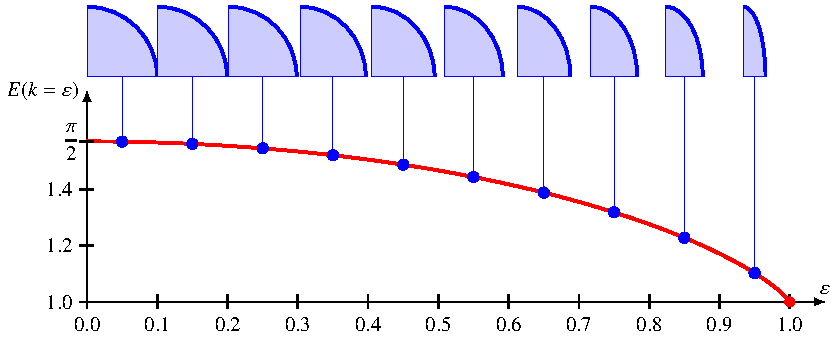
\includegraphics{chapters/110-elliptisch/images/ellipsenumfang.pdf}
\caption{Bogenlänge eines Viertels einer Ellipse mit Exzentrizität
$\varepsilon$.
\label{buch:elliptisch:fig:ellipsenumfang}}
\end{figure}
Wir zeigen, wie sich die Berechnung des Umfangs $U$ einer Ellipse
mit Halbachsen $a$ und $b$, $a\le b$, auf ein volltändiges elliptisches
Integral zurückführen lässt.
Der Fall $a>b$ kann behandelt werden, indem die $x$- und $y$-Koordinaten
vertauscht werden.

Die Parametrisierung
\[
t\mapsto \begin{pmatrix}a\cos t\\ b\sin t\end{pmatrix}
\]
einer Ellipse führt auf das Integral
\begin{align*}
U
&=
\int_0^{2\pi} \sqrt{a^2\sin^2t + b^2\cos^2 t}\,dt
\notag
\\
&=
4\int_0^{\frac{\pi}2}
\sqrt{a^2\sin^2t + b^2(1-\sin^2 t)}
\,dt
\notag
\\
&=
4b \int_0^{\frac{\pi}2} \sqrt{1-(b^2-a^2)/b^2\cdot \sin^2t}\,dt
\label{buch:elliptisch:eqn:umfangellipse}
\end{align*}
für den Umfang der Ellipse.
Bei einem Kreis ist $a=b$ und der zweite Term unter der Wurzel fällt weg,
der Umfang wird $4b\frac{\pi}2=2\pi b$.
Die Differenz $e^2=b^2-a^2$ ist die {\em lineare Exzentrizität} der Ellipse,
\index{lineare Exzentrizität}%
der Quotient $e/b$ wird die {\em numerische Exzentrizität} der Ellipse
genannt.
Insbesondere ist $k = \varepsilon$.

Das Integral~\eqref{buch:elliptisch:eqn:umfangellipse} erhält jetzt die
Form
\[
U
=
4b\int_0^{\frac{\pi}2} \sqrt{1-k^2\sin^2t}\,dt
\]
und ist damit als elliptisches Integral zweiter Art erkannt.
Für den Umfang der Ellipse finden wir damit die Formel
\[
U
=
4b E(k)
=
4b E(\varepsilon).
\]
Das vollständige elliptische Integral zweiter Art $E(\varepsilon)$
liefert also genau den Umfang der eines Viertels Ellipse mit
numerischer Exzentrizität $\varepsilon$ und kleiner Halbachse $1$.

\subsubsection{Komplementäre Integrale}
XXX Komplementäre Integrale \\

\subsubsection{Ableitung}
XXX Ableitung \\
XXX Stammfunktion \\

\subsection{Unvollständige elliptische Integrale}
XXX Vollständige und Unvollständige Integrale \\
XXX Additionstheoreme \\
XXX Parameterkonventionen \\

\subsection{Potenzreihe}
XXX Potenzreihen \\
XXX Als hypergeometrische Funktionen \\



\section{Jacobische elliptische Funktionen}

Für das elliptische Filter werden, wie es der Name bereits deutet, elliptische Funktionen gebraucht.
Wie die trigonometrischen Funktionen Zusammenhänge eines Kreises darlegen, beschreiben die elliptischen Funktionen Ellipsen.
Es ist daher naheliegend, dass der Kosinus des Tschebyscheff-Filters gegen ein elliptisches Pendant ausgetauscht werden könnte.
Der Begriff elliptische Funktion wird für sehr viele Funktionen gebraucht, daher ist es hier wichtig zu erwähnen, dass es ausschliesslich um die Jacobischen elliptischen Funktionen geht.

\subsection{Grundlegende Eigenschaften}

Die Jacobi elliptischen Funktionen werden ausführlich im Kapitel \ref{buch:elliptisch:section:jacobi} behandelt.
Im Wesentlichen erweitern die Jacobi elliptischen Funktionen die trigonometrische Funktionen für Ellipsen.
Zum Beispiel gibt es analog zum Sinus den elliptischen $\sn(z, k)$.
Im Gegensatz zum den trigonometrischen Funktionen haben die elliptischen Funktionen zwei Parameter.
Den \textit{elliptische Modul} $k$, der die Exzentrizität der Ellipse parametrisiert und das Winkelargument $z$.
Im Kreis ist der Radius für alle Winkel konstant, bei Ellipsen ändert sich das.
Dies hat zur Folge, dass bei einer Ellipse die Kreisbogenlänge nicht linear zum Winkel verläuft.
Darum kann hier nicht der gewohnte Winkel verwendet werden.
Das Winkelargument $z$ kann durch das elliptische Integral erster Art
\begin{equation}
    z
    =
    F(\phi, k)
    =
    \int_{0}^{\phi}
    \frac{
        d\theta
    }{
        \sqrt{
            1-k^2 \sin^2 \theta
        }
    }
\end{equation}
mit dem Winkel $\phi$ in Verbindung gebracht werden.

Dabei wird das vollständige und unvollständige elliptische integral unterschieden.
Beim vollständigen Integral
\begin{equation}
    K(k)
    =
    \int_{0}^{\pi / 2}
    \frac{
        d\theta
    }{
        \sqrt{
            1-k^2 \sin^2 \theta
        }
    }
\end{equation}
wird über ein viertel Ellipsenbogen integriert, also bis $\phi=\pi/2$ und liefert das Winkelargument für eine Vierteldrehung.
Die Zahl wird oft auch abgekürzt mit $K = K(k)$ und ist für das elliptische Filter sehr relevant.
Alle elliptischen Funktionen sind somit $4K$-periodisch.

Neben dem $\sn$ gibt es zwei weitere elliptische Basisfunktionen $\cn$ und $\dn$.
Dazu kommen noch weitere abgeleitete Funktionen, die durch Quotienten und Kehrwerte dieser Funktionen zustande kommen.
Insgesamt sind es die zwölf Funktionen
\begin{equation*}
    \sn \quad
    \ns \quad
    \scelliptic \quad
    \sd \quad
    \cn \quad
    \nc \quad
    \cs \quad
    \cd \quad
    \dn \quad
    \nd \quad
    \ds \quad
    \dc.
\end{equation*}

Die Jacobischen elliptischen Funktionen können mit der inversen Funktion des vollständigen elliptischen Integrals erster Art
\begin{equation}
    \phi = F^{-1}(z, k)
\end{equation}
definiert werden. Dabei ist zu beachten dass nur das $z$ Argument der Funktion invertiert wird, also
\begin{equation}
    z = F(\phi, k)
    \Leftrightarrow
    \phi = F^{-1}(z, k).
\end{equation}
Mithilfe von $F^{-1}$ kann zum Beispiel $sn^{-1}$ mit dem elliptischen Integral dargestellt werden:
\begin{equation}
    \sin(\phi)
    =
    \sin \left( F^{-1}(z, k) \right)
    =
    \sn(z, k)
    =
    w.
\end{equation}

% \begin{equation} %TODO remove unnecessary equations
%     \phi
%     =
%      F^{-1}(z, k)
%      =
%      \sin^{-1} \big( \sn (z, k ) \big)
%      =
%     \sin^{-1} ( w )
% \end{equation}

% \begin{equation}
%     F(\phi, k)
%     =
%     z
%     =
%     F( \sin^{-1} \big( \sn (z, k ) \big) , k)
%     =
%     F( \sin^{-1} ( w ), k)
% \end{equation}

% \begin{equation}
%     \sn^{-1}(w, k)
%     =
%     F(\phi, k),
%     \quad
%     \phi = \sin^{-1}(w)
% \end{equation}

\subsection{Die Funktion $\sn^{-1}$}

Beim Tschebyscheff-Filter konnten wir mit Betrachten des Arcuscosinus die Funktionalität erklären.
Für das Elliptische Filter machen wir die gleiche Betrachtung mit der $\sn^{-1}$-Funktion.
Der $\sn^{-1}$ ist durch das elliptische Integral
\begin{align}
    \sn^{-1}(w, k)
        & =
    \int_{0}^{\phi}
    \frac{
        d\theta
    }{
        \sqrt{
            1-k^2 \sin^2 \theta
        }
    },
    \quad
    \phi = \sin^{-1}(w)
    \\
        & =
    \int_{0}^{w}
    \frac{
        dt
    }{
        \sqrt{
            (1-t^2)(1-k^2 t^2)
        }
    }
\end{align}
beschrieben.
Dazu betrachten wir wieder den Integranden
\begin{equation}
    \frac{
        1
    }{
        \sqrt{
            (1-t^2)(1-k^2 t^2)
        }
    }.
\end{equation}
Beim $\cos^{-1}(x)$ haben wir gesehen, dass die analytische Fortsetzung bei $x < -1$ und $x > 1$ rechtwinklig in die komplexen Zahlen wandert.
Wenn man das Gleiche mit $\sn^{-1}(w, k)$ macht, erkennt man zwei interessante Stellen.
Die erste ist die gleiche wie beim $\cos^{-1}(x)$ nämlich bei $t = \pm 1$.
Der erste Term unter der Wurzel wird dann negativ, während der zweite noch positiv ist, da $k \leq 1$.
Ab diesem Punkt knickt die Funktion in die imaginäre Richtung ab.
Bei $t = 1/k$ ist auch der zweite Term negativ und die Funktion verläuft in die negative reelle Richtung.
Abbildung \ref{ellfilter:fig:sn} zeigt den Verlauf der Funktion in der komplexen Ebene.
\begin{figure}
    \centering
    \begin{tikzpicture}[>=stealth', auto, node distance=2cm, scale=1.2]

    \tikzstyle{zero} = [draw, circle, inner sep =0, minimum height=0.15cm]

    \tikzset{pole/.style={cross out, draw=black, minimum size=(0.15cm-\pgflinewidth), inner sep=0pt, outer sep=0pt}}

    \begin{scope}[xscale=0.9, yscale=1.8]

        \draw[gray, ->] (0,-1.5) -- (0,1.5) node[anchor=south]{$\mathrm{Im}~z$};
        \draw[gray, ->] (-5,0) -- (5,0) node[anchor=west]{$\mathrm{Re}~z$};

        \begin{scope}

            \clip(-4.5,-1.25) rectangle (4.5,1.25);

            \fill[yellow!30] (0,0) rectangle (1, 0.5);

            \begin{scope}[xshift=-1cm]

                \foreach \i in {-2,...,2} {
                    \foreach \j in {-2,...,1} {
                        \begin{scope}[xshift=\i*4cm, yshift=\j*1cm]
                            \draw[<-, blue!50] (0, 0) -- (0,0.5);
                            \draw[<-, cyan!50] (1, 0) -- (0,0);
                            \draw[<-, darkgreen!50] (2, 0) -- (1,0);
                            \draw[<-, orange!50] (2,0.5) -- (2, 0);
                            \draw[<-, red!50] (1, 0.5) -- (2,0.5);
                            \draw[<-, purple!50] (0, 0.5) -- (1,0.5);
                            \draw[<-, blue!50] (0,1) -- (0,0.5);
                            \draw[<-, orange!50] (2,0.5) -- (2, 1);
                            \draw[<-, red!50] (3, 0.5) -- (2,0.5);
                            \draw[<-, purple!50] (4, 0.5) -- (3,0.5);
                            \draw[<-, darkgreen!50] (2, 0) -- (3,0);
                            \draw[<-, cyan!50] (3, 0) -- (4,0);
                        \end{scope}
                    }
                }

                % \pause
                \draw[ultra thick, <-, darkgreen] (2, 0) -- (1,0);
                % \pause
                \draw[ultra thick, <-, orange] (2,0.5) -- (2, 0);
                % \pause
                \draw[ultra thick, <-, red] (1, 0.5) -- (2,0.5);
                % \pause
                \draw[ultra thick, <-, blue] (0, 0) -- (0,0.5);
                \draw[ultra thick, <-, purple] (0, 0.5) -- (1,0.5);
                \draw[ultra thick, <-, cyan] (1, 0) -- (0,0);
                % \pause


                \foreach \i in {-2,...,2} {
                    \foreach \j in {-2,...,1} {
                        \begin{scope}[xshift=\i*4cm, yshift=\j*1cm]
                            \node[zero] at ( 1, 0) {};
                            \node[zero] at ( 3, 0) {};
                            \node[pole] at ( 1,0.5) {};
                            \node[pole] at ( 3,0.5) {};
                        \end{scope}
                    }
                }

            \end{scope}

        \end{scope}

        \draw[gray] ( 1,0) +(0,0.1) -- +(0, -0.1) node[inner sep=0, anchor=north] {\small $K$};
        \draw[gray]  (0, 0.5) +(0.1, 0) -- +(-0.1, 0) node[inner sep=0, anchor=east]{\small $jK^\prime$};

    \end{scope}

    \node[zero] at (4,3) (n) {};
    \node[anchor=west] at (n.east) {Zero};
    \node[pole, below=0.25cm of n] (n) {};
    \node[anchor=west] at (n.east) {Pole};

    \begin{scope}[yshift=-4cm, xscale=0.75]

        \draw[gray, ->] (-6,0) -- (6,0) node[anchor=west]{$w$};

        \draw[ultra thick, ->, purple] (-5, 0) -- (-3, 0);
        \draw[ultra thick, ->, blue]      (-3, 0) -- (-2, 0);
        \draw[ultra thick, ->, cyan]       (-2, 0) -- (0, 0);
        \draw[ultra thick, ->, darkgreen]    (0, 0) -- (2, 0);
        \draw[ultra thick, ->, orange] (2, 0) -- (3, 0);
        \draw[ultra thick, ->, red] (3, 0) -- (5, 0);

        \node[anchor=south] at (-5,0) {$-\infty$};
        \node[anchor=south] at (-3,0) {$-1/k$};
        \node[anchor=south] at (-2,0) {$-1$};
        \node[anchor=south] at (0,0) {$0$};
        \node[anchor=south] at (2,0) {$1$};
        \node[anchor=south] at (3,0) {$1/k$};
        \node[anchor=south] at (5,0) {$\infty$};

    \end{scope}


\end{tikzpicture}
    \caption{
        $z$-Ebene der Funktion $z = \sn^{-1}(w, k)$.
        Die Funktion ist in der realen Achse $4K$-periodisch und in der imaginären Achse $2jK^\prime$-periodisch.
    }
    \label{ellfilter:fig:sn}
\end{figure}
In der reellen Richtung ist sie $4K(k)$-periodisch und in der imaginären Richtung $4K^\prime(k)$-periodisch, wobei $K^\prime$ das komplementäre vollständige Elliptische Integral ist:
\begin{equation}
    K^\prime(k)
    =
    \int_{0}^{\pi / 2}
    \frac{
        d\theta
    }{
        \sqrt{
            1-{k^\prime}^2 \sin^2 \theta
        }
    },
    \quad
    k^\prime = \sqrt{1-k^2}.
\end{equation}

%
% lemniskate.tex
%
% (c) 2021 Prof Dr Andreas Müller, OST Ostschweizer Fachhochschule
%
\section{Lemniskatischer Sinus
\label{buch:elliptisch:section:lemniskate}}
\rhead{Lemniskatischer Sinus}
Historisch war der {\em lemniskatische Sinus} die erste ellptische
Funktion, die Gauss bereits als 19-jähriger untersucht, aber nicht 
veröffentlich hat.
In diesem Abschnitt soll die Verbindung zu den Jacobischen
elliptischen Funktionen hergestellt werden.

\subsection{Lemniskate
\label{buch:gemotrie:subsection:lemniskate}}
\begin{figure}
\centering
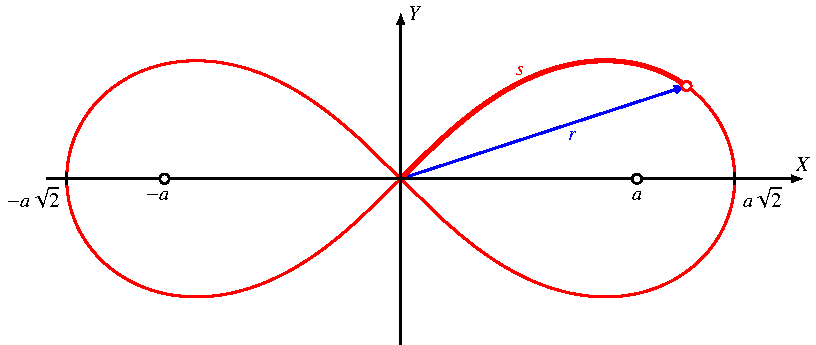
\includegraphics{chapters/110-elliptisch/images/lemniskate.pdf}
\caption{Bogenlänge und Radius der Lemniskate von Bernoulli.
\label{buch:elliptisch:fig:lemniskate}}
\end{figure}
Die Lemniskate von Bernoulli ist die Kurve vierten Grades mit der Gleichung
\begin{equation}
(X^2+Y^2)^2 = 2a^2(X^2-Y^2).
\label{buch:elliptisch:eqn:lemniskate}
\end{equation}
Sie ist in Abbildung~\ref{buch:elliptisch:fig:lemniskate}
dargestellt.
Die beiden Scheitel der Lemniskate befinden sich bei $X_s=\pm a\sqrt{2}$.
Dividiert man die Gleichung der Lemniskate durch $X_s^2=4a^4$ entsteht 
\begin{equation}
\biggl(
\biggl(\frac{X}{a\sqrt{2}}\biggr)^2
+
\biggl(\frac{Y}{a\sqrt{2}}\biggr)^2
\biggr)^2
=
2\frac{a^2}{2a^2}\biggl(
\biggl(\frac{X}{a\sqrt{2}}\biggr)^2
-
\biggl(\frac{Y}{a\sqrt{2}}\biggr)^2
\biggr).
\qquad
\Leftrightarrow
\qquad
(x^2+y^2)^2 = x^2-y^2,
\label{buch:elliptisch:eqn:lemniskatenormiert}
\end{equation}
wobei wir $x=X/a\sqrt{2}$ und $y=Y/a\sqrt{2}$ gesetzt haben.
In dieser Normierung liegen die Scheitel bei $\pm 1$.
Dies ist die Skalierung, die für die Definition des lemniskatischen
Sinus und Kosinus verwendet werden soll.

In Polarkoordinaten $x=r\cos\varphi$ und $y=r\sin\varphi$
gilt nach Einsetzen in \eqref{buch:elliptisch:eqn:lemniskatenormiert}
\begin{equation}
r^4
=
r^2(\cos^2\varphi-\sin^2\varphi)
=
r^2\cos2\varphi
\qquad\Rightarrow\qquad
r^2 = \cos 2\varphi
\label{buch:elliptisch:eqn:lemniskatepolar}
\end{equation}
als Darstellung der Lemniskate in Polardarstellung.
Sie gilt für Winkel $\varphi\in[-\frac{\pi}4,\frac{\pi}4]$ für das
rechte Blatt und $\varphi\in[\frac{3\pi}4,\frac{5\pi}4]$ für das linke
Blatt der Lemniskate.

\subsection{Bogenlänge}
Die Funktionen
\begin{equation}
x(r) = \frac{r}{\sqrt{2}}\sqrt{1+r^2},
\quad
y(r) = \frac{r}{\sqrt{2}}\sqrt{1-r^2}
\label{buch:geometrie:eqn:lemniskateparam}
\end{equation}
erfüllen
\begin{align*}
x(r)^2-y(r)^2
&=
\frac{r^2(1+r^2)}{2}-\frac{r^2(1-r^2)}{2}
\\
&
=
r^4
=
(x(r)^2 + y(r)^2)^2,
\end{align*}
sie stellen also eine Parametrisierung der Lemniskate dar.

Mit Hilfe der Parametrisierung~\eqref{buch:geometrie:eqn:lemniskateparam}
kann man die Länge $s$ des in Abbildung~\ref{buch:elliptisch:fig:lemniskate}
dargestellten Bogens der Lemniskate berechnen.
Dazu benötigt man die Ableitungen nach $r$, die man mit der Produkt- und
Kettenregel berechnen kann:
\begin{align*}
\dot{x}(r)
&=
\frac{\sqrt{1+r^2}}{\sqrt{2}}
+
\frac{r^2}{\sqrt{2}\sqrt{1+r^2}}
&&\Rightarrow&
\dot{x}(r)^2
&=
\frac{1+r^2}{2} +r^2 + \frac{r^4}{2(1+r^2)}
\\
\dot{y}(r)
&=
\frac{\sqrt{1-r^2}}{\sqrt{2}}
-
\frac{r^2}{\sqrt{2}\sqrt{1-r^2}}
&&\Rightarrow&
\dot{y}(r)^2
&=
\frac{1-r^2}{2} -r^2 + \frac{r^4}{2(1-r^2)}
\end{align*}
Die Summe der Quadrate ist
\begin{align*}
\dot{x}(r)^2 + \dot{y}(r)^2
&=
1 + r^4\frac{1-r^2+1+r^2}{2(1+r^2)(1-r^2)}
=
1+r^4\frac{2}{2(1-r^4)}
=
\frac{1-r^4+r^4}{1-r^4}
=
\frac1{1-r^4}.
\end{align*}
Durch Einsetzen in das Integral für die Bogenlänge bekommt man
\begin{equation}
s(r)
=
\int_0^r
\frac{1}{\sqrt{1-t^4}}\,dt.
\label{buch:elliptisch:eqn:lemniskatebogenlaenge}
\end{equation}

%
% Als elliptisches Integral
%
\subsection{Darstellung als elliptisches Integral}
Das unvollständige elliptische Integral erster Art mit Parameter
$k^2=-1$ oder $k=i$ ist
\[
K(r,i)
=
\int_0^x \frac{dt}{\sqrt{(1-t^2)(1-i^2 t^2)}}
=
\int_0^x \frac{dt}{\sqrt{(1-t^2)(1-(-1)t^2)}}
=
\int_0^x \frac{dt}{\sqrt{1-t^4}}
=
s(r).
\]
Der lemniskatische Sinus ist also eine Umkehrfunktion des
elliptischen Integrals erster Art für den speziellen Wert $i$ des
Parameters $k$.

Die Länge des rechten Blattes der Lemniskate wird mit $\varpi$ bezeichnet
und hat den numerischen Wert
\[
\varpi
=
2\int_0^1\sqrt{\frac{1}{1-t^4}}\,dt
=
2.6220575542.
\]
$\varpi$ ist auch als die {\em lemniskatische Konstante} bekannt.
\index{lemniskatische Konstante}%
Der Lemniskatenbogen zwischen dem Nullpunkt und $(1,0)$ hat die Länge
$\varpi/2$.

%
%  Bogenlängenparametrisierung
%
\subsection{Bogenlängenparametrisierung}
Die Lemniskate mit der Gleichung
\[
(X^2+X^2)^2=2(X^2-X^2)
\]
(der Fall $a=1$ in \eqref{buch:elliptisch:eqn:lemniskate})
kann mit Jacobischen elliptischen Funktionen
parametrisiert werden.
Dazu schreibt man
\[
\left.
\begin{aligned}
X(t)
&=
\sqrt{2}\operatorname{cn}(t,k) \operatorname{dn}(t,k)
\\
Y(t)
&=
\phantom{\sqrt{2}}
\operatorname{cn}(t,k) \operatorname{sn}(t,k)
\end{aligned}
\quad\right\}
\qquad\text{mit $k=\displaystyle\frac{1}{\sqrt{2}}$}
\]
und berechnet die beiden Seiten der definierenden Gleichung der
Lemniskate.
Zunächst ist
\begin{align*}
X(t)^2
&=
2\operatorname{cn}(t,k)^2
\operatorname{dn}(t,k)^2
\\
Y(t)^2
&=
\operatorname{cn}(t,k)^2
\operatorname{sn}(t,k)^2
\\
X(t)^2+Y(t)^2
&=
2\operatorname{cn}(t,k)^2
\bigl(
\underbrace{
\operatorname{dn}(t,k)^2
+{\textstyle\frac12}
\operatorname{sn}(t,k)^2
}_{\displaystyle =1}
\bigr)
%\\
%&
=
2\operatorname{cn}(t,k)^2
\\
X(t)^2-Y(t)^2
&=
\operatorname{cn}(t,k)^2
\bigl(
2\operatorname{dn}(t,k)^2 - \operatorname{sn}(t,k)^2
\bigr)
\\
&=
\operatorname{cn}(t,k)^2
\bigl(
2\bigl({\textstyle\frac12}+{\textstyle\frac12}\operatorname{cn}(t,k)^2\bigr)
-
\bigl(1-\operatorname{cn}(t,k)^2\bigr)
\bigr)
\\
&=
2\operatorname{cn}(t,k)^4
\\
\Rightarrow\qquad
(X(t)^2+Y(t)^2)^2
&=
4\operatorname{cn}(t,k)^4
=
2(X(t)^2-Y(t)^2).
\end{align*}
Wir zeigen jetzt, dass dies tatsächlich eine Bogenlängenparametrisierung
der Lemniskate ist.
Dazu berechnen wir die Ableitungen
\begin{align*}
\dot{X}(t)
&=
\sqrt{2}\operatorname{cn}'(t,k)\operatorname{dn}(t,k)
+
\sqrt{2}\operatorname{cn}(t,k)\operatorname{dn}'(t,k)
\\
&=
-\sqrt{2}\operatorname{sn}(t,k)\operatorname{dn}(t,k)^2
-\frac12\sqrt{2}\operatorname{sn}(t,k)\operatorname{cn}(t,k)^2
\\
&=
-\sqrt{2}\operatorname{sn}(t,k)\bigl(
1-{\textstyle\frac12}\operatorname{sn}(t,k)^2
+{\textstyle\frac12}-{\textstyle\frac12}\operatorname{sn}(u,t)^2
\bigr)
\\
&=
\sqrt{2}\operatorname{sn}(t,k)
\bigl(
{\textstyle \frac32}-\operatorname{sn}(t,k)^2
\bigr)
\\
\dot{X}(t)^2
&=
2\operatorname{sn}(t,k)^2
\bigl(
{\textstyle \frac32}-\operatorname{sn}(t,k)^2
\bigr)^2
\\
&=
{\textstyle\frac{9}{2}}\operatorname{sn}(t,k)^2
-
6\operatorname{sn}(t,k)^4
+2\operatorname{sn}(t,k)^6
\\
\dot{Y}(t)
&=
\operatorname{cn}'(t,k)\operatorname{sn}(t,k)
+
\operatorname{cn}(t,k)\operatorname{sn}'(t,k)
\\
&=
-\operatorname{sn}(t,k)^2
\operatorname{dn}(t,k)
+\operatorname{cn}(t,k)^2
\operatorname{dn}(t,k)
\\
&=
\operatorname{dn}(t,k)\bigl(1-2\operatorname{sn}(t,k)^2\bigr)
\\
\dot{Y}(t)^2
&=
\bigl(1-{\textstyle\frac12}\operatorname{sn}(t,k)^2\bigr)
\bigl(1-2\operatorname|{sn}(t,k)^2\bigr)^2
\\
&=
1-{\textstyle\frac{9}{2}}\operatorname{sn}(t,k)^2
+6\operatorname{sn}(t,k)^4
-2\operatorname{sn}(t,k)^6
\\
\dot{X}(t)^2 + \dot{Y}(t)^2
&=
1.
\end{align*}
Dies bedeutet, dass die Bogenlänge zwischen den Parameterwerten $0$ und $s$
\[
\int_0^s
\sqrt{\dot{X}(t)^2 + \dot{Y}(t)^2}
\,dt
=
\int_0^s\,dt
=
s,
\]
der Parameter $t$ ist also ein Bogenlängenparameter.

Die mit dem Faktor $1/\sqrt{2}$ skalierte Standard-Lemniskate mit der
Gleichung
\[
(x^2+y^2)^2 = x^2-y^2
\]
hat daher eine Bogenlängenparametrisierung mit
\begin{equation}
\begin{aligned}
x(t)
&=
\phantom{\frac{1}{\sqrt{2}}}
\operatorname{cn}(\sqrt{2}t,k)\operatorname{dn}(\sqrt{2}t,k)
\\
y(t)
&=
\frac{1}{\sqrt{2}}\operatorname{cn}(\sqrt{2}t,k)\operatorname{sn}(\sqrt{2}t,k)
\end{aligned}
\label{buch:elliptisch:lemniskate:bogenlaenge}
\end{equation}

\subsection{Der lemniskatische Sinus und Kosinus}
Der Sinus Berechnet die Gegenkathete zu einer gegebenen Bogenlänge des
Kreises, er ist die Umkehrfunktion der Funktion, die der Gegenkathete
die Bogenlänge zuordnet.

Daher ist es naheliegend, die Umkehrfunktion von $s(r)$ in 
\eqref{buch:elliptisch:eqn:lemniskatebogenlaenge}
den {\em lemniskatischen Sinus} zu nennen mit der Bezeichnung
$r=\operatorname{sl} s$.

Der Kosinus ist der Sinus des komplementären Winkels.
Auch für die lemniskatische Bogenlänge $s(r)$ lässt sich eine
komplementäre Bogenlänge definieren, nämlich die Bogenlänge zwischen
dem Punkt $(x(r), y(r))$ und $(1,0)$.

Da die Parametrisierung~\eqref{buch:elliptisch:lemniskate:bogenlaenge}
eine Bogenlängenparametrisierung ist, darf man $t=s$ schreiben.
Dann kann man aber auch $r(s)$ daraus berechnen,
es ist
\[
r(s)^2
=
x(s)^2 + y(s)^2
=
\operatorname{cn}(s\sqrt{2},k)^2
\qquad\Rightarrow\qquad
r(s)
=
\operatorname{cn}(s\sqrt{2},k)
\]

\begin{figure}
\centering
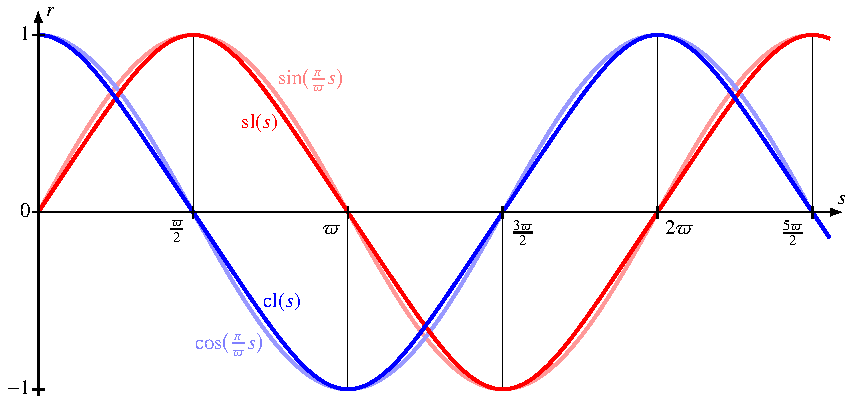
\includegraphics{chapters/110-elliptisch/images/slcl.pdf}
\caption{
Lemniskatischer Sinus und Kosinus sowie Sinus und Kosinus
mit derart skaliertem Argument, dass die Funktionen die gleichen Nullstellen
haben.
\label{buch:elliptisch:figure:slcl}}
\end{figure}


%\section*{Übungsaufgaben}
%\rhead{Übungsaufgaben}
%\aufgabetoplevel{chapters/020-exponential/uebungsaufgaben}
%\begin{uebungsaufgaben}
%\uebungsaufgabe{0}
%\uebungsaufgabe{1}
%\end{uebungsaufgaben}


%
% chapter.tex -- Beschreibung des Inhaltes
%
% (c) 2021 Prof Dr Andreas Müller, Hochschule Rapperswil
%
% !TeX spellcheck = de_CH
\chapter{Elliptische Funktionen
\label{buch:chapter:geometrie}}
\lhead{Elliptische Funktionen}
\rhead{}

Der Versuch, die Länge eines Ellipsenbogens zu berechnen, hat
in Abschnitt~\ref{buch:geometrie:subsection:hyperbeln-und-ellipsen}
zu Integralen geführt, die nicht in geschlossener Form ausgewertet
werden können.
Neben den dort gefundenen Integralen sind noch weitere, ähnlich
aufgebaute Integrale in dieser Familie zu finden.

%
% ellintegral.tex
%
% (c) 2021 Prof Dr Andreas Müller, OST Ostschweizer Fachhochschule
%
\section{Elliptische Integrale
\label{buch:elliptisch:section:integral}}
\rhead{Elliptisches Integral}
Bei der Berechnung des Ellipsenbogens in 
Abschnitt~\ref{buch:geometrie:subsection:hyperbeln-und-ellipsen}
sind wir auf ein Integral gestossen, welches sich nicht in geschlossener
Form ausdrücken liess.
Um solche Integrale in den Griff zu bekommen, ist es nötig, sie als
neue spezielle Funktionen zu definieren.

\subsection{Definition
\label{buch:elliptisch:subsection:definition}}
Ein {\em elliptisches Integral} ist ein Integral der Form
\index{elliptishes Integral}%
\index{Integral, elliptisch}%
\begin{equation}
\int R\left( x, \sqrt{p(x)}\right)\,dx
\label{buch:elliptisch:def:allgemein}
\end{equation}
wobei $R(x,y)$ eine rationale Funktion von zwei Variablen ist und
$p(x)$ ein Polynom dritten oder vierten Grades.
Hätte $p(x)$ ein mehrfache Nullstelle $x_0$, müsste es durch $(x-x_0)^2$
teilbar sein, man könnte also einen Faktor $(x-x_0)$ aus der
Wurzel im Integraneden von \eqref{buch:elliptisch:def:allgemein}
ausklammern und damit das Integral in eine Form bringen, wo $p(x)$
höchstens zweiten Grades ist.
Solche Integrale lassen sich meistens mit trigonometrischen Substitutionen
berechnen.
Wir verlangen daher, dass $p(x)$ keine mehrfachen Nullstellen hat.

Man kann zeigen, dass sich elliptische Integrale in Summen von
elementaren Funktionen und speziellen elliptischen Integralen 
der folgenden Form überführen lassen
\cite[Abschnitt 164, p.~506]{buch:smirnov32}.

\begin{definition}
\label{buch:elliptisch:def:integrale123}
Die elliptischen Integrale erster, zweiter und dritter Art sind die
Integrale
\[
\begin{aligned}
\text{1.~Art:}&&&
\int \frac{dx}{\sqrt{(1-x^2)(1-k^2x^2)}}
\\
\text{2.~Art:}&&&
\int \sqrt{\frac{1-k^2x^2}{1-x^2}}\,dx
\\
\text{3.~Art:}&&&
\int \frac{dx}{(1-nx^2)\sqrt{(1-x^2)(1-k^2x^2)}}
\end{aligned}
\]
mit $0<k<1$.
Es ist auch üblich, den Parameter $m=k^2$ zu verwenden.
\end{definition}

Wie gesagt lassen sich für diese unbestimmten Integrale keine 
geschlossenen Formen finden.
Es bleibt uns daher nichts anderes übrig, als die Integralgrenzen
festzulegen und damit eine Stammfunktion auszuwählen.

%
% Elliptisches Integral
%
\subsection{Vollständige elliptische Integrale
\label{buch:elliptisch:subsection:vollstaendig}}
In diesem Abschnitt legen wir beide Integrationsgrenzen fest und
untersuchen die entstehenenden Funktionen von den Parametern
$k$ und $n$.

\subsubsection{Definition der vollständigen elliptischen Integrale}
Da der Nenner in allen drei elliptischen Integralen eine Nullstelle
bei $\pm1$ hat, kann das Integral nur von $0$ bis $1$ erstreckt werden.

\begin{definition}
\label{buch:elliptisch:def:vollstintegrale123}
Die vollständigen elliptischen Integrale erster, zweiter und dritter
Art sind
\[
\begin{aligned}
\text{1.~Art:}&&
K(k)&=\int_0^1 \frac{dt}{\sqrt{(1-t^2)(1-k^2t^2)}} \\
\text{2.~Art:}&&
E(k)&=\int_0^1 \sqrt{\frac{1-k^2t^2}{1-t^2}}\,dt \\
\text{3.~Art:}&&
\Pi(n, k)&=\int_0^1\frac{dt}{(1-nt^2)\sqrt{(1-t^2)(1-k^2t^2)}} 
\end{aligned}
\]
mit $0<k<1$.
\end{definition}

Die Funktionen hängen stetig von $k$ ab.
Die Nullstellen des Faktors $1-k^2x^2$ liegen ausserhalb des
Integrationsintervalls und spielen daher keine Rolle.
Die Werte von $K(k)$ und $E(k)$ für $k=0$ können direkt berechnet
werden:
\begin{align*}
K(0)
=
E(0)
&=
\int_0^1 \frac{dt}{\sqrt{1-t^2}}=\frac{\pi}2.
\end{align*}
Das Integral $\Pi(n,0)$ ist etwas komplizierter.

Für $k\to 1$ ist $E(k)=1$, die Integrale $K(1)$ und $\Pi(n,1)$
sind dagegen divergent.

\subsubsection{Jacobi- und Legendre-Normalform}
Die Integrationsvariable $t$ der vollständigen elliptischen Integrale
kann durch die Substitution $t=\sin\varphi$ durch die Variable
$\varphi$ und das Integral über das Intervall $[0,1]$ durch ein
Integral über das Intervall $[0,\frac{\pi}2]$ ersetzt werden.
Mit
\[
\frac{dt}{d\varphi} = \cos\varphi = \sqrt{1-\sin^2\varphi}
\]
können die Funktionen $K(k)$, $E(k)$ und $\Pi(n,k)$ auch als
\begin{align*}
K(k)
&=
\int_0^{\frac{\pi}2}
\frac{
\sqrt{1-\sin^2\varphi}\,d\varphi
}{
\sqrt{(1-\sin^2\varphi)(1-k^2\sin^2\varphi)}
}
=
\int_0^{\frac{\pi}2}
\frac{d\varphi}{\sqrt{1-k^2\sin^2\varphi}}
\\
E(k)
&=
\int_0^{\frac{\pi}2}
\sqrt{\frac{1-k^2\sin^2\varphi}{1-\sin^2\varphi}}\sqrt{1-\sin^2\varphi}\,d\varphi
=
\int_0^{\frac{\pi}2}
\sqrt{1-k^2\sin^2\varphi}\,d\varphi
\\
\Pi(n,k)
&=
\int_0^{\frac{\pi}2}
\frac{
\sqrt{1-\sin^2\varphi}\,d\varphi
}{
(1-n\sin^2\varphi)\sqrt{(1-\sin^2\varphi)(1-k^2\sin^2\varphi)}
}
=
\int_0^{\frac{\pi}2}
\frac{
d\varphi
}{
(1-n\sin^2\varphi)\sqrt{1-k^2\sin^2\varphi}
}
\end{align*}
Diese Form wird auch die {\em Legendre-Normalform} der vollständigen 
\index{Legendre-Normalform}%
elliptischen Integrale genannt, während die Form von
Definition~\ref{buch:elliptisch:def:vollstintegrale123}
die {\em Jacobi-Normalform} heisst.
\index{Jacobi-Normalform}%

\subsubsection{Umfang einer Ellipse}
\begin{figure}
\centering
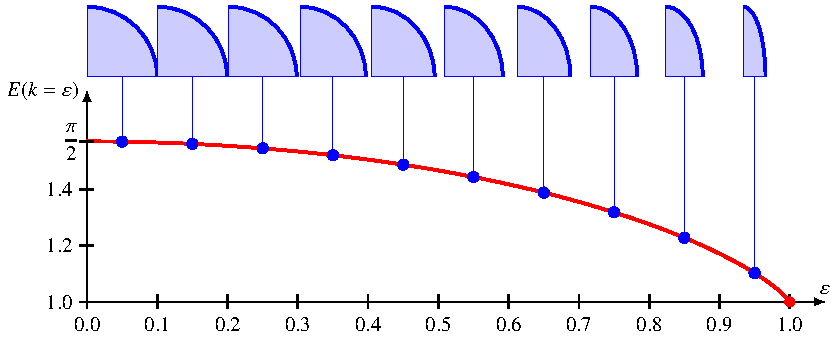
\includegraphics{chapters/110-elliptisch/images/ellipsenumfang.pdf}
\caption{Bogenlänge eines Viertels einer Ellipse mit Exzentrizität
$\varepsilon$.
\label{buch:elliptisch:fig:ellipsenumfang}}
\end{figure}
Wir zeigen, wie sich die Berechnung des Umfangs $U$ einer Ellipse
mit Halbachsen $a$ und $b$, $a\le b$, auf ein volltändiges elliptisches
Integral zurückführen lässt.
Der Fall $a>b$ kann behandelt werden, indem die $x$- und $y$-Koordinaten
vertauscht werden.

Die Parametrisierung
\[
t\mapsto \begin{pmatrix}a\cos t\\ b\sin t\end{pmatrix}
\]
einer Ellipse führt auf das Integral
\begin{align*}
U
&=
\int_0^{2\pi} \sqrt{a^2\sin^2t + b^2\cos^2 t}\,dt
\notag
\\
&=
4\int_0^{\frac{\pi}2}
\sqrt{a^2\sin^2t + b^2(1-\sin^2 t)}
\,dt
\notag
\\
&=
4b \int_0^{\frac{\pi}2} \sqrt{1-(b^2-a^2)/b^2\cdot \sin^2t}\,dt
\label{buch:elliptisch:eqn:umfangellipse}
\end{align*}
für den Umfang der Ellipse.
Bei einem Kreis ist $a=b$ und der zweite Term unter der Wurzel fällt weg,
der Umfang wird $4b\frac{\pi}2=2\pi b$.
Die Differenz $e^2=b^2-a^2$ ist die {\em lineare Exzentrizität} der Ellipse,
\index{lineare Exzentrizität}%
der Quotient $e/b$ wird die {\em numerische Exzentrizität} der Ellipse
genannt.
Insbesondere ist $k = \varepsilon$.

Das Integral~\eqref{buch:elliptisch:eqn:umfangellipse} erhält jetzt die
Form
\[
U
=
4b\int_0^{\frac{\pi}2} \sqrt{1-k^2\sin^2t}\,dt
\]
und ist damit als elliptisches Integral zweiter Art erkannt.
Für den Umfang der Ellipse finden wir damit die Formel
\[
U
=
4b E(k)
=
4b E(\varepsilon).
\]
Das vollständige elliptische Integral zweiter Art $E(\varepsilon)$
liefert also genau den Umfang der eines Viertels Ellipse mit
numerischer Exzentrizität $\varepsilon$ und kleiner Halbachse $1$.

\subsubsection{Komplementäre Integrale}
XXX Komplementäre Integrale \\

\subsubsection{Ableitung}
XXX Ableitung \\
XXX Stammfunktion \\

\subsection{Unvollständige elliptische Integrale}
XXX Vollständige und Unvollständige Integrale \\
XXX Additionstheoreme \\
XXX Parameterkonventionen \\

\subsection{Potenzreihe}
XXX Potenzreihen \\
XXX Als hypergeometrische Funktionen \\



\section{Jacobische elliptische Funktionen}

Für das elliptische Filter werden, wie es der Name bereits deutet, elliptische Funktionen gebraucht.
Wie die trigonometrischen Funktionen Zusammenhänge eines Kreises darlegen, beschreiben die elliptischen Funktionen Ellipsen.
Es ist daher naheliegend, dass der Kosinus des Tschebyscheff-Filters gegen ein elliptisches Pendant ausgetauscht werden könnte.
Der Begriff elliptische Funktion wird für sehr viele Funktionen gebraucht, daher ist es hier wichtig zu erwähnen, dass es ausschliesslich um die Jacobischen elliptischen Funktionen geht.

\subsection{Grundlegende Eigenschaften}

Die Jacobi elliptischen Funktionen werden ausführlich im Kapitel \ref{buch:elliptisch:section:jacobi} behandelt.
Im Wesentlichen erweitern die Jacobi elliptischen Funktionen die trigonometrische Funktionen für Ellipsen.
Zum Beispiel gibt es analog zum Sinus den elliptischen $\sn(z, k)$.
Im Gegensatz zum den trigonometrischen Funktionen haben die elliptischen Funktionen zwei Parameter.
Den \textit{elliptische Modul} $k$, der die Exzentrizität der Ellipse parametrisiert und das Winkelargument $z$.
Im Kreis ist der Radius für alle Winkel konstant, bei Ellipsen ändert sich das.
Dies hat zur Folge, dass bei einer Ellipse die Kreisbogenlänge nicht linear zum Winkel verläuft.
Darum kann hier nicht der gewohnte Winkel verwendet werden.
Das Winkelargument $z$ kann durch das elliptische Integral erster Art
\begin{equation}
    z
    =
    F(\phi, k)
    =
    \int_{0}^{\phi}
    \frac{
        d\theta
    }{
        \sqrt{
            1-k^2 \sin^2 \theta
        }
    }
\end{equation}
mit dem Winkel $\phi$ in Verbindung gebracht werden.

Dabei wird das vollständige und unvollständige elliptische integral unterschieden.
Beim vollständigen Integral
\begin{equation}
    K(k)
    =
    \int_{0}^{\pi / 2}
    \frac{
        d\theta
    }{
        \sqrt{
            1-k^2 \sin^2 \theta
        }
    }
\end{equation}
wird über ein viertel Ellipsenbogen integriert, also bis $\phi=\pi/2$ und liefert das Winkelargument für eine Vierteldrehung.
Die Zahl wird oft auch abgekürzt mit $K = K(k)$ und ist für das elliptische Filter sehr relevant.
Alle elliptischen Funktionen sind somit $4K$-periodisch.

Neben dem $\sn$ gibt es zwei weitere elliptische Basisfunktionen $\cn$ und $\dn$.
Dazu kommen noch weitere abgeleitete Funktionen, die durch Quotienten und Kehrwerte dieser Funktionen zustande kommen.
Insgesamt sind es die zwölf Funktionen
\begin{equation*}
    \sn \quad
    \ns \quad
    \scelliptic \quad
    \sd \quad
    \cn \quad
    \nc \quad
    \cs \quad
    \cd \quad
    \dn \quad
    \nd \quad
    \ds \quad
    \dc.
\end{equation*}

Die Jacobischen elliptischen Funktionen können mit der inversen Funktion des vollständigen elliptischen Integrals erster Art
\begin{equation}
    \phi = F^{-1}(z, k)
\end{equation}
definiert werden. Dabei ist zu beachten dass nur das $z$ Argument der Funktion invertiert wird, also
\begin{equation}
    z = F(\phi, k)
    \Leftrightarrow
    \phi = F^{-1}(z, k).
\end{equation}
Mithilfe von $F^{-1}$ kann zum Beispiel $sn^{-1}$ mit dem elliptischen Integral dargestellt werden:
\begin{equation}
    \sin(\phi)
    =
    \sin \left( F^{-1}(z, k) \right)
    =
    \sn(z, k)
    =
    w.
\end{equation}

% \begin{equation} %TODO remove unnecessary equations
%     \phi
%     =
%      F^{-1}(z, k)
%      =
%      \sin^{-1} \big( \sn (z, k ) \big)
%      =
%     \sin^{-1} ( w )
% \end{equation}

% \begin{equation}
%     F(\phi, k)
%     =
%     z
%     =
%     F( \sin^{-1} \big( \sn (z, k ) \big) , k)
%     =
%     F( \sin^{-1} ( w ), k)
% \end{equation}

% \begin{equation}
%     \sn^{-1}(w, k)
%     =
%     F(\phi, k),
%     \quad
%     \phi = \sin^{-1}(w)
% \end{equation}

\subsection{Die Funktion $\sn^{-1}$}

Beim Tschebyscheff-Filter konnten wir mit Betrachten des Arcuscosinus die Funktionalität erklären.
Für das Elliptische Filter machen wir die gleiche Betrachtung mit der $\sn^{-1}$-Funktion.
Der $\sn^{-1}$ ist durch das elliptische Integral
\begin{align}
    \sn^{-1}(w, k)
        & =
    \int_{0}^{\phi}
    \frac{
        d\theta
    }{
        \sqrt{
            1-k^2 \sin^2 \theta
        }
    },
    \quad
    \phi = \sin^{-1}(w)
    \\
        & =
    \int_{0}^{w}
    \frac{
        dt
    }{
        \sqrt{
            (1-t^2)(1-k^2 t^2)
        }
    }
\end{align}
beschrieben.
Dazu betrachten wir wieder den Integranden
\begin{equation}
    \frac{
        1
    }{
        \sqrt{
            (1-t^2)(1-k^2 t^2)
        }
    }.
\end{equation}
Beim $\cos^{-1}(x)$ haben wir gesehen, dass die analytische Fortsetzung bei $x < -1$ und $x > 1$ rechtwinklig in die komplexen Zahlen wandert.
Wenn man das Gleiche mit $\sn^{-1}(w, k)$ macht, erkennt man zwei interessante Stellen.
Die erste ist die gleiche wie beim $\cos^{-1}(x)$ nämlich bei $t = \pm 1$.
Der erste Term unter der Wurzel wird dann negativ, während der zweite noch positiv ist, da $k \leq 1$.
Ab diesem Punkt knickt die Funktion in die imaginäre Richtung ab.
Bei $t = 1/k$ ist auch der zweite Term negativ und die Funktion verläuft in die negative reelle Richtung.
Abbildung \ref{ellfilter:fig:sn} zeigt den Verlauf der Funktion in der komplexen Ebene.
\begin{figure}
    \centering
    \begin{tikzpicture}[>=stealth', auto, node distance=2cm, scale=1.2]

    \tikzstyle{zero} = [draw, circle, inner sep =0, minimum height=0.15cm]

    \tikzset{pole/.style={cross out, draw=black, minimum size=(0.15cm-\pgflinewidth), inner sep=0pt, outer sep=0pt}}

    \begin{scope}[xscale=0.9, yscale=1.8]

        \draw[gray, ->] (0,-1.5) -- (0,1.5) node[anchor=south]{$\mathrm{Im}~z$};
        \draw[gray, ->] (-5,0) -- (5,0) node[anchor=west]{$\mathrm{Re}~z$};

        \begin{scope}

            \clip(-4.5,-1.25) rectangle (4.5,1.25);

            \fill[yellow!30] (0,0) rectangle (1, 0.5);

            \begin{scope}[xshift=-1cm]

                \foreach \i in {-2,...,2} {
                    \foreach \j in {-2,...,1} {
                        \begin{scope}[xshift=\i*4cm, yshift=\j*1cm]
                            \draw[<-, blue!50] (0, 0) -- (0,0.5);
                            \draw[<-, cyan!50] (1, 0) -- (0,0);
                            \draw[<-, darkgreen!50] (2, 0) -- (1,0);
                            \draw[<-, orange!50] (2,0.5) -- (2, 0);
                            \draw[<-, red!50] (1, 0.5) -- (2,0.5);
                            \draw[<-, purple!50] (0, 0.5) -- (1,0.5);
                            \draw[<-, blue!50] (0,1) -- (0,0.5);
                            \draw[<-, orange!50] (2,0.5) -- (2, 1);
                            \draw[<-, red!50] (3, 0.5) -- (2,0.5);
                            \draw[<-, purple!50] (4, 0.5) -- (3,0.5);
                            \draw[<-, darkgreen!50] (2, 0) -- (3,0);
                            \draw[<-, cyan!50] (3, 0) -- (4,0);
                        \end{scope}
                    }
                }

                % \pause
                \draw[ultra thick, <-, darkgreen] (2, 0) -- (1,0);
                % \pause
                \draw[ultra thick, <-, orange] (2,0.5) -- (2, 0);
                % \pause
                \draw[ultra thick, <-, red] (1, 0.5) -- (2,0.5);
                % \pause
                \draw[ultra thick, <-, blue] (0, 0) -- (0,0.5);
                \draw[ultra thick, <-, purple] (0, 0.5) -- (1,0.5);
                \draw[ultra thick, <-, cyan] (1, 0) -- (0,0);
                % \pause


                \foreach \i in {-2,...,2} {
                    \foreach \j in {-2,...,1} {
                        \begin{scope}[xshift=\i*4cm, yshift=\j*1cm]
                            \node[zero] at ( 1, 0) {};
                            \node[zero] at ( 3, 0) {};
                            \node[pole] at ( 1,0.5) {};
                            \node[pole] at ( 3,0.5) {};
                        \end{scope}
                    }
                }

            \end{scope}

        \end{scope}

        \draw[gray] ( 1,0) +(0,0.1) -- +(0, -0.1) node[inner sep=0, anchor=north] {\small $K$};
        \draw[gray]  (0, 0.5) +(0.1, 0) -- +(-0.1, 0) node[inner sep=0, anchor=east]{\small $jK^\prime$};

    \end{scope}

    \node[zero] at (4,3) (n) {};
    \node[anchor=west] at (n.east) {Zero};
    \node[pole, below=0.25cm of n] (n) {};
    \node[anchor=west] at (n.east) {Pole};

    \begin{scope}[yshift=-4cm, xscale=0.75]

        \draw[gray, ->] (-6,0) -- (6,0) node[anchor=west]{$w$};

        \draw[ultra thick, ->, purple] (-5, 0) -- (-3, 0);
        \draw[ultra thick, ->, blue]      (-3, 0) -- (-2, 0);
        \draw[ultra thick, ->, cyan]       (-2, 0) -- (0, 0);
        \draw[ultra thick, ->, darkgreen]    (0, 0) -- (2, 0);
        \draw[ultra thick, ->, orange] (2, 0) -- (3, 0);
        \draw[ultra thick, ->, red] (3, 0) -- (5, 0);

        \node[anchor=south] at (-5,0) {$-\infty$};
        \node[anchor=south] at (-3,0) {$-1/k$};
        \node[anchor=south] at (-2,0) {$-1$};
        \node[anchor=south] at (0,0) {$0$};
        \node[anchor=south] at (2,0) {$1$};
        \node[anchor=south] at (3,0) {$1/k$};
        \node[anchor=south] at (5,0) {$\infty$};

    \end{scope}


\end{tikzpicture}
    \caption{
        $z$-Ebene der Funktion $z = \sn^{-1}(w, k)$.
        Die Funktion ist in der realen Achse $4K$-periodisch und in der imaginären Achse $2jK^\prime$-periodisch.
    }
    \label{ellfilter:fig:sn}
\end{figure}
In der reellen Richtung ist sie $4K(k)$-periodisch und in der imaginären Richtung $4K^\prime(k)$-periodisch, wobei $K^\prime$ das komplementäre vollständige Elliptische Integral ist:
\begin{equation}
    K^\prime(k)
    =
    \int_{0}^{\pi / 2}
    \frac{
        d\theta
    }{
        \sqrt{
            1-{k^\prime}^2 \sin^2 \theta
        }
    },
    \quad
    k^\prime = \sqrt{1-k^2}.
\end{equation}

%
% lemniskate.tex
%
% (c) 2021 Prof Dr Andreas Müller, OST Ostschweizer Fachhochschule
%
\section{Lemniskatischer Sinus
\label{buch:elliptisch:section:lemniskate}}
\rhead{Lemniskatischer Sinus}
Historisch war der {\em lemniskatische Sinus} die erste ellptische
Funktion, die Gauss bereits als 19-jähriger untersucht, aber nicht 
veröffentlich hat.
In diesem Abschnitt soll die Verbindung zu den Jacobischen
elliptischen Funktionen hergestellt werden.

\subsection{Lemniskate
\label{buch:gemotrie:subsection:lemniskate}}
\begin{figure}
\centering
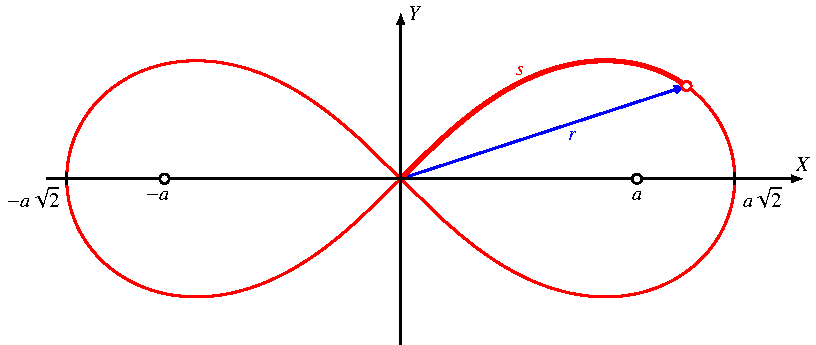
\includegraphics{chapters/110-elliptisch/images/lemniskate.pdf}
\caption{Bogenlänge und Radius der Lemniskate von Bernoulli.
\label{buch:elliptisch:fig:lemniskate}}
\end{figure}
Die Lemniskate von Bernoulli ist die Kurve vierten Grades mit der Gleichung
\begin{equation}
(X^2+Y^2)^2 = 2a^2(X^2-Y^2).
\label{buch:elliptisch:eqn:lemniskate}
\end{equation}
Sie ist in Abbildung~\ref{buch:elliptisch:fig:lemniskate}
dargestellt.
Die beiden Scheitel der Lemniskate befinden sich bei $X_s=\pm a\sqrt{2}$.
Dividiert man die Gleichung der Lemniskate durch $X_s^2=4a^4$ entsteht 
\begin{equation}
\biggl(
\biggl(\frac{X}{a\sqrt{2}}\biggr)^2
+
\biggl(\frac{Y}{a\sqrt{2}}\biggr)^2
\biggr)^2
=
2\frac{a^2}{2a^2}\biggl(
\biggl(\frac{X}{a\sqrt{2}}\biggr)^2
-
\biggl(\frac{Y}{a\sqrt{2}}\biggr)^2
\biggr).
\qquad
\Leftrightarrow
\qquad
(x^2+y^2)^2 = x^2-y^2,
\label{buch:elliptisch:eqn:lemniskatenormiert}
\end{equation}
wobei wir $x=X/a\sqrt{2}$ und $y=Y/a\sqrt{2}$ gesetzt haben.
In dieser Normierung liegen die Scheitel bei $\pm 1$.
Dies ist die Skalierung, die für die Definition des lemniskatischen
Sinus und Kosinus verwendet werden soll.

In Polarkoordinaten $x=r\cos\varphi$ und $y=r\sin\varphi$
gilt nach Einsetzen in \eqref{buch:elliptisch:eqn:lemniskatenormiert}
\begin{equation}
r^4
=
r^2(\cos^2\varphi-\sin^2\varphi)
=
r^2\cos2\varphi
\qquad\Rightarrow\qquad
r^2 = \cos 2\varphi
\label{buch:elliptisch:eqn:lemniskatepolar}
\end{equation}
als Darstellung der Lemniskate in Polardarstellung.
Sie gilt für Winkel $\varphi\in[-\frac{\pi}4,\frac{\pi}4]$ für das
rechte Blatt und $\varphi\in[\frac{3\pi}4,\frac{5\pi}4]$ für das linke
Blatt der Lemniskate.

\subsection{Bogenlänge}
Die Funktionen
\begin{equation}
x(r) = \frac{r}{\sqrt{2}}\sqrt{1+r^2},
\quad
y(r) = \frac{r}{\sqrt{2}}\sqrt{1-r^2}
\label{buch:geometrie:eqn:lemniskateparam}
\end{equation}
erfüllen
\begin{align*}
x(r)^2-y(r)^2
&=
\frac{r^2(1+r^2)}{2}-\frac{r^2(1-r^2)}{2}
\\
&
=
r^4
=
(x(r)^2 + y(r)^2)^2,
\end{align*}
sie stellen also eine Parametrisierung der Lemniskate dar.

Mit Hilfe der Parametrisierung~\eqref{buch:geometrie:eqn:lemniskateparam}
kann man die Länge $s$ des in Abbildung~\ref{buch:elliptisch:fig:lemniskate}
dargestellten Bogens der Lemniskate berechnen.
Dazu benötigt man die Ableitungen nach $r$, die man mit der Produkt- und
Kettenregel berechnen kann:
\begin{align*}
\dot{x}(r)
&=
\frac{\sqrt{1+r^2}}{\sqrt{2}}
+
\frac{r^2}{\sqrt{2}\sqrt{1+r^2}}
&&\Rightarrow&
\dot{x}(r)^2
&=
\frac{1+r^2}{2} +r^2 + \frac{r^4}{2(1+r^2)}
\\
\dot{y}(r)
&=
\frac{\sqrt{1-r^2}}{\sqrt{2}}
-
\frac{r^2}{\sqrt{2}\sqrt{1-r^2}}
&&\Rightarrow&
\dot{y}(r)^2
&=
\frac{1-r^2}{2} -r^2 + \frac{r^4}{2(1-r^2)}
\end{align*}
Die Summe der Quadrate ist
\begin{align*}
\dot{x}(r)^2 + \dot{y}(r)^2
&=
1 + r^4\frac{1-r^2+1+r^2}{2(1+r^2)(1-r^2)}
=
1+r^4\frac{2}{2(1-r^4)}
=
\frac{1-r^4+r^4}{1-r^4}
=
\frac1{1-r^4}.
\end{align*}
Durch Einsetzen in das Integral für die Bogenlänge bekommt man
\begin{equation}
s(r)
=
\int_0^r
\frac{1}{\sqrt{1-t^4}}\,dt.
\label{buch:elliptisch:eqn:lemniskatebogenlaenge}
\end{equation}

%
% Als elliptisches Integral
%
\subsection{Darstellung als elliptisches Integral}
Das unvollständige elliptische Integral erster Art mit Parameter
$k^2=-1$ oder $k=i$ ist
\[
K(r,i)
=
\int_0^x \frac{dt}{\sqrt{(1-t^2)(1-i^2 t^2)}}
=
\int_0^x \frac{dt}{\sqrt{(1-t^2)(1-(-1)t^2)}}
=
\int_0^x \frac{dt}{\sqrt{1-t^4}}
=
s(r).
\]
Der lemniskatische Sinus ist also eine Umkehrfunktion des
elliptischen Integrals erster Art für den speziellen Wert $i$ des
Parameters $k$.

Die Länge des rechten Blattes der Lemniskate wird mit $\varpi$ bezeichnet
und hat den numerischen Wert
\[
\varpi
=
2\int_0^1\sqrt{\frac{1}{1-t^4}}\,dt
=
2.6220575542.
\]
$\varpi$ ist auch als die {\em lemniskatische Konstante} bekannt.
\index{lemniskatische Konstante}%
Der Lemniskatenbogen zwischen dem Nullpunkt und $(1,0)$ hat die Länge
$\varpi/2$.

%
%  Bogenlängenparametrisierung
%
\subsection{Bogenlängenparametrisierung}
Die Lemniskate mit der Gleichung
\[
(X^2+X^2)^2=2(X^2-X^2)
\]
(der Fall $a=1$ in \eqref{buch:elliptisch:eqn:lemniskate})
kann mit Jacobischen elliptischen Funktionen
parametrisiert werden.
Dazu schreibt man
\[
\left.
\begin{aligned}
X(t)
&=
\sqrt{2}\operatorname{cn}(t,k) \operatorname{dn}(t,k)
\\
Y(t)
&=
\phantom{\sqrt{2}}
\operatorname{cn}(t,k) \operatorname{sn}(t,k)
\end{aligned}
\quad\right\}
\qquad\text{mit $k=\displaystyle\frac{1}{\sqrt{2}}$}
\]
und berechnet die beiden Seiten der definierenden Gleichung der
Lemniskate.
Zunächst ist
\begin{align*}
X(t)^2
&=
2\operatorname{cn}(t,k)^2
\operatorname{dn}(t,k)^2
\\
Y(t)^2
&=
\operatorname{cn}(t,k)^2
\operatorname{sn}(t,k)^2
\\
X(t)^2+Y(t)^2
&=
2\operatorname{cn}(t,k)^2
\bigl(
\underbrace{
\operatorname{dn}(t,k)^2
+{\textstyle\frac12}
\operatorname{sn}(t,k)^2
}_{\displaystyle =1}
\bigr)
%\\
%&
=
2\operatorname{cn}(t,k)^2
\\
X(t)^2-Y(t)^2
&=
\operatorname{cn}(t,k)^2
\bigl(
2\operatorname{dn}(t,k)^2 - \operatorname{sn}(t,k)^2
\bigr)
\\
&=
\operatorname{cn}(t,k)^2
\bigl(
2\bigl({\textstyle\frac12}+{\textstyle\frac12}\operatorname{cn}(t,k)^2\bigr)
-
\bigl(1-\operatorname{cn}(t,k)^2\bigr)
\bigr)
\\
&=
2\operatorname{cn}(t,k)^4
\\
\Rightarrow\qquad
(X(t)^2+Y(t)^2)^2
&=
4\operatorname{cn}(t,k)^4
=
2(X(t)^2-Y(t)^2).
\end{align*}
Wir zeigen jetzt, dass dies tatsächlich eine Bogenlängenparametrisierung
der Lemniskate ist.
Dazu berechnen wir die Ableitungen
\begin{align*}
\dot{X}(t)
&=
\sqrt{2}\operatorname{cn}'(t,k)\operatorname{dn}(t,k)
+
\sqrt{2}\operatorname{cn}(t,k)\operatorname{dn}'(t,k)
\\
&=
-\sqrt{2}\operatorname{sn}(t,k)\operatorname{dn}(t,k)^2
-\frac12\sqrt{2}\operatorname{sn}(t,k)\operatorname{cn}(t,k)^2
\\
&=
-\sqrt{2}\operatorname{sn}(t,k)\bigl(
1-{\textstyle\frac12}\operatorname{sn}(t,k)^2
+{\textstyle\frac12}-{\textstyle\frac12}\operatorname{sn}(u,t)^2
\bigr)
\\
&=
\sqrt{2}\operatorname{sn}(t,k)
\bigl(
{\textstyle \frac32}-\operatorname{sn}(t,k)^2
\bigr)
\\
\dot{X}(t)^2
&=
2\operatorname{sn}(t,k)^2
\bigl(
{\textstyle \frac32}-\operatorname{sn}(t,k)^2
\bigr)^2
\\
&=
{\textstyle\frac{9}{2}}\operatorname{sn}(t,k)^2
-
6\operatorname{sn}(t,k)^4
+2\operatorname{sn}(t,k)^6
\\
\dot{Y}(t)
&=
\operatorname{cn}'(t,k)\operatorname{sn}(t,k)
+
\operatorname{cn}(t,k)\operatorname{sn}'(t,k)
\\
&=
-\operatorname{sn}(t,k)^2
\operatorname{dn}(t,k)
+\operatorname{cn}(t,k)^2
\operatorname{dn}(t,k)
\\
&=
\operatorname{dn}(t,k)\bigl(1-2\operatorname{sn}(t,k)^2\bigr)
\\
\dot{Y}(t)^2
&=
\bigl(1-{\textstyle\frac12}\operatorname{sn}(t,k)^2\bigr)
\bigl(1-2\operatorname|{sn}(t,k)^2\bigr)^2
\\
&=
1-{\textstyle\frac{9}{2}}\operatorname{sn}(t,k)^2
+6\operatorname{sn}(t,k)^4
-2\operatorname{sn}(t,k)^6
\\
\dot{X}(t)^2 + \dot{Y}(t)^2
&=
1.
\end{align*}
Dies bedeutet, dass die Bogenlänge zwischen den Parameterwerten $0$ und $s$
\[
\int_0^s
\sqrt{\dot{X}(t)^2 + \dot{Y}(t)^2}
\,dt
=
\int_0^s\,dt
=
s,
\]
der Parameter $t$ ist also ein Bogenlängenparameter.

Die mit dem Faktor $1/\sqrt{2}$ skalierte Standard-Lemniskate mit der
Gleichung
\[
(x^2+y^2)^2 = x^2-y^2
\]
hat daher eine Bogenlängenparametrisierung mit
\begin{equation}
\begin{aligned}
x(t)
&=
\phantom{\frac{1}{\sqrt{2}}}
\operatorname{cn}(\sqrt{2}t,k)\operatorname{dn}(\sqrt{2}t,k)
\\
y(t)
&=
\frac{1}{\sqrt{2}}\operatorname{cn}(\sqrt{2}t,k)\operatorname{sn}(\sqrt{2}t,k)
\end{aligned}
\label{buch:elliptisch:lemniskate:bogenlaenge}
\end{equation}

\subsection{Der lemniskatische Sinus und Kosinus}
Der Sinus Berechnet die Gegenkathete zu einer gegebenen Bogenlänge des
Kreises, er ist die Umkehrfunktion der Funktion, die der Gegenkathete
die Bogenlänge zuordnet.

Daher ist es naheliegend, die Umkehrfunktion von $s(r)$ in 
\eqref{buch:elliptisch:eqn:lemniskatebogenlaenge}
den {\em lemniskatischen Sinus} zu nennen mit der Bezeichnung
$r=\operatorname{sl} s$.

Der Kosinus ist der Sinus des komplementären Winkels.
Auch für die lemniskatische Bogenlänge $s(r)$ lässt sich eine
komplementäre Bogenlänge definieren, nämlich die Bogenlänge zwischen
dem Punkt $(x(r), y(r))$ und $(1,0)$.

Da die Parametrisierung~\eqref{buch:elliptisch:lemniskate:bogenlaenge}
eine Bogenlängenparametrisierung ist, darf man $t=s$ schreiben.
Dann kann man aber auch $r(s)$ daraus berechnen,
es ist
\[
r(s)^2
=
x(s)^2 + y(s)^2
=
\operatorname{cn}(s\sqrt{2},k)^2
\qquad\Rightarrow\qquad
r(s)
=
\operatorname{cn}(s\sqrt{2},k)
\]

\begin{figure}
\centering
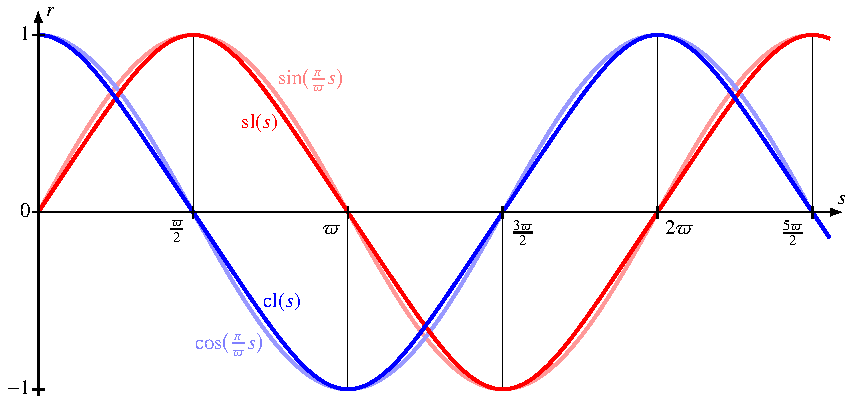
\includegraphics{chapters/110-elliptisch/images/slcl.pdf}
\caption{
Lemniskatischer Sinus und Kosinus sowie Sinus und Kosinus
mit derart skaliertem Argument, dass die Funktionen die gleichen Nullstellen
haben.
\label{buch:elliptisch:figure:slcl}}
\end{figure}


%\section*{Übungsaufgaben}
%\rhead{Übungsaufgaben}
%\aufgabetoplevel{chapters/020-exponential/uebungsaufgaben}
%\begin{uebungsaufgaben}
%\uebungsaufgabe{0}
%\uebungsaufgabe{1}
%\end{uebungsaufgaben}


% Gamma und Pi

% Spezielle Funktionenfamilien
%%
% chapter.tex -- Beschreibung des Inhaltes
%
% (c) 2021 Prof Dr Andreas Müller, Hochschule Rapperswil
%
% !TeX spellcheck = de_CH
\chapter{Elliptische Funktionen
\label{buch:chapter:geometrie}}
\lhead{Elliptische Funktionen}
\rhead{}

Der Versuch, die Länge eines Ellipsenbogens zu berechnen, hat
in Abschnitt~\ref{buch:geometrie:subsection:hyperbeln-und-ellipsen}
zu Integralen geführt, die nicht in geschlossener Form ausgewertet
werden können.
Neben den dort gefundenen Integralen sind noch weitere, ähnlich
aufgebaute Integrale in dieser Familie zu finden.

%
% ellintegral.tex
%
% (c) 2021 Prof Dr Andreas Müller, OST Ostschweizer Fachhochschule
%
\section{Elliptische Integrale
\label{buch:elliptisch:section:integral}}
\rhead{Elliptisches Integral}
Bei der Berechnung des Ellipsenbogens in 
Abschnitt~\ref{buch:geometrie:subsection:hyperbeln-und-ellipsen}
sind wir auf ein Integral gestossen, welches sich nicht in geschlossener
Form ausdrücken liess.
Um solche Integrale in den Griff zu bekommen, ist es nötig, sie als
neue spezielle Funktionen zu definieren.

\subsection{Definition
\label{buch:elliptisch:subsection:definition}}
Ein {\em elliptisches Integral} ist ein Integral der Form
\index{elliptishes Integral}%
\index{Integral, elliptisch}%
\begin{equation}
\int R\left( x, \sqrt{p(x)}\right)\,dx
\label{buch:elliptisch:def:allgemein}
\end{equation}
wobei $R(x,y)$ eine rationale Funktion von zwei Variablen ist und
$p(x)$ ein Polynom dritten oder vierten Grades.
Hätte $p(x)$ ein mehrfache Nullstelle $x_0$, müsste es durch $(x-x_0)^2$
teilbar sein, man könnte also einen Faktor $(x-x_0)$ aus der
Wurzel im Integraneden von \eqref{buch:elliptisch:def:allgemein}
ausklammern und damit das Integral in eine Form bringen, wo $p(x)$
höchstens zweiten Grades ist.
Solche Integrale lassen sich meistens mit trigonometrischen Substitutionen
berechnen.
Wir verlangen daher, dass $p(x)$ keine mehrfachen Nullstellen hat.

Man kann zeigen, dass sich elliptische Integrale in Summen von
elementaren Funktionen und speziellen elliptischen Integralen 
der folgenden Form überführen lassen
\cite[Abschnitt 164, p.~506]{buch:smirnov32}.

\begin{definition}
\label{buch:elliptisch:def:integrale123}
Die elliptischen Integrale erster, zweiter und dritter Art sind die
Integrale
\[
\begin{aligned}
\text{1.~Art:}&&&
\int \frac{dx}{\sqrt{(1-x^2)(1-k^2x^2)}}
\\
\text{2.~Art:}&&&
\int \sqrt{\frac{1-k^2x^2}{1-x^2}}\,dx
\\
\text{3.~Art:}&&&
\int \frac{dx}{(1-nx^2)\sqrt{(1-x^2)(1-k^2x^2)}}
\end{aligned}
\]
mit $0<k<1$.
Es ist auch üblich, den Parameter $m=k^2$ zu verwenden.
\end{definition}

Wie gesagt lassen sich für diese unbestimmten Integrale keine 
geschlossenen Formen finden.
Es bleibt uns daher nichts anderes übrig, als die Integralgrenzen
festzulegen und damit eine Stammfunktion auszuwählen.

%
% Elliptisches Integral
%
\subsection{Vollständige elliptische Integrale
\label{buch:elliptisch:subsection:vollstaendig}}
In diesem Abschnitt legen wir beide Integrationsgrenzen fest und
untersuchen die entstehenenden Funktionen von den Parametern
$k$ und $n$.

\subsubsection{Definition der vollständigen elliptischen Integrale}
Da der Nenner in allen drei elliptischen Integralen eine Nullstelle
bei $\pm1$ hat, kann das Integral nur von $0$ bis $1$ erstreckt werden.

\begin{definition}
\label{buch:elliptisch:def:vollstintegrale123}
Die vollständigen elliptischen Integrale erster, zweiter und dritter
Art sind
\[
\begin{aligned}
\text{1.~Art:}&&
K(k)&=\int_0^1 \frac{dt}{\sqrt{(1-t^2)(1-k^2t^2)}} \\
\text{2.~Art:}&&
E(k)&=\int_0^1 \sqrt{\frac{1-k^2t^2}{1-t^2}}\,dt \\
\text{3.~Art:}&&
\Pi(n, k)&=\int_0^1\frac{dt}{(1-nt^2)\sqrt{(1-t^2)(1-k^2t^2)}} 
\end{aligned}
\]
mit $0<k<1$.
\end{definition}

Die Funktionen hängen stetig von $k$ ab.
Die Nullstellen des Faktors $1-k^2x^2$ liegen ausserhalb des
Integrationsintervalls und spielen daher keine Rolle.
Die Werte von $K(k)$ und $E(k)$ für $k=0$ können direkt berechnet
werden:
\begin{align*}
K(0)
=
E(0)
&=
\int_0^1 \frac{dt}{\sqrt{1-t^2}}=\frac{\pi}2.
\end{align*}
Das Integral $\Pi(n,0)$ ist etwas komplizierter.

Für $k\to 1$ ist $E(k)=1$, die Integrale $K(1)$ und $\Pi(n,1)$
sind dagegen divergent.

\subsubsection{Jacobi- und Legendre-Normalform}
Die Integrationsvariable $t$ der vollständigen elliptischen Integrale
kann durch die Substitution $t=\sin\varphi$ durch die Variable
$\varphi$ und das Integral über das Intervall $[0,1]$ durch ein
Integral über das Intervall $[0,\frac{\pi}2]$ ersetzt werden.
Mit
\[
\frac{dt}{d\varphi} = \cos\varphi = \sqrt{1-\sin^2\varphi}
\]
können die Funktionen $K(k)$, $E(k)$ und $\Pi(n,k)$ auch als
\begin{align*}
K(k)
&=
\int_0^{\frac{\pi}2}
\frac{
\sqrt{1-\sin^2\varphi}\,d\varphi
}{
\sqrt{(1-\sin^2\varphi)(1-k^2\sin^2\varphi)}
}
=
\int_0^{\frac{\pi}2}
\frac{d\varphi}{\sqrt{1-k^2\sin^2\varphi}}
\\
E(k)
&=
\int_0^{\frac{\pi}2}
\sqrt{\frac{1-k^2\sin^2\varphi}{1-\sin^2\varphi}}\sqrt{1-\sin^2\varphi}\,d\varphi
=
\int_0^{\frac{\pi}2}
\sqrt{1-k^2\sin^2\varphi}\,d\varphi
\\
\Pi(n,k)
&=
\int_0^{\frac{\pi}2}
\frac{
\sqrt{1-\sin^2\varphi}\,d\varphi
}{
(1-n\sin^2\varphi)\sqrt{(1-\sin^2\varphi)(1-k^2\sin^2\varphi)}
}
=
\int_0^{\frac{\pi}2}
\frac{
d\varphi
}{
(1-n\sin^2\varphi)\sqrt{1-k^2\sin^2\varphi}
}
\end{align*}
Diese Form wird auch die {\em Legendre-Normalform} der vollständigen 
\index{Legendre-Normalform}%
elliptischen Integrale genannt, während die Form von
Definition~\ref{buch:elliptisch:def:vollstintegrale123}
die {\em Jacobi-Normalform} heisst.
\index{Jacobi-Normalform}%

\subsubsection{Umfang einer Ellipse}
\begin{figure}
\centering
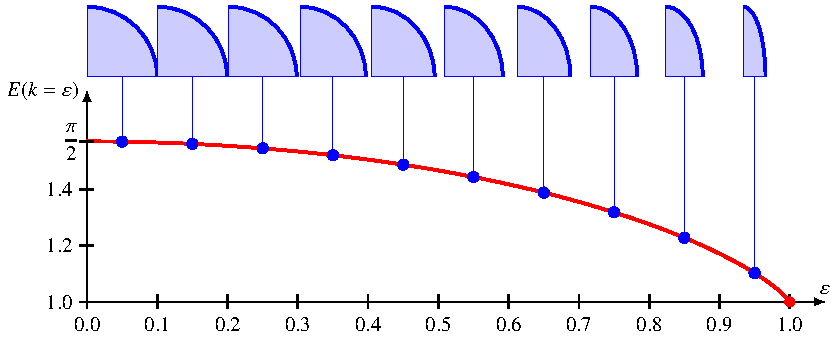
\includegraphics{chapters/110-elliptisch/images/ellipsenumfang.pdf}
\caption{Bogenlänge eines Viertels einer Ellipse mit Exzentrizität
$\varepsilon$.
\label{buch:elliptisch:fig:ellipsenumfang}}
\end{figure}
Wir zeigen, wie sich die Berechnung des Umfangs $U$ einer Ellipse
mit Halbachsen $a$ und $b$, $a\le b$, auf ein volltändiges elliptisches
Integral zurückführen lässt.
Der Fall $a>b$ kann behandelt werden, indem die $x$- und $y$-Koordinaten
vertauscht werden.

Die Parametrisierung
\[
t\mapsto \begin{pmatrix}a\cos t\\ b\sin t\end{pmatrix}
\]
einer Ellipse führt auf das Integral
\begin{align*}
U
&=
\int_0^{2\pi} \sqrt{a^2\sin^2t + b^2\cos^2 t}\,dt
\notag
\\
&=
4\int_0^{\frac{\pi}2}
\sqrt{a^2\sin^2t + b^2(1-\sin^2 t)}
\,dt
\notag
\\
&=
4b \int_0^{\frac{\pi}2} \sqrt{1-(b^2-a^2)/b^2\cdot \sin^2t}\,dt
\label{buch:elliptisch:eqn:umfangellipse}
\end{align*}
für den Umfang der Ellipse.
Bei einem Kreis ist $a=b$ und der zweite Term unter der Wurzel fällt weg,
der Umfang wird $4b\frac{\pi}2=2\pi b$.
Die Differenz $e^2=b^2-a^2$ ist die {\em lineare Exzentrizität} der Ellipse,
\index{lineare Exzentrizität}%
der Quotient $e/b$ wird die {\em numerische Exzentrizität} der Ellipse
genannt.
Insbesondere ist $k = \varepsilon$.

Das Integral~\eqref{buch:elliptisch:eqn:umfangellipse} erhält jetzt die
Form
\[
U
=
4b\int_0^{\frac{\pi}2} \sqrt{1-k^2\sin^2t}\,dt
\]
und ist damit als elliptisches Integral zweiter Art erkannt.
Für den Umfang der Ellipse finden wir damit die Formel
\[
U
=
4b E(k)
=
4b E(\varepsilon).
\]
Das vollständige elliptische Integral zweiter Art $E(\varepsilon)$
liefert also genau den Umfang der eines Viertels Ellipse mit
numerischer Exzentrizität $\varepsilon$ und kleiner Halbachse $1$.

\subsubsection{Komplementäre Integrale}
XXX Komplementäre Integrale \\

\subsubsection{Ableitung}
XXX Ableitung \\
XXX Stammfunktion \\

\subsection{Unvollständige elliptische Integrale}
XXX Vollständige und Unvollständige Integrale \\
XXX Additionstheoreme \\
XXX Parameterkonventionen \\

\subsection{Potenzreihe}
XXX Potenzreihen \\
XXX Als hypergeometrische Funktionen \\



\section{Jacobische elliptische Funktionen}

Für das elliptische Filter werden, wie es der Name bereits deutet, elliptische Funktionen gebraucht.
Wie die trigonometrischen Funktionen Zusammenhänge eines Kreises darlegen, beschreiben die elliptischen Funktionen Ellipsen.
Es ist daher naheliegend, dass der Kosinus des Tschebyscheff-Filters gegen ein elliptisches Pendant ausgetauscht werden könnte.
Der Begriff elliptische Funktion wird für sehr viele Funktionen gebraucht, daher ist es hier wichtig zu erwähnen, dass es ausschliesslich um die Jacobischen elliptischen Funktionen geht.

\subsection{Grundlegende Eigenschaften}

Die Jacobi elliptischen Funktionen werden ausführlich im Kapitel \ref{buch:elliptisch:section:jacobi} behandelt.
Im Wesentlichen erweitern die Jacobi elliptischen Funktionen die trigonometrische Funktionen für Ellipsen.
Zum Beispiel gibt es analog zum Sinus den elliptischen $\sn(z, k)$.
Im Gegensatz zum den trigonometrischen Funktionen haben die elliptischen Funktionen zwei Parameter.
Den \textit{elliptische Modul} $k$, der die Exzentrizität der Ellipse parametrisiert und das Winkelargument $z$.
Im Kreis ist der Radius für alle Winkel konstant, bei Ellipsen ändert sich das.
Dies hat zur Folge, dass bei einer Ellipse die Kreisbogenlänge nicht linear zum Winkel verläuft.
Darum kann hier nicht der gewohnte Winkel verwendet werden.
Das Winkelargument $z$ kann durch das elliptische Integral erster Art
\begin{equation}
    z
    =
    F(\phi, k)
    =
    \int_{0}^{\phi}
    \frac{
        d\theta
    }{
        \sqrt{
            1-k^2 \sin^2 \theta
        }
    }
\end{equation}
mit dem Winkel $\phi$ in Verbindung gebracht werden.

Dabei wird das vollständige und unvollständige elliptische integral unterschieden.
Beim vollständigen Integral
\begin{equation}
    K(k)
    =
    \int_{0}^{\pi / 2}
    \frac{
        d\theta
    }{
        \sqrt{
            1-k^2 \sin^2 \theta
        }
    }
\end{equation}
wird über ein viertel Ellipsenbogen integriert, also bis $\phi=\pi/2$ und liefert das Winkelargument für eine Vierteldrehung.
Die Zahl wird oft auch abgekürzt mit $K = K(k)$ und ist für das elliptische Filter sehr relevant.
Alle elliptischen Funktionen sind somit $4K$-periodisch.

Neben dem $\sn$ gibt es zwei weitere elliptische Basisfunktionen $\cn$ und $\dn$.
Dazu kommen noch weitere abgeleitete Funktionen, die durch Quotienten und Kehrwerte dieser Funktionen zustande kommen.
Insgesamt sind es die zwölf Funktionen
\begin{equation*}
    \sn \quad
    \ns \quad
    \scelliptic \quad
    \sd \quad
    \cn \quad
    \nc \quad
    \cs \quad
    \cd \quad
    \dn \quad
    \nd \quad
    \ds \quad
    \dc.
\end{equation*}

Die Jacobischen elliptischen Funktionen können mit der inversen Funktion des vollständigen elliptischen Integrals erster Art
\begin{equation}
    \phi = F^{-1}(z, k)
\end{equation}
definiert werden. Dabei ist zu beachten dass nur das $z$ Argument der Funktion invertiert wird, also
\begin{equation}
    z = F(\phi, k)
    \Leftrightarrow
    \phi = F^{-1}(z, k).
\end{equation}
Mithilfe von $F^{-1}$ kann zum Beispiel $sn^{-1}$ mit dem elliptischen Integral dargestellt werden:
\begin{equation}
    \sin(\phi)
    =
    \sin \left( F^{-1}(z, k) \right)
    =
    \sn(z, k)
    =
    w.
\end{equation}

% \begin{equation} %TODO remove unnecessary equations
%     \phi
%     =
%      F^{-1}(z, k)
%      =
%      \sin^{-1} \big( \sn (z, k ) \big)
%      =
%     \sin^{-1} ( w )
% \end{equation}

% \begin{equation}
%     F(\phi, k)
%     =
%     z
%     =
%     F( \sin^{-1} \big( \sn (z, k ) \big) , k)
%     =
%     F( \sin^{-1} ( w ), k)
% \end{equation}

% \begin{equation}
%     \sn^{-1}(w, k)
%     =
%     F(\phi, k),
%     \quad
%     \phi = \sin^{-1}(w)
% \end{equation}

\subsection{Die Funktion $\sn^{-1}$}

Beim Tschebyscheff-Filter konnten wir mit Betrachten des Arcuscosinus die Funktionalität erklären.
Für das Elliptische Filter machen wir die gleiche Betrachtung mit der $\sn^{-1}$-Funktion.
Der $\sn^{-1}$ ist durch das elliptische Integral
\begin{align}
    \sn^{-1}(w, k)
        & =
    \int_{0}^{\phi}
    \frac{
        d\theta
    }{
        \sqrt{
            1-k^2 \sin^2 \theta
        }
    },
    \quad
    \phi = \sin^{-1}(w)
    \\
        & =
    \int_{0}^{w}
    \frac{
        dt
    }{
        \sqrt{
            (1-t^2)(1-k^2 t^2)
        }
    }
\end{align}
beschrieben.
Dazu betrachten wir wieder den Integranden
\begin{equation}
    \frac{
        1
    }{
        \sqrt{
            (1-t^2)(1-k^2 t^2)
        }
    }.
\end{equation}
Beim $\cos^{-1}(x)$ haben wir gesehen, dass die analytische Fortsetzung bei $x < -1$ und $x > 1$ rechtwinklig in die komplexen Zahlen wandert.
Wenn man das Gleiche mit $\sn^{-1}(w, k)$ macht, erkennt man zwei interessante Stellen.
Die erste ist die gleiche wie beim $\cos^{-1}(x)$ nämlich bei $t = \pm 1$.
Der erste Term unter der Wurzel wird dann negativ, während der zweite noch positiv ist, da $k \leq 1$.
Ab diesem Punkt knickt die Funktion in die imaginäre Richtung ab.
Bei $t = 1/k$ ist auch der zweite Term negativ und die Funktion verläuft in die negative reelle Richtung.
Abbildung \ref{ellfilter:fig:sn} zeigt den Verlauf der Funktion in der komplexen Ebene.
\begin{figure}
    \centering
    \begin{tikzpicture}[>=stealth', auto, node distance=2cm, scale=1.2]

    \tikzstyle{zero} = [draw, circle, inner sep =0, minimum height=0.15cm]

    \tikzset{pole/.style={cross out, draw=black, minimum size=(0.15cm-\pgflinewidth), inner sep=0pt, outer sep=0pt}}

    \begin{scope}[xscale=0.9, yscale=1.8]

        \draw[gray, ->] (0,-1.5) -- (0,1.5) node[anchor=south]{$\mathrm{Im}~z$};
        \draw[gray, ->] (-5,0) -- (5,0) node[anchor=west]{$\mathrm{Re}~z$};

        \begin{scope}

            \clip(-4.5,-1.25) rectangle (4.5,1.25);

            \fill[yellow!30] (0,0) rectangle (1, 0.5);

            \begin{scope}[xshift=-1cm]

                \foreach \i in {-2,...,2} {
                    \foreach \j in {-2,...,1} {
                        \begin{scope}[xshift=\i*4cm, yshift=\j*1cm]
                            \draw[<-, blue!50] (0, 0) -- (0,0.5);
                            \draw[<-, cyan!50] (1, 0) -- (0,0);
                            \draw[<-, darkgreen!50] (2, 0) -- (1,0);
                            \draw[<-, orange!50] (2,0.5) -- (2, 0);
                            \draw[<-, red!50] (1, 0.5) -- (2,0.5);
                            \draw[<-, purple!50] (0, 0.5) -- (1,0.5);
                            \draw[<-, blue!50] (0,1) -- (0,0.5);
                            \draw[<-, orange!50] (2,0.5) -- (2, 1);
                            \draw[<-, red!50] (3, 0.5) -- (2,0.5);
                            \draw[<-, purple!50] (4, 0.5) -- (3,0.5);
                            \draw[<-, darkgreen!50] (2, 0) -- (3,0);
                            \draw[<-, cyan!50] (3, 0) -- (4,0);
                        \end{scope}
                    }
                }

                % \pause
                \draw[ultra thick, <-, darkgreen] (2, 0) -- (1,0);
                % \pause
                \draw[ultra thick, <-, orange] (2,0.5) -- (2, 0);
                % \pause
                \draw[ultra thick, <-, red] (1, 0.5) -- (2,0.5);
                % \pause
                \draw[ultra thick, <-, blue] (0, 0) -- (0,0.5);
                \draw[ultra thick, <-, purple] (0, 0.5) -- (1,0.5);
                \draw[ultra thick, <-, cyan] (1, 0) -- (0,0);
                % \pause


                \foreach \i in {-2,...,2} {
                    \foreach \j in {-2,...,1} {
                        \begin{scope}[xshift=\i*4cm, yshift=\j*1cm]
                            \node[zero] at ( 1, 0) {};
                            \node[zero] at ( 3, 0) {};
                            \node[pole] at ( 1,0.5) {};
                            \node[pole] at ( 3,0.5) {};
                        \end{scope}
                    }
                }

            \end{scope}

        \end{scope}

        \draw[gray] ( 1,0) +(0,0.1) -- +(0, -0.1) node[inner sep=0, anchor=north] {\small $K$};
        \draw[gray]  (0, 0.5) +(0.1, 0) -- +(-0.1, 0) node[inner sep=0, anchor=east]{\small $jK^\prime$};

    \end{scope}

    \node[zero] at (4,3) (n) {};
    \node[anchor=west] at (n.east) {Zero};
    \node[pole, below=0.25cm of n] (n) {};
    \node[anchor=west] at (n.east) {Pole};

    \begin{scope}[yshift=-4cm, xscale=0.75]

        \draw[gray, ->] (-6,0) -- (6,0) node[anchor=west]{$w$};

        \draw[ultra thick, ->, purple] (-5, 0) -- (-3, 0);
        \draw[ultra thick, ->, blue]      (-3, 0) -- (-2, 0);
        \draw[ultra thick, ->, cyan]       (-2, 0) -- (0, 0);
        \draw[ultra thick, ->, darkgreen]    (0, 0) -- (2, 0);
        \draw[ultra thick, ->, orange] (2, 0) -- (3, 0);
        \draw[ultra thick, ->, red] (3, 0) -- (5, 0);

        \node[anchor=south] at (-5,0) {$-\infty$};
        \node[anchor=south] at (-3,0) {$-1/k$};
        \node[anchor=south] at (-2,0) {$-1$};
        \node[anchor=south] at (0,0) {$0$};
        \node[anchor=south] at (2,0) {$1$};
        \node[anchor=south] at (3,0) {$1/k$};
        \node[anchor=south] at (5,0) {$\infty$};

    \end{scope}


\end{tikzpicture}
    \caption{
        $z$-Ebene der Funktion $z = \sn^{-1}(w, k)$.
        Die Funktion ist in der realen Achse $4K$-periodisch und in der imaginären Achse $2jK^\prime$-periodisch.
    }
    \label{ellfilter:fig:sn}
\end{figure}
In der reellen Richtung ist sie $4K(k)$-periodisch und in der imaginären Richtung $4K^\prime(k)$-periodisch, wobei $K^\prime$ das komplementäre vollständige Elliptische Integral ist:
\begin{equation}
    K^\prime(k)
    =
    \int_{0}^{\pi / 2}
    \frac{
        d\theta
    }{
        \sqrt{
            1-{k^\prime}^2 \sin^2 \theta
        }
    },
    \quad
    k^\prime = \sqrt{1-k^2}.
\end{equation}

%
% lemniskate.tex
%
% (c) 2021 Prof Dr Andreas Müller, OST Ostschweizer Fachhochschule
%
\section{Lemniskatischer Sinus
\label{buch:elliptisch:section:lemniskate}}
\rhead{Lemniskatischer Sinus}
Historisch war der {\em lemniskatische Sinus} die erste ellptische
Funktion, die Gauss bereits als 19-jähriger untersucht, aber nicht 
veröffentlich hat.
In diesem Abschnitt soll die Verbindung zu den Jacobischen
elliptischen Funktionen hergestellt werden.

\subsection{Lemniskate
\label{buch:gemotrie:subsection:lemniskate}}
\begin{figure}
\centering
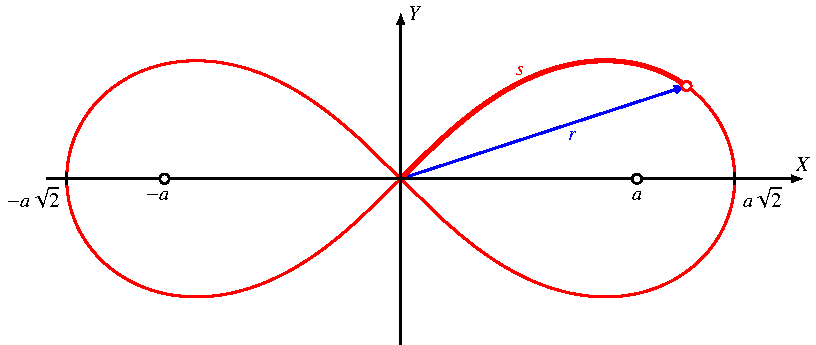
\includegraphics{chapters/110-elliptisch/images/lemniskate.pdf}
\caption{Bogenlänge und Radius der Lemniskate von Bernoulli.
\label{buch:elliptisch:fig:lemniskate}}
\end{figure}
Die Lemniskate von Bernoulli ist die Kurve vierten Grades mit der Gleichung
\begin{equation}
(X^2+Y^2)^2 = 2a^2(X^2-Y^2).
\label{buch:elliptisch:eqn:lemniskate}
\end{equation}
Sie ist in Abbildung~\ref{buch:elliptisch:fig:lemniskate}
dargestellt.
Die beiden Scheitel der Lemniskate befinden sich bei $X_s=\pm a\sqrt{2}$.
Dividiert man die Gleichung der Lemniskate durch $X_s^2=4a^4$ entsteht 
\begin{equation}
\biggl(
\biggl(\frac{X}{a\sqrt{2}}\biggr)^2
+
\biggl(\frac{Y}{a\sqrt{2}}\biggr)^2
\biggr)^2
=
2\frac{a^2}{2a^2}\biggl(
\biggl(\frac{X}{a\sqrt{2}}\biggr)^2
-
\biggl(\frac{Y}{a\sqrt{2}}\biggr)^2
\biggr).
\qquad
\Leftrightarrow
\qquad
(x^2+y^2)^2 = x^2-y^2,
\label{buch:elliptisch:eqn:lemniskatenormiert}
\end{equation}
wobei wir $x=X/a\sqrt{2}$ und $y=Y/a\sqrt{2}$ gesetzt haben.
In dieser Normierung liegen die Scheitel bei $\pm 1$.
Dies ist die Skalierung, die für die Definition des lemniskatischen
Sinus und Kosinus verwendet werden soll.

In Polarkoordinaten $x=r\cos\varphi$ und $y=r\sin\varphi$
gilt nach Einsetzen in \eqref{buch:elliptisch:eqn:lemniskatenormiert}
\begin{equation}
r^4
=
r^2(\cos^2\varphi-\sin^2\varphi)
=
r^2\cos2\varphi
\qquad\Rightarrow\qquad
r^2 = \cos 2\varphi
\label{buch:elliptisch:eqn:lemniskatepolar}
\end{equation}
als Darstellung der Lemniskate in Polardarstellung.
Sie gilt für Winkel $\varphi\in[-\frac{\pi}4,\frac{\pi}4]$ für das
rechte Blatt und $\varphi\in[\frac{3\pi}4,\frac{5\pi}4]$ für das linke
Blatt der Lemniskate.

\subsection{Bogenlänge}
Die Funktionen
\begin{equation}
x(r) = \frac{r}{\sqrt{2}}\sqrt{1+r^2},
\quad
y(r) = \frac{r}{\sqrt{2}}\sqrt{1-r^2}
\label{buch:geometrie:eqn:lemniskateparam}
\end{equation}
erfüllen
\begin{align*}
x(r)^2-y(r)^2
&=
\frac{r^2(1+r^2)}{2}-\frac{r^2(1-r^2)}{2}
\\
&
=
r^4
=
(x(r)^2 + y(r)^2)^2,
\end{align*}
sie stellen also eine Parametrisierung der Lemniskate dar.

Mit Hilfe der Parametrisierung~\eqref{buch:geometrie:eqn:lemniskateparam}
kann man die Länge $s$ des in Abbildung~\ref{buch:elliptisch:fig:lemniskate}
dargestellten Bogens der Lemniskate berechnen.
Dazu benötigt man die Ableitungen nach $r$, die man mit der Produkt- und
Kettenregel berechnen kann:
\begin{align*}
\dot{x}(r)
&=
\frac{\sqrt{1+r^2}}{\sqrt{2}}
+
\frac{r^2}{\sqrt{2}\sqrt{1+r^2}}
&&\Rightarrow&
\dot{x}(r)^2
&=
\frac{1+r^2}{2} +r^2 + \frac{r^4}{2(1+r^2)}
\\
\dot{y}(r)
&=
\frac{\sqrt{1-r^2}}{\sqrt{2}}
-
\frac{r^2}{\sqrt{2}\sqrt{1-r^2}}
&&\Rightarrow&
\dot{y}(r)^2
&=
\frac{1-r^2}{2} -r^2 + \frac{r^4}{2(1-r^2)}
\end{align*}
Die Summe der Quadrate ist
\begin{align*}
\dot{x}(r)^2 + \dot{y}(r)^2
&=
1 + r^4\frac{1-r^2+1+r^2}{2(1+r^2)(1-r^2)}
=
1+r^4\frac{2}{2(1-r^4)}
=
\frac{1-r^4+r^4}{1-r^4}
=
\frac1{1-r^4}.
\end{align*}
Durch Einsetzen in das Integral für die Bogenlänge bekommt man
\begin{equation}
s(r)
=
\int_0^r
\frac{1}{\sqrt{1-t^4}}\,dt.
\label{buch:elliptisch:eqn:lemniskatebogenlaenge}
\end{equation}

%
% Als elliptisches Integral
%
\subsection{Darstellung als elliptisches Integral}
Das unvollständige elliptische Integral erster Art mit Parameter
$k^2=-1$ oder $k=i$ ist
\[
K(r,i)
=
\int_0^x \frac{dt}{\sqrt{(1-t^2)(1-i^2 t^2)}}
=
\int_0^x \frac{dt}{\sqrt{(1-t^2)(1-(-1)t^2)}}
=
\int_0^x \frac{dt}{\sqrt{1-t^4}}
=
s(r).
\]
Der lemniskatische Sinus ist also eine Umkehrfunktion des
elliptischen Integrals erster Art für den speziellen Wert $i$ des
Parameters $k$.

Die Länge des rechten Blattes der Lemniskate wird mit $\varpi$ bezeichnet
und hat den numerischen Wert
\[
\varpi
=
2\int_0^1\sqrt{\frac{1}{1-t^4}}\,dt
=
2.6220575542.
\]
$\varpi$ ist auch als die {\em lemniskatische Konstante} bekannt.
\index{lemniskatische Konstante}%
Der Lemniskatenbogen zwischen dem Nullpunkt und $(1,0)$ hat die Länge
$\varpi/2$.

%
%  Bogenlängenparametrisierung
%
\subsection{Bogenlängenparametrisierung}
Die Lemniskate mit der Gleichung
\[
(X^2+X^2)^2=2(X^2-X^2)
\]
(der Fall $a=1$ in \eqref{buch:elliptisch:eqn:lemniskate})
kann mit Jacobischen elliptischen Funktionen
parametrisiert werden.
Dazu schreibt man
\[
\left.
\begin{aligned}
X(t)
&=
\sqrt{2}\operatorname{cn}(t,k) \operatorname{dn}(t,k)
\\
Y(t)
&=
\phantom{\sqrt{2}}
\operatorname{cn}(t,k) \operatorname{sn}(t,k)
\end{aligned}
\quad\right\}
\qquad\text{mit $k=\displaystyle\frac{1}{\sqrt{2}}$}
\]
und berechnet die beiden Seiten der definierenden Gleichung der
Lemniskate.
Zunächst ist
\begin{align*}
X(t)^2
&=
2\operatorname{cn}(t,k)^2
\operatorname{dn}(t,k)^2
\\
Y(t)^2
&=
\operatorname{cn}(t,k)^2
\operatorname{sn}(t,k)^2
\\
X(t)^2+Y(t)^2
&=
2\operatorname{cn}(t,k)^2
\bigl(
\underbrace{
\operatorname{dn}(t,k)^2
+{\textstyle\frac12}
\operatorname{sn}(t,k)^2
}_{\displaystyle =1}
\bigr)
%\\
%&
=
2\operatorname{cn}(t,k)^2
\\
X(t)^2-Y(t)^2
&=
\operatorname{cn}(t,k)^2
\bigl(
2\operatorname{dn}(t,k)^2 - \operatorname{sn}(t,k)^2
\bigr)
\\
&=
\operatorname{cn}(t,k)^2
\bigl(
2\bigl({\textstyle\frac12}+{\textstyle\frac12}\operatorname{cn}(t,k)^2\bigr)
-
\bigl(1-\operatorname{cn}(t,k)^2\bigr)
\bigr)
\\
&=
2\operatorname{cn}(t,k)^4
\\
\Rightarrow\qquad
(X(t)^2+Y(t)^2)^2
&=
4\operatorname{cn}(t,k)^4
=
2(X(t)^2-Y(t)^2).
\end{align*}
Wir zeigen jetzt, dass dies tatsächlich eine Bogenlängenparametrisierung
der Lemniskate ist.
Dazu berechnen wir die Ableitungen
\begin{align*}
\dot{X}(t)
&=
\sqrt{2}\operatorname{cn}'(t,k)\operatorname{dn}(t,k)
+
\sqrt{2}\operatorname{cn}(t,k)\operatorname{dn}'(t,k)
\\
&=
-\sqrt{2}\operatorname{sn}(t,k)\operatorname{dn}(t,k)^2
-\frac12\sqrt{2}\operatorname{sn}(t,k)\operatorname{cn}(t,k)^2
\\
&=
-\sqrt{2}\operatorname{sn}(t,k)\bigl(
1-{\textstyle\frac12}\operatorname{sn}(t,k)^2
+{\textstyle\frac12}-{\textstyle\frac12}\operatorname{sn}(u,t)^2
\bigr)
\\
&=
\sqrt{2}\operatorname{sn}(t,k)
\bigl(
{\textstyle \frac32}-\operatorname{sn}(t,k)^2
\bigr)
\\
\dot{X}(t)^2
&=
2\operatorname{sn}(t,k)^2
\bigl(
{\textstyle \frac32}-\operatorname{sn}(t,k)^2
\bigr)^2
\\
&=
{\textstyle\frac{9}{2}}\operatorname{sn}(t,k)^2
-
6\operatorname{sn}(t,k)^4
+2\operatorname{sn}(t,k)^6
\\
\dot{Y}(t)
&=
\operatorname{cn}'(t,k)\operatorname{sn}(t,k)
+
\operatorname{cn}(t,k)\operatorname{sn}'(t,k)
\\
&=
-\operatorname{sn}(t,k)^2
\operatorname{dn}(t,k)
+\operatorname{cn}(t,k)^2
\operatorname{dn}(t,k)
\\
&=
\operatorname{dn}(t,k)\bigl(1-2\operatorname{sn}(t,k)^2\bigr)
\\
\dot{Y}(t)^2
&=
\bigl(1-{\textstyle\frac12}\operatorname{sn}(t,k)^2\bigr)
\bigl(1-2\operatorname|{sn}(t,k)^2\bigr)^2
\\
&=
1-{\textstyle\frac{9}{2}}\operatorname{sn}(t,k)^2
+6\operatorname{sn}(t,k)^4
-2\operatorname{sn}(t,k)^6
\\
\dot{X}(t)^2 + \dot{Y}(t)^2
&=
1.
\end{align*}
Dies bedeutet, dass die Bogenlänge zwischen den Parameterwerten $0$ und $s$
\[
\int_0^s
\sqrt{\dot{X}(t)^2 + \dot{Y}(t)^2}
\,dt
=
\int_0^s\,dt
=
s,
\]
der Parameter $t$ ist also ein Bogenlängenparameter.

Die mit dem Faktor $1/\sqrt{2}$ skalierte Standard-Lemniskate mit der
Gleichung
\[
(x^2+y^2)^2 = x^2-y^2
\]
hat daher eine Bogenlängenparametrisierung mit
\begin{equation}
\begin{aligned}
x(t)
&=
\phantom{\frac{1}{\sqrt{2}}}
\operatorname{cn}(\sqrt{2}t,k)\operatorname{dn}(\sqrt{2}t,k)
\\
y(t)
&=
\frac{1}{\sqrt{2}}\operatorname{cn}(\sqrt{2}t,k)\operatorname{sn}(\sqrt{2}t,k)
\end{aligned}
\label{buch:elliptisch:lemniskate:bogenlaenge}
\end{equation}

\subsection{Der lemniskatische Sinus und Kosinus}
Der Sinus Berechnet die Gegenkathete zu einer gegebenen Bogenlänge des
Kreises, er ist die Umkehrfunktion der Funktion, die der Gegenkathete
die Bogenlänge zuordnet.

Daher ist es naheliegend, die Umkehrfunktion von $s(r)$ in 
\eqref{buch:elliptisch:eqn:lemniskatebogenlaenge}
den {\em lemniskatischen Sinus} zu nennen mit der Bezeichnung
$r=\operatorname{sl} s$.

Der Kosinus ist der Sinus des komplementären Winkels.
Auch für die lemniskatische Bogenlänge $s(r)$ lässt sich eine
komplementäre Bogenlänge definieren, nämlich die Bogenlänge zwischen
dem Punkt $(x(r), y(r))$ und $(1,0)$.

Da die Parametrisierung~\eqref{buch:elliptisch:lemniskate:bogenlaenge}
eine Bogenlängenparametrisierung ist, darf man $t=s$ schreiben.
Dann kann man aber auch $r(s)$ daraus berechnen,
es ist
\[
r(s)^2
=
x(s)^2 + y(s)^2
=
\operatorname{cn}(s\sqrt{2},k)^2
\qquad\Rightarrow\qquad
r(s)
=
\operatorname{cn}(s\sqrt{2},k)
\]

\begin{figure}
\centering
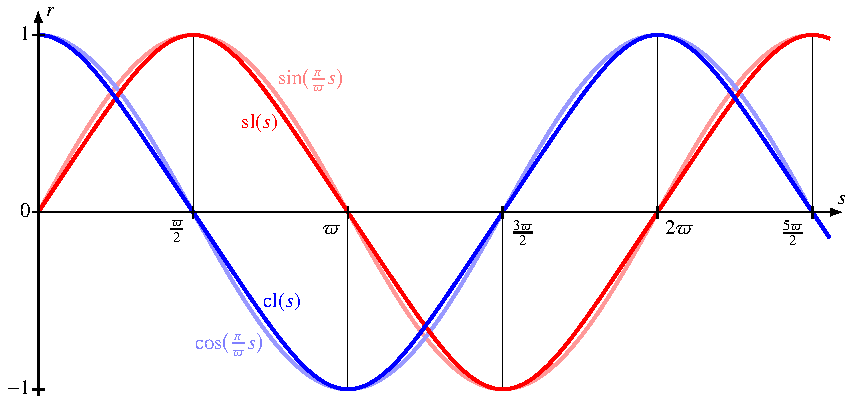
\includegraphics{chapters/110-elliptisch/images/slcl.pdf}
\caption{
Lemniskatischer Sinus und Kosinus sowie Sinus und Kosinus
mit derart skaliertem Argument, dass die Funktionen die gleichen Nullstellen
haben.
\label{buch:elliptisch:figure:slcl}}
\end{figure}


%\section*{Übungsaufgaben}
%\rhead{Übungsaufgaben}
%\aufgabetoplevel{chapters/020-exponential/uebungsaufgaben}
%\begin{uebungsaufgaben}
%\uebungsaufgabe{0}
%\uebungsaufgabe{1}
%\end{uebungsaufgaben}


%
% chapter.tex -- Beschreibung des Inhaltes
%
% (c) 2021 Prof Dr Andreas Müller, Hochschule Rapperswil
%
% !TeX spellcheck = de_CH
\chapter{Elliptische Funktionen
\label{buch:chapter:geometrie}}
\lhead{Elliptische Funktionen}
\rhead{}

Der Versuch, die Länge eines Ellipsenbogens zu berechnen, hat
in Abschnitt~\ref{buch:geometrie:subsection:hyperbeln-und-ellipsen}
zu Integralen geführt, die nicht in geschlossener Form ausgewertet
werden können.
Neben den dort gefundenen Integralen sind noch weitere, ähnlich
aufgebaute Integrale in dieser Familie zu finden.

%
% ellintegral.tex
%
% (c) 2021 Prof Dr Andreas Müller, OST Ostschweizer Fachhochschule
%
\section{Elliptische Integrale
\label{buch:elliptisch:section:integral}}
\rhead{Elliptisches Integral}
Bei der Berechnung des Ellipsenbogens in 
Abschnitt~\ref{buch:geometrie:subsection:hyperbeln-und-ellipsen}
sind wir auf ein Integral gestossen, welches sich nicht in geschlossener
Form ausdrücken liess.
Um solche Integrale in den Griff zu bekommen, ist es nötig, sie als
neue spezielle Funktionen zu definieren.

\subsection{Definition
\label{buch:elliptisch:subsection:definition}}
Ein {\em elliptisches Integral} ist ein Integral der Form
\index{elliptishes Integral}%
\index{Integral, elliptisch}%
\begin{equation}
\int R\left( x, \sqrt{p(x)}\right)\,dx
\label{buch:elliptisch:def:allgemein}
\end{equation}
wobei $R(x,y)$ eine rationale Funktion von zwei Variablen ist und
$p(x)$ ein Polynom dritten oder vierten Grades.
Hätte $p(x)$ ein mehrfache Nullstelle $x_0$, müsste es durch $(x-x_0)^2$
teilbar sein, man könnte also einen Faktor $(x-x_0)$ aus der
Wurzel im Integraneden von \eqref{buch:elliptisch:def:allgemein}
ausklammern und damit das Integral in eine Form bringen, wo $p(x)$
höchstens zweiten Grades ist.
Solche Integrale lassen sich meistens mit trigonometrischen Substitutionen
berechnen.
Wir verlangen daher, dass $p(x)$ keine mehrfachen Nullstellen hat.

Man kann zeigen, dass sich elliptische Integrale in Summen von
elementaren Funktionen und speziellen elliptischen Integralen 
der folgenden Form überführen lassen
\cite[Abschnitt 164, p.~506]{buch:smirnov32}.

\begin{definition}
\label{buch:elliptisch:def:integrale123}
Die elliptischen Integrale erster, zweiter und dritter Art sind die
Integrale
\[
\begin{aligned}
\text{1.~Art:}&&&
\int \frac{dx}{\sqrt{(1-x^2)(1-k^2x^2)}}
\\
\text{2.~Art:}&&&
\int \sqrt{\frac{1-k^2x^2}{1-x^2}}\,dx
\\
\text{3.~Art:}&&&
\int \frac{dx}{(1-nx^2)\sqrt{(1-x^2)(1-k^2x^2)}}
\end{aligned}
\]
mit $0<k<1$.
Es ist auch üblich, den Parameter $m=k^2$ zu verwenden.
\end{definition}

Wie gesagt lassen sich für diese unbestimmten Integrale keine 
geschlossenen Formen finden.
Es bleibt uns daher nichts anderes übrig, als die Integralgrenzen
festzulegen und damit eine Stammfunktion auszuwählen.

%
% Elliptisches Integral
%
\subsection{Vollständige elliptische Integrale
\label{buch:elliptisch:subsection:vollstaendig}}
In diesem Abschnitt legen wir beide Integrationsgrenzen fest und
untersuchen die entstehenenden Funktionen von den Parametern
$k$ und $n$.

\subsubsection{Definition der vollständigen elliptischen Integrale}
Da der Nenner in allen drei elliptischen Integralen eine Nullstelle
bei $\pm1$ hat, kann das Integral nur von $0$ bis $1$ erstreckt werden.

\begin{definition}
\label{buch:elliptisch:def:vollstintegrale123}
Die vollständigen elliptischen Integrale erster, zweiter und dritter
Art sind
\[
\begin{aligned}
\text{1.~Art:}&&
K(k)&=\int_0^1 \frac{dt}{\sqrt{(1-t^2)(1-k^2t^2)}} \\
\text{2.~Art:}&&
E(k)&=\int_0^1 \sqrt{\frac{1-k^2t^2}{1-t^2}}\,dt \\
\text{3.~Art:}&&
\Pi(n, k)&=\int_0^1\frac{dt}{(1-nt^2)\sqrt{(1-t^2)(1-k^2t^2)}} 
\end{aligned}
\]
mit $0<k<1$.
\end{definition}

Die Funktionen hängen stetig von $k$ ab.
Die Nullstellen des Faktors $1-k^2x^2$ liegen ausserhalb des
Integrationsintervalls und spielen daher keine Rolle.
Die Werte von $K(k)$ und $E(k)$ für $k=0$ können direkt berechnet
werden:
\begin{align*}
K(0)
=
E(0)
&=
\int_0^1 \frac{dt}{\sqrt{1-t^2}}=\frac{\pi}2.
\end{align*}
Das Integral $\Pi(n,0)$ ist etwas komplizierter.

Für $k\to 1$ ist $E(k)=1$, die Integrale $K(1)$ und $\Pi(n,1)$
sind dagegen divergent.

\subsubsection{Jacobi- und Legendre-Normalform}
Die Integrationsvariable $t$ der vollständigen elliptischen Integrale
kann durch die Substitution $t=\sin\varphi$ durch die Variable
$\varphi$ und das Integral über das Intervall $[0,1]$ durch ein
Integral über das Intervall $[0,\frac{\pi}2]$ ersetzt werden.
Mit
\[
\frac{dt}{d\varphi} = \cos\varphi = \sqrt{1-\sin^2\varphi}
\]
können die Funktionen $K(k)$, $E(k)$ und $\Pi(n,k)$ auch als
\begin{align*}
K(k)
&=
\int_0^{\frac{\pi}2}
\frac{
\sqrt{1-\sin^2\varphi}\,d\varphi
}{
\sqrt{(1-\sin^2\varphi)(1-k^2\sin^2\varphi)}
}
=
\int_0^{\frac{\pi}2}
\frac{d\varphi}{\sqrt{1-k^2\sin^2\varphi}}
\\
E(k)
&=
\int_0^{\frac{\pi}2}
\sqrt{\frac{1-k^2\sin^2\varphi}{1-\sin^2\varphi}}\sqrt{1-\sin^2\varphi}\,d\varphi
=
\int_0^{\frac{\pi}2}
\sqrt{1-k^2\sin^2\varphi}\,d\varphi
\\
\Pi(n,k)
&=
\int_0^{\frac{\pi}2}
\frac{
\sqrt{1-\sin^2\varphi}\,d\varphi
}{
(1-n\sin^2\varphi)\sqrt{(1-\sin^2\varphi)(1-k^2\sin^2\varphi)}
}
=
\int_0^{\frac{\pi}2}
\frac{
d\varphi
}{
(1-n\sin^2\varphi)\sqrt{1-k^2\sin^2\varphi}
}
\end{align*}
Diese Form wird auch die {\em Legendre-Normalform} der vollständigen 
\index{Legendre-Normalform}%
elliptischen Integrale genannt, während die Form von
Definition~\ref{buch:elliptisch:def:vollstintegrale123}
die {\em Jacobi-Normalform} heisst.
\index{Jacobi-Normalform}%

\subsubsection{Umfang einer Ellipse}
\begin{figure}
\centering
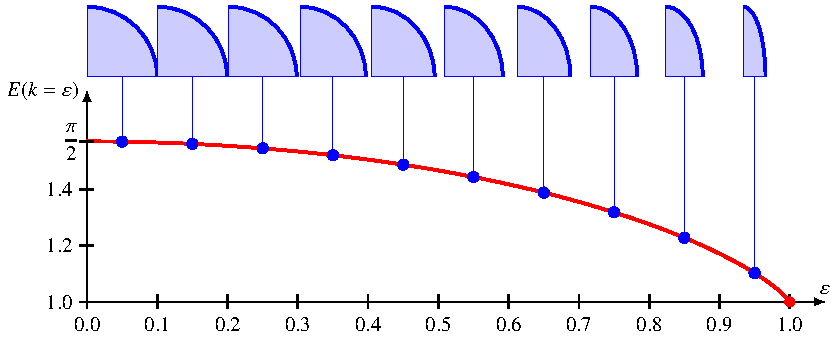
\includegraphics{chapters/110-elliptisch/images/ellipsenumfang.pdf}
\caption{Bogenlänge eines Viertels einer Ellipse mit Exzentrizität
$\varepsilon$.
\label{buch:elliptisch:fig:ellipsenumfang}}
\end{figure}
Wir zeigen, wie sich die Berechnung des Umfangs $U$ einer Ellipse
mit Halbachsen $a$ und $b$, $a\le b$, auf ein volltändiges elliptisches
Integral zurückführen lässt.
Der Fall $a>b$ kann behandelt werden, indem die $x$- und $y$-Koordinaten
vertauscht werden.

Die Parametrisierung
\[
t\mapsto \begin{pmatrix}a\cos t\\ b\sin t\end{pmatrix}
\]
einer Ellipse führt auf das Integral
\begin{align*}
U
&=
\int_0^{2\pi} \sqrt{a^2\sin^2t + b^2\cos^2 t}\,dt
\notag
\\
&=
4\int_0^{\frac{\pi}2}
\sqrt{a^2\sin^2t + b^2(1-\sin^2 t)}
\,dt
\notag
\\
&=
4b \int_0^{\frac{\pi}2} \sqrt{1-(b^2-a^2)/b^2\cdot \sin^2t}\,dt
\label{buch:elliptisch:eqn:umfangellipse}
\end{align*}
für den Umfang der Ellipse.
Bei einem Kreis ist $a=b$ und der zweite Term unter der Wurzel fällt weg,
der Umfang wird $4b\frac{\pi}2=2\pi b$.
Die Differenz $e^2=b^2-a^2$ ist die {\em lineare Exzentrizität} der Ellipse,
\index{lineare Exzentrizität}%
der Quotient $e/b$ wird die {\em numerische Exzentrizität} der Ellipse
genannt.
Insbesondere ist $k = \varepsilon$.

Das Integral~\eqref{buch:elliptisch:eqn:umfangellipse} erhält jetzt die
Form
\[
U
=
4b\int_0^{\frac{\pi}2} \sqrt{1-k^2\sin^2t}\,dt
\]
und ist damit als elliptisches Integral zweiter Art erkannt.
Für den Umfang der Ellipse finden wir damit die Formel
\[
U
=
4b E(k)
=
4b E(\varepsilon).
\]
Das vollständige elliptische Integral zweiter Art $E(\varepsilon)$
liefert also genau den Umfang der eines Viertels Ellipse mit
numerischer Exzentrizität $\varepsilon$ und kleiner Halbachse $1$.

\subsubsection{Komplementäre Integrale}
XXX Komplementäre Integrale \\

\subsubsection{Ableitung}
XXX Ableitung \\
XXX Stammfunktion \\

\subsection{Unvollständige elliptische Integrale}
XXX Vollständige und Unvollständige Integrale \\
XXX Additionstheoreme \\
XXX Parameterkonventionen \\

\subsection{Potenzreihe}
XXX Potenzreihen \\
XXX Als hypergeometrische Funktionen \\



\section{Jacobische elliptische Funktionen}

Für das elliptische Filter werden, wie es der Name bereits deutet, elliptische Funktionen gebraucht.
Wie die trigonometrischen Funktionen Zusammenhänge eines Kreises darlegen, beschreiben die elliptischen Funktionen Ellipsen.
Es ist daher naheliegend, dass der Kosinus des Tschebyscheff-Filters gegen ein elliptisches Pendant ausgetauscht werden könnte.
Der Begriff elliptische Funktion wird für sehr viele Funktionen gebraucht, daher ist es hier wichtig zu erwähnen, dass es ausschliesslich um die Jacobischen elliptischen Funktionen geht.

\subsection{Grundlegende Eigenschaften}

Die Jacobi elliptischen Funktionen werden ausführlich im Kapitel \ref{buch:elliptisch:section:jacobi} behandelt.
Im Wesentlichen erweitern die Jacobi elliptischen Funktionen die trigonometrische Funktionen für Ellipsen.
Zum Beispiel gibt es analog zum Sinus den elliptischen $\sn(z, k)$.
Im Gegensatz zum den trigonometrischen Funktionen haben die elliptischen Funktionen zwei Parameter.
Den \textit{elliptische Modul} $k$, der die Exzentrizität der Ellipse parametrisiert und das Winkelargument $z$.
Im Kreis ist der Radius für alle Winkel konstant, bei Ellipsen ändert sich das.
Dies hat zur Folge, dass bei einer Ellipse die Kreisbogenlänge nicht linear zum Winkel verläuft.
Darum kann hier nicht der gewohnte Winkel verwendet werden.
Das Winkelargument $z$ kann durch das elliptische Integral erster Art
\begin{equation}
    z
    =
    F(\phi, k)
    =
    \int_{0}^{\phi}
    \frac{
        d\theta
    }{
        \sqrt{
            1-k^2 \sin^2 \theta
        }
    }
\end{equation}
mit dem Winkel $\phi$ in Verbindung gebracht werden.

Dabei wird das vollständige und unvollständige elliptische integral unterschieden.
Beim vollständigen Integral
\begin{equation}
    K(k)
    =
    \int_{0}^{\pi / 2}
    \frac{
        d\theta
    }{
        \sqrt{
            1-k^2 \sin^2 \theta
        }
    }
\end{equation}
wird über ein viertel Ellipsenbogen integriert, also bis $\phi=\pi/2$ und liefert das Winkelargument für eine Vierteldrehung.
Die Zahl wird oft auch abgekürzt mit $K = K(k)$ und ist für das elliptische Filter sehr relevant.
Alle elliptischen Funktionen sind somit $4K$-periodisch.

Neben dem $\sn$ gibt es zwei weitere elliptische Basisfunktionen $\cn$ und $\dn$.
Dazu kommen noch weitere abgeleitete Funktionen, die durch Quotienten und Kehrwerte dieser Funktionen zustande kommen.
Insgesamt sind es die zwölf Funktionen
\begin{equation*}
    \sn \quad
    \ns \quad
    \scelliptic \quad
    \sd \quad
    \cn \quad
    \nc \quad
    \cs \quad
    \cd \quad
    \dn \quad
    \nd \quad
    \ds \quad
    \dc.
\end{equation*}

Die Jacobischen elliptischen Funktionen können mit der inversen Funktion des vollständigen elliptischen Integrals erster Art
\begin{equation}
    \phi = F^{-1}(z, k)
\end{equation}
definiert werden. Dabei ist zu beachten dass nur das $z$ Argument der Funktion invertiert wird, also
\begin{equation}
    z = F(\phi, k)
    \Leftrightarrow
    \phi = F^{-1}(z, k).
\end{equation}
Mithilfe von $F^{-1}$ kann zum Beispiel $sn^{-1}$ mit dem elliptischen Integral dargestellt werden:
\begin{equation}
    \sin(\phi)
    =
    \sin \left( F^{-1}(z, k) \right)
    =
    \sn(z, k)
    =
    w.
\end{equation}

% \begin{equation} %TODO remove unnecessary equations
%     \phi
%     =
%      F^{-1}(z, k)
%      =
%      \sin^{-1} \big( \sn (z, k ) \big)
%      =
%     \sin^{-1} ( w )
% \end{equation}

% \begin{equation}
%     F(\phi, k)
%     =
%     z
%     =
%     F( \sin^{-1} \big( \sn (z, k ) \big) , k)
%     =
%     F( \sin^{-1} ( w ), k)
% \end{equation}

% \begin{equation}
%     \sn^{-1}(w, k)
%     =
%     F(\phi, k),
%     \quad
%     \phi = \sin^{-1}(w)
% \end{equation}

\subsection{Die Funktion $\sn^{-1}$}

Beim Tschebyscheff-Filter konnten wir mit Betrachten des Arcuscosinus die Funktionalität erklären.
Für das Elliptische Filter machen wir die gleiche Betrachtung mit der $\sn^{-1}$-Funktion.
Der $\sn^{-1}$ ist durch das elliptische Integral
\begin{align}
    \sn^{-1}(w, k)
        & =
    \int_{0}^{\phi}
    \frac{
        d\theta
    }{
        \sqrt{
            1-k^2 \sin^2 \theta
        }
    },
    \quad
    \phi = \sin^{-1}(w)
    \\
        & =
    \int_{0}^{w}
    \frac{
        dt
    }{
        \sqrt{
            (1-t^2)(1-k^2 t^2)
        }
    }
\end{align}
beschrieben.
Dazu betrachten wir wieder den Integranden
\begin{equation}
    \frac{
        1
    }{
        \sqrt{
            (1-t^2)(1-k^2 t^2)
        }
    }.
\end{equation}
Beim $\cos^{-1}(x)$ haben wir gesehen, dass die analytische Fortsetzung bei $x < -1$ und $x > 1$ rechtwinklig in die komplexen Zahlen wandert.
Wenn man das Gleiche mit $\sn^{-1}(w, k)$ macht, erkennt man zwei interessante Stellen.
Die erste ist die gleiche wie beim $\cos^{-1}(x)$ nämlich bei $t = \pm 1$.
Der erste Term unter der Wurzel wird dann negativ, während der zweite noch positiv ist, da $k \leq 1$.
Ab diesem Punkt knickt die Funktion in die imaginäre Richtung ab.
Bei $t = 1/k$ ist auch der zweite Term negativ und die Funktion verläuft in die negative reelle Richtung.
Abbildung \ref{ellfilter:fig:sn} zeigt den Verlauf der Funktion in der komplexen Ebene.
\begin{figure}
    \centering
    \begin{tikzpicture}[>=stealth', auto, node distance=2cm, scale=1.2]

    \tikzstyle{zero} = [draw, circle, inner sep =0, minimum height=0.15cm]

    \tikzset{pole/.style={cross out, draw=black, minimum size=(0.15cm-\pgflinewidth), inner sep=0pt, outer sep=0pt}}

    \begin{scope}[xscale=0.9, yscale=1.8]

        \draw[gray, ->] (0,-1.5) -- (0,1.5) node[anchor=south]{$\mathrm{Im}~z$};
        \draw[gray, ->] (-5,0) -- (5,0) node[anchor=west]{$\mathrm{Re}~z$};

        \begin{scope}

            \clip(-4.5,-1.25) rectangle (4.5,1.25);

            \fill[yellow!30] (0,0) rectangle (1, 0.5);

            \begin{scope}[xshift=-1cm]

                \foreach \i in {-2,...,2} {
                    \foreach \j in {-2,...,1} {
                        \begin{scope}[xshift=\i*4cm, yshift=\j*1cm]
                            \draw[<-, blue!50] (0, 0) -- (0,0.5);
                            \draw[<-, cyan!50] (1, 0) -- (0,0);
                            \draw[<-, darkgreen!50] (2, 0) -- (1,0);
                            \draw[<-, orange!50] (2,0.5) -- (2, 0);
                            \draw[<-, red!50] (1, 0.5) -- (2,0.5);
                            \draw[<-, purple!50] (0, 0.5) -- (1,0.5);
                            \draw[<-, blue!50] (0,1) -- (0,0.5);
                            \draw[<-, orange!50] (2,0.5) -- (2, 1);
                            \draw[<-, red!50] (3, 0.5) -- (2,0.5);
                            \draw[<-, purple!50] (4, 0.5) -- (3,0.5);
                            \draw[<-, darkgreen!50] (2, 0) -- (3,0);
                            \draw[<-, cyan!50] (3, 0) -- (4,0);
                        \end{scope}
                    }
                }

                % \pause
                \draw[ultra thick, <-, darkgreen] (2, 0) -- (1,0);
                % \pause
                \draw[ultra thick, <-, orange] (2,0.5) -- (2, 0);
                % \pause
                \draw[ultra thick, <-, red] (1, 0.5) -- (2,0.5);
                % \pause
                \draw[ultra thick, <-, blue] (0, 0) -- (0,0.5);
                \draw[ultra thick, <-, purple] (0, 0.5) -- (1,0.5);
                \draw[ultra thick, <-, cyan] (1, 0) -- (0,0);
                % \pause


                \foreach \i in {-2,...,2} {
                    \foreach \j in {-2,...,1} {
                        \begin{scope}[xshift=\i*4cm, yshift=\j*1cm]
                            \node[zero] at ( 1, 0) {};
                            \node[zero] at ( 3, 0) {};
                            \node[pole] at ( 1,0.5) {};
                            \node[pole] at ( 3,0.5) {};
                        \end{scope}
                    }
                }

            \end{scope}

        \end{scope}

        \draw[gray] ( 1,0) +(0,0.1) -- +(0, -0.1) node[inner sep=0, anchor=north] {\small $K$};
        \draw[gray]  (0, 0.5) +(0.1, 0) -- +(-0.1, 0) node[inner sep=0, anchor=east]{\small $jK^\prime$};

    \end{scope}

    \node[zero] at (4,3) (n) {};
    \node[anchor=west] at (n.east) {Zero};
    \node[pole, below=0.25cm of n] (n) {};
    \node[anchor=west] at (n.east) {Pole};

    \begin{scope}[yshift=-4cm, xscale=0.75]

        \draw[gray, ->] (-6,0) -- (6,0) node[anchor=west]{$w$};

        \draw[ultra thick, ->, purple] (-5, 0) -- (-3, 0);
        \draw[ultra thick, ->, blue]      (-3, 0) -- (-2, 0);
        \draw[ultra thick, ->, cyan]       (-2, 0) -- (0, 0);
        \draw[ultra thick, ->, darkgreen]    (0, 0) -- (2, 0);
        \draw[ultra thick, ->, orange] (2, 0) -- (3, 0);
        \draw[ultra thick, ->, red] (3, 0) -- (5, 0);

        \node[anchor=south] at (-5,0) {$-\infty$};
        \node[anchor=south] at (-3,0) {$-1/k$};
        \node[anchor=south] at (-2,0) {$-1$};
        \node[anchor=south] at (0,0) {$0$};
        \node[anchor=south] at (2,0) {$1$};
        \node[anchor=south] at (3,0) {$1/k$};
        \node[anchor=south] at (5,0) {$\infty$};

    \end{scope}


\end{tikzpicture}
    \caption{
        $z$-Ebene der Funktion $z = \sn^{-1}(w, k)$.
        Die Funktion ist in der realen Achse $4K$-periodisch und in der imaginären Achse $2jK^\prime$-periodisch.
    }
    \label{ellfilter:fig:sn}
\end{figure}
In der reellen Richtung ist sie $4K(k)$-periodisch und in der imaginären Richtung $4K^\prime(k)$-periodisch, wobei $K^\prime$ das komplementäre vollständige Elliptische Integral ist:
\begin{equation}
    K^\prime(k)
    =
    \int_{0}^{\pi / 2}
    \frac{
        d\theta
    }{
        \sqrt{
            1-{k^\prime}^2 \sin^2 \theta
        }
    },
    \quad
    k^\prime = \sqrt{1-k^2}.
\end{equation}

%
% lemniskate.tex
%
% (c) 2021 Prof Dr Andreas Müller, OST Ostschweizer Fachhochschule
%
\section{Lemniskatischer Sinus
\label{buch:elliptisch:section:lemniskate}}
\rhead{Lemniskatischer Sinus}
Historisch war der {\em lemniskatische Sinus} die erste ellptische
Funktion, die Gauss bereits als 19-jähriger untersucht, aber nicht 
veröffentlich hat.
In diesem Abschnitt soll die Verbindung zu den Jacobischen
elliptischen Funktionen hergestellt werden.

\subsection{Lemniskate
\label{buch:gemotrie:subsection:lemniskate}}
\begin{figure}
\centering
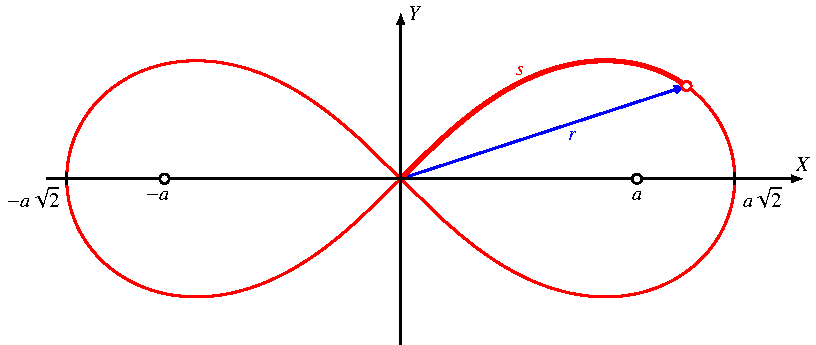
\includegraphics{chapters/110-elliptisch/images/lemniskate.pdf}
\caption{Bogenlänge und Radius der Lemniskate von Bernoulli.
\label{buch:elliptisch:fig:lemniskate}}
\end{figure}
Die Lemniskate von Bernoulli ist die Kurve vierten Grades mit der Gleichung
\begin{equation}
(X^2+Y^2)^2 = 2a^2(X^2-Y^2).
\label{buch:elliptisch:eqn:lemniskate}
\end{equation}
Sie ist in Abbildung~\ref{buch:elliptisch:fig:lemniskate}
dargestellt.
Die beiden Scheitel der Lemniskate befinden sich bei $X_s=\pm a\sqrt{2}$.
Dividiert man die Gleichung der Lemniskate durch $X_s^2=4a^4$ entsteht 
\begin{equation}
\biggl(
\biggl(\frac{X}{a\sqrt{2}}\biggr)^2
+
\biggl(\frac{Y}{a\sqrt{2}}\biggr)^2
\biggr)^2
=
2\frac{a^2}{2a^2}\biggl(
\biggl(\frac{X}{a\sqrt{2}}\biggr)^2
-
\biggl(\frac{Y}{a\sqrt{2}}\biggr)^2
\biggr).
\qquad
\Leftrightarrow
\qquad
(x^2+y^2)^2 = x^2-y^2,
\label{buch:elliptisch:eqn:lemniskatenormiert}
\end{equation}
wobei wir $x=X/a\sqrt{2}$ und $y=Y/a\sqrt{2}$ gesetzt haben.
In dieser Normierung liegen die Scheitel bei $\pm 1$.
Dies ist die Skalierung, die für die Definition des lemniskatischen
Sinus und Kosinus verwendet werden soll.

In Polarkoordinaten $x=r\cos\varphi$ und $y=r\sin\varphi$
gilt nach Einsetzen in \eqref{buch:elliptisch:eqn:lemniskatenormiert}
\begin{equation}
r^4
=
r^2(\cos^2\varphi-\sin^2\varphi)
=
r^2\cos2\varphi
\qquad\Rightarrow\qquad
r^2 = \cos 2\varphi
\label{buch:elliptisch:eqn:lemniskatepolar}
\end{equation}
als Darstellung der Lemniskate in Polardarstellung.
Sie gilt für Winkel $\varphi\in[-\frac{\pi}4,\frac{\pi}4]$ für das
rechte Blatt und $\varphi\in[\frac{3\pi}4,\frac{5\pi}4]$ für das linke
Blatt der Lemniskate.

\subsection{Bogenlänge}
Die Funktionen
\begin{equation}
x(r) = \frac{r}{\sqrt{2}}\sqrt{1+r^2},
\quad
y(r) = \frac{r}{\sqrt{2}}\sqrt{1-r^2}
\label{buch:geometrie:eqn:lemniskateparam}
\end{equation}
erfüllen
\begin{align*}
x(r)^2-y(r)^2
&=
\frac{r^2(1+r^2)}{2}-\frac{r^2(1-r^2)}{2}
\\
&
=
r^4
=
(x(r)^2 + y(r)^2)^2,
\end{align*}
sie stellen also eine Parametrisierung der Lemniskate dar.

Mit Hilfe der Parametrisierung~\eqref{buch:geometrie:eqn:lemniskateparam}
kann man die Länge $s$ des in Abbildung~\ref{buch:elliptisch:fig:lemniskate}
dargestellten Bogens der Lemniskate berechnen.
Dazu benötigt man die Ableitungen nach $r$, die man mit der Produkt- und
Kettenregel berechnen kann:
\begin{align*}
\dot{x}(r)
&=
\frac{\sqrt{1+r^2}}{\sqrt{2}}
+
\frac{r^2}{\sqrt{2}\sqrt{1+r^2}}
&&\Rightarrow&
\dot{x}(r)^2
&=
\frac{1+r^2}{2} +r^2 + \frac{r^4}{2(1+r^2)}
\\
\dot{y}(r)
&=
\frac{\sqrt{1-r^2}}{\sqrt{2}}
-
\frac{r^2}{\sqrt{2}\sqrt{1-r^2}}
&&\Rightarrow&
\dot{y}(r)^2
&=
\frac{1-r^2}{2} -r^2 + \frac{r^4}{2(1-r^2)}
\end{align*}
Die Summe der Quadrate ist
\begin{align*}
\dot{x}(r)^2 + \dot{y}(r)^2
&=
1 + r^4\frac{1-r^2+1+r^2}{2(1+r^2)(1-r^2)}
=
1+r^4\frac{2}{2(1-r^4)}
=
\frac{1-r^4+r^4}{1-r^4}
=
\frac1{1-r^4}.
\end{align*}
Durch Einsetzen in das Integral für die Bogenlänge bekommt man
\begin{equation}
s(r)
=
\int_0^r
\frac{1}{\sqrt{1-t^4}}\,dt.
\label{buch:elliptisch:eqn:lemniskatebogenlaenge}
\end{equation}

%
% Als elliptisches Integral
%
\subsection{Darstellung als elliptisches Integral}
Das unvollständige elliptische Integral erster Art mit Parameter
$k^2=-1$ oder $k=i$ ist
\[
K(r,i)
=
\int_0^x \frac{dt}{\sqrt{(1-t^2)(1-i^2 t^2)}}
=
\int_0^x \frac{dt}{\sqrt{(1-t^2)(1-(-1)t^2)}}
=
\int_0^x \frac{dt}{\sqrt{1-t^4}}
=
s(r).
\]
Der lemniskatische Sinus ist also eine Umkehrfunktion des
elliptischen Integrals erster Art für den speziellen Wert $i$ des
Parameters $k$.

Die Länge des rechten Blattes der Lemniskate wird mit $\varpi$ bezeichnet
und hat den numerischen Wert
\[
\varpi
=
2\int_0^1\sqrt{\frac{1}{1-t^4}}\,dt
=
2.6220575542.
\]
$\varpi$ ist auch als die {\em lemniskatische Konstante} bekannt.
\index{lemniskatische Konstante}%
Der Lemniskatenbogen zwischen dem Nullpunkt und $(1,0)$ hat die Länge
$\varpi/2$.

%
%  Bogenlängenparametrisierung
%
\subsection{Bogenlängenparametrisierung}
Die Lemniskate mit der Gleichung
\[
(X^2+X^2)^2=2(X^2-X^2)
\]
(der Fall $a=1$ in \eqref{buch:elliptisch:eqn:lemniskate})
kann mit Jacobischen elliptischen Funktionen
parametrisiert werden.
Dazu schreibt man
\[
\left.
\begin{aligned}
X(t)
&=
\sqrt{2}\operatorname{cn}(t,k) \operatorname{dn}(t,k)
\\
Y(t)
&=
\phantom{\sqrt{2}}
\operatorname{cn}(t,k) \operatorname{sn}(t,k)
\end{aligned}
\quad\right\}
\qquad\text{mit $k=\displaystyle\frac{1}{\sqrt{2}}$}
\]
und berechnet die beiden Seiten der definierenden Gleichung der
Lemniskate.
Zunächst ist
\begin{align*}
X(t)^2
&=
2\operatorname{cn}(t,k)^2
\operatorname{dn}(t,k)^2
\\
Y(t)^2
&=
\operatorname{cn}(t,k)^2
\operatorname{sn}(t,k)^2
\\
X(t)^2+Y(t)^2
&=
2\operatorname{cn}(t,k)^2
\bigl(
\underbrace{
\operatorname{dn}(t,k)^2
+{\textstyle\frac12}
\operatorname{sn}(t,k)^2
}_{\displaystyle =1}
\bigr)
%\\
%&
=
2\operatorname{cn}(t,k)^2
\\
X(t)^2-Y(t)^2
&=
\operatorname{cn}(t,k)^2
\bigl(
2\operatorname{dn}(t,k)^2 - \operatorname{sn}(t,k)^2
\bigr)
\\
&=
\operatorname{cn}(t,k)^2
\bigl(
2\bigl({\textstyle\frac12}+{\textstyle\frac12}\operatorname{cn}(t,k)^2\bigr)
-
\bigl(1-\operatorname{cn}(t,k)^2\bigr)
\bigr)
\\
&=
2\operatorname{cn}(t,k)^4
\\
\Rightarrow\qquad
(X(t)^2+Y(t)^2)^2
&=
4\operatorname{cn}(t,k)^4
=
2(X(t)^2-Y(t)^2).
\end{align*}
Wir zeigen jetzt, dass dies tatsächlich eine Bogenlängenparametrisierung
der Lemniskate ist.
Dazu berechnen wir die Ableitungen
\begin{align*}
\dot{X}(t)
&=
\sqrt{2}\operatorname{cn}'(t,k)\operatorname{dn}(t,k)
+
\sqrt{2}\operatorname{cn}(t,k)\operatorname{dn}'(t,k)
\\
&=
-\sqrt{2}\operatorname{sn}(t,k)\operatorname{dn}(t,k)^2
-\frac12\sqrt{2}\operatorname{sn}(t,k)\operatorname{cn}(t,k)^2
\\
&=
-\sqrt{2}\operatorname{sn}(t,k)\bigl(
1-{\textstyle\frac12}\operatorname{sn}(t,k)^2
+{\textstyle\frac12}-{\textstyle\frac12}\operatorname{sn}(u,t)^2
\bigr)
\\
&=
\sqrt{2}\operatorname{sn}(t,k)
\bigl(
{\textstyle \frac32}-\operatorname{sn}(t,k)^2
\bigr)
\\
\dot{X}(t)^2
&=
2\operatorname{sn}(t,k)^2
\bigl(
{\textstyle \frac32}-\operatorname{sn}(t,k)^2
\bigr)^2
\\
&=
{\textstyle\frac{9}{2}}\operatorname{sn}(t,k)^2
-
6\operatorname{sn}(t,k)^4
+2\operatorname{sn}(t,k)^6
\\
\dot{Y}(t)
&=
\operatorname{cn}'(t,k)\operatorname{sn}(t,k)
+
\operatorname{cn}(t,k)\operatorname{sn}'(t,k)
\\
&=
-\operatorname{sn}(t,k)^2
\operatorname{dn}(t,k)
+\operatorname{cn}(t,k)^2
\operatorname{dn}(t,k)
\\
&=
\operatorname{dn}(t,k)\bigl(1-2\operatorname{sn}(t,k)^2\bigr)
\\
\dot{Y}(t)^2
&=
\bigl(1-{\textstyle\frac12}\operatorname{sn}(t,k)^2\bigr)
\bigl(1-2\operatorname|{sn}(t,k)^2\bigr)^2
\\
&=
1-{\textstyle\frac{9}{2}}\operatorname{sn}(t,k)^2
+6\operatorname{sn}(t,k)^4
-2\operatorname{sn}(t,k)^6
\\
\dot{X}(t)^2 + \dot{Y}(t)^2
&=
1.
\end{align*}
Dies bedeutet, dass die Bogenlänge zwischen den Parameterwerten $0$ und $s$
\[
\int_0^s
\sqrt{\dot{X}(t)^2 + \dot{Y}(t)^2}
\,dt
=
\int_0^s\,dt
=
s,
\]
der Parameter $t$ ist also ein Bogenlängenparameter.

Die mit dem Faktor $1/\sqrt{2}$ skalierte Standard-Lemniskate mit der
Gleichung
\[
(x^2+y^2)^2 = x^2-y^2
\]
hat daher eine Bogenlängenparametrisierung mit
\begin{equation}
\begin{aligned}
x(t)
&=
\phantom{\frac{1}{\sqrt{2}}}
\operatorname{cn}(\sqrt{2}t,k)\operatorname{dn}(\sqrt{2}t,k)
\\
y(t)
&=
\frac{1}{\sqrt{2}}\operatorname{cn}(\sqrt{2}t,k)\operatorname{sn}(\sqrt{2}t,k)
\end{aligned}
\label{buch:elliptisch:lemniskate:bogenlaenge}
\end{equation}

\subsection{Der lemniskatische Sinus und Kosinus}
Der Sinus Berechnet die Gegenkathete zu einer gegebenen Bogenlänge des
Kreises, er ist die Umkehrfunktion der Funktion, die der Gegenkathete
die Bogenlänge zuordnet.

Daher ist es naheliegend, die Umkehrfunktion von $s(r)$ in 
\eqref{buch:elliptisch:eqn:lemniskatebogenlaenge}
den {\em lemniskatischen Sinus} zu nennen mit der Bezeichnung
$r=\operatorname{sl} s$.

Der Kosinus ist der Sinus des komplementären Winkels.
Auch für die lemniskatische Bogenlänge $s(r)$ lässt sich eine
komplementäre Bogenlänge definieren, nämlich die Bogenlänge zwischen
dem Punkt $(x(r), y(r))$ und $(1,0)$.

Da die Parametrisierung~\eqref{buch:elliptisch:lemniskate:bogenlaenge}
eine Bogenlängenparametrisierung ist, darf man $t=s$ schreiben.
Dann kann man aber auch $r(s)$ daraus berechnen,
es ist
\[
r(s)^2
=
x(s)^2 + y(s)^2
=
\operatorname{cn}(s\sqrt{2},k)^2
\qquad\Rightarrow\qquad
r(s)
=
\operatorname{cn}(s\sqrt{2},k)
\]

\begin{figure}
\centering
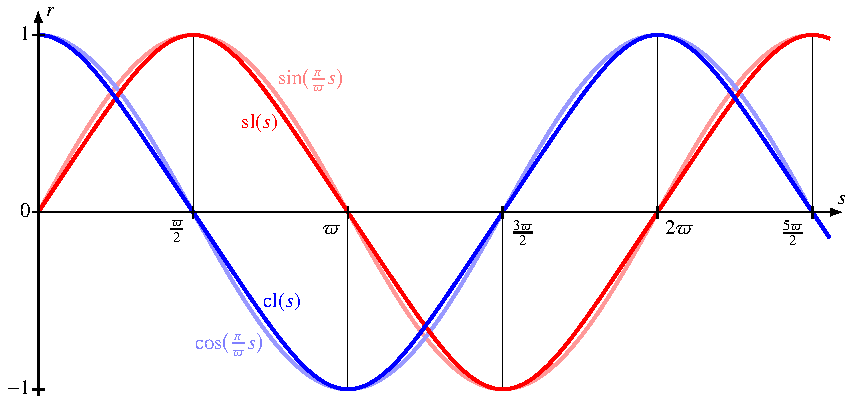
\includegraphics{chapters/110-elliptisch/images/slcl.pdf}
\caption{
Lemniskatischer Sinus und Kosinus sowie Sinus und Kosinus
mit derart skaliertem Argument, dass die Funktionen die gleichen Nullstellen
haben.
\label{buch:elliptisch:figure:slcl}}
\end{figure}


%\section*{Übungsaufgaben}
%\rhead{Übungsaufgaben}
%\aufgabetoplevel{chapters/020-exponential/uebungsaufgaben}
%\begin{uebungsaufgaben}
%\uebungsaufgabe{0}
%\uebungsaufgabe{1}
%\end{uebungsaufgaben}


%%
% chapter.tex -- Beschreibung des Inhaltes
%
% (c) 2021 Prof Dr Andreas Müller, Hochschule Rapperswil
%
% !TeX spellcheck = de_CH
\chapter{Elliptische Funktionen
\label{buch:chapter:geometrie}}
\lhead{Elliptische Funktionen}
\rhead{}

Der Versuch, die Länge eines Ellipsenbogens zu berechnen, hat
in Abschnitt~\ref{buch:geometrie:subsection:hyperbeln-und-ellipsen}
zu Integralen geführt, die nicht in geschlossener Form ausgewertet
werden können.
Neben den dort gefundenen Integralen sind noch weitere, ähnlich
aufgebaute Integrale in dieser Familie zu finden.

%
% ellintegral.tex
%
% (c) 2021 Prof Dr Andreas Müller, OST Ostschweizer Fachhochschule
%
\section{Elliptische Integrale
\label{buch:elliptisch:section:integral}}
\rhead{Elliptisches Integral}
Bei der Berechnung des Ellipsenbogens in 
Abschnitt~\ref{buch:geometrie:subsection:hyperbeln-und-ellipsen}
sind wir auf ein Integral gestossen, welches sich nicht in geschlossener
Form ausdrücken liess.
Um solche Integrale in den Griff zu bekommen, ist es nötig, sie als
neue spezielle Funktionen zu definieren.

\subsection{Definition
\label{buch:elliptisch:subsection:definition}}
Ein {\em elliptisches Integral} ist ein Integral der Form
\index{elliptishes Integral}%
\index{Integral, elliptisch}%
\begin{equation}
\int R\left( x, \sqrt{p(x)}\right)\,dx
\label{buch:elliptisch:def:allgemein}
\end{equation}
wobei $R(x,y)$ eine rationale Funktion von zwei Variablen ist und
$p(x)$ ein Polynom dritten oder vierten Grades.
Hätte $p(x)$ ein mehrfache Nullstelle $x_0$, müsste es durch $(x-x_0)^2$
teilbar sein, man könnte also einen Faktor $(x-x_0)$ aus der
Wurzel im Integraneden von \eqref{buch:elliptisch:def:allgemein}
ausklammern und damit das Integral in eine Form bringen, wo $p(x)$
höchstens zweiten Grades ist.
Solche Integrale lassen sich meistens mit trigonometrischen Substitutionen
berechnen.
Wir verlangen daher, dass $p(x)$ keine mehrfachen Nullstellen hat.

Man kann zeigen, dass sich elliptische Integrale in Summen von
elementaren Funktionen und speziellen elliptischen Integralen 
der folgenden Form überführen lassen
\cite[Abschnitt 164, p.~506]{buch:smirnov32}.

\begin{definition}
\label{buch:elliptisch:def:integrale123}
Die elliptischen Integrale erster, zweiter und dritter Art sind die
Integrale
\[
\begin{aligned}
\text{1.~Art:}&&&
\int \frac{dx}{\sqrt{(1-x^2)(1-k^2x^2)}}
\\
\text{2.~Art:}&&&
\int \sqrt{\frac{1-k^2x^2}{1-x^2}}\,dx
\\
\text{3.~Art:}&&&
\int \frac{dx}{(1-nx^2)\sqrt{(1-x^2)(1-k^2x^2)}}
\end{aligned}
\]
mit $0<k<1$.
Es ist auch üblich, den Parameter $m=k^2$ zu verwenden.
\end{definition}

Wie gesagt lassen sich für diese unbestimmten Integrale keine 
geschlossenen Formen finden.
Es bleibt uns daher nichts anderes übrig, als die Integralgrenzen
festzulegen und damit eine Stammfunktion auszuwählen.

%
% Elliptisches Integral
%
\subsection{Vollständige elliptische Integrale
\label{buch:elliptisch:subsection:vollstaendig}}
In diesem Abschnitt legen wir beide Integrationsgrenzen fest und
untersuchen die entstehenenden Funktionen von den Parametern
$k$ und $n$.

\subsubsection{Definition der vollständigen elliptischen Integrale}
Da der Nenner in allen drei elliptischen Integralen eine Nullstelle
bei $\pm1$ hat, kann das Integral nur von $0$ bis $1$ erstreckt werden.

\begin{definition}
\label{buch:elliptisch:def:vollstintegrale123}
Die vollständigen elliptischen Integrale erster, zweiter und dritter
Art sind
\[
\begin{aligned}
\text{1.~Art:}&&
K(k)&=\int_0^1 \frac{dt}{\sqrt{(1-t^2)(1-k^2t^2)}} \\
\text{2.~Art:}&&
E(k)&=\int_0^1 \sqrt{\frac{1-k^2t^2}{1-t^2}}\,dt \\
\text{3.~Art:}&&
\Pi(n, k)&=\int_0^1\frac{dt}{(1-nt^2)\sqrt{(1-t^2)(1-k^2t^2)}} 
\end{aligned}
\]
mit $0<k<1$.
\end{definition}

Die Funktionen hängen stetig von $k$ ab.
Die Nullstellen des Faktors $1-k^2x^2$ liegen ausserhalb des
Integrationsintervalls und spielen daher keine Rolle.
Die Werte von $K(k)$ und $E(k)$ für $k=0$ können direkt berechnet
werden:
\begin{align*}
K(0)
=
E(0)
&=
\int_0^1 \frac{dt}{\sqrt{1-t^2}}=\frac{\pi}2.
\end{align*}
Das Integral $\Pi(n,0)$ ist etwas komplizierter.

Für $k\to 1$ ist $E(k)=1$, die Integrale $K(1)$ und $\Pi(n,1)$
sind dagegen divergent.

\subsubsection{Jacobi- und Legendre-Normalform}
Die Integrationsvariable $t$ der vollständigen elliptischen Integrale
kann durch die Substitution $t=\sin\varphi$ durch die Variable
$\varphi$ und das Integral über das Intervall $[0,1]$ durch ein
Integral über das Intervall $[0,\frac{\pi}2]$ ersetzt werden.
Mit
\[
\frac{dt}{d\varphi} = \cos\varphi = \sqrt{1-\sin^2\varphi}
\]
können die Funktionen $K(k)$, $E(k)$ und $\Pi(n,k)$ auch als
\begin{align*}
K(k)
&=
\int_0^{\frac{\pi}2}
\frac{
\sqrt{1-\sin^2\varphi}\,d\varphi
}{
\sqrt{(1-\sin^2\varphi)(1-k^2\sin^2\varphi)}
}
=
\int_0^{\frac{\pi}2}
\frac{d\varphi}{\sqrt{1-k^2\sin^2\varphi}}
\\
E(k)
&=
\int_0^{\frac{\pi}2}
\sqrt{\frac{1-k^2\sin^2\varphi}{1-\sin^2\varphi}}\sqrt{1-\sin^2\varphi}\,d\varphi
=
\int_0^{\frac{\pi}2}
\sqrt{1-k^2\sin^2\varphi}\,d\varphi
\\
\Pi(n,k)
&=
\int_0^{\frac{\pi}2}
\frac{
\sqrt{1-\sin^2\varphi}\,d\varphi
}{
(1-n\sin^2\varphi)\sqrt{(1-\sin^2\varphi)(1-k^2\sin^2\varphi)}
}
=
\int_0^{\frac{\pi}2}
\frac{
d\varphi
}{
(1-n\sin^2\varphi)\sqrt{1-k^2\sin^2\varphi}
}
\end{align*}
Diese Form wird auch die {\em Legendre-Normalform} der vollständigen 
\index{Legendre-Normalform}%
elliptischen Integrale genannt, während die Form von
Definition~\ref{buch:elliptisch:def:vollstintegrale123}
die {\em Jacobi-Normalform} heisst.
\index{Jacobi-Normalform}%

\subsubsection{Umfang einer Ellipse}
\begin{figure}
\centering
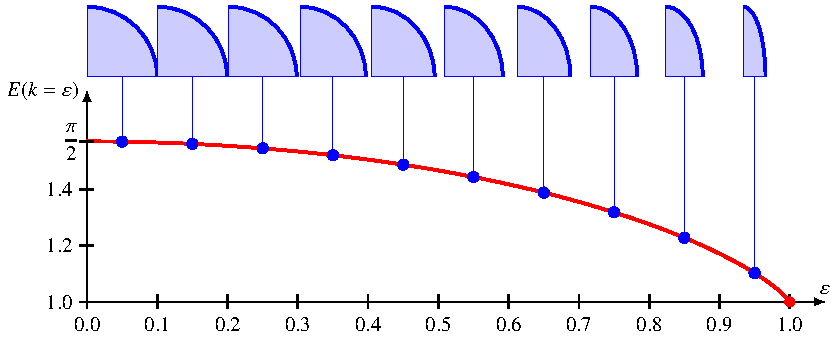
\includegraphics{chapters/110-elliptisch/images/ellipsenumfang.pdf}
\caption{Bogenlänge eines Viertels einer Ellipse mit Exzentrizität
$\varepsilon$.
\label{buch:elliptisch:fig:ellipsenumfang}}
\end{figure}
Wir zeigen, wie sich die Berechnung des Umfangs $U$ einer Ellipse
mit Halbachsen $a$ und $b$, $a\le b$, auf ein volltändiges elliptisches
Integral zurückführen lässt.
Der Fall $a>b$ kann behandelt werden, indem die $x$- und $y$-Koordinaten
vertauscht werden.

Die Parametrisierung
\[
t\mapsto \begin{pmatrix}a\cos t\\ b\sin t\end{pmatrix}
\]
einer Ellipse führt auf das Integral
\begin{align*}
U
&=
\int_0^{2\pi} \sqrt{a^2\sin^2t + b^2\cos^2 t}\,dt
\notag
\\
&=
4\int_0^{\frac{\pi}2}
\sqrt{a^2\sin^2t + b^2(1-\sin^2 t)}
\,dt
\notag
\\
&=
4b \int_0^{\frac{\pi}2} \sqrt{1-(b^2-a^2)/b^2\cdot \sin^2t}\,dt
\label{buch:elliptisch:eqn:umfangellipse}
\end{align*}
für den Umfang der Ellipse.
Bei einem Kreis ist $a=b$ und der zweite Term unter der Wurzel fällt weg,
der Umfang wird $4b\frac{\pi}2=2\pi b$.
Die Differenz $e^2=b^2-a^2$ ist die {\em lineare Exzentrizität} der Ellipse,
\index{lineare Exzentrizität}%
der Quotient $e/b$ wird die {\em numerische Exzentrizität} der Ellipse
genannt.
Insbesondere ist $k = \varepsilon$.

Das Integral~\eqref{buch:elliptisch:eqn:umfangellipse} erhält jetzt die
Form
\[
U
=
4b\int_0^{\frac{\pi}2} \sqrt{1-k^2\sin^2t}\,dt
\]
und ist damit als elliptisches Integral zweiter Art erkannt.
Für den Umfang der Ellipse finden wir damit die Formel
\[
U
=
4b E(k)
=
4b E(\varepsilon).
\]
Das vollständige elliptische Integral zweiter Art $E(\varepsilon)$
liefert also genau den Umfang der eines Viertels Ellipse mit
numerischer Exzentrizität $\varepsilon$ und kleiner Halbachse $1$.

\subsubsection{Komplementäre Integrale}
XXX Komplementäre Integrale \\

\subsubsection{Ableitung}
XXX Ableitung \\
XXX Stammfunktion \\

\subsection{Unvollständige elliptische Integrale}
XXX Vollständige und Unvollständige Integrale \\
XXX Additionstheoreme \\
XXX Parameterkonventionen \\

\subsection{Potenzreihe}
XXX Potenzreihen \\
XXX Als hypergeometrische Funktionen \\



\section{Jacobische elliptische Funktionen}

Für das elliptische Filter werden, wie es der Name bereits deutet, elliptische Funktionen gebraucht.
Wie die trigonometrischen Funktionen Zusammenhänge eines Kreises darlegen, beschreiben die elliptischen Funktionen Ellipsen.
Es ist daher naheliegend, dass der Kosinus des Tschebyscheff-Filters gegen ein elliptisches Pendant ausgetauscht werden könnte.
Der Begriff elliptische Funktion wird für sehr viele Funktionen gebraucht, daher ist es hier wichtig zu erwähnen, dass es ausschliesslich um die Jacobischen elliptischen Funktionen geht.

\subsection{Grundlegende Eigenschaften}

Die Jacobi elliptischen Funktionen werden ausführlich im Kapitel \ref{buch:elliptisch:section:jacobi} behandelt.
Im Wesentlichen erweitern die Jacobi elliptischen Funktionen die trigonometrische Funktionen für Ellipsen.
Zum Beispiel gibt es analog zum Sinus den elliptischen $\sn(z, k)$.
Im Gegensatz zum den trigonometrischen Funktionen haben die elliptischen Funktionen zwei Parameter.
Den \textit{elliptische Modul} $k$, der die Exzentrizität der Ellipse parametrisiert und das Winkelargument $z$.
Im Kreis ist der Radius für alle Winkel konstant, bei Ellipsen ändert sich das.
Dies hat zur Folge, dass bei einer Ellipse die Kreisbogenlänge nicht linear zum Winkel verläuft.
Darum kann hier nicht der gewohnte Winkel verwendet werden.
Das Winkelargument $z$ kann durch das elliptische Integral erster Art
\begin{equation}
    z
    =
    F(\phi, k)
    =
    \int_{0}^{\phi}
    \frac{
        d\theta
    }{
        \sqrt{
            1-k^2 \sin^2 \theta
        }
    }
\end{equation}
mit dem Winkel $\phi$ in Verbindung gebracht werden.

Dabei wird das vollständige und unvollständige elliptische integral unterschieden.
Beim vollständigen Integral
\begin{equation}
    K(k)
    =
    \int_{0}^{\pi / 2}
    \frac{
        d\theta
    }{
        \sqrt{
            1-k^2 \sin^2 \theta
        }
    }
\end{equation}
wird über ein viertel Ellipsenbogen integriert, also bis $\phi=\pi/2$ und liefert das Winkelargument für eine Vierteldrehung.
Die Zahl wird oft auch abgekürzt mit $K = K(k)$ und ist für das elliptische Filter sehr relevant.
Alle elliptischen Funktionen sind somit $4K$-periodisch.

Neben dem $\sn$ gibt es zwei weitere elliptische Basisfunktionen $\cn$ und $\dn$.
Dazu kommen noch weitere abgeleitete Funktionen, die durch Quotienten und Kehrwerte dieser Funktionen zustande kommen.
Insgesamt sind es die zwölf Funktionen
\begin{equation*}
    \sn \quad
    \ns \quad
    \scelliptic \quad
    \sd \quad
    \cn \quad
    \nc \quad
    \cs \quad
    \cd \quad
    \dn \quad
    \nd \quad
    \ds \quad
    \dc.
\end{equation*}

Die Jacobischen elliptischen Funktionen können mit der inversen Funktion des vollständigen elliptischen Integrals erster Art
\begin{equation}
    \phi = F^{-1}(z, k)
\end{equation}
definiert werden. Dabei ist zu beachten dass nur das $z$ Argument der Funktion invertiert wird, also
\begin{equation}
    z = F(\phi, k)
    \Leftrightarrow
    \phi = F^{-1}(z, k).
\end{equation}
Mithilfe von $F^{-1}$ kann zum Beispiel $sn^{-1}$ mit dem elliptischen Integral dargestellt werden:
\begin{equation}
    \sin(\phi)
    =
    \sin \left( F^{-1}(z, k) \right)
    =
    \sn(z, k)
    =
    w.
\end{equation}

% \begin{equation} %TODO remove unnecessary equations
%     \phi
%     =
%      F^{-1}(z, k)
%      =
%      \sin^{-1} \big( \sn (z, k ) \big)
%      =
%     \sin^{-1} ( w )
% \end{equation}

% \begin{equation}
%     F(\phi, k)
%     =
%     z
%     =
%     F( \sin^{-1} \big( \sn (z, k ) \big) , k)
%     =
%     F( \sin^{-1} ( w ), k)
% \end{equation}

% \begin{equation}
%     \sn^{-1}(w, k)
%     =
%     F(\phi, k),
%     \quad
%     \phi = \sin^{-1}(w)
% \end{equation}

\subsection{Die Funktion $\sn^{-1}$}

Beim Tschebyscheff-Filter konnten wir mit Betrachten des Arcuscosinus die Funktionalität erklären.
Für das Elliptische Filter machen wir die gleiche Betrachtung mit der $\sn^{-1}$-Funktion.
Der $\sn^{-1}$ ist durch das elliptische Integral
\begin{align}
    \sn^{-1}(w, k)
        & =
    \int_{0}^{\phi}
    \frac{
        d\theta
    }{
        \sqrt{
            1-k^2 \sin^2 \theta
        }
    },
    \quad
    \phi = \sin^{-1}(w)
    \\
        & =
    \int_{0}^{w}
    \frac{
        dt
    }{
        \sqrt{
            (1-t^2)(1-k^2 t^2)
        }
    }
\end{align}
beschrieben.
Dazu betrachten wir wieder den Integranden
\begin{equation}
    \frac{
        1
    }{
        \sqrt{
            (1-t^2)(1-k^2 t^2)
        }
    }.
\end{equation}
Beim $\cos^{-1}(x)$ haben wir gesehen, dass die analytische Fortsetzung bei $x < -1$ und $x > 1$ rechtwinklig in die komplexen Zahlen wandert.
Wenn man das Gleiche mit $\sn^{-1}(w, k)$ macht, erkennt man zwei interessante Stellen.
Die erste ist die gleiche wie beim $\cos^{-1}(x)$ nämlich bei $t = \pm 1$.
Der erste Term unter der Wurzel wird dann negativ, während der zweite noch positiv ist, da $k \leq 1$.
Ab diesem Punkt knickt die Funktion in die imaginäre Richtung ab.
Bei $t = 1/k$ ist auch der zweite Term negativ und die Funktion verläuft in die negative reelle Richtung.
Abbildung \ref{ellfilter:fig:sn} zeigt den Verlauf der Funktion in der komplexen Ebene.
\begin{figure}
    \centering
    \begin{tikzpicture}[>=stealth', auto, node distance=2cm, scale=1.2]

    \tikzstyle{zero} = [draw, circle, inner sep =0, minimum height=0.15cm]

    \tikzset{pole/.style={cross out, draw=black, minimum size=(0.15cm-\pgflinewidth), inner sep=0pt, outer sep=0pt}}

    \begin{scope}[xscale=0.9, yscale=1.8]

        \draw[gray, ->] (0,-1.5) -- (0,1.5) node[anchor=south]{$\mathrm{Im}~z$};
        \draw[gray, ->] (-5,0) -- (5,0) node[anchor=west]{$\mathrm{Re}~z$};

        \begin{scope}

            \clip(-4.5,-1.25) rectangle (4.5,1.25);

            \fill[yellow!30] (0,0) rectangle (1, 0.5);

            \begin{scope}[xshift=-1cm]

                \foreach \i in {-2,...,2} {
                    \foreach \j in {-2,...,1} {
                        \begin{scope}[xshift=\i*4cm, yshift=\j*1cm]
                            \draw[<-, blue!50] (0, 0) -- (0,0.5);
                            \draw[<-, cyan!50] (1, 0) -- (0,0);
                            \draw[<-, darkgreen!50] (2, 0) -- (1,0);
                            \draw[<-, orange!50] (2,0.5) -- (2, 0);
                            \draw[<-, red!50] (1, 0.5) -- (2,0.5);
                            \draw[<-, purple!50] (0, 0.5) -- (1,0.5);
                            \draw[<-, blue!50] (0,1) -- (0,0.5);
                            \draw[<-, orange!50] (2,0.5) -- (2, 1);
                            \draw[<-, red!50] (3, 0.5) -- (2,0.5);
                            \draw[<-, purple!50] (4, 0.5) -- (3,0.5);
                            \draw[<-, darkgreen!50] (2, 0) -- (3,0);
                            \draw[<-, cyan!50] (3, 0) -- (4,0);
                        \end{scope}
                    }
                }

                % \pause
                \draw[ultra thick, <-, darkgreen] (2, 0) -- (1,0);
                % \pause
                \draw[ultra thick, <-, orange] (2,0.5) -- (2, 0);
                % \pause
                \draw[ultra thick, <-, red] (1, 0.5) -- (2,0.5);
                % \pause
                \draw[ultra thick, <-, blue] (0, 0) -- (0,0.5);
                \draw[ultra thick, <-, purple] (0, 0.5) -- (1,0.5);
                \draw[ultra thick, <-, cyan] (1, 0) -- (0,0);
                % \pause


                \foreach \i in {-2,...,2} {
                    \foreach \j in {-2,...,1} {
                        \begin{scope}[xshift=\i*4cm, yshift=\j*1cm]
                            \node[zero] at ( 1, 0) {};
                            \node[zero] at ( 3, 0) {};
                            \node[pole] at ( 1,0.5) {};
                            \node[pole] at ( 3,0.5) {};
                        \end{scope}
                    }
                }

            \end{scope}

        \end{scope}

        \draw[gray] ( 1,0) +(0,0.1) -- +(0, -0.1) node[inner sep=0, anchor=north] {\small $K$};
        \draw[gray]  (0, 0.5) +(0.1, 0) -- +(-0.1, 0) node[inner sep=0, anchor=east]{\small $jK^\prime$};

    \end{scope}

    \node[zero] at (4,3) (n) {};
    \node[anchor=west] at (n.east) {Zero};
    \node[pole, below=0.25cm of n] (n) {};
    \node[anchor=west] at (n.east) {Pole};

    \begin{scope}[yshift=-4cm, xscale=0.75]

        \draw[gray, ->] (-6,0) -- (6,0) node[anchor=west]{$w$};

        \draw[ultra thick, ->, purple] (-5, 0) -- (-3, 0);
        \draw[ultra thick, ->, blue]      (-3, 0) -- (-2, 0);
        \draw[ultra thick, ->, cyan]       (-2, 0) -- (0, 0);
        \draw[ultra thick, ->, darkgreen]    (0, 0) -- (2, 0);
        \draw[ultra thick, ->, orange] (2, 0) -- (3, 0);
        \draw[ultra thick, ->, red] (3, 0) -- (5, 0);

        \node[anchor=south] at (-5,0) {$-\infty$};
        \node[anchor=south] at (-3,0) {$-1/k$};
        \node[anchor=south] at (-2,0) {$-1$};
        \node[anchor=south] at (0,0) {$0$};
        \node[anchor=south] at (2,0) {$1$};
        \node[anchor=south] at (3,0) {$1/k$};
        \node[anchor=south] at (5,0) {$\infty$};

    \end{scope}


\end{tikzpicture}
    \caption{
        $z$-Ebene der Funktion $z = \sn^{-1}(w, k)$.
        Die Funktion ist in der realen Achse $4K$-periodisch und in der imaginären Achse $2jK^\prime$-periodisch.
    }
    \label{ellfilter:fig:sn}
\end{figure}
In der reellen Richtung ist sie $4K(k)$-periodisch und in der imaginären Richtung $4K^\prime(k)$-periodisch, wobei $K^\prime$ das komplementäre vollständige Elliptische Integral ist:
\begin{equation}
    K^\prime(k)
    =
    \int_{0}^{\pi / 2}
    \frac{
        d\theta
    }{
        \sqrt{
            1-{k^\prime}^2 \sin^2 \theta
        }
    },
    \quad
    k^\prime = \sqrt{1-k^2}.
\end{equation}

%
% lemniskate.tex
%
% (c) 2021 Prof Dr Andreas Müller, OST Ostschweizer Fachhochschule
%
\section{Lemniskatischer Sinus
\label{buch:elliptisch:section:lemniskate}}
\rhead{Lemniskatischer Sinus}
Historisch war der {\em lemniskatische Sinus} die erste ellptische
Funktion, die Gauss bereits als 19-jähriger untersucht, aber nicht 
veröffentlich hat.
In diesem Abschnitt soll die Verbindung zu den Jacobischen
elliptischen Funktionen hergestellt werden.

\subsection{Lemniskate
\label{buch:gemotrie:subsection:lemniskate}}
\begin{figure}
\centering
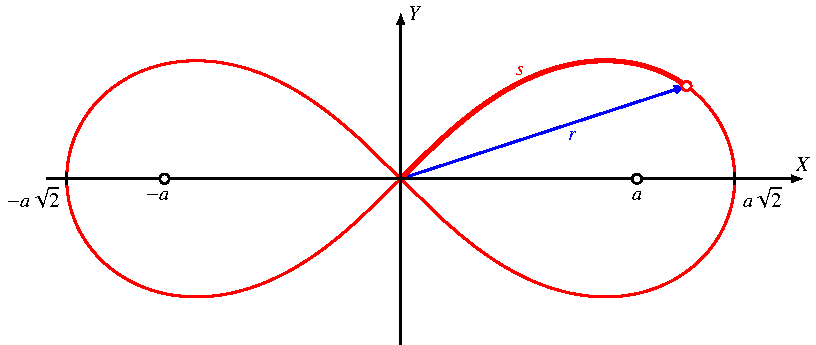
\includegraphics{chapters/110-elliptisch/images/lemniskate.pdf}
\caption{Bogenlänge und Radius der Lemniskate von Bernoulli.
\label{buch:elliptisch:fig:lemniskate}}
\end{figure}
Die Lemniskate von Bernoulli ist die Kurve vierten Grades mit der Gleichung
\begin{equation}
(X^2+Y^2)^2 = 2a^2(X^2-Y^2).
\label{buch:elliptisch:eqn:lemniskate}
\end{equation}
Sie ist in Abbildung~\ref{buch:elliptisch:fig:lemniskate}
dargestellt.
Die beiden Scheitel der Lemniskate befinden sich bei $X_s=\pm a\sqrt{2}$.
Dividiert man die Gleichung der Lemniskate durch $X_s^2=4a^4$ entsteht 
\begin{equation}
\biggl(
\biggl(\frac{X}{a\sqrt{2}}\biggr)^2
+
\biggl(\frac{Y}{a\sqrt{2}}\biggr)^2
\biggr)^2
=
2\frac{a^2}{2a^2}\biggl(
\biggl(\frac{X}{a\sqrt{2}}\biggr)^2
-
\biggl(\frac{Y}{a\sqrt{2}}\biggr)^2
\biggr).
\qquad
\Leftrightarrow
\qquad
(x^2+y^2)^2 = x^2-y^2,
\label{buch:elliptisch:eqn:lemniskatenormiert}
\end{equation}
wobei wir $x=X/a\sqrt{2}$ und $y=Y/a\sqrt{2}$ gesetzt haben.
In dieser Normierung liegen die Scheitel bei $\pm 1$.
Dies ist die Skalierung, die für die Definition des lemniskatischen
Sinus und Kosinus verwendet werden soll.

In Polarkoordinaten $x=r\cos\varphi$ und $y=r\sin\varphi$
gilt nach Einsetzen in \eqref{buch:elliptisch:eqn:lemniskatenormiert}
\begin{equation}
r^4
=
r^2(\cos^2\varphi-\sin^2\varphi)
=
r^2\cos2\varphi
\qquad\Rightarrow\qquad
r^2 = \cos 2\varphi
\label{buch:elliptisch:eqn:lemniskatepolar}
\end{equation}
als Darstellung der Lemniskate in Polardarstellung.
Sie gilt für Winkel $\varphi\in[-\frac{\pi}4,\frac{\pi}4]$ für das
rechte Blatt und $\varphi\in[\frac{3\pi}4,\frac{5\pi}4]$ für das linke
Blatt der Lemniskate.

\subsection{Bogenlänge}
Die Funktionen
\begin{equation}
x(r) = \frac{r}{\sqrt{2}}\sqrt{1+r^2},
\quad
y(r) = \frac{r}{\sqrt{2}}\sqrt{1-r^2}
\label{buch:geometrie:eqn:lemniskateparam}
\end{equation}
erfüllen
\begin{align*}
x(r)^2-y(r)^2
&=
\frac{r^2(1+r^2)}{2}-\frac{r^2(1-r^2)}{2}
\\
&
=
r^4
=
(x(r)^2 + y(r)^2)^2,
\end{align*}
sie stellen also eine Parametrisierung der Lemniskate dar.

Mit Hilfe der Parametrisierung~\eqref{buch:geometrie:eqn:lemniskateparam}
kann man die Länge $s$ des in Abbildung~\ref{buch:elliptisch:fig:lemniskate}
dargestellten Bogens der Lemniskate berechnen.
Dazu benötigt man die Ableitungen nach $r$, die man mit der Produkt- und
Kettenregel berechnen kann:
\begin{align*}
\dot{x}(r)
&=
\frac{\sqrt{1+r^2}}{\sqrt{2}}
+
\frac{r^2}{\sqrt{2}\sqrt{1+r^2}}
&&\Rightarrow&
\dot{x}(r)^2
&=
\frac{1+r^2}{2} +r^2 + \frac{r^4}{2(1+r^2)}
\\
\dot{y}(r)
&=
\frac{\sqrt{1-r^2}}{\sqrt{2}}
-
\frac{r^2}{\sqrt{2}\sqrt{1-r^2}}
&&\Rightarrow&
\dot{y}(r)^2
&=
\frac{1-r^2}{2} -r^2 + \frac{r^4}{2(1-r^2)}
\end{align*}
Die Summe der Quadrate ist
\begin{align*}
\dot{x}(r)^2 + \dot{y}(r)^2
&=
1 + r^4\frac{1-r^2+1+r^2}{2(1+r^2)(1-r^2)}
=
1+r^4\frac{2}{2(1-r^4)}
=
\frac{1-r^4+r^4}{1-r^4}
=
\frac1{1-r^4}.
\end{align*}
Durch Einsetzen in das Integral für die Bogenlänge bekommt man
\begin{equation}
s(r)
=
\int_0^r
\frac{1}{\sqrt{1-t^4}}\,dt.
\label{buch:elliptisch:eqn:lemniskatebogenlaenge}
\end{equation}

%
% Als elliptisches Integral
%
\subsection{Darstellung als elliptisches Integral}
Das unvollständige elliptische Integral erster Art mit Parameter
$k^2=-1$ oder $k=i$ ist
\[
K(r,i)
=
\int_0^x \frac{dt}{\sqrt{(1-t^2)(1-i^2 t^2)}}
=
\int_0^x \frac{dt}{\sqrt{(1-t^2)(1-(-1)t^2)}}
=
\int_0^x \frac{dt}{\sqrt{1-t^4}}
=
s(r).
\]
Der lemniskatische Sinus ist also eine Umkehrfunktion des
elliptischen Integrals erster Art für den speziellen Wert $i$ des
Parameters $k$.

Die Länge des rechten Blattes der Lemniskate wird mit $\varpi$ bezeichnet
und hat den numerischen Wert
\[
\varpi
=
2\int_0^1\sqrt{\frac{1}{1-t^4}}\,dt
=
2.6220575542.
\]
$\varpi$ ist auch als die {\em lemniskatische Konstante} bekannt.
\index{lemniskatische Konstante}%
Der Lemniskatenbogen zwischen dem Nullpunkt und $(1,0)$ hat die Länge
$\varpi/2$.

%
%  Bogenlängenparametrisierung
%
\subsection{Bogenlängenparametrisierung}
Die Lemniskate mit der Gleichung
\[
(X^2+X^2)^2=2(X^2-X^2)
\]
(der Fall $a=1$ in \eqref{buch:elliptisch:eqn:lemniskate})
kann mit Jacobischen elliptischen Funktionen
parametrisiert werden.
Dazu schreibt man
\[
\left.
\begin{aligned}
X(t)
&=
\sqrt{2}\operatorname{cn}(t,k) \operatorname{dn}(t,k)
\\
Y(t)
&=
\phantom{\sqrt{2}}
\operatorname{cn}(t,k) \operatorname{sn}(t,k)
\end{aligned}
\quad\right\}
\qquad\text{mit $k=\displaystyle\frac{1}{\sqrt{2}}$}
\]
und berechnet die beiden Seiten der definierenden Gleichung der
Lemniskate.
Zunächst ist
\begin{align*}
X(t)^2
&=
2\operatorname{cn}(t,k)^2
\operatorname{dn}(t,k)^2
\\
Y(t)^2
&=
\operatorname{cn}(t,k)^2
\operatorname{sn}(t,k)^2
\\
X(t)^2+Y(t)^2
&=
2\operatorname{cn}(t,k)^2
\bigl(
\underbrace{
\operatorname{dn}(t,k)^2
+{\textstyle\frac12}
\operatorname{sn}(t,k)^2
}_{\displaystyle =1}
\bigr)
%\\
%&
=
2\operatorname{cn}(t,k)^2
\\
X(t)^2-Y(t)^2
&=
\operatorname{cn}(t,k)^2
\bigl(
2\operatorname{dn}(t,k)^2 - \operatorname{sn}(t,k)^2
\bigr)
\\
&=
\operatorname{cn}(t,k)^2
\bigl(
2\bigl({\textstyle\frac12}+{\textstyle\frac12}\operatorname{cn}(t,k)^2\bigr)
-
\bigl(1-\operatorname{cn}(t,k)^2\bigr)
\bigr)
\\
&=
2\operatorname{cn}(t,k)^4
\\
\Rightarrow\qquad
(X(t)^2+Y(t)^2)^2
&=
4\operatorname{cn}(t,k)^4
=
2(X(t)^2-Y(t)^2).
\end{align*}
Wir zeigen jetzt, dass dies tatsächlich eine Bogenlängenparametrisierung
der Lemniskate ist.
Dazu berechnen wir die Ableitungen
\begin{align*}
\dot{X}(t)
&=
\sqrt{2}\operatorname{cn}'(t,k)\operatorname{dn}(t,k)
+
\sqrt{2}\operatorname{cn}(t,k)\operatorname{dn}'(t,k)
\\
&=
-\sqrt{2}\operatorname{sn}(t,k)\operatorname{dn}(t,k)^2
-\frac12\sqrt{2}\operatorname{sn}(t,k)\operatorname{cn}(t,k)^2
\\
&=
-\sqrt{2}\operatorname{sn}(t,k)\bigl(
1-{\textstyle\frac12}\operatorname{sn}(t,k)^2
+{\textstyle\frac12}-{\textstyle\frac12}\operatorname{sn}(u,t)^2
\bigr)
\\
&=
\sqrt{2}\operatorname{sn}(t,k)
\bigl(
{\textstyle \frac32}-\operatorname{sn}(t,k)^2
\bigr)
\\
\dot{X}(t)^2
&=
2\operatorname{sn}(t,k)^2
\bigl(
{\textstyle \frac32}-\operatorname{sn}(t,k)^2
\bigr)^2
\\
&=
{\textstyle\frac{9}{2}}\operatorname{sn}(t,k)^2
-
6\operatorname{sn}(t,k)^4
+2\operatorname{sn}(t,k)^6
\\
\dot{Y}(t)
&=
\operatorname{cn}'(t,k)\operatorname{sn}(t,k)
+
\operatorname{cn}(t,k)\operatorname{sn}'(t,k)
\\
&=
-\operatorname{sn}(t,k)^2
\operatorname{dn}(t,k)
+\operatorname{cn}(t,k)^2
\operatorname{dn}(t,k)
\\
&=
\operatorname{dn}(t,k)\bigl(1-2\operatorname{sn}(t,k)^2\bigr)
\\
\dot{Y}(t)^2
&=
\bigl(1-{\textstyle\frac12}\operatorname{sn}(t,k)^2\bigr)
\bigl(1-2\operatorname|{sn}(t,k)^2\bigr)^2
\\
&=
1-{\textstyle\frac{9}{2}}\operatorname{sn}(t,k)^2
+6\operatorname{sn}(t,k)^4
-2\operatorname{sn}(t,k)^6
\\
\dot{X}(t)^2 + \dot{Y}(t)^2
&=
1.
\end{align*}
Dies bedeutet, dass die Bogenlänge zwischen den Parameterwerten $0$ und $s$
\[
\int_0^s
\sqrt{\dot{X}(t)^2 + \dot{Y}(t)^2}
\,dt
=
\int_0^s\,dt
=
s,
\]
der Parameter $t$ ist also ein Bogenlängenparameter.

Die mit dem Faktor $1/\sqrt{2}$ skalierte Standard-Lemniskate mit der
Gleichung
\[
(x^2+y^2)^2 = x^2-y^2
\]
hat daher eine Bogenlängenparametrisierung mit
\begin{equation}
\begin{aligned}
x(t)
&=
\phantom{\frac{1}{\sqrt{2}}}
\operatorname{cn}(\sqrt{2}t,k)\operatorname{dn}(\sqrt{2}t,k)
\\
y(t)
&=
\frac{1}{\sqrt{2}}\operatorname{cn}(\sqrt{2}t,k)\operatorname{sn}(\sqrt{2}t,k)
\end{aligned}
\label{buch:elliptisch:lemniskate:bogenlaenge}
\end{equation}

\subsection{Der lemniskatische Sinus und Kosinus}
Der Sinus Berechnet die Gegenkathete zu einer gegebenen Bogenlänge des
Kreises, er ist die Umkehrfunktion der Funktion, die der Gegenkathete
die Bogenlänge zuordnet.

Daher ist es naheliegend, die Umkehrfunktion von $s(r)$ in 
\eqref{buch:elliptisch:eqn:lemniskatebogenlaenge}
den {\em lemniskatischen Sinus} zu nennen mit der Bezeichnung
$r=\operatorname{sl} s$.

Der Kosinus ist der Sinus des komplementären Winkels.
Auch für die lemniskatische Bogenlänge $s(r)$ lässt sich eine
komplementäre Bogenlänge definieren, nämlich die Bogenlänge zwischen
dem Punkt $(x(r), y(r))$ und $(1,0)$.

Da die Parametrisierung~\eqref{buch:elliptisch:lemniskate:bogenlaenge}
eine Bogenlängenparametrisierung ist, darf man $t=s$ schreiben.
Dann kann man aber auch $r(s)$ daraus berechnen,
es ist
\[
r(s)^2
=
x(s)^2 + y(s)^2
=
\operatorname{cn}(s\sqrt{2},k)^2
\qquad\Rightarrow\qquad
r(s)
=
\operatorname{cn}(s\sqrt{2},k)
\]

\begin{figure}
\centering
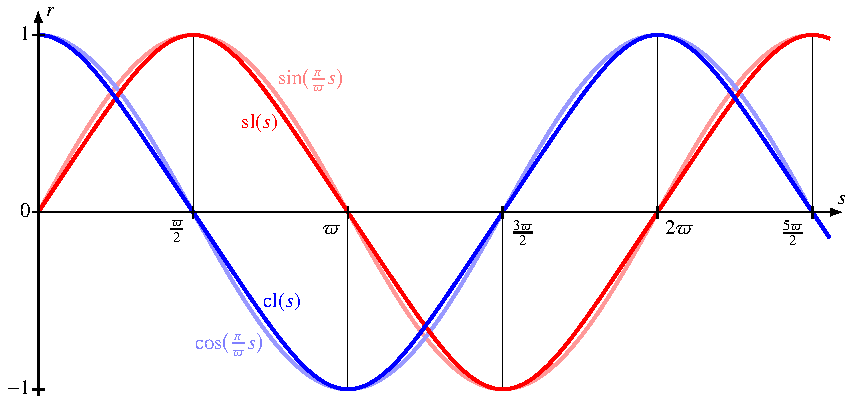
\includegraphics{chapters/110-elliptisch/images/slcl.pdf}
\caption{
Lemniskatischer Sinus und Kosinus sowie Sinus und Kosinus
mit derart skaliertem Argument, dass die Funktionen die gleichen Nullstellen
haben.
\label{buch:elliptisch:figure:slcl}}
\end{figure}


%\section*{Übungsaufgaben}
%\rhead{Übungsaufgaben}
%\aufgabetoplevel{chapters/020-exponential/uebungsaufgaben}
%\begin{uebungsaufgaben}
%\uebungsaufgabe{0}
%\uebungsaufgabe{1}
%\end{uebungsaufgaben}


%%
% chapter.tex -- Beschreibung des Inhaltes
%
% (c) 2021 Prof Dr Andreas Müller, Hochschule Rapperswil
%
% !TeX spellcheck = de_CH
\chapter{Elliptische Funktionen
\label{buch:chapter:geometrie}}
\lhead{Elliptische Funktionen}
\rhead{}

Der Versuch, die Länge eines Ellipsenbogens zu berechnen, hat
in Abschnitt~\ref{buch:geometrie:subsection:hyperbeln-und-ellipsen}
zu Integralen geführt, die nicht in geschlossener Form ausgewertet
werden können.
Neben den dort gefundenen Integralen sind noch weitere, ähnlich
aufgebaute Integrale in dieser Familie zu finden.

%
% ellintegral.tex
%
% (c) 2021 Prof Dr Andreas Müller, OST Ostschweizer Fachhochschule
%
\section{Elliptische Integrale
\label{buch:elliptisch:section:integral}}
\rhead{Elliptisches Integral}
Bei der Berechnung des Ellipsenbogens in 
Abschnitt~\ref{buch:geometrie:subsection:hyperbeln-und-ellipsen}
sind wir auf ein Integral gestossen, welches sich nicht in geschlossener
Form ausdrücken liess.
Um solche Integrale in den Griff zu bekommen, ist es nötig, sie als
neue spezielle Funktionen zu definieren.

\subsection{Definition
\label{buch:elliptisch:subsection:definition}}
Ein {\em elliptisches Integral} ist ein Integral der Form
\index{elliptishes Integral}%
\index{Integral, elliptisch}%
\begin{equation}
\int R\left( x, \sqrt{p(x)}\right)\,dx
\label{buch:elliptisch:def:allgemein}
\end{equation}
wobei $R(x,y)$ eine rationale Funktion von zwei Variablen ist und
$p(x)$ ein Polynom dritten oder vierten Grades.
Hätte $p(x)$ ein mehrfache Nullstelle $x_0$, müsste es durch $(x-x_0)^2$
teilbar sein, man könnte also einen Faktor $(x-x_0)$ aus der
Wurzel im Integraneden von \eqref{buch:elliptisch:def:allgemein}
ausklammern und damit das Integral in eine Form bringen, wo $p(x)$
höchstens zweiten Grades ist.
Solche Integrale lassen sich meistens mit trigonometrischen Substitutionen
berechnen.
Wir verlangen daher, dass $p(x)$ keine mehrfachen Nullstellen hat.

Man kann zeigen, dass sich elliptische Integrale in Summen von
elementaren Funktionen und speziellen elliptischen Integralen 
der folgenden Form überführen lassen
\cite[Abschnitt 164, p.~506]{buch:smirnov32}.

\begin{definition}
\label{buch:elliptisch:def:integrale123}
Die elliptischen Integrale erster, zweiter und dritter Art sind die
Integrale
\[
\begin{aligned}
\text{1.~Art:}&&&
\int \frac{dx}{\sqrt{(1-x^2)(1-k^2x^2)}}
\\
\text{2.~Art:}&&&
\int \sqrt{\frac{1-k^2x^2}{1-x^2}}\,dx
\\
\text{3.~Art:}&&&
\int \frac{dx}{(1-nx^2)\sqrt{(1-x^2)(1-k^2x^2)}}
\end{aligned}
\]
mit $0<k<1$.
Es ist auch üblich, den Parameter $m=k^2$ zu verwenden.
\end{definition}

Wie gesagt lassen sich für diese unbestimmten Integrale keine 
geschlossenen Formen finden.
Es bleibt uns daher nichts anderes übrig, als die Integralgrenzen
festzulegen und damit eine Stammfunktion auszuwählen.

%
% Elliptisches Integral
%
\subsection{Vollständige elliptische Integrale
\label{buch:elliptisch:subsection:vollstaendig}}
In diesem Abschnitt legen wir beide Integrationsgrenzen fest und
untersuchen die entstehenenden Funktionen von den Parametern
$k$ und $n$.

\subsubsection{Definition der vollständigen elliptischen Integrale}
Da der Nenner in allen drei elliptischen Integralen eine Nullstelle
bei $\pm1$ hat, kann das Integral nur von $0$ bis $1$ erstreckt werden.

\begin{definition}
\label{buch:elliptisch:def:vollstintegrale123}
Die vollständigen elliptischen Integrale erster, zweiter und dritter
Art sind
\[
\begin{aligned}
\text{1.~Art:}&&
K(k)&=\int_0^1 \frac{dt}{\sqrt{(1-t^2)(1-k^2t^2)}} \\
\text{2.~Art:}&&
E(k)&=\int_0^1 \sqrt{\frac{1-k^2t^2}{1-t^2}}\,dt \\
\text{3.~Art:}&&
\Pi(n, k)&=\int_0^1\frac{dt}{(1-nt^2)\sqrt{(1-t^2)(1-k^2t^2)}} 
\end{aligned}
\]
mit $0<k<1$.
\end{definition}

Die Funktionen hängen stetig von $k$ ab.
Die Nullstellen des Faktors $1-k^2x^2$ liegen ausserhalb des
Integrationsintervalls und spielen daher keine Rolle.
Die Werte von $K(k)$ und $E(k)$ für $k=0$ können direkt berechnet
werden:
\begin{align*}
K(0)
=
E(0)
&=
\int_0^1 \frac{dt}{\sqrt{1-t^2}}=\frac{\pi}2.
\end{align*}
Das Integral $\Pi(n,0)$ ist etwas komplizierter.

Für $k\to 1$ ist $E(k)=1$, die Integrale $K(1)$ und $\Pi(n,1)$
sind dagegen divergent.

\subsubsection{Jacobi- und Legendre-Normalform}
Die Integrationsvariable $t$ der vollständigen elliptischen Integrale
kann durch die Substitution $t=\sin\varphi$ durch die Variable
$\varphi$ und das Integral über das Intervall $[0,1]$ durch ein
Integral über das Intervall $[0,\frac{\pi}2]$ ersetzt werden.
Mit
\[
\frac{dt}{d\varphi} = \cos\varphi = \sqrt{1-\sin^2\varphi}
\]
können die Funktionen $K(k)$, $E(k)$ und $\Pi(n,k)$ auch als
\begin{align*}
K(k)
&=
\int_0^{\frac{\pi}2}
\frac{
\sqrt{1-\sin^2\varphi}\,d\varphi
}{
\sqrt{(1-\sin^2\varphi)(1-k^2\sin^2\varphi)}
}
=
\int_0^{\frac{\pi}2}
\frac{d\varphi}{\sqrt{1-k^2\sin^2\varphi}}
\\
E(k)
&=
\int_0^{\frac{\pi}2}
\sqrt{\frac{1-k^2\sin^2\varphi}{1-\sin^2\varphi}}\sqrt{1-\sin^2\varphi}\,d\varphi
=
\int_0^{\frac{\pi}2}
\sqrt{1-k^2\sin^2\varphi}\,d\varphi
\\
\Pi(n,k)
&=
\int_0^{\frac{\pi}2}
\frac{
\sqrt{1-\sin^2\varphi}\,d\varphi
}{
(1-n\sin^2\varphi)\sqrt{(1-\sin^2\varphi)(1-k^2\sin^2\varphi)}
}
=
\int_0^{\frac{\pi}2}
\frac{
d\varphi
}{
(1-n\sin^2\varphi)\sqrt{1-k^2\sin^2\varphi}
}
\end{align*}
Diese Form wird auch die {\em Legendre-Normalform} der vollständigen 
\index{Legendre-Normalform}%
elliptischen Integrale genannt, während die Form von
Definition~\ref{buch:elliptisch:def:vollstintegrale123}
die {\em Jacobi-Normalform} heisst.
\index{Jacobi-Normalform}%

\subsubsection{Umfang einer Ellipse}
\begin{figure}
\centering
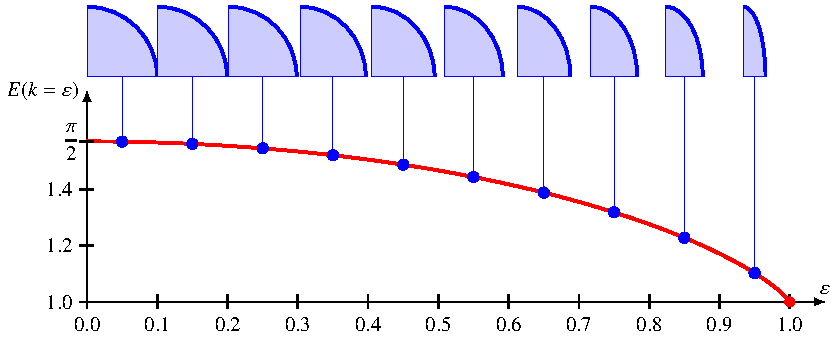
\includegraphics{chapters/110-elliptisch/images/ellipsenumfang.pdf}
\caption{Bogenlänge eines Viertels einer Ellipse mit Exzentrizität
$\varepsilon$.
\label{buch:elliptisch:fig:ellipsenumfang}}
\end{figure}
Wir zeigen, wie sich die Berechnung des Umfangs $U$ einer Ellipse
mit Halbachsen $a$ und $b$, $a\le b$, auf ein volltändiges elliptisches
Integral zurückführen lässt.
Der Fall $a>b$ kann behandelt werden, indem die $x$- und $y$-Koordinaten
vertauscht werden.

Die Parametrisierung
\[
t\mapsto \begin{pmatrix}a\cos t\\ b\sin t\end{pmatrix}
\]
einer Ellipse führt auf das Integral
\begin{align*}
U
&=
\int_0^{2\pi} \sqrt{a^2\sin^2t + b^2\cos^2 t}\,dt
\notag
\\
&=
4\int_0^{\frac{\pi}2}
\sqrt{a^2\sin^2t + b^2(1-\sin^2 t)}
\,dt
\notag
\\
&=
4b \int_0^{\frac{\pi}2} \sqrt{1-(b^2-a^2)/b^2\cdot \sin^2t}\,dt
\label{buch:elliptisch:eqn:umfangellipse}
\end{align*}
für den Umfang der Ellipse.
Bei einem Kreis ist $a=b$ und der zweite Term unter der Wurzel fällt weg,
der Umfang wird $4b\frac{\pi}2=2\pi b$.
Die Differenz $e^2=b^2-a^2$ ist die {\em lineare Exzentrizität} der Ellipse,
\index{lineare Exzentrizität}%
der Quotient $e/b$ wird die {\em numerische Exzentrizität} der Ellipse
genannt.
Insbesondere ist $k = \varepsilon$.

Das Integral~\eqref{buch:elliptisch:eqn:umfangellipse} erhält jetzt die
Form
\[
U
=
4b\int_0^{\frac{\pi}2} \sqrt{1-k^2\sin^2t}\,dt
\]
und ist damit als elliptisches Integral zweiter Art erkannt.
Für den Umfang der Ellipse finden wir damit die Formel
\[
U
=
4b E(k)
=
4b E(\varepsilon).
\]
Das vollständige elliptische Integral zweiter Art $E(\varepsilon)$
liefert also genau den Umfang der eines Viertels Ellipse mit
numerischer Exzentrizität $\varepsilon$ und kleiner Halbachse $1$.

\subsubsection{Komplementäre Integrale}
XXX Komplementäre Integrale \\

\subsubsection{Ableitung}
XXX Ableitung \\
XXX Stammfunktion \\

\subsection{Unvollständige elliptische Integrale}
XXX Vollständige und Unvollständige Integrale \\
XXX Additionstheoreme \\
XXX Parameterkonventionen \\

\subsection{Potenzreihe}
XXX Potenzreihen \\
XXX Als hypergeometrische Funktionen \\



\section{Jacobische elliptische Funktionen}

Für das elliptische Filter werden, wie es der Name bereits deutet, elliptische Funktionen gebraucht.
Wie die trigonometrischen Funktionen Zusammenhänge eines Kreises darlegen, beschreiben die elliptischen Funktionen Ellipsen.
Es ist daher naheliegend, dass der Kosinus des Tschebyscheff-Filters gegen ein elliptisches Pendant ausgetauscht werden könnte.
Der Begriff elliptische Funktion wird für sehr viele Funktionen gebraucht, daher ist es hier wichtig zu erwähnen, dass es ausschliesslich um die Jacobischen elliptischen Funktionen geht.

\subsection{Grundlegende Eigenschaften}

Die Jacobi elliptischen Funktionen werden ausführlich im Kapitel \ref{buch:elliptisch:section:jacobi} behandelt.
Im Wesentlichen erweitern die Jacobi elliptischen Funktionen die trigonometrische Funktionen für Ellipsen.
Zum Beispiel gibt es analog zum Sinus den elliptischen $\sn(z, k)$.
Im Gegensatz zum den trigonometrischen Funktionen haben die elliptischen Funktionen zwei Parameter.
Den \textit{elliptische Modul} $k$, der die Exzentrizität der Ellipse parametrisiert und das Winkelargument $z$.
Im Kreis ist der Radius für alle Winkel konstant, bei Ellipsen ändert sich das.
Dies hat zur Folge, dass bei einer Ellipse die Kreisbogenlänge nicht linear zum Winkel verläuft.
Darum kann hier nicht der gewohnte Winkel verwendet werden.
Das Winkelargument $z$ kann durch das elliptische Integral erster Art
\begin{equation}
    z
    =
    F(\phi, k)
    =
    \int_{0}^{\phi}
    \frac{
        d\theta
    }{
        \sqrt{
            1-k^2 \sin^2 \theta
        }
    }
\end{equation}
mit dem Winkel $\phi$ in Verbindung gebracht werden.

Dabei wird das vollständige und unvollständige elliptische integral unterschieden.
Beim vollständigen Integral
\begin{equation}
    K(k)
    =
    \int_{0}^{\pi / 2}
    \frac{
        d\theta
    }{
        \sqrt{
            1-k^2 \sin^2 \theta
        }
    }
\end{equation}
wird über ein viertel Ellipsenbogen integriert, also bis $\phi=\pi/2$ und liefert das Winkelargument für eine Vierteldrehung.
Die Zahl wird oft auch abgekürzt mit $K = K(k)$ und ist für das elliptische Filter sehr relevant.
Alle elliptischen Funktionen sind somit $4K$-periodisch.

Neben dem $\sn$ gibt es zwei weitere elliptische Basisfunktionen $\cn$ und $\dn$.
Dazu kommen noch weitere abgeleitete Funktionen, die durch Quotienten und Kehrwerte dieser Funktionen zustande kommen.
Insgesamt sind es die zwölf Funktionen
\begin{equation*}
    \sn \quad
    \ns \quad
    \scelliptic \quad
    \sd \quad
    \cn \quad
    \nc \quad
    \cs \quad
    \cd \quad
    \dn \quad
    \nd \quad
    \ds \quad
    \dc.
\end{equation*}

Die Jacobischen elliptischen Funktionen können mit der inversen Funktion des vollständigen elliptischen Integrals erster Art
\begin{equation}
    \phi = F^{-1}(z, k)
\end{equation}
definiert werden. Dabei ist zu beachten dass nur das $z$ Argument der Funktion invertiert wird, also
\begin{equation}
    z = F(\phi, k)
    \Leftrightarrow
    \phi = F^{-1}(z, k).
\end{equation}
Mithilfe von $F^{-1}$ kann zum Beispiel $sn^{-1}$ mit dem elliptischen Integral dargestellt werden:
\begin{equation}
    \sin(\phi)
    =
    \sin \left( F^{-1}(z, k) \right)
    =
    \sn(z, k)
    =
    w.
\end{equation}

% \begin{equation} %TODO remove unnecessary equations
%     \phi
%     =
%      F^{-1}(z, k)
%      =
%      \sin^{-1} \big( \sn (z, k ) \big)
%      =
%     \sin^{-1} ( w )
% \end{equation}

% \begin{equation}
%     F(\phi, k)
%     =
%     z
%     =
%     F( \sin^{-1} \big( \sn (z, k ) \big) , k)
%     =
%     F( \sin^{-1} ( w ), k)
% \end{equation}

% \begin{equation}
%     \sn^{-1}(w, k)
%     =
%     F(\phi, k),
%     \quad
%     \phi = \sin^{-1}(w)
% \end{equation}

\subsection{Die Funktion $\sn^{-1}$}

Beim Tschebyscheff-Filter konnten wir mit Betrachten des Arcuscosinus die Funktionalität erklären.
Für das Elliptische Filter machen wir die gleiche Betrachtung mit der $\sn^{-1}$-Funktion.
Der $\sn^{-1}$ ist durch das elliptische Integral
\begin{align}
    \sn^{-1}(w, k)
        & =
    \int_{0}^{\phi}
    \frac{
        d\theta
    }{
        \sqrt{
            1-k^2 \sin^2 \theta
        }
    },
    \quad
    \phi = \sin^{-1}(w)
    \\
        & =
    \int_{0}^{w}
    \frac{
        dt
    }{
        \sqrt{
            (1-t^2)(1-k^2 t^2)
        }
    }
\end{align}
beschrieben.
Dazu betrachten wir wieder den Integranden
\begin{equation}
    \frac{
        1
    }{
        \sqrt{
            (1-t^2)(1-k^2 t^2)
        }
    }.
\end{equation}
Beim $\cos^{-1}(x)$ haben wir gesehen, dass die analytische Fortsetzung bei $x < -1$ und $x > 1$ rechtwinklig in die komplexen Zahlen wandert.
Wenn man das Gleiche mit $\sn^{-1}(w, k)$ macht, erkennt man zwei interessante Stellen.
Die erste ist die gleiche wie beim $\cos^{-1}(x)$ nämlich bei $t = \pm 1$.
Der erste Term unter der Wurzel wird dann negativ, während der zweite noch positiv ist, da $k \leq 1$.
Ab diesem Punkt knickt die Funktion in die imaginäre Richtung ab.
Bei $t = 1/k$ ist auch der zweite Term negativ und die Funktion verläuft in die negative reelle Richtung.
Abbildung \ref{ellfilter:fig:sn} zeigt den Verlauf der Funktion in der komplexen Ebene.
\begin{figure}
    \centering
    \begin{tikzpicture}[>=stealth', auto, node distance=2cm, scale=1.2]

    \tikzstyle{zero} = [draw, circle, inner sep =0, minimum height=0.15cm]

    \tikzset{pole/.style={cross out, draw=black, minimum size=(0.15cm-\pgflinewidth), inner sep=0pt, outer sep=0pt}}

    \begin{scope}[xscale=0.9, yscale=1.8]

        \draw[gray, ->] (0,-1.5) -- (0,1.5) node[anchor=south]{$\mathrm{Im}~z$};
        \draw[gray, ->] (-5,0) -- (5,0) node[anchor=west]{$\mathrm{Re}~z$};

        \begin{scope}

            \clip(-4.5,-1.25) rectangle (4.5,1.25);

            \fill[yellow!30] (0,0) rectangle (1, 0.5);

            \begin{scope}[xshift=-1cm]

                \foreach \i in {-2,...,2} {
                    \foreach \j in {-2,...,1} {
                        \begin{scope}[xshift=\i*4cm, yshift=\j*1cm]
                            \draw[<-, blue!50] (0, 0) -- (0,0.5);
                            \draw[<-, cyan!50] (1, 0) -- (0,0);
                            \draw[<-, darkgreen!50] (2, 0) -- (1,0);
                            \draw[<-, orange!50] (2,0.5) -- (2, 0);
                            \draw[<-, red!50] (1, 0.5) -- (2,0.5);
                            \draw[<-, purple!50] (0, 0.5) -- (1,0.5);
                            \draw[<-, blue!50] (0,1) -- (0,0.5);
                            \draw[<-, orange!50] (2,0.5) -- (2, 1);
                            \draw[<-, red!50] (3, 0.5) -- (2,0.5);
                            \draw[<-, purple!50] (4, 0.5) -- (3,0.5);
                            \draw[<-, darkgreen!50] (2, 0) -- (3,0);
                            \draw[<-, cyan!50] (3, 0) -- (4,0);
                        \end{scope}
                    }
                }

                % \pause
                \draw[ultra thick, <-, darkgreen] (2, 0) -- (1,0);
                % \pause
                \draw[ultra thick, <-, orange] (2,0.5) -- (2, 0);
                % \pause
                \draw[ultra thick, <-, red] (1, 0.5) -- (2,0.5);
                % \pause
                \draw[ultra thick, <-, blue] (0, 0) -- (0,0.5);
                \draw[ultra thick, <-, purple] (0, 0.5) -- (1,0.5);
                \draw[ultra thick, <-, cyan] (1, 0) -- (0,0);
                % \pause


                \foreach \i in {-2,...,2} {
                    \foreach \j in {-2,...,1} {
                        \begin{scope}[xshift=\i*4cm, yshift=\j*1cm]
                            \node[zero] at ( 1, 0) {};
                            \node[zero] at ( 3, 0) {};
                            \node[pole] at ( 1,0.5) {};
                            \node[pole] at ( 3,0.5) {};
                        \end{scope}
                    }
                }

            \end{scope}

        \end{scope}

        \draw[gray] ( 1,0) +(0,0.1) -- +(0, -0.1) node[inner sep=0, anchor=north] {\small $K$};
        \draw[gray]  (0, 0.5) +(0.1, 0) -- +(-0.1, 0) node[inner sep=0, anchor=east]{\small $jK^\prime$};

    \end{scope}

    \node[zero] at (4,3) (n) {};
    \node[anchor=west] at (n.east) {Zero};
    \node[pole, below=0.25cm of n] (n) {};
    \node[anchor=west] at (n.east) {Pole};

    \begin{scope}[yshift=-4cm, xscale=0.75]

        \draw[gray, ->] (-6,0) -- (6,0) node[anchor=west]{$w$};

        \draw[ultra thick, ->, purple] (-5, 0) -- (-3, 0);
        \draw[ultra thick, ->, blue]      (-3, 0) -- (-2, 0);
        \draw[ultra thick, ->, cyan]       (-2, 0) -- (0, 0);
        \draw[ultra thick, ->, darkgreen]    (0, 0) -- (2, 0);
        \draw[ultra thick, ->, orange] (2, 0) -- (3, 0);
        \draw[ultra thick, ->, red] (3, 0) -- (5, 0);

        \node[anchor=south] at (-5,0) {$-\infty$};
        \node[anchor=south] at (-3,0) {$-1/k$};
        \node[anchor=south] at (-2,0) {$-1$};
        \node[anchor=south] at (0,0) {$0$};
        \node[anchor=south] at (2,0) {$1$};
        \node[anchor=south] at (3,0) {$1/k$};
        \node[anchor=south] at (5,0) {$\infty$};

    \end{scope}


\end{tikzpicture}
    \caption{
        $z$-Ebene der Funktion $z = \sn^{-1}(w, k)$.
        Die Funktion ist in der realen Achse $4K$-periodisch und in der imaginären Achse $2jK^\prime$-periodisch.
    }
    \label{ellfilter:fig:sn}
\end{figure}
In der reellen Richtung ist sie $4K(k)$-periodisch und in der imaginären Richtung $4K^\prime(k)$-periodisch, wobei $K^\prime$ das komplementäre vollständige Elliptische Integral ist:
\begin{equation}
    K^\prime(k)
    =
    \int_{0}^{\pi / 2}
    \frac{
        d\theta
    }{
        \sqrt{
            1-{k^\prime}^2 \sin^2 \theta
        }
    },
    \quad
    k^\prime = \sqrt{1-k^2}.
\end{equation}

%
% lemniskate.tex
%
% (c) 2021 Prof Dr Andreas Müller, OST Ostschweizer Fachhochschule
%
\section{Lemniskatischer Sinus
\label{buch:elliptisch:section:lemniskate}}
\rhead{Lemniskatischer Sinus}
Historisch war der {\em lemniskatische Sinus} die erste ellptische
Funktion, die Gauss bereits als 19-jähriger untersucht, aber nicht 
veröffentlich hat.
In diesem Abschnitt soll die Verbindung zu den Jacobischen
elliptischen Funktionen hergestellt werden.

\subsection{Lemniskate
\label{buch:gemotrie:subsection:lemniskate}}
\begin{figure}
\centering
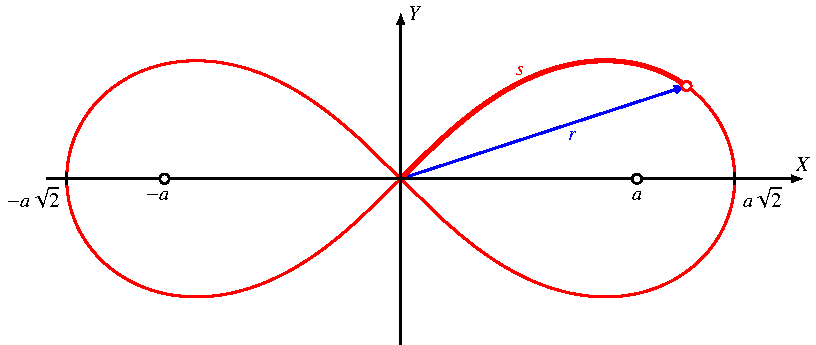
\includegraphics{chapters/110-elliptisch/images/lemniskate.pdf}
\caption{Bogenlänge und Radius der Lemniskate von Bernoulli.
\label{buch:elliptisch:fig:lemniskate}}
\end{figure}
Die Lemniskate von Bernoulli ist die Kurve vierten Grades mit der Gleichung
\begin{equation}
(X^2+Y^2)^2 = 2a^2(X^2-Y^2).
\label{buch:elliptisch:eqn:lemniskate}
\end{equation}
Sie ist in Abbildung~\ref{buch:elliptisch:fig:lemniskate}
dargestellt.
Die beiden Scheitel der Lemniskate befinden sich bei $X_s=\pm a\sqrt{2}$.
Dividiert man die Gleichung der Lemniskate durch $X_s^2=4a^4$ entsteht 
\begin{equation}
\biggl(
\biggl(\frac{X}{a\sqrt{2}}\biggr)^2
+
\biggl(\frac{Y}{a\sqrt{2}}\biggr)^2
\biggr)^2
=
2\frac{a^2}{2a^2}\biggl(
\biggl(\frac{X}{a\sqrt{2}}\biggr)^2
-
\biggl(\frac{Y}{a\sqrt{2}}\biggr)^2
\biggr).
\qquad
\Leftrightarrow
\qquad
(x^2+y^2)^2 = x^2-y^2,
\label{buch:elliptisch:eqn:lemniskatenormiert}
\end{equation}
wobei wir $x=X/a\sqrt{2}$ und $y=Y/a\sqrt{2}$ gesetzt haben.
In dieser Normierung liegen die Scheitel bei $\pm 1$.
Dies ist die Skalierung, die für die Definition des lemniskatischen
Sinus und Kosinus verwendet werden soll.

In Polarkoordinaten $x=r\cos\varphi$ und $y=r\sin\varphi$
gilt nach Einsetzen in \eqref{buch:elliptisch:eqn:lemniskatenormiert}
\begin{equation}
r^4
=
r^2(\cos^2\varphi-\sin^2\varphi)
=
r^2\cos2\varphi
\qquad\Rightarrow\qquad
r^2 = \cos 2\varphi
\label{buch:elliptisch:eqn:lemniskatepolar}
\end{equation}
als Darstellung der Lemniskate in Polardarstellung.
Sie gilt für Winkel $\varphi\in[-\frac{\pi}4,\frac{\pi}4]$ für das
rechte Blatt und $\varphi\in[\frac{3\pi}4,\frac{5\pi}4]$ für das linke
Blatt der Lemniskate.

\subsection{Bogenlänge}
Die Funktionen
\begin{equation}
x(r) = \frac{r}{\sqrt{2}}\sqrt{1+r^2},
\quad
y(r) = \frac{r}{\sqrt{2}}\sqrt{1-r^2}
\label{buch:geometrie:eqn:lemniskateparam}
\end{equation}
erfüllen
\begin{align*}
x(r)^2-y(r)^2
&=
\frac{r^2(1+r^2)}{2}-\frac{r^2(1-r^2)}{2}
\\
&
=
r^4
=
(x(r)^2 + y(r)^2)^2,
\end{align*}
sie stellen also eine Parametrisierung der Lemniskate dar.

Mit Hilfe der Parametrisierung~\eqref{buch:geometrie:eqn:lemniskateparam}
kann man die Länge $s$ des in Abbildung~\ref{buch:elliptisch:fig:lemniskate}
dargestellten Bogens der Lemniskate berechnen.
Dazu benötigt man die Ableitungen nach $r$, die man mit der Produkt- und
Kettenregel berechnen kann:
\begin{align*}
\dot{x}(r)
&=
\frac{\sqrt{1+r^2}}{\sqrt{2}}
+
\frac{r^2}{\sqrt{2}\sqrt{1+r^2}}
&&\Rightarrow&
\dot{x}(r)^2
&=
\frac{1+r^2}{2} +r^2 + \frac{r^4}{2(1+r^2)}
\\
\dot{y}(r)
&=
\frac{\sqrt{1-r^2}}{\sqrt{2}}
-
\frac{r^2}{\sqrt{2}\sqrt{1-r^2}}
&&\Rightarrow&
\dot{y}(r)^2
&=
\frac{1-r^2}{2} -r^2 + \frac{r^4}{2(1-r^2)}
\end{align*}
Die Summe der Quadrate ist
\begin{align*}
\dot{x}(r)^2 + \dot{y}(r)^2
&=
1 + r^4\frac{1-r^2+1+r^2}{2(1+r^2)(1-r^2)}
=
1+r^4\frac{2}{2(1-r^4)}
=
\frac{1-r^4+r^4}{1-r^4}
=
\frac1{1-r^4}.
\end{align*}
Durch Einsetzen in das Integral für die Bogenlänge bekommt man
\begin{equation}
s(r)
=
\int_0^r
\frac{1}{\sqrt{1-t^4}}\,dt.
\label{buch:elliptisch:eqn:lemniskatebogenlaenge}
\end{equation}

%
% Als elliptisches Integral
%
\subsection{Darstellung als elliptisches Integral}
Das unvollständige elliptische Integral erster Art mit Parameter
$k^2=-1$ oder $k=i$ ist
\[
K(r,i)
=
\int_0^x \frac{dt}{\sqrt{(1-t^2)(1-i^2 t^2)}}
=
\int_0^x \frac{dt}{\sqrt{(1-t^2)(1-(-1)t^2)}}
=
\int_0^x \frac{dt}{\sqrt{1-t^4}}
=
s(r).
\]
Der lemniskatische Sinus ist also eine Umkehrfunktion des
elliptischen Integrals erster Art für den speziellen Wert $i$ des
Parameters $k$.

Die Länge des rechten Blattes der Lemniskate wird mit $\varpi$ bezeichnet
und hat den numerischen Wert
\[
\varpi
=
2\int_0^1\sqrt{\frac{1}{1-t^4}}\,dt
=
2.6220575542.
\]
$\varpi$ ist auch als die {\em lemniskatische Konstante} bekannt.
\index{lemniskatische Konstante}%
Der Lemniskatenbogen zwischen dem Nullpunkt und $(1,0)$ hat die Länge
$\varpi/2$.

%
%  Bogenlängenparametrisierung
%
\subsection{Bogenlängenparametrisierung}
Die Lemniskate mit der Gleichung
\[
(X^2+X^2)^2=2(X^2-X^2)
\]
(der Fall $a=1$ in \eqref{buch:elliptisch:eqn:lemniskate})
kann mit Jacobischen elliptischen Funktionen
parametrisiert werden.
Dazu schreibt man
\[
\left.
\begin{aligned}
X(t)
&=
\sqrt{2}\operatorname{cn}(t,k) \operatorname{dn}(t,k)
\\
Y(t)
&=
\phantom{\sqrt{2}}
\operatorname{cn}(t,k) \operatorname{sn}(t,k)
\end{aligned}
\quad\right\}
\qquad\text{mit $k=\displaystyle\frac{1}{\sqrt{2}}$}
\]
und berechnet die beiden Seiten der definierenden Gleichung der
Lemniskate.
Zunächst ist
\begin{align*}
X(t)^2
&=
2\operatorname{cn}(t,k)^2
\operatorname{dn}(t,k)^2
\\
Y(t)^2
&=
\operatorname{cn}(t,k)^2
\operatorname{sn}(t,k)^2
\\
X(t)^2+Y(t)^2
&=
2\operatorname{cn}(t,k)^2
\bigl(
\underbrace{
\operatorname{dn}(t,k)^2
+{\textstyle\frac12}
\operatorname{sn}(t,k)^2
}_{\displaystyle =1}
\bigr)
%\\
%&
=
2\operatorname{cn}(t,k)^2
\\
X(t)^2-Y(t)^2
&=
\operatorname{cn}(t,k)^2
\bigl(
2\operatorname{dn}(t,k)^2 - \operatorname{sn}(t,k)^2
\bigr)
\\
&=
\operatorname{cn}(t,k)^2
\bigl(
2\bigl({\textstyle\frac12}+{\textstyle\frac12}\operatorname{cn}(t,k)^2\bigr)
-
\bigl(1-\operatorname{cn}(t,k)^2\bigr)
\bigr)
\\
&=
2\operatorname{cn}(t,k)^4
\\
\Rightarrow\qquad
(X(t)^2+Y(t)^2)^2
&=
4\operatorname{cn}(t,k)^4
=
2(X(t)^2-Y(t)^2).
\end{align*}
Wir zeigen jetzt, dass dies tatsächlich eine Bogenlängenparametrisierung
der Lemniskate ist.
Dazu berechnen wir die Ableitungen
\begin{align*}
\dot{X}(t)
&=
\sqrt{2}\operatorname{cn}'(t,k)\operatorname{dn}(t,k)
+
\sqrt{2}\operatorname{cn}(t,k)\operatorname{dn}'(t,k)
\\
&=
-\sqrt{2}\operatorname{sn}(t,k)\operatorname{dn}(t,k)^2
-\frac12\sqrt{2}\operatorname{sn}(t,k)\operatorname{cn}(t,k)^2
\\
&=
-\sqrt{2}\operatorname{sn}(t,k)\bigl(
1-{\textstyle\frac12}\operatorname{sn}(t,k)^2
+{\textstyle\frac12}-{\textstyle\frac12}\operatorname{sn}(u,t)^2
\bigr)
\\
&=
\sqrt{2}\operatorname{sn}(t,k)
\bigl(
{\textstyle \frac32}-\operatorname{sn}(t,k)^2
\bigr)
\\
\dot{X}(t)^2
&=
2\operatorname{sn}(t,k)^2
\bigl(
{\textstyle \frac32}-\operatorname{sn}(t,k)^2
\bigr)^2
\\
&=
{\textstyle\frac{9}{2}}\operatorname{sn}(t,k)^2
-
6\operatorname{sn}(t,k)^4
+2\operatorname{sn}(t,k)^6
\\
\dot{Y}(t)
&=
\operatorname{cn}'(t,k)\operatorname{sn}(t,k)
+
\operatorname{cn}(t,k)\operatorname{sn}'(t,k)
\\
&=
-\operatorname{sn}(t,k)^2
\operatorname{dn}(t,k)
+\operatorname{cn}(t,k)^2
\operatorname{dn}(t,k)
\\
&=
\operatorname{dn}(t,k)\bigl(1-2\operatorname{sn}(t,k)^2\bigr)
\\
\dot{Y}(t)^2
&=
\bigl(1-{\textstyle\frac12}\operatorname{sn}(t,k)^2\bigr)
\bigl(1-2\operatorname|{sn}(t,k)^2\bigr)^2
\\
&=
1-{\textstyle\frac{9}{2}}\operatorname{sn}(t,k)^2
+6\operatorname{sn}(t,k)^4
-2\operatorname{sn}(t,k)^6
\\
\dot{X}(t)^2 + \dot{Y}(t)^2
&=
1.
\end{align*}
Dies bedeutet, dass die Bogenlänge zwischen den Parameterwerten $0$ und $s$
\[
\int_0^s
\sqrt{\dot{X}(t)^2 + \dot{Y}(t)^2}
\,dt
=
\int_0^s\,dt
=
s,
\]
der Parameter $t$ ist also ein Bogenlängenparameter.

Die mit dem Faktor $1/\sqrt{2}$ skalierte Standard-Lemniskate mit der
Gleichung
\[
(x^2+y^2)^2 = x^2-y^2
\]
hat daher eine Bogenlängenparametrisierung mit
\begin{equation}
\begin{aligned}
x(t)
&=
\phantom{\frac{1}{\sqrt{2}}}
\operatorname{cn}(\sqrt{2}t,k)\operatorname{dn}(\sqrt{2}t,k)
\\
y(t)
&=
\frac{1}{\sqrt{2}}\operatorname{cn}(\sqrt{2}t,k)\operatorname{sn}(\sqrt{2}t,k)
\end{aligned}
\label{buch:elliptisch:lemniskate:bogenlaenge}
\end{equation}

\subsection{Der lemniskatische Sinus und Kosinus}
Der Sinus Berechnet die Gegenkathete zu einer gegebenen Bogenlänge des
Kreises, er ist die Umkehrfunktion der Funktion, die der Gegenkathete
die Bogenlänge zuordnet.

Daher ist es naheliegend, die Umkehrfunktion von $s(r)$ in 
\eqref{buch:elliptisch:eqn:lemniskatebogenlaenge}
den {\em lemniskatischen Sinus} zu nennen mit der Bezeichnung
$r=\operatorname{sl} s$.

Der Kosinus ist der Sinus des komplementären Winkels.
Auch für die lemniskatische Bogenlänge $s(r)$ lässt sich eine
komplementäre Bogenlänge definieren, nämlich die Bogenlänge zwischen
dem Punkt $(x(r), y(r))$ und $(1,0)$.

Da die Parametrisierung~\eqref{buch:elliptisch:lemniskate:bogenlaenge}
eine Bogenlängenparametrisierung ist, darf man $t=s$ schreiben.
Dann kann man aber auch $r(s)$ daraus berechnen,
es ist
\[
r(s)^2
=
x(s)^2 + y(s)^2
=
\operatorname{cn}(s\sqrt{2},k)^2
\qquad\Rightarrow\qquad
r(s)
=
\operatorname{cn}(s\sqrt{2},k)
\]

\begin{figure}
\centering
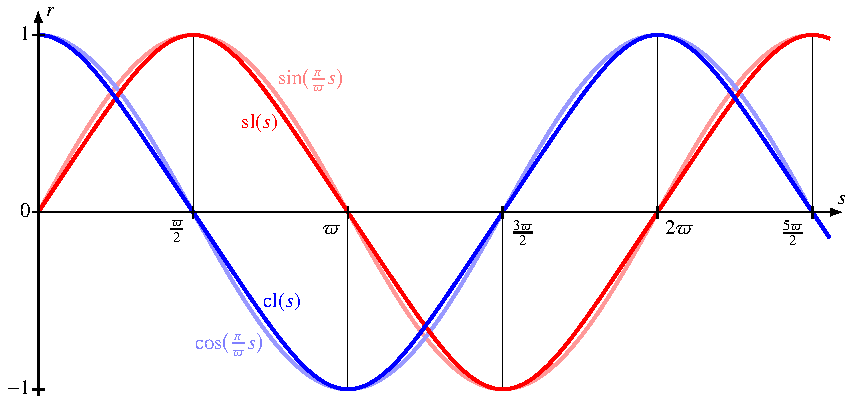
\includegraphics{chapters/110-elliptisch/images/slcl.pdf}
\caption{
Lemniskatischer Sinus und Kosinus sowie Sinus und Kosinus
mit derart skaliertem Argument, dass die Funktionen die gleichen Nullstellen
haben.
\label{buch:elliptisch:figure:slcl}}
\end{figure}


%\section*{Übungsaufgaben}
%\rhead{Übungsaufgaben}
%\aufgabetoplevel{chapters/020-exponential/uebungsaufgaben}
%\begin{uebungsaufgaben}
%\uebungsaufgabe{0}
%\uebungsaufgabe{1}
%\end{uebungsaufgaben}


%%
% chapter.tex -- Beschreibung des Inhaltes
%
% (c) 2021 Prof Dr Andreas Müller, Hochschule Rapperswil
%
% !TeX spellcheck = de_CH
\chapter{Elliptische Funktionen
\label{buch:chapter:geometrie}}
\lhead{Elliptische Funktionen}
\rhead{}

Der Versuch, die Länge eines Ellipsenbogens zu berechnen, hat
in Abschnitt~\ref{buch:geometrie:subsection:hyperbeln-und-ellipsen}
zu Integralen geführt, die nicht in geschlossener Form ausgewertet
werden können.
Neben den dort gefundenen Integralen sind noch weitere, ähnlich
aufgebaute Integrale in dieser Familie zu finden.

%
% ellintegral.tex
%
% (c) 2021 Prof Dr Andreas Müller, OST Ostschweizer Fachhochschule
%
\section{Elliptische Integrale
\label{buch:elliptisch:section:integral}}
\rhead{Elliptisches Integral}
Bei der Berechnung des Ellipsenbogens in 
Abschnitt~\ref{buch:geometrie:subsection:hyperbeln-und-ellipsen}
sind wir auf ein Integral gestossen, welches sich nicht in geschlossener
Form ausdrücken liess.
Um solche Integrale in den Griff zu bekommen, ist es nötig, sie als
neue spezielle Funktionen zu definieren.

\subsection{Definition
\label{buch:elliptisch:subsection:definition}}
Ein {\em elliptisches Integral} ist ein Integral der Form
\index{elliptishes Integral}%
\index{Integral, elliptisch}%
\begin{equation}
\int R\left( x, \sqrt{p(x)}\right)\,dx
\label{buch:elliptisch:def:allgemein}
\end{equation}
wobei $R(x,y)$ eine rationale Funktion von zwei Variablen ist und
$p(x)$ ein Polynom dritten oder vierten Grades.
Hätte $p(x)$ ein mehrfache Nullstelle $x_0$, müsste es durch $(x-x_0)^2$
teilbar sein, man könnte also einen Faktor $(x-x_0)$ aus der
Wurzel im Integraneden von \eqref{buch:elliptisch:def:allgemein}
ausklammern und damit das Integral in eine Form bringen, wo $p(x)$
höchstens zweiten Grades ist.
Solche Integrale lassen sich meistens mit trigonometrischen Substitutionen
berechnen.
Wir verlangen daher, dass $p(x)$ keine mehrfachen Nullstellen hat.

Man kann zeigen, dass sich elliptische Integrale in Summen von
elementaren Funktionen und speziellen elliptischen Integralen 
der folgenden Form überführen lassen
\cite[Abschnitt 164, p.~506]{buch:smirnov32}.

\begin{definition}
\label{buch:elliptisch:def:integrale123}
Die elliptischen Integrale erster, zweiter und dritter Art sind die
Integrale
\[
\begin{aligned}
\text{1.~Art:}&&&
\int \frac{dx}{\sqrt{(1-x^2)(1-k^2x^2)}}
\\
\text{2.~Art:}&&&
\int \sqrt{\frac{1-k^2x^2}{1-x^2}}\,dx
\\
\text{3.~Art:}&&&
\int \frac{dx}{(1-nx^2)\sqrt{(1-x^2)(1-k^2x^2)}}
\end{aligned}
\]
mit $0<k<1$.
Es ist auch üblich, den Parameter $m=k^2$ zu verwenden.
\end{definition}

Wie gesagt lassen sich für diese unbestimmten Integrale keine 
geschlossenen Formen finden.
Es bleibt uns daher nichts anderes übrig, als die Integralgrenzen
festzulegen und damit eine Stammfunktion auszuwählen.

%
% Elliptisches Integral
%
\subsection{Vollständige elliptische Integrale
\label{buch:elliptisch:subsection:vollstaendig}}
In diesem Abschnitt legen wir beide Integrationsgrenzen fest und
untersuchen die entstehenenden Funktionen von den Parametern
$k$ und $n$.

\subsubsection{Definition der vollständigen elliptischen Integrale}
Da der Nenner in allen drei elliptischen Integralen eine Nullstelle
bei $\pm1$ hat, kann das Integral nur von $0$ bis $1$ erstreckt werden.

\begin{definition}
\label{buch:elliptisch:def:vollstintegrale123}
Die vollständigen elliptischen Integrale erster, zweiter und dritter
Art sind
\[
\begin{aligned}
\text{1.~Art:}&&
K(k)&=\int_0^1 \frac{dt}{\sqrt{(1-t^2)(1-k^2t^2)}} \\
\text{2.~Art:}&&
E(k)&=\int_0^1 \sqrt{\frac{1-k^2t^2}{1-t^2}}\,dt \\
\text{3.~Art:}&&
\Pi(n, k)&=\int_0^1\frac{dt}{(1-nt^2)\sqrt{(1-t^2)(1-k^2t^2)}} 
\end{aligned}
\]
mit $0<k<1$.
\end{definition}

Die Funktionen hängen stetig von $k$ ab.
Die Nullstellen des Faktors $1-k^2x^2$ liegen ausserhalb des
Integrationsintervalls und spielen daher keine Rolle.
Die Werte von $K(k)$ und $E(k)$ für $k=0$ können direkt berechnet
werden:
\begin{align*}
K(0)
=
E(0)
&=
\int_0^1 \frac{dt}{\sqrt{1-t^2}}=\frac{\pi}2.
\end{align*}
Das Integral $\Pi(n,0)$ ist etwas komplizierter.

Für $k\to 1$ ist $E(k)=1$, die Integrale $K(1)$ und $\Pi(n,1)$
sind dagegen divergent.

\subsubsection{Jacobi- und Legendre-Normalform}
Die Integrationsvariable $t$ der vollständigen elliptischen Integrale
kann durch die Substitution $t=\sin\varphi$ durch die Variable
$\varphi$ und das Integral über das Intervall $[0,1]$ durch ein
Integral über das Intervall $[0,\frac{\pi}2]$ ersetzt werden.
Mit
\[
\frac{dt}{d\varphi} = \cos\varphi = \sqrt{1-\sin^2\varphi}
\]
können die Funktionen $K(k)$, $E(k)$ und $\Pi(n,k)$ auch als
\begin{align*}
K(k)
&=
\int_0^{\frac{\pi}2}
\frac{
\sqrt{1-\sin^2\varphi}\,d\varphi
}{
\sqrt{(1-\sin^2\varphi)(1-k^2\sin^2\varphi)}
}
=
\int_0^{\frac{\pi}2}
\frac{d\varphi}{\sqrt{1-k^2\sin^2\varphi}}
\\
E(k)
&=
\int_0^{\frac{\pi}2}
\sqrt{\frac{1-k^2\sin^2\varphi}{1-\sin^2\varphi}}\sqrt{1-\sin^2\varphi}\,d\varphi
=
\int_0^{\frac{\pi}2}
\sqrt{1-k^2\sin^2\varphi}\,d\varphi
\\
\Pi(n,k)
&=
\int_0^{\frac{\pi}2}
\frac{
\sqrt{1-\sin^2\varphi}\,d\varphi
}{
(1-n\sin^2\varphi)\sqrt{(1-\sin^2\varphi)(1-k^2\sin^2\varphi)}
}
=
\int_0^{\frac{\pi}2}
\frac{
d\varphi
}{
(1-n\sin^2\varphi)\sqrt{1-k^2\sin^2\varphi}
}
\end{align*}
Diese Form wird auch die {\em Legendre-Normalform} der vollständigen 
\index{Legendre-Normalform}%
elliptischen Integrale genannt, während die Form von
Definition~\ref{buch:elliptisch:def:vollstintegrale123}
die {\em Jacobi-Normalform} heisst.
\index{Jacobi-Normalform}%

\subsubsection{Umfang einer Ellipse}
\begin{figure}
\centering
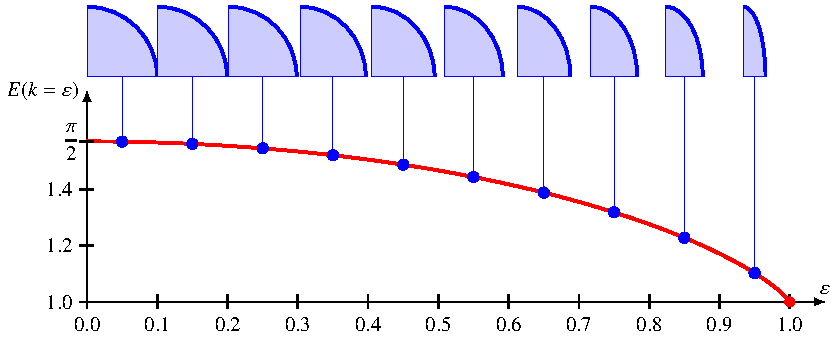
\includegraphics{chapters/110-elliptisch/images/ellipsenumfang.pdf}
\caption{Bogenlänge eines Viertels einer Ellipse mit Exzentrizität
$\varepsilon$.
\label{buch:elliptisch:fig:ellipsenumfang}}
\end{figure}
Wir zeigen, wie sich die Berechnung des Umfangs $U$ einer Ellipse
mit Halbachsen $a$ und $b$, $a\le b$, auf ein volltändiges elliptisches
Integral zurückführen lässt.
Der Fall $a>b$ kann behandelt werden, indem die $x$- und $y$-Koordinaten
vertauscht werden.

Die Parametrisierung
\[
t\mapsto \begin{pmatrix}a\cos t\\ b\sin t\end{pmatrix}
\]
einer Ellipse führt auf das Integral
\begin{align*}
U
&=
\int_0^{2\pi} \sqrt{a^2\sin^2t + b^2\cos^2 t}\,dt
\notag
\\
&=
4\int_0^{\frac{\pi}2}
\sqrt{a^2\sin^2t + b^2(1-\sin^2 t)}
\,dt
\notag
\\
&=
4b \int_0^{\frac{\pi}2} \sqrt{1-(b^2-a^2)/b^2\cdot \sin^2t}\,dt
\label{buch:elliptisch:eqn:umfangellipse}
\end{align*}
für den Umfang der Ellipse.
Bei einem Kreis ist $a=b$ und der zweite Term unter der Wurzel fällt weg,
der Umfang wird $4b\frac{\pi}2=2\pi b$.
Die Differenz $e^2=b^2-a^2$ ist die {\em lineare Exzentrizität} der Ellipse,
\index{lineare Exzentrizität}%
der Quotient $e/b$ wird die {\em numerische Exzentrizität} der Ellipse
genannt.
Insbesondere ist $k = \varepsilon$.

Das Integral~\eqref{buch:elliptisch:eqn:umfangellipse} erhält jetzt die
Form
\[
U
=
4b\int_0^{\frac{\pi}2} \sqrt{1-k^2\sin^2t}\,dt
\]
und ist damit als elliptisches Integral zweiter Art erkannt.
Für den Umfang der Ellipse finden wir damit die Formel
\[
U
=
4b E(k)
=
4b E(\varepsilon).
\]
Das vollständige elliptische Integral zweiter Art $E(\varepsilon)$
liefert also genau den Umfang der eines Viertels Ellipse mit
numerischer Exzentrizität $\varepsilon$ und kleiner Halbachse $1$.

\subsubsection{Komplementäre Integrale}
XXX Komplementäre Integrale \\

\subsubsection{Ableitung}
XXX Ableitung \\
XXX Stammfunktion \\

\subsection{Unvollständige elliptische Integrale}
XXX Vollständige und Unvollständige Integrale \\
XXX Additionstheoreme \\
XXX Parameterkonventionen \\

\subsection{Potenzreihe}
XXX Potenzreihen \\
XXX Als hypergeometrische Funktionen \\



\section{Jacobische elliptische Funktionen}

Für das elliptische Filter werden, wie es der Name bereits deutet, elliptische Funktionen gebraucht.
Wie die trigonometrischen Funktionen Zusammenhänge eines Kreises darlegen, beschreiben die elliptischen Funktionen Ellipsen.
Es ist daher naheliegend, dass der Kosinus des Tschebyscheff-Filters gegen ein elliptisches Pendant ausgetauscht werden könnte.
Der Begriff elliptische Funktion wird für sehr viele Funktionen gebraucht, daher ist es hier wichtig zu erwähnen, dass es ausschliesslich um die Jacobischen elliptischen Funktionen geht.

\subsection{Grundlegende Eigenschaften}

Die Jacobi elliptischen Funktionen werden ausführlich im Kapitel \ref{buch:elliptisch:section:jacobi} behandelt.
Im Wesentlichen erweitern die Jacobi elliptischen Funktionen die trigonometrische Funktionen für Ellipsen.
Zum Beispiel gibt es analog zum Sinus den elliptischen $\sn(z, k)$.
Im Gegensatz zum den trigonometrischen Funktionen haben die elliptischen Funktionen zwei Parameter.
Den \textit{elliptische Modul} $k$, der die Exzentrizität der Ellipse parametrisiert und das Winkelargument $z$.
Im Kreis ist der Radius für alle Winkel konstant, bei Ellipsen ändert sich das.
Dies hat zur Folge, dass bei einer Ellipse die Kreisbogenlänge nicht linear zum Winkel verläuft.
Darum kann hier nicht der gewohnte Winkel verwendet werden.
Das Winkelargument $z$ kann durch das elliptische Integral erster Art
\begin{equation}
    z
    =
    F(\phi, k)
    =
    \int_{0}^{\phi}
    \frac{
        d\theta
    }{
        \sqrt{
            1-k^2 \sin^2 \theta
        }
    }
\end{equation}
mit dem Winkel $\phi$ in Verbindung gebracht werden.

Dabei wird das vollständige und unvollständige elliptische integral unterschieden.
Beim vollständigen Integral
\begin{equation}
    K(k)
    =
    \int_{0}^{\pi / 2}
    \frac{
        d\theta
    }{
        \sqrt{
            1-k^2 \sin^2 \theta
        }
    }
\end{equation}
wird über ein viertel Ellipsenbogen integriert, also bis $\phi=\pi/2$ und liefert das Winkelargument für eine Vierteldrehung.
Die Zahl wird oft auch abgekürzt mit $K = K(k)$ und ist für das elliptische Filter sehr relevant.
Alle elliptischen Funktionen sind somit $4K$-periodisch.

Neben dem $\sn$ gibt es zwei weitere elliptische Basisfunktionen $\cn$ und $\dn$.
Dazu kommen noch weitere abgeleitete Funktionen, die durch Quotienten und Kehrwerte dieser Funktionen zustande kommen.
Insgesamt sind es die zwölf Funktionen
\begin{equation*}
    \sn \quad
    \ns \quad
    \scelliptic \quad
    \sd \quad
    \cn \quad
    \nc \quad
    \cs \quad
    \cd \quad
    \dn \quad
    \nd \quad
    \ds \quad
    \dc.
\end{equation*}

Die Jacobischen elliptischen Funktionen können mit der inversen Funktion des vollständigen elliptischen Integrals erster Art
\begin{equation}
    \phi = F^{-1}(z, k)
\end{equation}
definiert werden. Dabei ist zu beachten dass nur das $z$ Argument der Funktion invertiert wird, also
\begin{equation}
    z = F(\phi, k)
    \Leftrightarrow
    \phi = F^{-1}(z, k).
\end{equation}
Mithilfe von $F^{-1}$ kann zum Beispiel $sn^{-1}$ mit dem elliptischen Integral dargestellt werden:
\begin{equation}
    \sin(\phi)
    =
    \sin \left( F^{-1}(z, k) \right)
    =
    \sn(z, k)
    =
    w.
\end{equation}

% \begin{equation} %TODO remove unnecessary equations
%     \phi
%     =
%      F^{-1}(z, k)
%      =
%      \sin^{-1} \big( \sn (z, k ) \big)
%      =
%     \sin^{-1} ( w )
% \end{equation}

% \begin{equation}
%     F(\phi, k)
%     =
%     z
%     =
%     F( \sin^{-1} \big( \sn (z, k ) \big) , k)
%     =
%     F( \sin^{-1} ( w ), k)
% \end{equation}

% \begin{equation}
%     \sn^{-1}(w, k)
%     =
%     F(\phi, k),
%     \quad
%     \phi = \sin^{-1}(w)
% \end{equation}

\subsection{Die Funktion $\sn^{-1}$}

Beim Tschebyscheff-Filter konnten wir mit Betrachten des Arcuscosinus die Funktionalität erklären.
Für das Elliptische Filter machen wir die gleiche Betrachtung mit der $\sn^{-1}$-Funktion.
Der $\sn^{-1}$ ist durch das elliptische Integral
\begin{align}
    \sn^{-1}(w, k)
        & =
    \int_{0}^{\phi}
    \frac{
        d\theta
    }{
        \sqrt{
            1-k^2 \sin^2 \theta
        }
    },
    \quad
    \phi = \sin^{-1}(w)
    \\
        & =
    \int_{0}^{w}
    \frac{
        dt
    }{
        \sqrt{
            (1-t^2)(1-k^2 t^2)
        }
    }
\end{align}
beschrieben.
Dazu betrachten wir wieder den Integranden
\begin{equation}
    \frac{
        1
    }{
        \sqrt{
            (1-t^2)(1-k^2 t^2)
        }
    }.
\end{equation}
Beim $\cos^{-1}(x)$ haben wir gesehen, dass die analytische Fortsetzung bei $x < -1$ und $x > 1$ rechtwinklig in die komplexen Zahlen wandert.
Wenn man das Gleiche mit $\sn^{-1}(w, k)$ macht, erkennt man zwei interessante Stellen.
Die erste ist die gleiche wie beim $\cos^{-1}(x)$ nämlich bei $t = \pm 1$.
Der erste Term unter der Wurzel wird dann negativ, während der zweite noch positiv ist, da $k \leq 1$.
Ab diesem Punkt knickt die Funktion in die imaginäre Richtung ab.
Bei $t = 1/k$ ist auch der zweite Term negativ und die Funktion verläuft in die negative reelle Richtung.
Abbildung \ref{ellfilter:fig:sn} zeigt den Verlauf der Funktion in der komplexen Ebene.
\begin{figure}
    \centering
    \begin{tikzpicture}[>=stealth', auto, node distance=2cm, scale=1.2]

    \tikzstyle{zero} = [draw, circle, inner sep =0, minimum height=0.15cm]

    \tikzset{pole/.style={cross out, draw=black, minimum size=(0.15cm-\pgflinewidth), inner sep=0pt, outer sep=0pt}}

    \begin{scope}[xscale=0.9, yscale=1.8]

        \draw[gray, ->] (0,-1.5) -- (0,1.5) node[anchor=south]{$\mathrm{Im}~z$};
        \draw[gray, ->] (-5,0) -- (5,0) node[anchor=west]{$\mathrm{Re}~z$};

        \begin{scope}

            \clip(-4.5,-1.25) rectangle (4.5,1.25);

            \fill[yellow!30] (0,0) rectangle (1, 0.5);

            \begin{scope}[xshift=-1cm]

                \foreach \i in {-2,...,2} {
                    \foreach \j in {-2,...,1} {
                        \begin{scope}[xshift=\i*4cm, yshift=\j*1cm]
                            \draw[<-, blue!50] (0, 0) -- (0,0.5);
                            \draw[<-, cyan!50] (1, 0) -- (0,0);
                            \draw[<-, darkgreen!50] (2, 0) -- (1,0);
                            \draw[<-, orange!50] (2,0.5) -- (2, 0);
                            \draw[<-, red!50] (1, 0.5) -- (2,0.5);
                            \draw[<-, purple!50] (0, 0.5) -- (1,0.5);
                            \draw[<-, blue!50] (0,1) -- (0,0.5);
                            \draw[<-, orange!50] (2,0.5) -- (2, 1);
                            \draw[<-, red!50] (3, 0.5) -- (2,0.5);
                            \draw[<-, purple!50] (4, 0.5) -- (3,0.5);
                            \draw[<-, darkgreen!50] (2, 0) -- (3,0);
                            \draw[<-, cyan!50] (3, 0) -- (4,0);
                        \end{scope}
                    }
                }

                % \pause
                \draw[ultra thick, <-, darkgreen] (2, 0) -- (1,0);
                % \pause
                \draw[ultra thick, <-, orange] (2,0.5) -- (2, 0);
                % \pause
                \draw[ultra thick, <-, red] (1, 0.5) -- (2,0.5);
                % \pause
                \draw[ultra thick, <-, blue] (0, 0) -- (0,0.5);
                \draw[ultra thick, <-, purple] (0, 0.5) -- (1,0.5);
                \draw[ultra thick, <-, cyan] (1, 0) -- (0,0);
                % \pause


                \foreach \i in {-2,...,2} {
                    \foreach \j in {-2,...,1} {
                        \begin{scope}[xshift=\i*4cm, yshift=\j*1cm]
                            \node[zero] at ( 1, 0) {};
                            \node[zero] at ( 3, 0) {};
                            \node[pole] at ( 1,0.5) {};
                            \node[pole] at ( 3,0.5) {};
                        \end{scope}
                    }
                }

            \end{scope}

        \end{scope}

        \draw[gray] ( 1,0) +(0,0.1) -- +(0, -0.1) node[inner sep=0, anchor=north] {\small $K$};
        \draw[gray]  (0, 0.5) +(0.1, 0) -- +(-0.1, 0) node[inner sep=0, anchor=east]{\small $jK^\prime$};

    \end{scope}

    \node[zero] at (4,3) (n) {};
    \node[anchor=west] at (n.east) {Zero};
    \node[pole, below=0.25cm of n] (n) {};
    \node[anchor=west] at (n.east) {Pole};

    \begin{scope}[yshift=-4cm, xscale=0.75]

        \draw[gray, ->] (-6,0) -- (6,0) node[anchor=west]{$w$};

        \draw[ultra thick, ->, purple] (-5, 0) -- (-3, 0);
        \draw[ultra thick, ->, blue]      (-3, 0) -- (-2, 0);
        \draw[ultra thick, ->, cyan]       (-2, 0) -- (0, 0);
        \draw[ultra thick, ->, darkgreen]    (0, 0) -- (2, 0);
        \draw[ultra thick, ->, orange] (2, 0) -- (3, 0);
        \draw[ultra thick, ->, red] (3, 0) -- (5, 0);

        \node[anchor=south] at (-5,0) {$-\infty$};
        \node[anchor=south] at (-3,0) {$-1/k$};
        \node[anchor=south] at (-2,0) {$-1$};
        \node[anchor=south] at (0,0) {$0$};
        \node[anchor=south] at (2,0) {$1$};
        \node[anchor=south] at (3,0) {$1/k$};
        \node[anchor=south] at (5,0) {$\infty$};

    \end{scope}


\end{tikzpicture}
    \caption{
        $z$-Ebene der Funktion $z = \sn^{-1}(w, k)$.
        Die Funktion ist in der realen Achse $4K$-periodisch und in der imaginären Achse $2jK^\prime$-periodisch.
    }
    \label{ellfilter:fig:sn}
\end{figure}
In der reellen Richtung ist sie $4K(k)$-periodisch und in der imaginären Richtung $4K^\prime(k)$-periodisch, wobei $K^\prime$ das komplementäre vollständige Elliptische Integral ist:
\begin{equation}
    K^\prime(k)
    =
    \int_{0}^{\pi / 2}
    \frac{
        d\theta
    }{
        \sqrt{
            1-{k^\prime}^2 \sin^2 \theta
        }
    },
    \quad
    k^\prime = \sqrt{1-k^2}.
\end{equation}

%
% lemniskate.tex
%
% (c) 2021 Prof Dr Andreas Müller, OST Ostschweizer Fachhochschule
%
\section{Lemniskatischer Sinus
\label{buch:elliptisch:section:lemniskate}}
\rhead{Lemniskatischer Sinus}
Historisch war der {\em lemniskatische Sinus} die erste ellptische
Funktion, die Gauss bereits als 19-jähriger untersucht, aber nicht 
veröffentlich hat.
In diesem Abschnitt soll die Verbindung zu den Jacobischen
elliptischen Funktionen hergestellt werden.

\subsection{Lemniskate
\label{buch:gemotrie:subsection:lemniskate}}
\begin{figure}
\centering
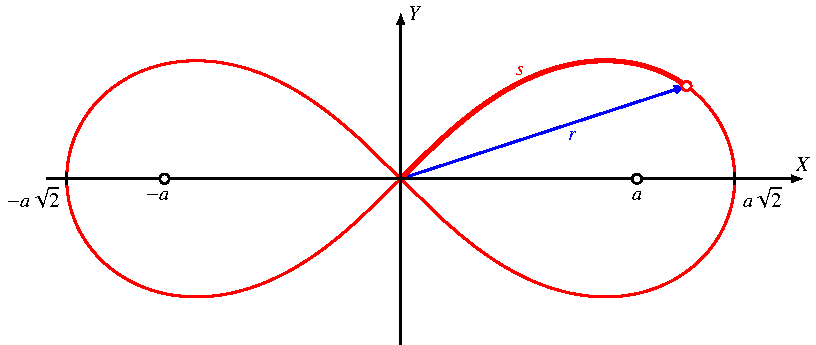
\includegraphics{chapters/110-elliptisch/images/lemniskate.pdf}
\caption{Bogenlänge und Radius der Lemniskate von Bernoulli.
\label{buch:elliptisch:fig:lemniskate}}
\end{figure}
Die Lemniskate von Bernoulli ist die Kurve vierten Grades mit der Gleichung
\begin{equation}
(X^2+Y^2)^2 = 2a^2(X^2-Y^2).
\label{buch:elliptisch:eqn:lemniskate}
\end{equation}
Sie ist in Abbildung~\ref{buch:elliptisch:fig:lemniskate}
dargestellt.
Die beiden Scheitel der Lemniskate befinden sich bei $X_s=\pm a\sqrt{2}$.
Dividiert man die Gleichung der Lemniskate durch $X_s^2=4a^4$ entsteht 
\begin{equation}
\biggl(
\biggl(\frac{X}{a\sqrt{2}}\biggr)^2
+
\biggl(\frac{Y}{a\sqrt{2}}\biggr)^2
\biggr)^2
=
2\frac{a^2}{2a^2}\biggl(
\biggl(\frac{X}{a\sqrt{2}}\biggr)^2
-
\biggl(\frac{Y}{a\sqrt{2}}\biggr)^2
\biggr).
\qquad
\Leftrightarrow
\qquad
(x^2+y^2)^2 = x^2-y^2,
\label{buch:elliptisch:eqn:lemniskatenormiert}
\end{equation}
wobei wir $x=X/a\sqrt{2}$ und $y=Y/a\sqrt{2}$ gesetzt haben.
In dieser Normierung liegen die Scheitel bei $\pm 1$.
Dies ist die Skalierung, die für die Definition des lemniskatischen
Sinus und Kosinus verwendet werden soll.

In Polarkoordinaten $x=r\cos\varphi$ und $y=r\sin\varphi$
gilt nach Einsetzen in \eqref{buch:elliptisch:eqn:lemniskatenormiert}
\begin{equation}
r^4
=
r^2(\cos^2\varphi-\sin^2\varphi)
=
r^2\cos2\varphi
\qquad\Rightarrow\qquad
r^2 = \cos 2\varphi
\label{buch:elliptisch:eqn:lemniskatepolar}
\end{equation}
als Darstellung der Lemniskate in Polardarstellung.
Sie gilt für Winkel $\varphi\in[-\frac{\pi}4,\frac{\pi}4]$ für das
rechte Blatt und $\varphi\in[\frac{3\pi}4,\frac{5\pi}4]$ für das linke
Blatt der Lemniskate.

\subsection{Bogenlänge}
Die Funktionen
\begin{equation}
x(r) = \frac{r}{\sqrt{2}}\sqrt{1+r^2},
\quad
y(r) = \frac{r}{\sqrt{2}}\sqrt{1-r^2}
\label{buch:geometrie:eqn:lemniskateparam}
\end{equation}
erfüllen
\begin{align*}
x(r)^2-y(r)^2
&=
\frac{r^2(1+r^2)}{2}-\frac{r^2(1-r^2)}{2}
\\
&
=
r^4
=
(x(r)^2 + y(r)^2)^2,
\end{align*}
sie stellen also eine Parametrisierung der Lemniskate dar.

Mit Hilfe der Parametrisierung~\eqref{buch:geometrie:eqn:lemniskateparam}
kann man die Länge $s$ des in Abbildung~\ref{buch:elliptisch:fig:lemniskate}
dargestellten Bogens der Lemniskate berechnen.
Dazu benötigt man die Ableitungen nach $r$, die man mit der Produkt- und
Kettenregel berechnen kann:
\begin{align*}
\dot{x}(r)
&=
\frac{\sqrt{1+r^2}}{\sqrt{2}}
+
\frac{r^2}{\sqrt{2}\sqrt{1+r^2}}
&&\Rightarrow&
\dot{x}(r)^2
&=
\frac{1+r^2}{2} +r^2 + \frac{r^4}{2(1+r^2)}
\\
\dot{y}(r)
&=
\frac{\sqrt{1-r^2}}{\sqrt{2}}
-
\frac{r^2}{\sqrt{2}\sqrt{1-r^2}}
&&\Rightarrow&
\dot{y}(r)^2
&=
\frac{1-r^2}{2} -r^2 + \frac{r^4}{2(1-r^2)}
\end{align*}
Die Summe der Quadrate ist
\begin{align*}
\dot{x}(r)^2 + \dot{y}(r)^2
&=
1 + r^4\frac{1-r^2+1+r^2}{2(1+r^2)(1-r^2)}
=
1+r^4\frac{2}{2(1-r^4)}
=
\frac{1-r^4+r^4}{1-r^4}
=
\frac1{1-r^4}.
\end{align*}
Durch Einsetzen in das Integral für die Bogenlänge bekommt man
\begin{equation}
s(r)
=
\int_0^r
\frac{1}{\sqrt{1-t^4}}\,dt.
\label{buch:elliptisch:eqn:lemniskatebogenlaenge}
\end{equation}

%
% Als elliptisches Integral
%
\subsection{Darstellung als elliptisches Integral}
Das unvollständige elliptische Integral erster Art mit Parameter
$k^2=-1$ oder $k=i$ ist
\[
K(r,i)
=
\int_0^x \frac{dt}{\sqrt{(1-t^2)(1-i^2 t^2)}}
=
\int_0^x \frac{dt}{\sqrt{(1-t^2)(1-(-1)t^2)}}
=
\int_0^x \frac{dt}{\sqrt{1-t^4}}
=
s(r).
\]
Der lemniskatische Sinus ist also eine Umkehrfunktion des
elliptischen Integrals erster Art für den speziellen Wert $i$ des
Parameters $k$.

Die Länge des rechten Blattes der Lemniskate wird mit $\varpi$ bezeichnet
und hat den numerischen Wert
\[
\varpi
=
2\int_0^1\sqrt{\frac{1}{1-t^4}}\,dt
=
2.6220575542.
\]
$\varpi$ ist auch als die {\em lemniskatische Konstante} bekannt.
\index{lemniskatische Konstante}%
Der Lemniskatenbogen zwischen dem Nullpunkt und $(1,0)$ hat die Länge
$\varpi/2$.

%
%  Bogenlängenparametrisierung
%
\subsection{Bogenlängenparametrisierung}
Die Lemniskate mit der Gleichung
\[
(X^2+X^2)^2=2(X^2-X^2)
\]
(der Fall $a=1$ in \eqref{buch:elliptisch:eqn:lemniskate})
kann mit Jacobischen elliptischen Funktionen
parametrisiert werden.
Dazu schreibt man
\[
\left.
\begin{aligned}
X(t)
&=
\sqrt{2}\operatorname{cn}(t,k) \operatorname{dn}(t,k)
\\
Y(t)
&=
\phantom{\sqrt{2}}
\operatorname{cn}(t,k) \operatorname{sn}(t,k)
\end{aligned}
\quad\right\}
\qquad\text{mit $k=\displaystyle\frac{1}{\sqrt{2}}$}
\]
und berechnet die beiden Seiten der definierenden Gleichung der
Lemniskate.
Zunächst ist
\begin{align*}
X(t)^2
&=
2\operatorname{cn}(t,k)^2
\operatorname{dn}(t,k)^2
\\
Y(t)^2
&=
\operatorname{cn}(t,k)^2
\operatorname{sn}(t,k)^2
\\
X(t)^2+Y(t)^2
&=
2\operatorname{cn}(t,k)^2
\bigl(
\underbrace{
\operatorname{dn}(t,k)^2
+{\textstyle\frac12}
\operatorname{sn}(t,k)^2
}_{\displaystyle =1}
\bigr)
%\\
%&
=
2\operatorname{cn}(t,k)^2
\\
X(t)^2-Y(t)^2
&=
\operatorname{cn}(t,k)^2
\bigl(
2\operatorname{dn}(t,k)^2 - \operatorname{sn}(t,k)^2
\bigr)
\\
&=
\operatorname{cn}(t,k)^2
\bigl(
2\bigl({\textstyle\frac12}+{\textstyle\frac12}\operatorname{cn}(t,k)^2\bigr)
-
\bigl(1-\operatorname{cn}(t,k)^2\bigr)
\bigr)
\\
&=
2\operatorname{cn}(t,k)^4
\\
\Rightarrow\qquad
(X(t)^2+Y(t)^2)^2
&=
4\operatorname{cn}(t,k)^4
=
2(X(t)^2-Y(t)^2).
\end{align*}
Wir zeigen jetzt, dass dies tatsächlich eine Bogenlängenparametrisierung
der Lemniskate ist.
Dazu berechnen wir die Ableitungen
\begin{align*}
\dot{X}(t)
&=
\sqrt{2}\operatorname{cn}'(t,k)\operatorname{dn}(t,k)
+
\sqrt{2}\operatorname{cn}(t,k)\operatorname{dn}'(t,k)
\\
&=
-\sqrt{2}\operatorname{sn}(t,k)\operatorname{dn}(t,k)^2
-\frac12\sqrt{2}\operatorname{sn}(t,k)\operatorname{cn}(t,k)^2
\\
&=
-\sqrt{2}\operatorname{sn}(t,k)\bigl(
1-{\textstyle\frac12}\operatorname{sn}(t,k)^2
+{\textstyle\frac12}-{\textstyle\frac12}\operatorname{sn}(u,t)^2
\bigr)
\\
&=
\sqrt{2}\operatorname{sn}(t,k)
\bigl(
{\textstyle \frac32}-\operatorname{sn}(t,k)^2
\bigr)
\\
\dot{X}(t)^2
&=
2\operatorname{sn}(t,k)^2
\bigl(
{\textstyle \frac32}-\operatorname{sn}(t,k)^2
\bigr)^2
\\
&=
{\textstyle\frac{9}{2}}\operatorname{sn}(t,k)^2
-
6\operatorname{sn}(t,k)^4
+2\operatorname{sn}(t,k)^6
\\
\dot{Y}(t)
&=
\operatorname{cn}'(t,k)\operatorname{sn}(t,k)
+
\operatorname{cn}(t,k)\operatorname{sn}'(t,k)
\\
&=
-\operatorname{sn}(t,k)^2
\operatorname{dn}(t,k)
+\operatorname{cn}(t,k)^2
\operatorname{dn}(t,k)
\\
&=
\operatorname{dn}(t,k)\bigl(1-2\operatorname{sn}(t,k)^2\bigr)
\\
\dot{Y}(t)^2
&=
\bigl(1-{\textstyle\frac12}\operatorname{sn}(t,k)^2\bigr)
\bigl(1-2\operatorname|{sn}(t,k)^2\bigr)^2
\\
&=
1-{\textstyle\frac{9}{2}}\operatorname{sn}(t,k)^2
+6\operatorname{sn}(t,k)^4
-2\operatorname{sn}(t,k)^6
\\
\dot{X}(t)^2 + \dot{Y}(t)^2
&=
1.
\end{align*}
Dies bedeutet, dass die Bogenlänge zwischen den Parameterwerten $0$ und $s$
\[
\int_0^s
\sqrt{\dot{X}(t)^2 + \dot{Y}(t)^2}
\,dt
=
\int_0^s\,dt
=
s,
\]
der Parameter $t$ ist also ein Bogenlängenparameter.

Die mit dem Faktor $1/\sqrt{2}$ skalierte Standard-Lemniskate mit der
Gleichung
\[
(x^2+y^2)^2 = x^2-y^2
\]
hat daher eine Bogenlängenparametrisierung mit
\begin{equation}
\begin{aligned}
x(t)
&=
\phantom{\frac{1}{\sqrt{2}}}
\operatorname{cn}(\sqrt{2}t,k)\operatorname{dn}(\sqrt{2}t,k)
\\
y(t)
&=
\frac{1}{\sqrt{2}}\operatorname{cn}(\sqrt{2}t,k)\operatorname{sn}(\sqrt{2}t,k)
\end{aligned}
\label{buch:elliptisch:lemniskate:bogenlaenge}
\end{equation}

\subsection{Der lemniskatische Sinus und Kosinus}
Der Sinus Berechnet die Gegenkathete zu einer gegebenen Bogenlänge des
Kreises, er ist die Umkehrfunktion der Funktion, die der Gegenkathete
die Bogenlänge zuordnet.

Daher ist es naheliegend, die Umkehrfunktion von $s(r)$ in 
\eqref{buch:elliptisch:eqn:lemniskatebogenlaenge}
den {\em lemniskatischen Sinus} zu nennen mit der Bezeichnung
$r=\operatorname{sl} s$.

Der Kosinus ist der Sinus des komplementären Winkels.
Auch für die lemniskatische Bogenlänge $s(r)$ lässt sich eine
komplementäre Bogenlänge definieren, nämlich die Bogenlänge zwischen
dem Punkt $(x(r), y(r))$ und $(1,0)$.

Da die Parametrisierung~\eqref{buch:elliptisch:lemniskate:bogenlaenge}
eine Bogenlängenparametrisierung ist, darf man $t=s$ schreiben.
Dann kann man aber auch $r(s)$ daraus berechnen,
es ist
\[
r(s)^2
=
x(s)^2 + y(s)^2
=
\operatorname{cn}(s\sqrt{2},k)^2
\qquad\Rightarrow\qquad
r(s)
=
\operatorname{cn}(s\sqrt{2},k)
\]

\begin{figure}
\centering
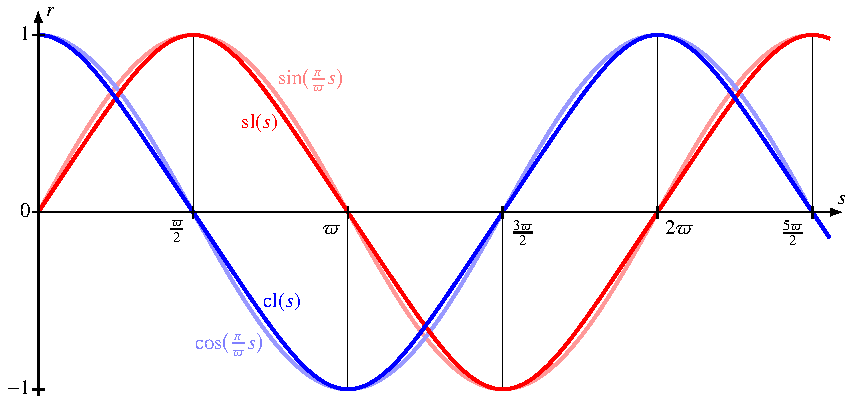
\includegraphics{chapters/110-elliptisch/images/slcl.pdf}
\caption{
Lemniskatischer Sinus und Kosinus sowie Sinus und Kosinus
mit derart skaliertem Argument, dass die Funktionen die gleichen Nullstellen
haben.
\label{buch:elliptisch:figure:slcl}}
\end{figure}


%\section*{Übungsaufgaben}
%\rhead{Übungsaufgaben}
%\aufgabetoplevel{chapters/020-exponential/uebungsaufgaben}
%\begin{uebungsaufgaben}
%\uebungsaufgabe{0}
%\uebungsaufgabe{1}
%\end{uebungsaufgaben}


%%
% chapter.tex -- Beschreibung des Inhaltes
%
% (c) 2021 Prof Dr Andreas Müller, Hochschule Rapperswil
%
% !TeX spellcheck = de_CH
\chapter{Elliptische Funktionen
\label{buch:chapter:geometrie}}
\lhead{Elliptische Funktionen}
\rhead{}

Der Versuch, die Länge eines Ellipsenbogens zu berechnen, hat
in Abschnitt~\ref{buch:geometrie:subsection:hyperbeln-und-ellipsen}
zu Integralen geführt, die nicht in geschlossener Form ausgewertet
werden können.
Neben den dort gefundenen Integralen sind noch weitere, ähnlich
aufgebaute Integrale in dieser Familie zu finden.

%
% ellintegral.tex
%
% (c) 2021 Prof Dr Andreas Müller, OST Ostschweizer Fachhochschule
%
\section{Elliptische Integrale
\label{buch:elliptisch:section:integral}}
\rhead{Elliptisches Integral}
Bei der Berechnung des Ellipsenbogens in 
Abschnitt~\ref{buch:geometrie:subsection:hyperbeln-und-ellipsen}
sind wir auf ein Integral gestossen, welches sich nicht in geschlossener
Form ausdrücken liess.
Um solche Integrale in den Griff zu bekommen, ist es nötig, sie als
neue spezielle Funktionen zu definieren.

\subsection{Definition
\label{buch:elliptisch:subsection:definition}}
Ein {\em elliptisches Integral} ist ein Integral der Form
\index{elliptishes Integral}%
\index{Integral, elliptisch}%
\begin{equation}
\int R\left( x, \sqrt{p(x)}\right)\,dx
\label{buch:elliptisch:def:allgemein}
\end{equation}
wobei $R(x,y)$ eine rationale Funktion von zwei Variablen ist und
$p(x)$ ein Polynom dritten oder vierten Grades.
Hätte $p(x)$ ein mehrfache Nullstelle $x_0$, müsste es durch $(x-x_0)^2$
teilbar sein, man könnte also einen Faktor $(x-x_0)$ aus der
Wurzel im Integraneden von \eqref{buch:elliptisch:def:allgemein}
ausklammern und damit das Integral in eine Form bringen, wo $p(x)$
höchstens zweiten Grades ist.
Solche Integrale lassen sich meistens mit trigonometrischen Substitutionen
berechnen.
Wir verlangen daher, dass $p(x)$ keine mehrfachen Nullstellen hat.

Man kann zeigen, dass sich elliptische Integrale in Summen von
elementaren Funktionen und speziellen elliptischen Integralen 
der folgenden Form überführen lassen
\cite[Abschnitt 164, p.~506]{buch:smirnov32}.

\begin{definition}
\label{buch:elliptisch:def:integrale123}
Die elliptischen Integrale erster, zweiter und dritter Art sind die
Integrale
\[
\begin{aligned}
\text{1.~Art:}&&&
\int \frac{dx}{\sqrt{(1-x^2)(1-k^2x^2)}}
\\
\text{2.~Art:}&&&
\int \sqrt{\frac{1-k^2x^2}{1-x^2}}\,dx
\\
\text{3.~Art:}&&&
\int \frac{dx}{(1-nx^2)\sqrt{(1-x^2)(1-k^2x^2)}}
\end{aligned}
\]
mit $0<k<1$.
Es ist auch üblich, den Parameter $m=k^2$ zu verwenden.
\end{definition}

Wie gesagt lassen sich für diese unbestimmten Integrale keine 
geschlossenen Formen finden.
Es bleibt uns daher nichts anderes übrig, als die Integralgrenzen
festzulegen und damit eine Stammfunktion auszuwählen.

%
% Elliptisches Integral
%
\subsection{Vollständige elliptische Integrale
\label{buch:elliptisch:subsection:vollstaendig}}
In diesem Abschnitt legen wir beide Integrationsgrenzen fest und
untersuchen die entstehenenden Funktionen von den Parametern
$k$ und $n$.

\subsubsection{Definition der vollständigen elliptischen Integrale}
Da der Nenner in allen drei elliptischen Integralen eine Nullstelle
bei $\pm1$ hat, kann das Integral nur von $0$ bis $1$ erstreckt werden.

\begin{definition}
\label{buch:elliptisch:def:vollstintegrale123}
Die vollständigen elliptischen Integrale erster, zweiter und dritter
Art sind
\[
\begin{aligned}
\text{1.~Art:}&&
K(k)&=\int_0^1 \frac{dt}{\sqrt{(1-t^2)(1-k^2t^2)}} \\
\text{2.~Art:}&&
E(k)&=\int_0^1 \sqrt{\frac{1-k^2t^2}{1-t^2}}\,dt \\
\text{3.~Art:}&&
\Pi(n, k)&=\int_0^1\frac{dt}{(1-nt^2)\sqrt{(1-t^2)(1-k^2t^2)}} 
\end{aligned}
\]
mit $0<k<1$.
\end{definition}

Die Funktionen hängen stetig von $k$ ab.
Die Nullstellen des Faktors $1-k^2x^2$ liegen ausserhalb des
Integrationsintervalls und spielen daher keine Rolle.
Die Werte von $K(k)$ und $E(k)$ für $k=0$ können direkt berechnet
werden:
\begin{align*}
K(0)
=
E(0)
&=
\int_0^1 \frac{dt}{\sqrt{1-t^2}}=\frac{\pi}2.
\end{align*}
Das Integral $\Pi(n,0)$ ist etwas komplizierter.

Für $k\to 1$ ist $E(k)=1$, die Integrale $K(1)$ und $\Pi(n,1)$
sind dagegen divergent.

\subsubsection{Jacobi- und Legendre-Normalform}
Die Integrationsvariable $t$ der vollständigen elliptischen Integrale
kann durch die Substitution $t=\sin\varphi$ durch die Variable
$\varphi$ und das Integral über das Intervall $[0,1]$ durch ein
Integral über das Intervall $[0,\frac{\pi}2]$ ersetzt werden.
Mit
\[
\frac{dt}{d\varphi} = \cos\varphi = \sqrt{1-\sin^2\varphi}
\]
können die Funktionen $K(k)$, $E(k)$ und $\Pi(n,k)$ auch als
\begin{align*}
K(k)
&=
\int_0^{\frac{\pi}2}
\frac{
\sqrt{1-\sin^2\varphi}\,d\varphi
}{
\sqrt{(1-\sin^2\varphi)(1-k^2\sin^2\varphi)}
}
=
\int_0^{\frac{\pi}2}
\frac{d\varphi}{\sqrt{1-k^2\sin^2\varphi}}
\\
E(k)
&=
\int_0^{\frac{\pi}2}
\sqrt{\frac{1-k^2\sin^2\varphi}{1-\sin^2\varphi}}\sqrt{1-\sin^2\varphi}\,d\varphi
=
\int_0^{\frac{\pi}2}
\sqrt{1-k^2\sin^2\varphi}\,d\varphi
\\
\Pi(n,k)
&=
\int_0^{\frac{\pi}2}
\frac{
\sqrt{1-\sin^2\varphi}\,d\varphi
}{
(1-n\sin^2\varphi)\sqrt{(1-\sin^2\varphi)(1-k^2\sin^2\varphi)}
}
=
\int_0^{\frac{\pi}2}
\frac{
d\varphi
}{
(1-n\sin^2\varphi)\sqrt{1-k^2\sin^2\varphi}
}
\end{align*}
Diese Form wird auch die {\em Legendre-Normalform} der vollständigen 
\index{Legendre-Normalform}%
elliptischen Integrale genannt, während die Form von
Definition~\ref{buch:elliptisch:def:vollstintegrale123}
die {\em Jacobi-Normalform} heisst.
\index{Jacobi-Normalform}%

\subsubsection{Umfang einer Ellipse}
\begin{figure}
\centering
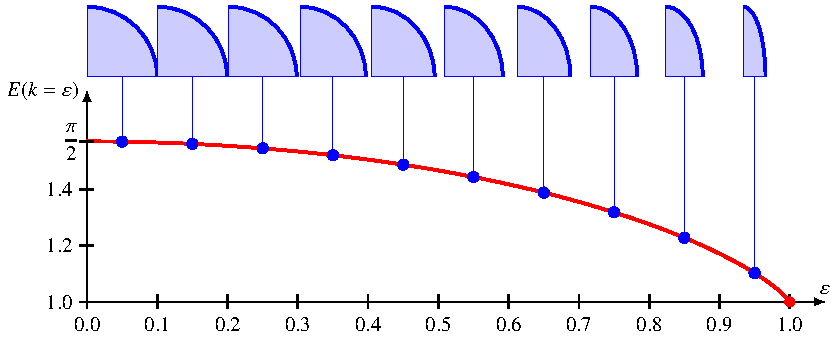
\includegraphics{chapters/110-elliptisch/images/ellipsenumfang.pdf}
\caption{Bogenlänge eines Viertels einer Ellipse mit Exzentrizität
$\varepsilon$.
\label{buch:elliptisch:fig:ellipsenumfang}}
\end{figure}
Wir zeigen, wie sich die Berechnung des Umfangs $U$ einer Ellipse
mit Halbachsen $a$ und $b$, $a\le b$, auf ein volltändiges elliptisches
Integral zurückführen lässt.
Der Fall $a>b$ kann behandelt werden, indem die $x$- und $y$-Koordinaten
vertauscht werden.

Die Parametrisierung
\[
t\mapsto \begin{pmatrix}a\cos t\\ b\sin t\end{pmatrix}
\]
einer Ellipse führt auf das Integral
\begin{align*}
U
&=
\int_0^{2\pi} \sqrt{a^2\sin^2t + b^2\cos^2 t}\,dt
\notag
\\
&=
4\int_0^{\frac{\pi}2}
\sqrt{a^2\sin^2t + b^2(1-\sin^2 t)}
\,dt
\notag
\\
&=
4b \int_0^{\frac{\pi}2} \sqrt{1-(b^2-a^2)/b^2\cdot \sin^2t}\,dt
\label{buch:elliptisch:eqn:umfangellipse}
\end{align*}
für den Umfang der Ellipse.
Bei einem Kreis ist $a=b$ und der zweite Term unter der Wurzel fällt weg,
der Umfang wird $4b\frac{\pi}2=2\pi b$.
Die Differenz $e^2=b^2-a^2$ ist die {\em lineare Exzentrizität} der Ellipse,
\index{lineare Exzentrizität}%
der Quotient $e/b$ wird die {\em numerische Exzentrizität} der Ellipse
genannt.
Insbesondere ist $k = \varepsilon$.

Das Integral~\eqref{buch:elliptisch:eqn:umfangellipse} erhält jetzt die
Form
\[
U
=
4b\int_0^{\frac{\pi}2} \sqrt{1-k^2\sin^2t}\,dt
\]
und ist damit als elliptisches Integral zweiter Art erkannt.
Für den Umfang der Ellipse finden wir damit die Formel
\[
U
=
4b E(k)
=
4b E(\varepsilon).
\]
Das vollständige elliptische Integral zweiter Art $E(\varepsilon)$
liefert also genau den Umfang der eines Viertels Ellipse mit
numerischer Exzentrizität $\varepsilon$ und kleiner Halbachse $1$.

\subsubsection{Komplementäre Integrale}
XXX Komplementäre Integrale \\

\subsubsection{Ableitung}
XXX Ableitung \\
XXX Stammfunktion \\

\subsection{Unvollständige elliptische Integrale}
XXX Vollständige und Unvollständige Integrale \\
XXX Additionstheoreme \\
XXX Parameterkonventionen \\

\subsection{Potenzreihe}
XXX Potenzreihen \\
XXX Als hypergeometrische Funktionen \\



\section{Jacobische elliptische Funktionen}

Für das elliptische Filter werden, wie es der Name bereits deutet, elliptische Funktionen gebraucht.
Wie die trigonometrischen Funktionen Zusammenhänge eines Kreises darlegen, beschreiben die elliptischen Funktionen Ellipsen.
Es ist daher naheliegend, dass der Kosinus des Tschebyscheff-Filters gegen ein elliptisches Pendant ausgetauscht werden könnte.
Der Begriff elliptische Funktion wird für sehr viele Funktionen gebraucht, daher ist es hier wichtig zu erwähnen, dass es ausschliesslich um die Jacobischen elliptischen Funktionen geht.

\subsection{Grundlegende Eigenschaften}

Die Jacobi elliptischen Funktionen werden ausführlich im Kapitel \ref{buch:elliptisch:section:jacobi} behandelt.
Im Wesentlichen erweitern die Jacobi elliptischen Funktionen die trigonometrische Funktionen für Ellipsen.
Zum Beispiel gibt es analog zum Sinus den elliptischen $\sn(z, k)$.
Im Gegensatz zum den trigonometrischen Funktionen haben die elliptischen Funktionen zwei Parameter.
Den \textit{elliptische Modul} $k$, der die Exzentrizität der Ellipse parametrisiert und das Winkelargument $z$.
Im Kreis ist der Radius für alle Winkel konstant, bei Ellipsen ändert sich das.
Dies hat zur Folge, dass bei einer Ellipse die Kreisbogenlänge nicht linear zum Winkel verläuft.
Darum kann hier nicht der gewohnte Winkel verwendet werden.
Das Winkelargument $z$ kann durch das elliptische Integral erster Art
\begin{equation}
    z
    =
    F(\phi, k)
    =
    \int_{0}^{\phi}
    \frac{
        d\theta
    }{
        \sqrt{
            1-k^2 \sin^2 \theta
        }
    }
\end{equation}
mit dem Winkel $\phi$ in Verbindung gebracht werden.

Dabei wird das vollständige und unvollständige elliptische integral unterschieden.
Beim vollständigen Integral
\begin{equation}
    K(k)
    =
    \int_{0}^{\pi / 2}
    \frac{
        d\theta
    }{
        \sqrt{
            1-k^2 \sin^2 \theta
        }
    }
\end{equation}
wird über ein viertel Ellipsenbogen integriert, also bis $\phi=\pi/2$ und liefert das Winkelargument für eine Vierteldrehung.
Die Zahl wird oft auch abgekürzt mit $K = K(k)$ und ist für das elliptische Filter sehr relevant.
Alle elliptischen Funktionen sind somit $4K$-periodisch.

Neben dem $\sn$ gibt es zwei weitere elliptische Basisfunktionen $\cn$ und $\dn$.
Dazu kommen noch weitere abgeleitete Funktionen, die durch Quotienten und Kehrwerte dieser Funktionen zustande kommen.
Insgesamt sind es die zwölf Funktionen
\begin{equation*}
    \sn \quad
    \ns \quad
    \scelliptic \quad
    \sd \quad
    \cn \quad
    \nc \quad
    \cs \quad
    \cd \quad
    \dn \quad
    \nd \quad
    \ds \quad
    \dc.
\end{equation*}

Die Jacobischen elliptischen Funktionen können mit der inversen Funktion des vollständigen elliptischen Integrals erster Art
\begin{equation}
    \phi = F^{-1}(z, k)
\end{equation}
definiert werden. Dabei ist zu beachten dass nur das $z$ Argument der Funktion invertiert wird, also
\begin{equation}
    z = F(\phi, k)
    \Leftrightarrow
    \phi = F^{-1}(z, k).
\end{equation}
Mithilfe von $F^{-1}$ kann zum Beispiel $sn^{-1}$ mit dem elliptischen Integral dargestellt werden:
\begin{equation}
    \sin(\phi)
    =
    \sin \left( F^{-1}(z, k) \right)
    =
    \sn(z, k)
    =
    w.
\end{equation}

% \begin{equation} %TODO remove unnecessary equations
%     \phi
%     =
%      F^{-1}(z, k)
%      =
%      \sin^{-1} \big( \sn (z, k ) \big)
%      =
%     \sin^{-1} ( w )
% \end{equation}

% \begin{equation}
%     F(\phi, k)
%     =
%     z
%     =
%     F( \sin^{-1} \big( \sn (z, k ) \big) , k)
%     =
%     F( \sin^{-1} ( w ), k)
% \end{equation}

% \begin{equation}
%     \sn^{-1}(w, k)
%     =
%     F(\phi, k),
%     \quad
%     \phi = \sin^{-1}(w)
% \end{equation}

\subsection{Die Funktion $\sn^{-1}$}

Beim Tschebyscheff-Filter konnten wir mit Betrachten des Arcuscosinus die Funktionalität erklären.
Für das Elliptische Filter machen wir die gleiche Betrachtung mit der $\sn^{-1}$-Funktion.
Der $\sn^{-1}$ ist durch das elliptische Integral
\begin{align}
    \sn^{-1}(w, k)
        & =
    \int_{0}^{\phi}
    \frac{
        d\theta
    }{
        \sqrt{
            1-k^2 \sin^2 \theta
        }
    },
    \quad
    \phi = \sin^{-1}(w)
    \\
        & =
    \int_{0}^{w}
    \frac{
        dt
    }{
        \sqrt{
            (1-t^2)(1-k^2 t^2)
        }
    }
\end{align}
beschrieben.
Dazu betrachten wir wieder den Integranden
\begin{equation}
    \frac{
        1
    }{
        \sqrt{
            (1-t^2)(1-k^2 t^2)
        }
    }.
\end{equation}
Beim $\cos^{-1}(x)$ haben wir gesehen, dass die analytische Fortsetzung bei $x < -1$ und $x > 1$ rechtwinklig in die komplexen Zahlen wandert.
Wenn man das Gleiche mit $\sn^{-1}(w, k)$ macht, erkennt man zwei interessante Stellen.
Die erste ist die gleiche wie beim $\cos^{-1}(x)$ nämlich bei $t = \pm 1$.
Der erste Term unter der Wurzel wird dann negativ, während der zweite noch positiv ist, da $k \leq 1$.
Ab diesem Punkt knickt die Funktion in die imaginäre Richtung ab.
Bei $t = 1/k$ ist auch der zweite Term negativ und die Funktion verläuft in die negative reelle Richtung.
Abbildung \ref{ellfilter:fig:sn} zeigt den Verlauf der Funktion in der komplexen Ebene.
\begin{figure}
    \centering
    \begin{tikzpicture}[>=stealth', auto, node distance=2cm, scale=1.2]

    \tikzstyle{zero} = [draw, circle, inner sep =0, minimum height=0.15cm]

    \tikzset{pole/.style={cross out, draw=black, minimum size=(0.15cm-\pgflinewidth), inner sep=0pt, outer sep=0pt}}

    \begin{scope}[xscale=0.9, yscale=1.8]

        \draw[gray, ->] (0,-1.5) -- (0,1.5) node[anchor=south]{$\mathrm{Im}~z$};
        \draw[gray, ->] (-5,0) -- (5,0) node[anchor=west]{$\mathrm{Re}~z$};

        \begin{scope}

            \clip(-4.5,-1.25) rectangle (4.5,1.25);

            \fill[yellow!30] (0,0) rectangle (1, 0.5);

            \begin{scope}[xshift=-1cm]

                \foreach \i in {-2,...,2} {
                    \foreach \j in {-2,...,1} {
                        \begin{scope}[xshift=\i*4cm, yshift=\j*1cm]
                            \draw[<-, blue!50] (0, 0) -- (0,0.5);
                            \draw[<-, cyan!50] (1, 0) -- (0,0);
                            \draw[<-, darkgreen!50] (2, 0) -- (1,0);
                            \draw[<-, orange!50] (2,0.5) -- (2, 0);
                            \draw[<-, red!50] (1, 0.5) -- (2,0.5);
                            \draw[<-, purple!50] (0, 0.5) -- (1,0.5);
                            \draw[<-, blue!50] (0,1) -- (0,0.5);
                            \draw[<-, orange!50] (2,0.5) -- (2, 1);
                            \draw[<-, red!50] (3, 0.5) -- (2,0.5);
                            \draw[<-, purple!50] (4, 0.5) -- (3,0.5);
                            \draw[<-, darkgreen!50] (2, 0) -- (3,0);
                            \draw[<-, cyan!50] (3, 0) -- (4,0);
                        \end{scope}
                    }
                }

                % \pause
                \draw[ultra thick, <-, darkgreen] (2, 0) -- (1,0);
                % \pause
                \draw[ultra thick, <-, orange] (2,0.5) -- (2, 0);
                % \pause
                \draw[ultra thick, <-, red] (1, 0.5) -- (2,0.5);
                % \pause
                \draw[ultra thick, <-, blue] (0, 0) -- (0,0.5);
                \draw[ultra thick, <-, purple] (0, 0.5) -- (1,0.5);
                \draw[ultra thick, <-, cyan] (1, 0) -- (0,0);
                % \pause


                \foreach \i in {-2,...,2} {
                    \foreach \j in {-2,...,1} {
                        \begin{scope}[xshift=\i*4cm, yshift=\j*1cm]
                            \node[zero] at ( 1, 0) {};
                            \node[zero] at ( 3, 0) {};
                            \node[pole] at ( 1,0.5) {};
                            \node[pole] at ( 3,0.5) {};
                        \end{scope}
                    }
                }

            \end{scope}

        \end{scope}

        \draw[gray] ( 1,0) +(0,0.1) -- +(0, -0.1) node[inner sep=0, anchor=north] {\small $K$};
        \draw[gray]  (0, 0.5) +(0.1, 0) -- +(-0.1, 0) node[inner sep=0, anchor=east]{\small $jK^\prime$};

    \end{scope}

    \node[zero] at (4,3) (n) {};
    \node[anchor=west] at (n.east) {Zero};
    \node[pole, below=0.25cm of n] (n) {};
    \node[anchor=west] at (n.east) {Pole};

    \begin{scope}[yshift=-4cm, xscale=0.75]

        \draw[gray, ->] (-6,0) -- (6,0) node[anchor=west]{$w$};

        \draw[ultra thick, ->, purple] (-5, 0) -- (-3, 0);
        \draw[ultra thick, ->, blue]      (-3, 0) -- (-2, 0);
        \draw[ultra thick, ->, cyan]       (-2, 0) -- (0, 0);
        \draw[ultra thick, ->, darkgreen]    (0, 0) -- (2, 0);
        \draw[ultra thick, ->, orange] (2, 0) -- (3, 0);
        \draw[ultra thick, ->, red] (3, 0) -- (5, 0);

        \node[anchor=south] at (-5,0) {$-\infty$};
        \node[anchor=south] at (-3,0) {$-1/k$};
        \node[anchor=south] at (-2,0) {$-1$};
        \node[anchor=south] at (0,0) {$0$};
        \node[anchor=south] at (2,0) {$1$};
        \node[anchor=south] at (3,0) {$1/k$};
        \node[anchor=south] at (5,0) {$\infty$};

    \end{scope}


\end{tikzpicture}
    \caption{
        $z$-Ebene der Funktion $z = \sn^{-1}(w, k)$.
        Die Funktion ist in der realen Achse $4K$-periodisch und in der imaginären Achse $2jK^\prime$-periodisch.
    }
    \label{ellfilter:fig:sn}
\end{figure}
In der reellen Richtung ist sie $4K(k)$-periodisch und in der imaginären Richtung $4K^\prime(k)$-periodisch, wobei $K^\prime$ das komplementäre vollständige Elliptische Integral ist:
\begin{equation}
    K^\prime(k)
    =
    \int_{0}^{\pi / 2}
    \frac{
        d\theta
    }{
        \sqrt{
            1-{k^\prime}^2 \sin^2 \theta
        }
    },
    \quad
    k^\prime = \sqrt{1-k^2}.
\end{equation}

%
% lemniskate.tex
%
% (c) 2021 Prof Dr Andreas Müller, OST Ostschweizer Fachhochschule
%
\section{Lemniskatischer Sinus
\label{buch:elliptisch:section:lemniskate}}
\rhead{Lemniskatischer Sinus}
Historisch war der {\em lemniskatische Sinus} die erste ellptische
Funktion, die Gauss bereits als 19-jähriger untersucht, aber nicht 
veröffentlich hat.
In diesem Abschnitt soll die Verbindung zu den Jacobischen
elliptischen Funktionen hergestellt werden.

\subsection{Lemniskate
\label{buch:gemotrie:subsection:lemniskate}}
\begin{figure}
\centering
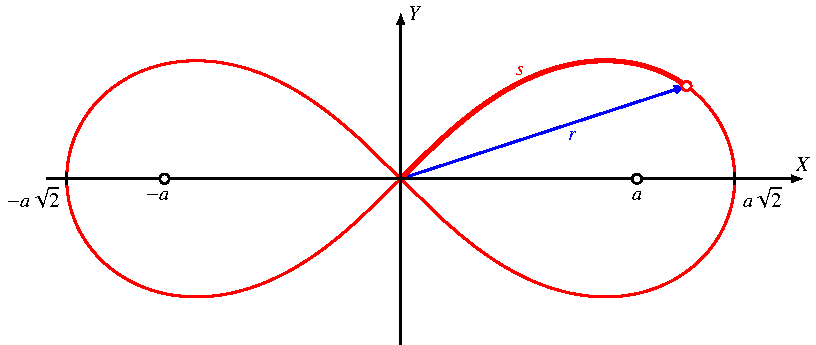
\includegraphics{chapters/110-elliptisch/images/lemniskate.pdf}
\caption{Bogenlänge und Radius der Lemniskate von Bernoulli.
\label{buch:elliptisch:fig:lemniskate}}
\end{figure}
Die Lemniskate von Bernoulli ist die Kurve vierten Grades mit der Gleichung
\begin{equation}
(X^2+Y^2)^2 = 2a^2(X^2-Y^2).
\label{buch:elliptisch:eqn:lemniskate}
\end{equation}
Sie ist in Abbildung~\ref{buch:elliptisch:fig:lemniskate}
dargestellt.
Die beiden Scheitel der Lemniskate befinden sich bei $X_s=\pm a\sqrt{2}$.
Dividiert man die Gleichung der Lemniskate durch $X_s^2=4a^4$ entsteht 
\begin{equation}
\biggl(
\biggl(\frac{X}{a\sqrt{2}}\biggr)^2
+
\biggl(\frac{Y}{a\sqrt{2}}\biggr)^2
\biggr)^2
=
2\frac{a^2}{2a^2}\biggl(
\biggl(\frac{X}{a\sqrt{2}}\biggr)^2
-
\biggl(\frac{Y}{a\sqrt{2}}\biggr)^2
\biggr).
\qquad
\Leftrightarrow
\qquad
(x^2+y^2)^2 = x^2-y^2,
\label{buch:elliptisch:eqn:lemniskatenormiert}
\end{equation}
wobei wir $x=X/a\sqrt{2}$ und $y=Y/a\sqrt{2}$ gesetzt haben.
In dieser Normierung liegen die Scheitel bei $\pm 1$.
Dies ist die Skalierung, die für die Definition des lemniskatischen
Sinus und Kosinus verwendet werden soll.

In Polarkoordinaten $x=r\cos\varphi$ und $y=r\sin\varphi$
gilt nach Einsetzen in \eqref{buch:elliptisch:eqn:lemniskatenormiert}
\begin{equation}
r^4
=
r^2(\cos^2\varphi-\sin^2\varphi)
=
r^2\cos2\varphi
\qquad\Rightarrow\qquad
r^2 = \cos 2\varphi
\label{buch:elliptisch:eqn:lemniskatepolar}
\end{equation}
als Darstellung der Lemniskate in Polardarstellung.
Sie gilt für Winkel $\varphi\in[-\frac{\pi}4,\frac{\pi}4]$ für das
rechte Blatt und $\varphi\in[\frac{3\pi}4,\frac{5\pi}4]$ für das linke
Blatt der Lemniskate.

\subsection{Bogenlänge}
Die Funktionen
\begin{equation}
x(r) = \frac{r}{\sqrt{2}}\sqrt{1+r^2},
\quad
y(r) = \frac{r}{\sqrt{2}}\sqrt{1-r^2}
\label{buch:geometrie:eqn:lemniskateparam}
\end{equation}
erfüllen
\begin{align*}
x(r)^2-y(r)^2
&=
\frac{r^2(1+r^2)}{2}-\frac{r^2(1-r^2)}{2}
\\
&
=
r^4
=
(x(r)^2 + y(r)^2)^2,
\end{align*}
sie stellen also eine Parametrisierung der Lemniskate dar.

Mit Hilfe der Parametrisierung~\eqref{buch:geometrie:eqn:lemniskateparam}
kann man die Länge $s$ des in Abbildung~\ref{buch:elliptisch:fig:lemniskate}
dargestellten Bogens der Lemniskate berechnen.
Dazu benötigt man die Ableitungen nach $r$, die man mit der Produkt- und
Kettenregel berechnen kann:
\begin{align*}
\dot{x}(r)
&=
\frac{\sqrt{1+r^2}}{\sqrt{2}}
+
\frac{r^2}{\sqrt{2}\sqrt{1+r^2}}
&&\Rightarrow&
\dot{x}(r)^2
&=
\frac{1+r^2}{2} +r^2 + \frac{r^4}{2(1+r^2)}
\\
\dot{y}(r)
&=
\frac{\sqrt{1-r^2}}{\sqrt{2}}
-
\frac{r^2}{\sqrt{2}\sqrt{1-r^2}}
&&\Rightarrow&
\dot{y}(r)^2
&=
\frac{1-r^2}{2} -r^2 + \frac{r^4}{2(1-r^2)}
\end{align*}
Die Summe der Quadrate ist
\begin{align*}
\dot{x}(r)^2 + \dot{y}(r)^2
&=
1 + r^4\frac{1-r^2+1+r^2}{2(1+r^2)(1-r^2)}
=
1+r^4\frac{2}{2(1-r^4)}
=
\frac{1-r^4+r^4}{1-r^4}
=
\frac1{1-r^4}.
\end{align*}
Durch Einsetzen in das Integral für die Bogenlänge bekommt man
\begin{equation}
s(r)
=
\int_0^r
\frac{1}{\sqrt{1-t^4}}\,dt.
\label{buch:elliptisch:eqn:lemniskatebogenlaenge}
\end{equation}

%
% Als elliptisches Integral
%
\subsection{Darstellung als elliptisches Integral}
Das unvollständige elliptische Integral erster Art mit Parameter
$k^2=-1$ oder $k=i$ ist
\[
K(r,i)
=
\int_0^x \frac{dt}{\sqrt{(1-t^2)(1-i^2 t^2)}}
=
\int_0^x \frac{dt}{\sqrt{(1-t^2)(1-(-1)t^2)}}
=
\int_0^x \frac{dt}{\sqrt{1-t^4}}
=
s(r).
\]
Der lemniskatische Sinus ist also eine Umkehrfunktion des
elliptischen Integrals erster Art für den speziellen Wert $i$ des
Parameters $k$.

Die Länge des rechten Blattes der Lemniskate wird mit $\varpi$ bezeichnet
und hat den numerischen Wert
\[
\varpi
=
2\int_0^1\sqrt{\frac{1}{1-t^4}}\,dt
=
2.6220575542.
\]
$\varpi$ ist auch als die {\em lemniskatische Konstante} bekannt.
\index{lemniskatische Konstante}%
Der Lemniskatenbogen zwischen dem Nullpunkt und $(1,0)$ hat die Länge
$\varpi/2$.

%
%  Bogenlängenparametrisierung
%
\subsection{Bogenlängenparametrisierung}
Die Lemniskate mit der Gleichung
\[
(X^2+X^2)^2=2(X^2-X^2)
\]
(der Fall $a=1$ in \eqref{buch:elliptisch:eqn:lemniskate})
kann mit Jacobischen elliptischen Funktionen
parametrisiert werden.
Dazu schreibt man
\[
\left.
\begin{aligned}
X(t)
&=
\sqrt{2}\operatorname{cn}(t,k) \operatorname{dn}(t,k)
\\
Y(t)
&=
\phantom{\sqrt{2}}
\operatorname{cn}(t,k) \operatorname{sn}(t,k)
\end{aligned}
\quad\right\}
\qquad\text{mit $k=\displaystyle\frac{1}{\sqrt{2}}$}
\]
und berechnet die beiden Seiten der definierenden Gleichung der
Lemniskate.
Zunächst ist
\begin{align*}
X(t)^2
&=
2\operatorname{cn}(t,k)^2
\operatorname{dn}(t,k)^2
\\
Y(t)^2
&=
\operatorname{cn}(t,k)^2
\operatorname{sn}(t,k)^2
\\
X(t)^2+Y(t)^2
&=
2\operatorname{cn}(t,k)^2
\bigl(
\underbrace{
\operatorname{dn}(t,k)^2
+{\textstyle\frac12}
\operatorname{sn}(t,k)^2
}_{\displaystyle =1}
\bigr)
%\\
%&
=
2\operatorname{cn}(t,k)^2
\\
X(t)^2-Y(t)^2
&=
\operatorname{cn}(t,k)^2
\bigl(
2\operatorname{dn}(t,k)^2 - \operatorname{sn}(t,k)^2
\bigr)
\\
&=
\operatorname{cn}(t,k)^2
\bigl(
2\bigl({\textstyle\frac12}+{\textstyle\frac12}\operatorname{cn}(t,k)^2\bigr)
-
\bigl(1-\operatorname{cn}(t,k)^2\bigr)
\bigr)
\\
&=
2\operatorname{cn}(t,k)^4
\\
\Rightarrow\qquad
(X(t)^2+Y(t)^2)^2
&=
4\operatorname{cn}(t,k)^4
=
2(X(t)^2-Y(t)^2).
\end{align*}
Wir zeigen jetzt, dass dies tatsächlich eine Bogenlängenparametrisierung
der Lemniskate ist.
Dazu berechnen wir die Ableitungen
\begin{align*}
\dot{X}(t)
&=
\sqrt{2}\operatorname{cn}'(t,k)\operatorname{dn}(t,k)
+
\sqrt{2}\operatorname{cn}(t,k)\operatorname{dn}'(t,k)
\\
&=
-\sqrt{2}\operatorname{sn}(t,k)\operatorname{dn}(t,k)^2
-\frac12\sqrt{2}\operatorname{sn}(t,k)\operatorname{cn}(t,k)^2
\\
&=
-\sqrt{2}\operatorname{sn}(t,k)\bigl(
1-{\textstyle\frac12}\operatorname{sn}(t,k)^2
+{\textstyle\frac12}-{\textstyle\frac12}\operatorname{sn}(u,t)^2
\bigr)
\\
&=
\sqrt{2}\operatorname{sn}(t,k)
\bigl(
{\textstyle \frac32}-\operatorname{sn}(t,k)^2
\bigr)
\\
\dot{X}(t)^2
&=
2\operatorname{sn}(t,k)^2
\bigl(
{\textstyle \frac32}-\operatorname{sn}(t,k)^2
\bigr)^2
\\
&=
{\textstyle\frac{9}{2}}\operatorname{sn}(t,k)^2
-
6\operatorname{sn}(t,k)^4
+2\operatorname{sn}(t,k)^6
\\
\dot{Y}(t)
&=
\operatorname{cn}'(t,k)\operatorname{sn}(t,k)
+
\operatorname{cn}(t,k)\operatorname{sn}'(t,k)
\\
&=
-\operatorname{sn}(t,k)^2
\operatorname{dn}(t,k)
+\operatorname{cn}(t,k)^2
\operatorname{dn}(t,k)
\\
&=
\operatorname{dn}(t,k)\bigl(1-2\operatorname{sn}(t,k)^2\bigr)
\\
\dot{Y}(t)^2
&=
\bigl(1-{\textstyle\frac12}\operatorname{sn}(t,k)^2\bigr)
\bigl(1-2\operatorname|{sn}(t,k)^2\bigr)^2
\\
&=
1-{\textstyle\frac{9}{2}}\operatorname{sn}(t,k)^2
+6\operatorname{sn}(t,k)^4
-2\operatorname{sn}(t,k)^6
\\
\dot{X}(t)^2 + \dot{Y}(t)^2
&=
1.
\end{align*}
Dies bedeutet, dass die Bogenlänge zwischen den Parameterwerten $0$ und $s$
\[
\int_0^s
\sqrt{\dot{X}(t)^2 + \dot{Y}(t)^2}
\,dt
=
\int_0^s\,dt
=
s,
\]
der Parameter $t$ ist also ein Bogenlängenparameter.

Die mit dem Faktor $1/\sqrt{2}$ skalierte Standard-Lemniskate mit der
Gleichung
\[
(x^2+y^2)^2 = x^2-y^2
\]
hat daher eine Bogenlängenparametrisierung mit
\begin{equation}
\begin{aligned}
x(t)
&=
\phantom{\frac{1}{\sqrt{2}}}
\operatorname{cn}(\sqrt{2}t,k)\operatorname{dn}(\sqrt{2}t,k)
\\
y(t)
&=
\frac{1}{\sqrt{2}}\operatorname{cn}(\sqrt{2}t,k)\operatorname{sn}(\sqrt{2}t,k)
\end{aligned}
\label{buch:elliptisch:lemniskate:bogenlaenge}
\end{equation}

\subsection{Der lemniskatische Sinus und Kosinus}
Der Sinus Berechnet die Gegenkathete zu einer gegebenen Bogenlänge des
Kreises, er ist die Umkehrfunktion der Funktion, die der Gegenkathete
die Bogenlänge zuordnet.

Daher ist es naheliegend, die Umkehrfunktion von $s(r)$ in 
\eqref{buch:elliptisch:eqn:lemniskatebogenlaenge}
den {\em lemniskatischen Sinus} zu nennen mit der Bezeichnung
$r=\operatorname{sl} s$.

Der Kosinus ist der Sinus des komplementären Winkels.
Auch für die lemniskatische Bogenlänge $s(r)$ lässt sich eine
komplementäre Bogenlänge definieren, nämlich die Bogenlänge zwischen
dem Punkt $(x(r), y(r))$ und $(1,0)$.

Da die Parametrisierung~\eqref{buch:elliptisch:lemniskate:bogenlaenge}
eine Bogenlängenparametrisierung ist, darf man $t=s$ schreiben.
Dann kann man aber auch $r(s)$ daraus berechnen,
es ist
\[
r(s)^2
=
x(s)^2 + y(s)^2
=
\operatorname{cn}(s\sqrt{2},k)^2
\qquad\Rightarrow\qquad
r(s)
=
\operatorname{cn}(s\sqrt{2},k)
\]

\begin{figure}
\centering
\includegraphics{chapters/110-elliptisch/images/slcl.pdf}
\caption{
Lemniskatischer Sinus und Kosinus sowie Sinus und Kosinus
mit derart skaliertem Argument, dass die Funktionen die gleichen Nullstellen
haben.
\label{buch:elliptisch:figure:slcl}}
\end{figure}


%\section*{Übungsaufgaben}
%\rhead{Übungsaufgaben}
%\aufgabetoplevel{chapters/020-exponential/uebungsaufgaben}
%\begin{uebungsaufgaben}
%\uebungsaufgabe{0}
%\uebungsaufgabe{1}
%\end{uebungsaufgaben}



%\begin{appendices}
%\end{appendices}
\vfill
\pagebreak

\ifodd\value{page}\else\null\clearpage\fi
\lhead{Literatur}
\rhead{}
\printbibliography[heading=subbibliography]
\label{buch:literatur}
\end{refsection}


